% ============================================================================
% Cardano Credential Verification: A Complete Study Guide
%
% Comprehensive tutorial covering every concept in the whitepaper
% "Blockchain-Based Professional Credential Verification"
% for readers with no prior blockchain background.
%
% Author: Timothy E. Smith, PE (Virobit)
% Date: February 2026
% ============================================================================

\documentclass[11pt, oneside]{report}

% --- Page Layout -----------------------------------------------------------
\usepackage[
  letterpaper,
  top=1in, bottom=1in, left=1.15in, right=1.15in,
  headheight=14pt
]{geometry}

% --- Core Packages ---------------------------------------------------------
\usepackage[utf8]{inputenc}
\usepackage[T1]{fontenc}
\usepackage{lmodern}
\usepackage{graphicx}
\usepackage{amsmath,amssymb}
\usepackage{booktabs}
\usepackage{tabularx}
\usepackage{longtable}
\usepackage{multirow}
\usepackage{array}
\usepackage{float}
\usepackage{enumitem}
\usepackage{xcolor}
\usepackage{listings}
\usepackage{url}
\usepackage{fancyhdr}
\usepackage{titlesec}
\usepackage{setspace}
\usepackage{parskip}
\usepackage{microtype}

% TikZ for vector graphics
\usepackage{tikz}
\usetikzlibrary{
  shapes.geometric, arrows.meta, positioning, fit, calc,
  backgrounds, decorations.pathreplacing, chains, matrix
}

% Hyperref (loaded last per best practice)
\usepackage[
  bookmarks=true,
  bookmarksnumbered=true,
  colorlinks=true,
  linkcolor=blue!60!black,
  citecolor=blue!60!black,
  urlcolor=blue!60!black,
  pdftitle={Cardano Credential Verification: A Complete Study Guide},
  pdfauthor={Timothy E. Smith, PE},
  pdfsubject={Blockchain, Cardano, Professional Credentials},
]{hyperref}

% --- Colors ----------------------------------------------------------------
\definecolor{codebg}{RGB}{245,245,245}
\definecolor{codeframe}{RGB}{200,200,200}
\definecolor{keyword}{RGB}{0,100,170}
\definecolor{string}{RGB}{170,60,0}
\definecolor{comment}{RGB}{100,130,100}
\definecolor{chaptercolor}{RGB}{30,80,140}
\definecolor{sectioncolor}{RGB}{40,100,160}

% --- Listing Style ---------------------------------------------------------
\lstset{
  basicstyle=\ttfamily\small,
  backgroundcolor=\color{codebg},
  frame=single,
  rulecolor=\color{codeframe},
  keywordstyle=\color{keyword}\bfseries,
  stringstyle=\color{string},
  commentstyle=\color{comment}\itshape,
  breaklines=true,
  breakatwhitespace=true,
  tabsize=2,
  showstringspaces=false,
  captionpos=b,
  aboveskip=8pt,
  belowskip=8pt,
  xleftmargin=4pt,
  xrightmargin=4pt
}

% --- TikZ Styles (shared across all chapters) ------------------------------
\tikzset{
  guidebox/.style={
    draw, rounded corners=4pt, thick, align=center,
    font=\sffamily\small, fill=white, minimum height=1cm
  },
  guideboxwide/.style={
    draw, rounded corners=4pt, thick, align=center,
    font=\sffamily\small, fill=white, minimum height=1cm,
    minimum width=8cm
  },
  guidearrow/.style={
    -{Latex[length=2.5mm]}, thick, color=gray!70!black
  },
  guidelabel/.style={
    font=\sffamily\footnotesize, text=gray!50!black
  },
  tokenbox/.style={
    draw, rounded corners=3pt, thick, align=center,
    minimum height=1.6cm, minimum width=2.8cm,
    font=\sffamily\scriptsize, fill=white
  },
  threatbox/.style={
    draw, rounded corners=3pt, thick, align=center,
    minimum height=1.4cm, minimum width=3.2cm,
    font=\sffamily\scriptsize, fill=white
  },
  phaseblock/.style={
    draw, rounded corners=3pt, thick, align=left,
    text width=3.4cm, minimum height=1.5cm,
    font=\sffamily\scriptsize, fill=white, inner sep=5pt
  },
  seqactor/.style={
    rectangle, draw, fill=gray!15,
    font=\sffamily\small, minimum width=1.8cm, minimum height=0.6cm,
    align=center, text width=1.6cm
  },
  seqarrow/.style={-{Latex[length=2mm]}, thick},
}

% --- Chapter / Section Formatting ------------------------------------------
\titleformat{\chapter}[display]
  {\normalfont\LARGE\bfseries\color{chaptercolor}}
  {\chaptertitlename\ \thechapter}{16pt}{\Huge}
\titleformat{\section}
  {\normalfont\Large\bfseries\color{sectioncolor}}
  {\thesection}{1em}{}
\titleformat{\subsection}
  {\normalfont\large\bfseries}
  {\thesubsection}{1em}{}

% --- Header / Footer -------------------------------------------------------
\pagestyle{fancy}
\fancyhf{}
\fancyhead[L]{\small\leftmark}
\fancyhead[R]{\small Cardano Credential Study Guide}
\fancyfoot[C]{\thepage}
\renewcommand{\headrulewidth}{0.4pt}

% --- Custom Commands -------------------------------------------------------
\newcolumntype{L}[1]{>{\raggedright\arraybackslash}p{#1}}
\newcolumntype{C}[1]{>{\centering\arraybackslash}p{#1}}

\newcommand{\keyterm}[1]{\textbf{\textcolor{chaptercolor}{#1}}}
\newcommand{\cip}[1]{\texttt{CIP-#1}}
\newcommand{\ada}{\textsc{ada}}

% ============================================================================
\begin{document}

% --- Title Page ------------------------------------------------------------
\begin{titlepage}
\centering
\vspace*{2cm}

{\Huge\bfseries\color{chaptercolor}
Cardano Credential Verification\\[0.4cm]
\Large A Complete Study Guide}

\vspace{1.5cm}

{\large\itshape
Comprehensive Tutorial for the Whitepaper\\
``Blockchain-Based Professional Credential Verification:\\
A Cardano Smart Contract Architecture for License Management\\
and Digital Signatures'' (v3.1)}

\vspace{2cm}

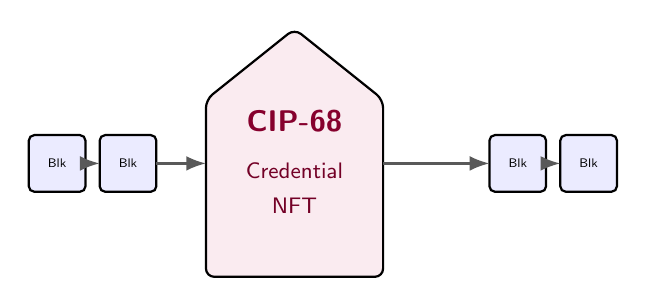
\begin{tikzpicture}[scale=0.9, every node/.style={transform shape}]
  % Shield shape for credential
  \draw[thick, fill=purple!8, rounded corners=3pt]
    (0,0) -- (2.5,0) -- (2.5,2.5) -- (1.25,3.5) -- (0,2.5) -- cycle;
  \node[font=\sffamily\large\bfseries, text=purple!70!black] at (1.25,2.2) {CIP-68};
  \node[font=\sffamily\small, text=purple!60!black] at (1.25,1.5) {Credential};
  \node[font=\sffamily\small, text=purple!60!black] at (1.25,1.0) {NFT};

  % Chain links
  \foreach \x in {-2.5, -1.5, 4.0, 5.0} {
    \draw[thick, fill=blue!8, rounded corners=2pt]
      (\x, 1.2) rectangle (\x+0.8, 2.0);
  }
  \draw[thick, guidearrow] (-1.5+0.8, 1.6) -- (0, 1.6);
  \draw[thick, guidearrow] (2.5, 1.6) -- (4.0, 1.6);
  \draw[thick, guidearrow] (-2.5+0.8, 1.6) -- (-1.5, 1.6);
  \draw[thick, guidearrow] (4.0+0.8, 1.6) -- (5.0, 1.6);

  \node[font=\sffamily\tiny] at (-2.1, 1.6) {Blk};
  \node[font=\sffamily\tiny] at (-1.1, 1.6) {Blk};
  \node[font=\sffamily\tiny] at (4.4, 1.6) {Blk};
  \node[font=\sffamily\tiny] at (5.4, 1.6) {Blk};
\end{tikzpicture}

\vspace{2cm}

{\Large Timothy E. Smith, PE}\\[0.3cm]
{\large Virobit Research}\\[0.3cm]
{\large February 2026}

\vfill

{\small
Open Source --- MIT License\\
\url{https://github.com/virobit/license_management_using_cardano}
}

\end{titlepage}

% --- Table of Contents -----------------------------------------------------
\tableofcontents
\newpage

% --- Preface ---------------------------------------------------------------
\chapter*{Preface}
\addcontentsline{toc}{chapter}{Preface}

This study guide is a companion to the research paper \textit{``Blockchain-Based Professional Credential Verification: A Cardano Smart Contract Architecture for License Management and Digital Signatures''} (v3.1, February 2026). While the paper presents the architecture for an academic audience, this guide is written for \textbf{anyone who wants to understand how the system works}, regardless of technical background.

\textbf{No prior knowledge of blockchain, cryptography, or Cardano is assumed.} Every concept referenced in the whitepaper is explained from first principles, with diagrams, analogies, and code examples. By the end of this guide, you will understand:

\begin{itemize}[nosep]
  \item How blockchains work and why they are useful for credential verification
  \item How Cardano's unique architecture (eUTxO, native tokens, Plutus) differs from other blockchains
  \item What every Cardano Improvement Proposal (CIP) referenced in the paper does
  \item How smart contracts enforce credential rules on Cardano
  \item How the complete credential lifecycle works --- from issuance through revocation
  \item How multi-party document signing is implemented
  \item How privacy and legal compliance (GDPR, ESIGN, eIDAS) are achieved
  \item How the \texttt{cardano-license} software package works
  \item What the v4.0 roadmap delivers
\end{itemize}

Each chapter builds on the previous one, so we recommend reading in order. Key terms are \keyterm{highlighted in blue} when first introduced, and a comprehensive glossary is provided at the end.

\vspace{1cm}
\noindent\textit{This guide was prepared with assistance from Claude Code (Anthropic). All technical claims, architectural decisions, and editorial judgments are the sole responsibility of the author.}

\newpage

% ============================================================================
% CHAPTER 1: Blockchain Fundamentals
% ============================================================================
% ===========================================================================
% Chapter 1 — Blockchain Fundamentals
% Study Guide: Blockchain & Cardano Credential Verification
% ===========================================================================

% ---- Shared TikZ style definitions for this guide -------------------------
\tikzset{
  guidebox/.style={draw, rounded corners=4pt, thick, align=center,
                   font=\sffamily\small, fill=white, minimum height=1cm},
  guidearrow/.style={-{Latex[length=2.5mm]}, thick, color=gray!70!black},
  guidelabel/.style={font=\sffamily\footnotesize, text=gray!50!black},
}

% Convenience colours (semantic names for repeated fills)
\colorlet{inputcolor}{blue!8}
\colorlet{processcolor}{green!8}
\colorlet{outputcolor}{orange!8}
\colorlet{blockchaincolor}{purple!8}
\colorlet{securitycolor}{red!6}
\colorlet{intermediatecolor}{yellow!8}
\colorlet{neutralcolor}{gray!10}

% ===================================================================
\chapter{Blockchain Fundamentals}
\label{ch:blockchain-fundamentals}
% ===================================================================

This chapter introduces the foundational concepts you need before we touch a
single line of Cardano code.  Every idea is explained from scratch---no prior
knowledge of blockchain, cryptography, or distributed systems is assumed.  By
the end of this chapter you will understand \emph{what} a blockchain is,
\emph{why} it works, and \emph{how} Cardano improves on earlier designs.
These building blocks are essential for the credential-verification system we
will construct in later chapters.

% -------------------------------------------------------------------
\section{What Is a Blockchain?}
\label{sec:what-is-blockchain}
% -------------------------------------------------------------------

Imagine a notebook that sits in the centre of a town square.  Every time
someone makes a deal---say, Alice sells a bicycle to Bob---they walk to the
square and write the transaction in the notebook for everyone to see.  Once a
page is full, a town clerk stamps it with a unique seal, tears it out, and
staples it to the previous page.  The seal on each new page includes a
reference to the seal on the page before it.  If anyone tried to rip out a
page in the middle and replace it, the seals would no longer match and the
entire town would immediately notice.

A \textbf{blockchain} is the digital version of that notebook.  Instead of
pages we have \emph{blocks}; instead of a staple we have a
\emph{cryptographic hash} (explained in Section~\ref{sec:hashing}); and
instead of one notebook in a square, thousands of identical copies are
maintained by computers all over the world.

\subsection{Blocks}

A \textbf{block} is a bundle of data.  In a financial blockchain the data is
a list of transactions (``Alice sent 10 tokens to Bob''), but blocks can hold
any kind of information---credential issuances, votes, supply-chain events,
or software licence grants.  Every block also carries a small header that
contains bookkeeping metadata: a timestamp, a reference to the previous
block, and the result of running all the block's data through a hash function
(Section~\ref{sec:hashing}).

Each block can be thought of as a sealed envelope.  Once the envelope is
sealed (the block is added to the chain), its contents cannot be changed
without breaking the seal.  Because every subsequent envelope references the
seal of the one before it, altering a single envelope would require
re-sealing every envelope that comes after---a task that is computationally
infeasible on a well-established chain.

\subsection{Chains and Immutability}

The word \emph{chain} refers to the way blocks are linked.  Block~2 contains
the hash of Block~1; Block~3 contains the hash of Block~2; and so on.  This
creates an unbroken lineage all the way back to Block~0 (the \emph{genesis
block}).  If someone modifies even a single byte inside Block~1, its hash
changes, which means Block~2's ``previous hash'' field no longer matches,
which invalidates Block~3, and so on.  The entire chain after the tampered
block collapses like a row of dominoes.

This property is called \textbf{immutability}: once data is recorded in a
block and enough subsequent blocks have been added on top, it is
extraordinarily difficult to alter.  Immutability is one of the key reasons
blockchains are attractive for credential verification---a licence recorded
on-chain cannot be silently edited or back-dated.

\begin{figure}[htbp]
\centering
\begin{tikzpicture}[node distance=0.6cm]

  % --- Block 0 (Genesis) ---
  \node[guidebox, fill=blockchaincolor, minimum width=3.8cm, minimum height=3.2cm]
    (b0) {};
  \node[font=\sffamily\bfseries\small, anchor=north] at ([yshift=-3pt]b0.north)
    {Block 0 (Genesis)};
  \node[guidebox, fill=neutralcolor, minimum width=3.2cm, font=\ttfamily\scriptsize]
    (b0hash) at ([yshift=-0.55cm]b0.north) {Prev: 0000...0000};
  \node[guidebox, fill=inputcolor, minimum width=3.2cm, text width=2.8cm,
        font=\sffamily\scriptsize, align=center]
    (b0data) at ([yshift=-0.45cm]b0hash.south)
    {Data:\\``Network starts''};
  \node[guidebox, fill=intermediatecolor, minimum width=3.2cm,
        font=\ttfamily\scriptsize]
    (b0own) at ([yshift=-0.35cm]b0data.south) {Hash: 7a3f...e1b2};

  % --- Block 1 ---
  \node[guidebox, fill=blockchaincolor, minimum width=3.8cm, minimum height=3.2cm,
        right=1.4cm of b0]
    (b1) {};
  \node[font=\sffamily\bfseries\small, anchor=north] at ([yshift=-3pt]b1.north)
    {Block 1};
  \node[guidebox, fill=neutralcolor, minimum width=3.2cm, font=\ttfamily\scriptsize]
    (b1hash) at ([yshift=-0.55cm]b1.north) {Prev: 7a3f...e1b2};
  \node[guidebox, fill=inputcolor, minimum width=3.2cm, text width=2.8cm,
        font=\sffamily\scriptsize, align=center]
    (b1data) at ([yshift=-0.45cm]b1hash.south)
    {Data:\\``Alice $\to$ Bob: 10 T''};
  \node[guidebox, fill=intermediatecolor, minimum width=3.2cm,
        font=\ttfamily\scriptsize]
    (b1own) at ([yshift=-0.35cm]b1data.south) {Hash: c9d1...4f8a};

  % --- Block 2 ---
  \node[guidebox, fill=blockchaincolor, minimum width=3.8cm, minimum height=3.2cm,
        right=1.4cm of b1]
    (b2) {};
  \node[font=\sffamily\bfseries\small, anchor=north] at ([yshift=-3pt]b2.north)
    {Block 2};
  \node[guidebox, fill=neutralcolor, minimum width=3.2cm, font=\ttfamily\scriptsize]
    (b2hash) at ([yshift=-0.55cm]b2.north) {Prev: c9d1...4f8a};
  \node[guidebox, fill=inputcolor, minimum width=3.2cm, text width=2.8cm,
        font=\sffamily\scriptsize, align=center]
    (b2data) at ([yshift=-0.45cm]b2hash.south)
    {Data:\\``Bob $\to$ Carol: 5 T''};
  \node[guidebox, fill=intermediatecolor, minimum width=3.2cm,
        font=\ttfamily\scriptsize]
    (b2own) at ([yshift=-0.35cm]b2data.south) {Hash: 21ef...b7c3};

  % --- Block 3 ---
  \node[guidebox, fill=blockchaincolor, minimum width=3.8cm, minimum height=3.2cm,
        right=1.4cm of b2]
    (b3) {};
  \node[font=\sffamily\bfseries\small, anchor=north] at ([yshift=-3pt]b3.north)
    {Block 3};
  \node[guidebox, fill=neutralcolor, minimum width=3.2cm, font=\ttfamily\scriptsize]
    (b3hash) at ([yshift=-0.55cm]b3.north) {Prev: 21ef...b7c3};
  \node[guidebox, fill=inputcolor, minimum width=3.2cm, text width=2.8cm,
        font=\sffamily\scriptsize, align=center]
    (b3data) at ([yshift=-0.45cm]b3hash.south)
    {Data:\\``Carol $\to$ Dave: 3 T''};
  \node[guidebox, fill=intermediatecolor, minimum width=3.2cm,
        font=\ttfamily\scriptsize]
    (b3own) at ([yshift=-0.35cm]b3data.south) {Hash: 58ab...d9e4};

  % --- Chain arrows ---
  \draw[guidearrow, line width=1.2pt] (b0own.east) -- ++(0.25,0)
    |- ([yshift=0.0cm]b1hash.west);
  \draw[guidearrow, line width=1.2pt] (b1own.east) -- ++(0.25,0)
    |- ([yshift=0.0cm]b2hash.west);
  \draw[guidearrow, line width=1.2pt] (b2own.east) -- ++(0.25,0)
    |- ([yshift=0.0cm]b3hash.west);

  % --- Annotation ---
  \node[guidelabel, text width=4cm, align=center]
    at ([yshift=-0.9cm]$(b1.south)!0.5!(b2.south)$)
    {Each block's hash feeds into the next block,\\forming an unbreakable chain.};

\end{tikzpicture}
\caption{A blockchain of four blocks.  Each block stores data plus the hash
of the preceding block. Changing Block~1 would invalidate every
subsequent hash.}
\label{fig:blockchain-chain}
\end{figure}


% -------------------------------------------------------------------
\section{Consensus Mechanisms}
\label{sec:consensus}
% -------------------------------------------------------------------

If thousands of computers around the world each hold a copy of the
blockchain, who decides which new block gets added next?  What stops a
malicious actor from broadcasting a fake block that credits themselves with a
million tokens?  These questions are answered by a \textbf{consensus
mechanism}---a set of rules that all participants (called \emph{nodes}) follow
to agree on the next valid block.

Without consensus, a distributed ledger would quickly descend into chaos.
Different nodes would have different versions of reality, and there would be
no way to tell which one is ``true.''  Consensus mechanisms solve this by
making it expensive or statistically improbable for any single party to
dominate the block-production process.

\subsection{Proof of Work (PoW)}

Bitcoin, the first blockchain, uses \textbf{Proof of Work}.  In PoW, nodes
(called \emph{miners}) compete to solve a mathematical puzzle.  The puzzle is
simple to describe but computationally exhausting: find a number (called a
\emph{nonce}) such that when you hash the block header together with that
nonce, the resulting hash starts with a certain number of leading zeros.
There is no shortcut; miners must try billions of nonce values per second
until one of them stumbles on a valid answer.

The miner who finds the answer first broadcasts the new block to the network,
and the other miners verify (verification is fast---just one hash
computation) and accept it.  The winning miner is rewarded with
newly created cryptocurrency.  The difficulty of the puzzle is automatically
adjusted so that, on average, one new block is found every ten minutes
(in Bitcoin's case).

PoW is remarkably secure---attacking it would require controlling more than
half of the entire network's computing power, which for Bitcoin would cost
billions of dollars in hardware and electricity.  The downside is precisely
that electricity cost: Bitcoin's annual energy consumption rivals that of
some small countries.  This is the primary motivation for alternative
consensus mechanisms.

\subsection{Proof of Stake (PoS) and Cardano's Ouroboros}

Cardano uses \textbf{Proof of Stake}, specifically a protocol called
\textbf{Ouroboros}.  Instead of burning electricity to solve puzzles, PoS
selects the next block producer based on how much cryptocurrency they have
\emph{staked} (locked up as collateral).  Think of it as a raffle: if you
hold 2\% of all staked tokens, you have roughly a 2\% chance of being chosen
to produce the next block.  There is no puzzle to solve, so the energy cost
is negligible---a standard laptop can run a Cardano stake pool.

Ouroboros divides time into \emph{epochs} (each lasting five days) and
further into \emph{slots} (each one second long).  At the beginning of each
epoch a lottery determines which stake-pool operator is eligible to produce
a block in each slot.  If the designated leader is online, they produce the
block and earn rewards; if not, the slot is skipped and the next eligible
leader takes over.  In practice, a new block appears roughly every 20
seconds.

The security guarantee of Ouroboros has been formally proven in
peer-reviewed academic papers---a distinguishing feature of Cardano.  As
long as at least 51\% of the staked ada is controlled by honest participants,
the protocol guarantees that the chain will grow correctly and that
double-spending is impossible.

\begin{figure}[htbp]
\centering
\begin{tikzpicture}[node distance=0.5cm]

  % ---- PoW side ----
  \node[font=\sffamily\bfseries\large, color=red!60!black] (powtitle)
    {Proof of Work};

  \node[guidebox, fill=securitycolor, minimum width=4.5cm, below=0.5cm of powtitle,
        text width=4cm]
    (powmine) {Miners compete\\to solve puzzle};
  \node[guidebox, fill=intermediatecolor, minimum width=4.5cm, below=0.5cm of powmine,
        text width=4cm]
    (powhw) {Requires specialized\\hardware (ASICs)};
  \node[guidebox, fill=outputcolor, minimum width=4.5cm, below=0.5cm of powhw,
        text width=4cm]
    (powenergy) {High energy\\consumption};
  \node[guidebox, fill=neutralcolor, minimum width=4.5cm, below=0.5cm of powenergy,
        text width=4cm]
    (powsec) {Security from\\computational cost};
  \node[guidebox, fill=inputcolor, minimum width=4.5cm, below=0.5cm of powsec,
        text width=4cm]
    (powex) {Example: Bitcoin\\$\sim$10 min blocks};

  \draw[guidearrow] (powmine) -- (powhw);
  \draw[guidearrow] (powhw) -- (powenergy);
  \draw[guidearrow] (powenergy) -- (powsec);
  \draw[guidearrow] (powsec) -- (powex);

  % ---- PoS side ----
  \node[font=\sffamily\bfseries\large, color=green!50!black,
        right=3.5cm of powtitle]
    (postitle) {Proof of Stake};

  \node[guidebox, fill=processcolor, minimum width=4.5cm, below=0.5cm of postitle,
        text width=4cm]
    (posstake) {Validators stake\\tokens as collateral};
  \node[guidebox, fill=intermediatecolor, minimum width=4.5cm, below=0.5cm of posstake,
        text width=4cm]
    (poshw) {Runs on standard\\consumer hardware};
  \node[guidebox, fill=processcolor, minimum width=4.5cm, below=0.5cm of poshw,
        text width=4cm]
    (posenergy) {Minimal energy\\consumption};
  \node[guidebox, fill=neutralcolor, minimum width=4.5cm, below=0.5cm of posenergy,
        text width=4cm]
    (possec) {Security from\\economic stake};
  \node[guidebox, fill=inputcolor, minimum width=4.5cm, below=0.5cm of possec,
        text width=4cm]
    (posex) {Example: Cardano\\$\sim$20 sec blocks};

  \draw[guidearrow] (posstake) -- (poshw);
  \draw[guidearrow] (poshw) -- (posenergy);
  \draw[guidearrow] (posenergy) -- (possec);
  \draw[guidearrow] (possec) -- (posex);

  % ---- VS divider ----
  \node[font=\sffamily\Huge\bfseries, color=gray!40,
        anchor=center]
    at ($(powmine.east)!0.5!(posstake.west) + (0,-1.7)$) {vs};

\end{tikzpicture}
\caption{Proof of Work versus Proof of Stake.  PoS eliminates the enormous
energy expenditure of PoW by replacing computational puzzles with
economic incentives.}
\label{fig:pow-vs-pos}
\end{figure}


% -------------------------------------------------------------------
\section{Public Key Cryptography}
\label{sec:public-key-crypto}
% -------------------------------------------------------------------

Before we can understand how transactions are authorised on a blockchain, we
need to grasp \textbf{public key cryptography} (also called \emph{asymmetric
cryptography}).  This is the mathematical machinery that lets you prove you
own something without revealing a secret.

\subsection{The Mailbox Analogy}

Imagine you install a mailbox on your front lawn.  The mailbox has a slot
(the \textbf{public key}) through which anyone can drop a letter, but it also
has a lock (the \textbf{private key}) that only you can open.  You freely
share your address (the slot location) with the world, but you never share
the lock's key.  Anyone can send you mail; only you can read it.

In blockchain terms, your \emph{public key} (or a shortened version called
your \emph{address}) is what you share so that others can send you
cryptocurrency or verify your signatures.  Your \emph{private key} is the
secret that lets you spend your funds or sign documents.  If someone obtains
your private key, they can impersonate you---guard it as carefully as you
would guard the key to a safety-deposit box.

\subsection{Digital Signatures}

A \textbf{digital signature} is the blockchain equivalent of a handwritten
signature on a cheque, but far more secure.  When you want to send a
transaction, your wallet software takes the transaction data and combines it
with your private key using a mathematical algorithm (Cardano uses
\emph{Ed25519}).  The output is a short string of bytes---the signature.

Anyone who has your public key can then run a verification algorithm on the
(transaction, signature) pair.  If the signature is valid, they know two
things with mathematical certainty:

\begin{enumerate}
  \item \textbf{Authenticity}: The transaction was created by whoever holds
        the corresponding private key.
  \item \textbf{Integrity}: The transaction has not been modified since it
        was signed---not even by a single bit.
\end{enumerate}

This is what makes blockchain transactions trustworthy.  There is no bank or
notary in the middle; the mathematics itself provides the proof.  For our
credential-verification system, this same mechanism will let a licensing
authority sign a credential, and any third party can verify that signature
without contacting the authority.

\subsection{Keys, Addresses, and Wallets}

In practice, a \emph{wallet} is a piece of software that manages one or more
private keys on your behalf.  When you ``create a wallet,'' the software
generates a random private key, derives the corresponding public key, and
further derives an \emph{address} (a shorter, human-readable encoding of the
public key, often with a checksum to catch typos).  On Cardano, addresses
start with \texttt{addr1...} on mainnet and \texttt{addr\_test1...} on the
test network.

A single wallet can contain many key pairs, all derived from a single master
seed phrase (typically 24 words).  This hierarchical key derivation means you
only need to back up those 24 words to recover all of your keys and
addresses.

\begin{figure}[htbp]
\centering
\begin{tikzpicture}[node distance=0.7cm]

  % ---- Signer side ----
  \node[font=\sffamily\bfseries] (signertitle) {Signer (Alice)};

  \node[guidebox, fill=securitycolor, minimum width=3.4cm, text width=3cm, below=0.4cm of signertitle]
    (privkey) {Private Key\\{\ttfamily\scriptsize sk\_a3f8...}};

  \node[guidebox, fill=inputcolor, minimum width=3.4cm, text width=3cm, below=0.5cm of privkey]
    (txdata) {Transaction Data\\{\scriptsize ``Send 50 ada to Bob''}};

  \node[guidebox, fill=processcolor, minimum width=3.4cm, minimum height=1.2cm,
        text width=3cm, below=0.5cm of txdata]
    (signfn) {\textbf{Sign}\\{\scriptsize Ed25519 algorithm}};

  \node[guidebox, fill=outputcolor, minimum width=3.4cm, text width=3cm, below=0.5cm of signfn]
    (sig) {Signature\\{\ttfamily\scriptsize 9c2b...7e41}};

  \draw[guidearrow] (privkey) -- (signfn);
  \draw[guidearrow] (txdata) -- (signfn);
  \draw[guidearrow] (signfn) -- (sig);

  % ---- Transmission ----
  \node[guidelabel, text width=2cm, align=center, right=2.2cm of signfn] (transmit) {Broadcast to\\network};
  \draw[guidearrow, dashed] (sig.east) -- ++(1.0,0) |- (transmit.west);

  % ---- Verifier side ----
  \node[font=\sffamily\bfseries, right=6.5cm of signertitle]
    (vertitle) {Verifier (Any Node)};

  \node[guidebox, fill=inputcolor, minimum width=3.4cm, text width=3cm, below=0.4cm of vertitle]
    (pubkey) {Public Key\\{\ttfamily\scriptsize vk\_7d1e...}};

  \node[guidebox, fill=inputcolor, minimum width=3.4cm, text width=3cm, below=0.5cm of pubkey]
    (rxdata) {Transaction Data\\{\scriptsize (received)};};

  \node[guidebox, fill=inputcolor, minimum width=3.4cm, text width=3cm, below=0.5cm of rxdata]
    (rxsig) {Signature\\{\ttfamily\scriptsize 9c2b...7e41}};

  \node[guidebox, fill=processcolor, minimum width=3.4cm, minimum height=1.2cm,
        text width=3cm, below=0.5cm of rxsig]
    (verifyfn) {\textbf{Verify}\\{\scriptsize Ed25519 algorithm}};

  \draw[guidearrow] (pubkey.south) -- ++(0,-0.15) -| ([xshift=-0.6cm]verifyfn.north);
  \draw[guidearrow] (rxdata) -- (rxsig);
  \draw[guidearrow] (rxsig) -- (verifyfn);

  % ---- Result ----
  \node[guidebox, fill=processcolor, minimum width=3.4cm, below=0.5cm of verifyfn,
        font=\sffamily\bfseries\small, text=green!50!black]
    (valid) {Valid --- Accept};

  \node[guidebox, fill=securitycolor, minimum width=3.4cm, right=0.5cm of valid,
        font=\sffamily\bfseries\small, text=red!60!black]
    (invalid) {Invalid --- Reject};

  \draw[guidearrow, color=green!50!black] (verifyfn) -- (valid);
  \draw[guidearrow, color=red!50!black, dashed] (verifyfn.east) -- ++(0.5,0)
    |- (invalid.west);

  % ---- Labels ----
  \node[guidelabel] at ([yshift=-0.6cm]$(valid.south)!0.5!(invalid.south)$)
    {Only the holder of the private key can produce a valid signature.};

\end{tikzpicture}
\caption{Digital signature flow.  Alice signs with her private key; any node
verifies with her public key.  If the data or signature is altered, verification fails.}
\label{fig:sign-verify}
\end{figure}


% -------------------------------------------------------------------
\section{Hashing}
\label{sec:hashing}
% -------------------------------------------------------------------

Hashing is one of the most important primitives in all of blockchain
technology.  A \textbf{hash function} takes an input of any size---a single
character, a novel, an entire database---and produces an output (called a
\emph{digest} or simply a \emph{hash}) of a fixed size.  SHA-256, for
example, always produces a 256-bit (32-byte) output regardless of whether the
input is one byte or one terabyte.

\subsection{One-Way Functions}

The critical property of a cryptographic hash function is that it is
\textbf{one-way}: given the output, there is no feasible way to reconstruct
the input.  This is analogous to a meat grinder: you can push a steak in and
get ground beef out, but you cannot reassemble the steak from the ground
beef.  Even a tiny change to the input---flipping a single bit---produces a
completely different hash, a property known as the \emph{avalanche effect}.

This one-way property is what makes the blockchain's hash-chain tamper-proof.
An attacker cannot start with a desired hash and work backwards to craft a
block that matches.  They would have to try inputs at random, which for a
256-bit hash means searching through $2^{256}$ possibilities---a number
larger than the estimated count of atoms in the observable universe.

\subsection{SHA-256 and Blake2b}

\textbf{SHA-256} (Secure Hash Algorithm, 256 bits) is the hash function used
by Bitcoin.  It was designed by the U.S.\ National Security Agency and has
been extensively studied for over two decades.  It produces a 256-bit hash
(commonly displayed as a 64-character hexadecimal string).

\textbf{Blake2b} is a newer hash function that is faster than SHA-256 on
modern hardware while maintaining equivalent security.  Cardano uses
Blake2b-256 (256-bit output) for most on-chain hashing, including the
computation of transaction IDs and policy IDs.  It also uses Blake2b-224
(224-bit output, i.e.\ 28 bytes) for deriving the key-hash portion of
addresses.

For our purposes the choice between SHA-256 and Blake2b is an implementation
detail---both behave like ideal one-way functions.  What matters is
understanding the \emph{concept}: any input produces a fixed-size fingerprint,
and that fingerprint cannot be reversed.

\subsection{Practical Examples}

To build intuition, here are some example hashes (SHA-256, shown as
hexadecimal):

\begin{center}
\small
\begin{tabular}{lp{10cm}}
\toprule
\textbf{Input} & \textbf{SHA-256 Hash (first 16 hex chars\ldots)} \\
\midrule
\texttt{"hello"} & \texttt{2cf24dba5fb0a30e...} \\
\texttt{"Hello"} & \texttt{185f8db32271fe25...} \\
\texttt{"hello!"} & \texttt{ce06092fb948d936...} \\
\texttt{"hello" (repeated 1000$\times$)} & \texttt{f1d3ff8443297732...} \\
\bottomrule
\end{tabular}
\end{center}

Notice that capitalising the ``h'' or adding an exclamation mark produces a
completely unrelated hash.  There is no pattern, no partial similarity---this
is the avalanche effect in action.  Also note that the hash length is the
same regardless of whether the input is 5 characters or 5\,000.

\begin{figure}[htbp]
\centering
\begin{tikzpicture}[node distance=0.6cm]

  % ---- Inputs ----
  \node[guidebox, fill=inputcolor, minimum width=3.5cm] (in1)
    {{\scriptsize\texttt{"hello"}} \quad (5 bytes)};
  \node[guidebox, fill=inputcolor, minimum width=3.5cm, below=0.4cm of in1] (in2)
    {{\scriptsize\texttt{"Blockchain!"}} \quad (11 bytes)};
  \node[guidebox, fill=inputcolor, minimum width=3.5cm, below=0.4cm of in2] (in3)
    {{\scriptsize 4.2\,GB video file}};

  \node[font=\sffamily\bfseries\small, above=0.3cm of in1] {Any-size Input};

  % ---- Hash function ----
  \node[guidebox, fill=processcolor, minimum width=3.5cm, minimum height=2.8cm,
        text width=3cm, right=2.0cm of in2, font=\sffamily\bfseries]
    (hashfn) {Hash\\Function\\[3pt]{\footnotesize SHA-256 / Blake2b-256}};

  % ---- Output ----
  \node[guidebox, fill=outputcolor, minimum width=4.2cm, right=2.0cm of hashfn]
    (out1) {{\scriptsize\texttt{2cf24dba...}} (32 bytes)};
  \node[guidebox, fill=outputcolor, minimum width=4.2cm, below=0.4cm of out1]
    (out2) {{\scriptsize\texttt{a1075db5...}} (32 bytes)};
  \node[guidebox, fill=outputcolor, minimum width=4.2cm, below=0.4cm of out2]
    (out3) {{\scriptsize\texttt{7f83b165...}} (32 bytes)};

  \node[font=\sffamily\bfseries\small, above=0.3cm of out1] {Fixed-size Output};

  % ---- Arrows ----
  \draw[guidearrow] (in1.east) -- ++(0.4,0) |- ([yshift=0.6cm]hashfn.west);
  \draw[guidearrow] (in2.east) -- (hashfn.west);
  \draw[guidearrow] (in3.east) -- ++(0.4,0) |- ([yshift=-0.6cm]hashfn.west);

  \draw[guidearrow] ([yshift=0.6cm]hashfn.east) -- ++(0.4,0) |- (out1.west);
  \draw[guidearrow] (hashfn.east) -- (out2.west);
  \draw[guidearrow] ([yshift=-0.6cm]hashfn.east) -- ++(0.4,0) |- (out3.west);

  % ---- One-way label ----
  \draw[{Latex[length=2.5mm]}-, thick, color=red!60!black, dashed]
    ([yshift=-0.3cm]hashfn.east) -- ++(0.7,0)
    node[midway, below=3pt, font=\sffamily\tiny\bfseries, color=red!60!black]
    {ONE-WAY};

  % ---- Bottom annotation ----
  \node[guidelabel, text width=12cm, align=center]
    at ([yshift=-1.0cm]$(in3.south)!0.5!(out3.south)$)
    {Regardless of input size, the output is always exactly 32 bytes.
     The function is one-way: you cannot recover the input from the hash.};

\end{tikzpicture}
\caption{A hash function maps any-size input to a fixed-size output.
The process is deterministic (same input always yields the same hash)
but irreversible.}
\label{fig:hash-function}
\end{figure}


% -------------------------------------------------------------------
\section{Transaction Models: Account vs UTxO}
\label{sec:utxo-vs-account}
% -------------------------------------------------------------------

How does a blockchain keep track of who owns what?  There are two dominant
models, and understanding the difference is \emph{critical} for working with
Cardano.

\subsection{The Account Model (Ethereum)}

The \textbf{account model} works exactly like a bank account.  Each address
has a single balance, and a transaction simply debits one account and credits
another.  If Alice has 100 tokens and sends 30 to Bob, the ledger updates
two numbers: Alice's balance becomes 70 and Bob's balance becomes 30 (or
increases by 30 if he already had some).

This is intuitive and easy to reason about, which is why Ethereum chose it.
However, it introduces complications around ordering (what if two
transactions try to spend from Alice's account simultaneously?) and requires
global state tracking---every node must maintain and agree on the current
balance of every account.

\subsection{The UTxO Model (Bitcoin and Cardano)}

Cardano and Bitcoin use the \textbf{Unspent Transaction Output (UTxO)}
model.  This is best understood by analogy to physical cash.

Imagine Alice has a \$50 bill and a \$20 bill in her wallet (two UTxOs).  She
wants to pay Bob \$60.  She cannot tear the bills in half; she must hand over
both bills (\$70 total) and receive \$10 in change.  After the transaction,
Alice has one new UTxO worth \$10 and Bob has one new UTxO worth \$60.  The
original \$50 and \$20 UTxOs are now ``spent'' and can never be used again.

More precisely, every transaction \emph{consumes} one or more existing UTxOs
(the \textbf{inputs}) and \emph{produces} one or more new UTxOs (the
\textbf{outputs}).  The sum of the inputs must equal the sum of the outputs
plus any transaction fee.  A UTxO can only be spent once---this is how
double-spending is prevented.

The UTxO model has several advantages for our credential system:

\begin{itemize}
  \item \textbf{Determinism}: A transaction's validity depends only on its
        inputs, not on any global state.  You can validate a transaction
        offline.
  \item \textbf{Parallelism}: Transactions that consume different UTxOs are
        independent and can be processed in parallel.
  \item \textbf{Auditability}: You can trace the complete history of every
        token by following the UTxO chain backwards, which is ideal for
        credential provenance.
\end{itemize}

\subsection{Cardano's Extended UTxO (EUTxO)}

Cardano extends the basic UTxO model with two powerful additions:

\begin{enumerate}
  \item \textbf{Datum}: Each UTxO can carry an arbitrary piece of data (the
        \emph{datum}).  This is where we will store credential metadata---the
        licence holder's name, expiry date, credential type, and so on.
  \item \textbf{Validator scripts}: Instead of being locked by a simple
        public-key hash, a UTxO can be locked by a \emph{Plutus script} (a
        program that runs on-chain).  The script decides whether a
        transaction is allowed to consume the UTxO, based on the datum, the
        \emph{redeemer} (an argument supplied by the spender), and the full
        \emph{script context} (information about the transaction).
\end{enumerate}

This ``Extended UTxO'' (EUTxO) model is what makes Cardano a programmable
blockchain while retaining the determinism and parallelism benefits of the
original UTxO design.  We will explore Plutus scripts in detail in a later
chapter.

\begin{figure}[htbp]
\centering
\begin{tikzpicture}[node distance=0.5cm]

  % ============================================================
  %  Transaction box
  % ============================================================
  \node[guidebox, fill=processcolor, minimum width=3.0cm, minimum height=2.2cm,
        text width=2.6cm, font=\sffamily\bfseries]
    (tx) {Transaction\\[2pt]{\footnotesize Fee: 0.2 ada}};

  \node[font=\sffamily\bfseries\small, color=blue!60!black]
    at ([yshift=1.6cm]tx.north) {Cardano UTxO Transaction};

  % ============================================================
  %  Inputs (left side)
  % ============================================================
  \node[font=\sffamily\bfseries\footnotesize, color=blue!60!black,
        left=3.8cm of tx, yshift=0.9cm]
    (inlabel) {Inputs (UTxOs consumed)};

  \node[guidebox, fill=inputcolor, minimum width=3.4cm, text width=3.0cm,
        below=0.25cm of inlabel, align=center]
    (utxo1) {UTxO \#1\\{\scriptsize Alice: 50 ada}\\
             {\scriptsize\color{gray}TxId: a3f8...\#0}};

  \node[guidebox, fill=inputcolor, minimum width=3.4cm, text width=3.0cm,
        below=0.35cm of utxo1, align=center]
    (utxo2) {UTxO \#2\\{\scriptsize Alice: 20 ada}\\
             {\scriptsize\color{gray}TxId: b7c1...\#2}};

  \node[guidelabel, below=0.2cm of utxo2]
    {Total in: 70 ada};

  % ============================================================
  %  Outputs (right side)
  % ============================================================
  \node[font=\sffamily\bfseries\footnotesize, color=orange!70!black,
        right=3.8cm of tx, yshift=0.9cm]
    (outlabel) {Outputs (new UTxOs created)};

  \node[guidebox, fill=outputcolor, minimum width=3.4cm, text width=3.0cm,
        below=0.25cm of outlabel, align=center]
    (out1) {UTxO \#A\\{\scriptsize Bob: 60 ada}\\
            {\scriptsize\color{gray}TxId: d4e9...\#0}};

  \node[guidebox, fill=outputcolor, minimum width=3.4cm, text width=3.0cm,
        below=0.35cm of out1, align=center]
    (out2) {UTxO \#B (change)\\{\scriptsize Alice: 9.8 ada}\\
            {\scriptsize\color{gray}TxId: d4e9...\#1}};

  \node[guidelabel, below=0.2cm of out2]
    {Total out: 69.8 ada (+0.2 fee)};

  % ============================================================
  %  Arrows
  % ============================================================
  \draw[guidearrow, line width=1.2pt] (utxo1.east) -- (tx.west |- utxo1.east);
  \draw[guidearrow, line width=1.2pt] (utxo2.east) -- (tx.west |- utxo2.east);
  \draw[guidearrow, line width=1.2pt] (tx.east |- out1.west) -- (out1.west);
  \draw[guidearrow, line width=1.2pt] (tx.east |- out2.west) -- (out2.west);

  % ============================================================
  %  Spent markers
  % ============================================================
  \node[font=\sffamily\bfseries\scriptsize, color=red!70!black,
        rotate=20] at ([xshift=-0.3cm, yshift=0.25cm]utxo1.north east) {SPENT};
  \node[font=\sffamily\bfseries\scriptsize, color=red!70!black,
        rotate=20] at ([xshift=-0.3cm, yshift=0.25cm]utxo2.north east) {SPENT};

  % ============================================================
  %  Annotation
  % ============================================================
  \node[guidelabel, text width=13cm, align=center]
    at ([yshift=-1.2cm]tx.south)
    {Alice consumes two UTxOs (50 + 20 = 70 ada), sends 60 to Bob, and
     receives 9.8 ada as change.  The 0.2 ada transaction fee goes to the
     stake pool that produced the block.  The consumed UTxOs are permanently
     marked as spent.};

\end{tikzpicture}
\caption{Anatomy of a UTxO transaction.  Inputs are consumed (destroyed)
and outputs are created.  The sum of inputs equals the sum of outputs
plus the fee.}
\label{fig:utxo-transaction}
\end{figure}


% -------------------------------------------------------------------
\section{What Is Cardano?}
\label{sec:what-is-cardano}
% -------------------------------------------------------------------

\textbf{Cardano} is a third-generation, open-source, proof-of-stake
blockchain platform.  It was founded in 2015 by Charles Hoskinson (a
co-founder of Ethereum) and is developed primarily by Input Output Global
(IOG), with support from the Cardano Foundation and Emurgo.

\subsection{Generational Context}

Blockchains are sometimes categorised by ``generation'':

\begin{description}
  \item[First generation (Bitcoin, 2009):] Introduced decentralised digital
    money and the basic blockchain data structure.  Limited to simple
    value-transfer transactions.
  \item[Second generation (Ethereum, 2015):] Added smart contracts---programs
    that run on the blockchain---enabling decentralised applications (dApps),
    token standards, and DeFi.  However, Ethereum faces scalability
    challenges and uses an account-based model that can lead to
    non-deterministic transaction outcomes.
  \item[Third generation (Cardano, 2017):] Aims to solve the remaining
    challenges of scalability, interoperability, and sustainability through
    peer-reviewed research, formal methods, and a layered architecture.
\end{description}

Cardano is distinctive in its \emph{research-first} approach.  Every major
design decision---the Ouroboros consensus protocol, the EUTxO ledger model,
the Plutus smart-contract platform---was first published as a peer-reviewed
academic paper and subjected to formal verification before being implemented.
This makes Cardano one of the most rigorously designed blockchain platforms
in existence.

\subsection{Architecture and Timing}

Cardano's architecture is divided into two layers:

\begin{itemize}
  \item \textbf{Cardano Settlement Layer (CSL)}: Handles the transfer of ada
        (Cardano's native cryptocurrency) and native tokens.  This is the
        accounting layer.
  \item \textbf{Cardano Computation Layer (CCL)}: Handles smart contracts
        (Plutus and Aiken scripts).  Separating computation from settlement
        allows each layer to be optimised independently.
\end{itemize}

Key timing parameters:

\begin{itemize}
  \item \textbf{Slot duration}: 1 second.
  \item \textbf{Block production}: A block is produced approximately every
        \textbf{20 seconds} on average (not every slot has a block; the slot
        leader lottery means roughly 1 in 20 slots produce a block).
  \item \textbf{Epoch length}: 432\,000 slots = \textbf{5 days}.
  \item \textbf{Transaction finality}: After approximately \textbf{5--10
        minutes} (about 15--30 blocks), a transaction is considered
        practically irreversible.  For high-value applications, waiting for
        one full epoch provides overwhelming assurance.
\end{itemize}

\subsection{Native Multi-Asset Support}

One of Cardano's most powerful features---and one we rely on heavily for
credential verification---is \textbf{native multi-asset support}.  On
Ethereum, creating a new type of token requires deploying a smart contract
(e.g., an ERC-20 contract).  On Cardano, custom tokens are \emph{native}:
they live directly on the ledger, are transferred using the same mechanisms
as ada, and incur no additional smart-contract execution cost for simple
transfers.

Every native token is identified by a \textbf{policy ID} (the hash of the
minting policy script that controls its creation) and a \textbf{token name}
(an arbitrary byte string up to 32 bytes).  The minting policy script defines
the rules under which tokens can be minted (created) or burned (destroyed).
For credential tokens, we will write policies that allow only the authorised
licensing body to mint, and that make the tokens non-fungible (each one is
unique to a specific licence holder).

\subsection{Formal Verification Heritage}

Cardano's smart-contract language, Plutus, is based on Haskell---a purely
functional programming language with a strong type system.  This choice was
deliberate: pure functions and strong types make it dramatically easier to
formally verify that a program does what it claims.  Additionally, the newer
\textbf{Aiken} language provides a more developer-friendly syntax while
compiling to the same underlying Plutus Core, offering the same on-chain
guarantees with a gentler learning curve.

For a credential system, formal verification is not an academic luxury---it
is a practical necessity.  A bug in a minting policy could allow counterfeit
licences; a bug in a validator could lock legitimate credentials forever.
Cardano's tooling helps us avoid these catastrophic outcomes.

\begin{figure}[htbp]
\centering
\begin{tikzpicture}[node distance=0.5cm]

  % ---- Timeline ----
  \draw[thick, gray!50] (0,0) -- (15,0);

  % Epoch bracket
  \draw[thick, blockchaincolor, decorate, decoration={brace, amplitude=8pt, raise=2pt}]
    (0.5,0.3) -- (14.5,0.3)
    node[midway, above=12pt, font=\sffamily\bfseries\small, color=purple!70!black]
    {1 Epoch = 432{,}000 slots = 5 days};

  % Slot ticks
  \foreach \x in {1,2,3,4,5,6,7,8,9,10,11,12,13,14} {
    \draw[gray!40] (\x,-0.15) -- (\x,0.15);
  }

  % Blocks (some slots produce blocks, some don't)
  \foreach \x/\lbl in {1/1, 4/2, 5/3, 8/4, 11/5, 14/6} {
    \node[guidebox, fill=blockchaincolor, minimum width=0.7cm,
          minimum height=0.7cm, font=\sffamily\bfseries\scriptsize]
      at (\x, -0.9) {\lbl};
    \draw[guidearrow, thin] (\x,-0.15) -- (\x,-0.5);
  }

  % Empty slot labels
  \foreach \x in {2,3,6,7,9,10,12,13} {
    \node[font=\scriptsize, color=gray!50] at (\x,-0.55) {--};
  }

  % Labels
  \node[guidelabel] at (0,-0.9) {Slot:};
  \node[guidelabel, font=\sffamily\scriptsize] at (1,-1.7) {1s};
  \node[guidelabel, font=\sffamily\scriptsize] at (4,-1.7) {4s};
  \node[guidelabel, font=\sffamily\scriptsize] at (14,-1.7) {14s};

  % Annotation below
  \node[guidelabel, text width=14cm, align=center] at (7.5, -2.6)
    {Each slot is 1 second.  Only $\sim$1 in 20 slots produces a block
     ($\sim$20\,s average block time).  Empty slots are normal.
     Finality is reached after $\sim$15--30 confirmations
     ($\sim$5--10 minutes).};

  % Block time label
  \draw[thick, orange!70!black, decorate,
        decoration={brace, amplitude=6pt, mirror, raise=2pt}]
    (1,-1.1) -- (4,-1.1)
    node[midway, below=10pt, font=\sffamily\scriptsize, color=orange!70!black]
    {$\sim$20s between blocks};

\end{tikzpicture}
\caption{Cardano timing: slots, blocks, and epochs.  Not every slot produces
a block; the average inter-block time is approximately 20 seconds.}
\label{fig:cardano-timing}
\end{figure}

\bigskip

\begin{center}
\begin{tikzpicture}
  \node[guidebox, fill=blockchaincolor, minimum width=14cm, minimum height=2.5cm,
        text width=13cm, align=left, font=\sffamily\small] {
    \textbf{Chapter Summary}\\[6pt]
    \begin{tabular}{@{}ll@{}}
    \textbf{Blockchain} & Append-only ledger of hash-linked blocks; immutable once confirmed.\\
    \textbf{Consensus}  & Ouroboros PoS: validators stake ada; no mining hardware needed.\\
    \textbf{Cryptography} & Public/private key pairs enable digital signatures and ownership.\\
    \textbf{Hashing}    & One-way function producing fixed-size fingerprints (Blake2b on Cardano).\\
    \textbf{UTxO model} & Transactions consume UTxOs and create new ones (like spending cash).\\
    \textbf{Cardano}    & Third-gen, peer-reviewed, EUTxO, native tokens, $\sim$20s blocks, $\sim$5 min finality.\\
    \end{tabular}
  };
\end{tikzpicture}
\end{center}


% ============================================================================
% CHAPTER 2: Cardano Architecture
% ============================================================================
% ============================================================================
% Chapter 2: Cardano's Extended UTxO Model and Architecture
% Study Guide for Blockchain Credential Verification
%
% This file contains ONLY chapter content. It must be included from a
% main document that provides the preamble, TikZ libraries, and
% \begin{document} wrapper.
%
% Required TikZ libraries (load in preamble):
%   shapes.geometric, arrows.meta, positioning, fit, calc, backgrounds,
%   decorations.pathreplacing, patterns, chains
%
% Required packages: amsmath, amssymb, xcolor, listings, enumitem, booktabs
% ============================================================================

% --- Chapter-local TikZ styles ---------------------------------------------
\tikzset{
  guidebox/.style={
    draw, rounded corners=4pt, thick, align=center,
    font=\sffamily\small, fill=white, minimum height=1cm
  },
  guidearrow/.style={
    -{Latex[length=2.5mm]}, thick, color=gray!70!black
  },
  guidelabel/.style={
    font=\sffamily\footnotesize, text=gray!50!black
  },
}

% ============================================================================
\chapter{Cardano's Extended UTxO Model and Architecture}
\label{ch:cardano-architecture}
% ============================================================================

In Chapter~1 we established the foundational concepts of blockchain
technology: cryptographic hashing, public-key cryptography, consensus
mechanisms, and the distinction between the account model (Ethereum) and
the UTxO model (Bitcoin). We saw that Bitcoin's Unspent Transaction
Output model treats value like physical coins---each output is a
discrete, indivisible unit that must be consumed entirely when spent,
with any excess returned as ``change.'' This chapter takes that
foundation and builds upon it, exploring how Cardano extends the UTxO
model into something far more powerful: a programmable, data-rich ledger
capable of supporting complex credential verification workflows.

Understanding Cardano's architecture is not merely academic. Every
design decision in the credential verification system described in later
chapters---from how license tokens are minted, to how revocation
propagates, to how transaction costs are predicted---flows directly from
the architectural properties covered here. By the end of this chapter
you will understand \emph{why} Cardano was chosen for this system, not
just \emph{that} it was chosen.


% ============================================================================
\section{The Extended UTxO (eUTxO) Model}
\label{sec:eutxo}
% ============================================================================

\subsection{From Bitcoin's UTxO to Cardano's eUTxO}

Recall from Chapter~1 that Bitcoin's UTxO model works like a collection
of sealed envelopes, each containing a specific amount of currency and a
lock that only the recipient's private key can open. When Alice sends Bob
3~BTC, she does not modify a balance in an account database. Instead, she
\emph{consumes} one or more existing UTxOs she controls and
\emph{produces} new UTxOs: one paying Bob 3~BTC, and possibly another
returning change to herself. The consumed UTxOs cease to exist; the new
UTxOs become available for future spending. This is fundamentally
different from the account model, where a transfer simply decrements
one balance and increments another.

Bitcoin's UTxOs, however, are limited. Each UTxO carries only two pieces
of information: a value (how much BTC it holds) and a locking script
(who can spend it, typically requiring a specific public key signature).
There is no way to attach arbitrary data to a UTxO, no way for a
spending transaction to provide arguments to the locking script, and the
locking script itself has only minimal awareness of the transaction that
attempts to spend it.

Cardano's Extended UTxO model preserves the core advantages of the UTxO
approach---determinism, parallelism, and simple local validation---while
adding three critical extensions that transform UTxOs from simple value
carriers into programmable data containers. These three extensions are
\textbf{Datums}, \textbf{Redeemers}, and \textbf{Script Context}.

\subsection{Datums: Data Attached to UTxOs}

A \textbf{Datum} is an arbitrary piece of structured data that can be
attached to any UTxO. Think of it as a label glued to the outside of the
sealed envelope. In Bitcoin, the envelope only tells you how much money
is inside and whose key opens it. In Cardano, the envelope can also
carry a data payload---a license number, an expiration date, a list of
authorized signers, a document hash, or any other structured information
that a validator script might need to examine.

Datums are encoded using Cardano's Plutus data format (CBOR-serialized
algebraic data types), and they can range from simple integers to deeply
nested records with multiple fields. For credential verification, datums
are the mechanism that turns a native token from a bare proof of
existence into a rich credential record. A license NFT's reference token,
for example, carries an inline datum containing the license type,
jurisdiction, issue date, licensee identity, and a mutable status
field---all readable by any party querying the blockchain.

Before the Vasil hard fork (September 2022), datums had to be provided
separately from the UTxO and matched by hash, which required the
spending party to know the datum's content in advance. The introduction
of \textbf{inline datums} (CIP-32) changed this: the datum is stored
directly within the UTxO on the ledger, making it readable by anyone
without requiring off-chain coordination. This is what makes instant
credential verification possible---a verifier simply reads the inline
datum from the reference token UTxO.

\subsection{Redeemers: Data Provided When Spending}

A \textbf{Redeemer} is a piece of data provided by the party attempting
to spend a script-locked UTxO. If the datum is the label on the
envelope, the redeemer is the message you hand to the guard who decides
whether to let you open it. The redeemer does not exist on the
blockchain until the moment a spending transaction is submitted---it is
transaction-specific, ephemeral data that the validator script receives
as an argument.

Redeemers enable a single validator script to support multiple
operations. For example, the Signature Collection Validator in our
credential system accepts three different redeemer values: ``Collect''
(a signer deposits tokens), ``Finalize'' (the authority completes the
process), and ``Reclaim'' (a signer cancels and retrieves tokens). The
script examines the redeemer to determine which set of validation rules
to apply, then checks the transaction against those rules. This is
analogous to a single contract with multiple clauses---the redeemer
selects which clause is being invoked.

The redeemer pattern is powerful because it separates the \emph{what}
(the action being performed) from the \emph{how} (the validation logic).
A single script address can manage complex multi-step workflows without
requiring separate contracts for each step.

\subsection{Script Context: The Transaction in Full}

The \textbf{Script Context} is the complete set of information about the
transaction that is made available to the validator script during
execution. This includes all inputs being consumed, all outputs being
produced, all minting and burning operations, all signatures present,
the valid time range (slot interval), and the transaction fee. The script
context is what gives Cardano validators their power: they can inspect
the \emph{entire} transaction, not just the single UTxO being spent.

This is a crucial distinction from Bitcoin's Script, which can only see
the specific input being validated. A Cardano validator can enforce rules
like ``this UTxO may only be spent if the transaction also produces an
output paying at least 50 ADA to address X'' or ``this UTxO may only be
consumed if the transaction mints exactly one token under policy Y.''
For credential systems, script context enables validators to verify that
a signer's deposit transaction includes the correct tokens, references
the correct document hash, and falls within the validity window---all in
a single atomic check.

\subsection{Determinism: The Key Advantage}

The combination of datums, redeemers, and script context produces a
property that is perhaps the eUTxO model's most important advantage over
account-based models: \textbf{deterministic execution}. Given the same
inputs, datum, redeemer, and script context, a Cardano validator always
produces the same result, regardless of what other transactions are
happening on the network at the same time.

In Ethereum's account model, the outcome of a smart contract call
depends on the global state at the moment of execution, which can change
between the time a transaction is submitted and when it is included in a
block. This leads to failed transactions that still consume gas,
front-running attacks where miners reorder transactions for profit, and
unpredictable costs. In Cardano's eUTxO model, you can validate a
transaction completely off-chain before submitting it. If it validates
locally, it \emph{will} validate on-chain. The fee is known exactly. The
outcome is guaranteed. For a credential verification system handling
professional licenses and legal signatures, this predictability is not
merely convenient---it is essential.

\begin{figure}[htbp]
\centering
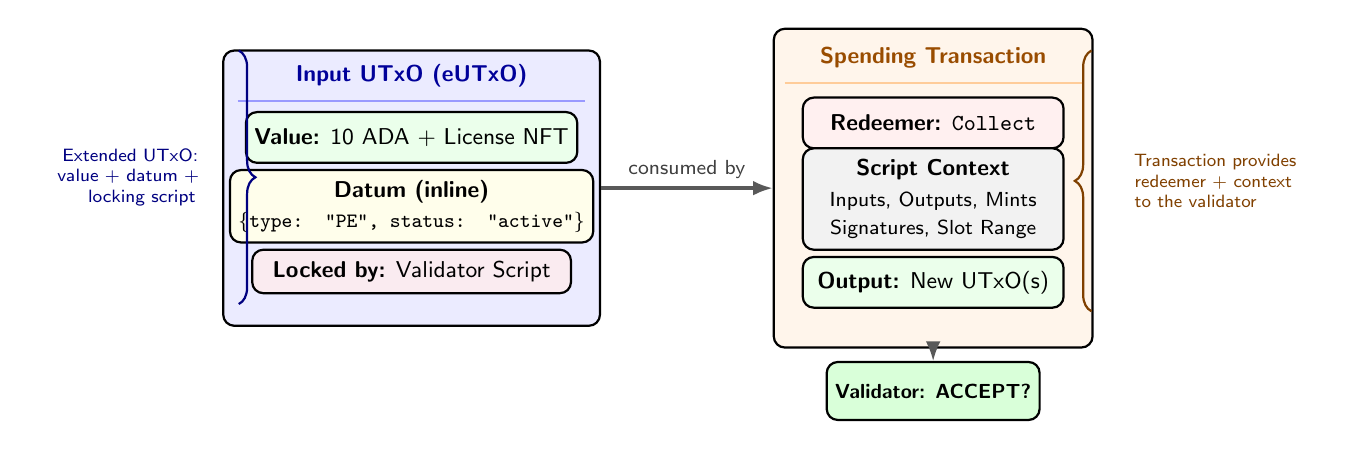
\begin{tikzpicture}[
  scale=0.92,
  every node/.style={transform shape},
]
  % ── Consumed UTxO (input) ──────────────────────────────────────
  \node[guidebox, fill=blue!8, minimum width=5.2cm, minimum height=3.8cm]
    (input) at (-4.2, 0) {};
  \node[font=\sffamily\small\bfseries, text=blue!60!black]
    at (-4.2, 1.55) {Input UTxO (eUTxO)};
  \draw[thick, blue!40] (-6.6, 1.2) -- (-1.8, 1.2);

  % Value area
  \node[guidebox, fill=green!8, minimum width=4.4cm, minimum height=0.7cm]
    at (-4.2, 0.7) {\textbf{Value:} 10 ADA + License NFT};

  % Datum area
  \node[guidebox, fill=yellow!8, minimum width=4.4cm, minimum height=1.0cm]
    at (-4.2, -0.25) {%
      \textbf{Datum (inline)}\\[1pt]
      \footnotesize\texttt{\{type: "PE", status: "active"\}}};

  % Locking script label
  \node[guidebox, fill=purple!8, minimum width=4.4cm, minimum height=0.6cm]
    at (-4.2, -1.15) {\textbf{Locked by:} Validator Script};

  % ── Spending Transaction ───────────────────────────────────────
  \node[guidebox, fill=orange!8, minimum width=4.4cm, minimum height=4.4cm]
    (tx) at (3.0, 0) {};
  \node[font=\sffamily\small\bfseries, text=orange!60!black]
    at (3.0, 1.8) {Spending Transaction};
  \draw[thick, orange!40] (0.95, 1.45) -- (5.05, 1.45);

  % Redeemer
  \node[guidebox, fill=red!6, minimum width=3.6cm, minimum height=0.7cm]
    at (3.0, 0.9) {\textbf{Redeemer:} \texttt{Collect}};

  % Script Context
  \node[guidebox, fill=gray!10, minimum width=3.6cm, minimum height=1.4cm]
    at (3.0, -0.15) {%
      \textbf{Script Context}\\[1pt]
      \footnotesize Inputs, Outputs, Mints\\
      \footnotesize Signatures, Slot Range};

  % Output
  \node[guidebox, fill=green!8, minimum width=3.6cm, minimum height=0.7cm]
    at (3.0, -1.3) {\textbf{Output:} New UTxO(s)};

  % ── Arrows ─────────────────────────────────────────────────────
  \draw[guidearrow, line width=1.2pt]
    (input.east) -- node[above, guidelabel] {consumed by} (tx.west);

  % ── Validator decision ─────────────────────────────────────────
  \node[guidebox, fill=green!15, minimum width=2.8cm, minimum height=0.8cm,
        font=\sffamily\footnotesize\bfseries]
    (accept) at (3.0, -2.8) {Validator: ACCEPT?};

  \draw[guidearrow, dashed] (tx.south) -- (accept.north);

  % Annotations
  \draw[decorate, decoration={brace, amplitude=6pt, raise=3pt},
        thick, blue!50!black]
    (-6.7, 1.9) -- (-6.7, -1.6)
    node[midway, left=10pt, font=\sffamily\scriptsize, text=blue!50!black,
         align=right, text width=2.2cm]
    {Extended UTxO:\\value + datum +\\locking script};

  \draw[decorate, decoration={brace, amplitude=6pt, mirror, raise=3pt},
        thick, orange!50!black]
    (5.3, 1.9) -- (5.3, -1.7)
    node[midway, right=10pt, font=\sffamily\scriptsize, text=orange!50!black,
         align=left, text width=2.4cm]
    {Transaction provides\\redeemer + context\\to the validator};
\end{tikzpicture}
\caption{Anatomy of an Extended UTxO and a spending transaction. The input
UTxO carries a value, an inline datum, and is locked by a validator script.
The spending transaction provides a redeemer (the action to perform) and
the script context (complete transaction data). The validator examines all
three---datum, redeemer, context---to decide whether to accept or reject
the spend.}
\label{fig:eutxo-anatomy}
\end{figure}


% ============================================================================
\section{Native Multi-Asset Framework}
\label{sec:native-assets}
% ============================================================================

\subsection{Tokens Without Smart Contracts}

One of Cardano's most distinctive architectural features---and a primary
reason it was chosen for the credential verification system---is its
\textbf{native multi-asset framework}. On Ethereum, creating a custom
token requires deploying a smart contract (ERC-20 for fungible tokens,
ERC-721 for non-fungible tokens). Every transfer of that token requires
executing the smart contract, consuming gas, and relying on the contract
code being correct. A bug in an ERC-20 contract can freeze or drain
every token it manages, as numerous exploits have demonstrated.

On Cardano, custom tokens---both fungible and non-fungible---exist at
the \emph{ledger level}, the same level as ADA itself. They are tracked
by the same UTxO accounting rules, validated by the same consensus
mechanism, and transferred with the same transaction logic. No smart
contract execution is required to transfer a native token from one
address to another. The token simply moves from one UTxO to another,
just like ADA. This means that native tokens inherit all of the security
guarantees of the base currency: they cannot be double-spent, they
cannot be created out of thin air (except by an authorized minting
policy), and they cannot be frozen by a buggy contract.

For a credential verification system, this architecture is
transformative. A professional license NFT on Cardano is not a record in
a smart contract's internal storage---it is a first-class asset on the
ledger, as ``real'' as ADA itself. Transferring it costs only a standard
transaction fee (\textasciitilde0.17~ADA), not a smart contract
execution fee. Verifying its existence requires only a UTxO query, not a
contract call.

\subsection{Policy ID and Asset Name}

Every native token on Cardano is identified by a two-part identifier:

\begin{description}[leftmargin=1.5cm, labelwidth=1.3cm]
  \item[Policy ID] A 28-byte (56 hex character) Blake2b-224 hash of the
    \textbf{minting policy script}. The minting policy is the script
    that defines who can create (mint) or destroy (burn) tokens under
    this policy. Because the Policy ID is a cryptographic hash of the
    script, it is deterministic and unforgeable---anyone can independently
    verify which script produced a given Policy ID. If the California
    Board of Professional Engineers publishes their Policy ID, any
    verifier can confirm that a license token was minted under that exact
    policy.

  \item[Asset Name] A human-readable (or arbitrary byte string) name
    within a policy, up to 32 bytes. For credential tokens, this
    typically encodes the credential type or identifier, such as
    \texttt{LIC\_PE\_2026\_00042} or \texttt{SIG\_TOKEN}. The
    combination of Policy ID and Asset Name uniquely identifies every
    token on the Cardano ledger.
\end{description}

This two-part identification scheme is analogous to a domain name
system: the Policy ID is like the domain (controlled by the authority),
and the Asset Name is like a path within that domain (chosen by the
authority for each token type). A forger cannot create a token with the
California Board's Policy ID because they do not possess the authority
key that the minting policy requires.

\subsection{Multi-Asset Bundles in UTxOs}

A single Cardano UTxO can carry \emph{multiple} tokens alongside ADA.
This is called a \textbf{multi-asset bundle} (or simply a ``value
bundle''). Unlike Bitcoin, where each UTxO carries only the native
currency, a Cardano UTxO's value field is a nested map:

\begin{quote}
\texttt{Value = Map<PolicyId, Map<AssetName, Quantity>>}
\end{quote}

A single UTxO might contain 5~ADA, plus 100 signature tokens under
Policy~A, plus 1 license NFT under Policy~B, plus 1 validity token
under Policy~C. This bundling capability is essential for the credential
system's signature workflow, where a signer must deposit multiple token
types in a single atomic transaction.

\begin{figure}[htbp]
\centering
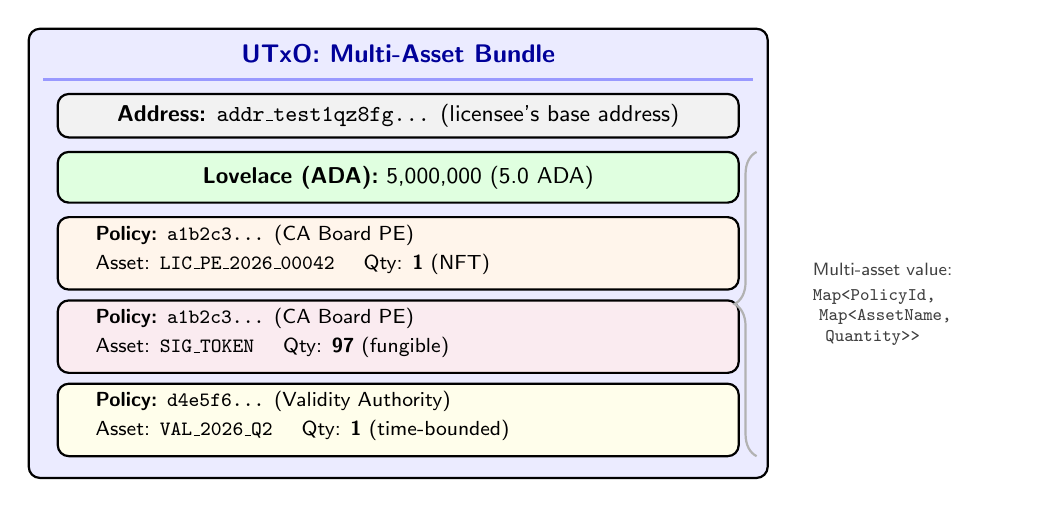
\begin{tikzpicture}[
  scale=0.92,
  every node/.style={transform shape},
]
  % ── Main UTxO container ────────────────────────────────────────
  \node[guidebox, fill=blue!8, minimum width=10.2cm, minimum height=6.2cm]
    (utxo) at (0, 0) {};
  \node[font=\sffamily\bfseries, text=blue!60!black]
    at (0, 2.75) {UTxO: Multi-Asset Bundle};
  \draw[thick, blue!40] (-4.9, 2.4) -- (4.9, 2.4);

  % ── Address ────────────────────────────────────────────────────
  \node[guidebox, fill=gray!10, minimum width=9.4cm, minimum height=0.6cm]
    at (0, 1.9)
    {\textbf{Address:}
     \texttt{addr\_test1qz8fg...} (licensee's base address)};

  % ── ADA value ──────────────────────────────────────────────────
  \node[guidebox, fill=green!12, minimum width=9.4cm, minimum height=0.7cm]
    (ada) at (0, 1.05)
    {\textbf{Lovelace (ADA):} 5{,}000{,}000 (5.0 ADA)};

  % ── Token rows ─────────────────────────────────────────────────
  % Token 1: License NFT
  \node[guidebox, fill=orange!8, minimum width=9.4cm, minimum height=1.0cm]
    (tok1) at (0, 0.0) {};
  \node[font=\sffamily\footnotesize, anchor=west] at (-4.3, 0.25)
    {\textbf{Policy:} \texttt{a1b2c3...} (CA Board PE)};
  \node[font=\sffamily\footnotesize, anchor=west] at (-4.3, -0.15)
    {Asset: \texttt{LIC\_PE\_2026\_00042} \quad Qty: \textbf{1} (NFT)};

  % Token 2: Signature tokens
  \node[guidebox, fill=purple!8, minimum width=9.4cm, minimum height=1.0cm]
    (tok2) at (0, -1.15) {};
  \node[font=\sffamily\footnotesize, anchor=west] at (-4.3, -0.9)
    {\textbf{Policy:} \texttt{a1b2c3...} (CA Board PE)};
  \node[font=\sffamily\footnotesize, anchor=west] at (-4.3, -1.3)
    {Asset: \texttt{SIG\_TOKEN} \quad Qty: \textbf{97} (fungible)};

  % Token 3: Validity token
  \node[guidebox, fill=yellow!8, minimum width=9.4cm, minimum height=1.0cm]
    (tok3) at (0, -2.3) {};
  \node[font=\sffamily\footnotesize, anchor=west] at (-4.3, -2.05)
    {\textbf{Policy:} \texttt{d4e5f6...} (Validity Authority)};
  \node[font=\sffamily\footnotesize, anchor=west] at (-4.3, -2.45)
    {Asset: \texttt{VAL\_2026\_Q2} \quad Qty: \textbf{1} (time-bounded)};

  % ── Braces for value map ───────────────────────────────────────
  \draw[decorate, decoration={brace, amplitude=8pt, mirror, raise=4pt},
        thick, gray!60]
    (5.1, 1.4) -- (5.1, -2.8)
    node[midway, right=14pt, font=\sffamily\scriptsize, text=gray!50!black,
         align=left, text width=2.6cm]
    {Multi-asset value:\\[2pt]
     \texttt{Map<PolicyId,}\\
     \texttt{\ Map<AssetName,}\\
     \texttt{\ \ Quantity>{}>}};
\end{tikzpicture}
\caption{A single Cardano UTxO carrying a multi-asset bundle: ADA (required
for the minimum UTxO deposit), a license NFT, 97 fungible signature tokens,
and a time-bounded validity token. All reside in a single UTxO under the
licensee's address. The tokens span two different Policy IDs, demonstrating
that a UTxO can hold tokens from multiple authorities.}
\label{fig:multi-asset-utxo}
\end{figure}


% ============================================================================
\section{Minimum UTxO (minUTxO) Deposit}
\label{sec:min-utxo}
% ============================================================================

\subsection{The Problem: Ledger Bloat}

Every UTxO on the Cardano blockchain consumes storage space on every
full node in the network. Unlike account-based systems where an empty
account can be cheaply represented (or garbage-collected), every UTxO
persists until explicitly consumed by a transaction. If creating UTxOs
were free, an attacker could create billions of tiny, worthless UTxOs to
bloat the ledger, degrading performance for all participants. This is
known as the \textbf{dust attack} problem.

Cardano addresses this with the \textbf{minimum UTxO deposit}
requirement: every UTxO must contain a minimum amount of ADA,
proportional to the size of the UTxO (including any native tokens and
datums it carries). The formula is based on a protocol parameter called
\texttt{coinsPerUTxOByte} (currently 4,310 lovelace per byte). In
practice, this works out to approximately:

\begin{itemize}[nosep]
  \item \textbf{\textasciitilde1.0 ADA} for a simple ADA-only UTxO
  \item \textbf{\textasciitilde1.5 ADA} for a UTxO carrying a single
    native token
  \item \textbf{\textasciitilde2.0 ADA} for a UTxO carrying multiple
    tokens or a datum
  \item \textbf{\textasciitilde2.5--5.0 ADA} for a UTxO with a large
    inline datum (e.g., CIP-68 reference tokens)
\end{itemize}

\subsection{The Apartment Deposit Analogy}

The minUTxO deposit works exactly like a security deposit on an
apartment. When you move in (create a UTxO carrying native tokens), the
landlord (the Cardano protocol) requires you to put down a deposit (the
minimum ADA). This deposit is not a fee---it is not spent or consumed.
It sits in the UTxO, locked alongside your tokens. When you move out
(consume the UTxO by spending its contents), you get the deposit back.
The ADA returns to you as part of the transaction's change output.

This has a direct impact on the economics of the credential system.
Every license NFT, every batch of signature tokens, and every validity
token requires an accompanying ADA deposit of approximately 1.5--2.0
ADA. For a board issuing 10,000 licenses, this means roughly 20,000~ADA
(\textasciitilde\$6,000 at \$0.30/ADA) must be available as working
capital for deposits, even though the ADA is fully recoverable when
tokens are burned or consolidated.

\subsection{Why This Matters for Credential Systems}

Understanding the minUTxO deposit is crucial for three reasons:

\begin{enumerate}[nosep]
  \item \textbf{Cost Planning.} While the deposit is recoverable, it
    represents locked capital. A licensing board must budget for both
    transaction fees (consumed, non-recoverable) and minUTxO deposits
    (locked, recoverable).
  \item \textbf{Token Consolidation.} If a licensee accumulates many
    small UTxOs (e.g., receiving signature tokens in separate batches),
    the total locked ADA can grow substantially. Periodic consolidation
    of UTxOs reduces the total deposit overhead.
  \item \textbf{Burn Recovery.} When a credential is revoked and the
    token burned, the minUTxO deposit is returned. This creates a
    natural economic incentive to clean up expired or revoked
    credentials, keeping the ledger tidy.
\end{enumerate}


% ============================================================================
\section{Slots, Epochs, and Time}
\label{sec:time}
% ============================================================================

\subsection{Cardano's Time Model}

Cardano does not use wall-clock time directly. Instead, time on the
blockchain is measured in \textbf{slots}---discrete, sequential time
intervals. Understanding this time model is essential because the
credential system uses slot-based expiry for time-bounded validity
tokens, and every transaction specifies a valid slot range.

\begin{description}[leftmargin=2.2cm, labelwidth=2cm]
  \item[Slot] The fundamental unit of time on Cardano. Each slot is
    exactly \textbf{1 second} long. Slots are numbered sequentially from
    the genesis block. At the time of writing, the Cardano mainnet is at
    slot \textasciitilde140,000,000+. A slot leader (the stake pool
    selected to produce the next block) has exactly one slot in which to
    create and propagate their block.

  \item[Block] Not every slot produces a block. On average, a block is
    produced every \textbf{\textasciitilde20 seconds} (the active slot
    coefficient is 0.05, meaning 1 in 20 slots produces a block). This
    20-second average block time is a protocol parameter that balances
    throughput against propagation delay across the global network.

  \item[Epoch] An epoch is a period of \textbf{432,000 slots (5 days)}.
    Epochs are the administrative unit of Cardano: stake delegation
    changes, reward distribution, and protocol parameter updates all
    take effect at epoch boundaries. For credential systems, epochs
    provide a natural granularity for periodic operations like dues
    payment deadlines.
\end{description}

\subsection{Slot-Based Transaction Validity}

Every Cardano transaction specifies a \textbf{validity interval}:
a range of slots during which the transaction is valid. A transaction
with \texttt{invalid\_before = 100000} and
\texttt{invalid\_hereafter = 100500} can only be included in a block
produced during slots 100,000 through 100,499. If a block producer
encounters the transaction outside this window, it is rejected.

This mechanism is critical for time-bounded credentials. A validity
token's expiry is expressed as a slot number in its datum. The validator
script checks the transaction's validity interval against the token's
expiry slot: if the transaction's valid slot range extends beyond the
token's expiry, the validator rejects the spend. This ensures that a
validity token cannot be used to sign a document after it has expired,
even if the licensee still holds it in their wallet.

\subsection{Converting Between Slots and Wall-Clock Time}

Converting between slots and human-readable timestamps is
straightforward but requires knowing the chain's genesis parameters. For
mainnet:

\begin{quote}
\texttt{wall\_clock = genesis\_time + (slot\_number * slot\_length)}\\
where \texttt{genesis\_time = 2017-09-23T21:44:51Z}
and \texttt{slot\_length = 1 second}
\end{quote}

In practice, the PyCardano library and the Blockfrost API handle this
conversion automatically. When the credential system mints a validity
token with a 90-day expiry, it calculates the target slot as
\texttt{current\_slot + (90 * 24 * 60 * 60)}.

\begin{figure}[htbp]
\centering
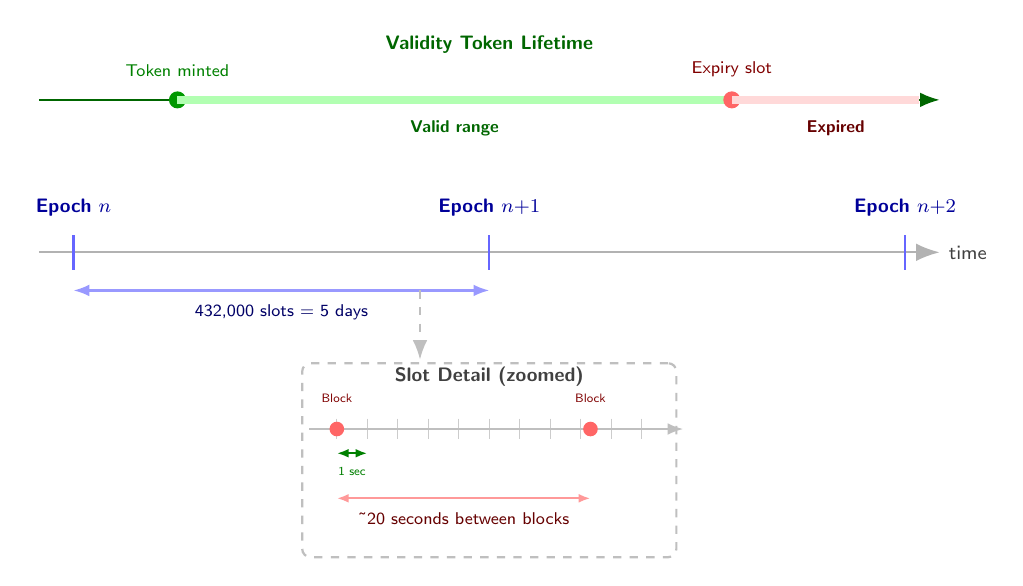
\begin{tikzpicture}[
  scale=0.88,
  every node/.style={transform shape},
]
  % ── Main timeline axis ─────────────────────────────────────────
  \draw[thick, gray!60, -{Latex[length=3mm]}]
    (-6.5, 0) -- (6.5, 0)
    node[right, font=\sffamily\footnotesize, text=gray!50!black] {time};

  % ── Epoch markers ──────────────────────────────────────────────
  \foreach \x/\lab in {-6/Epoch $n$, 0/Epoch $n{+}1$, 6/Epoch $n{+}2$} {
    \draw[thick, blue!60] (\x, -0.25) -- (\x, 0.25);
    \node[font=\sffamily\footnotesize\bfseries, text=blue!60!black,
          above=4pt] at (\x, 0.25) {\lab};
  }

  % 5 days label
  \draw[{Latex[length=2mm]}-{Latex[length=2mm]}, thick, blue!40]
    (-6, -0.55) -- (0, -0.55)
    node[midway, below=2pt, font=\sffamily\scriptsize, text=blue!40!black]
    {432{,}000 slots = 5 days};

  % ── Slot detail (zoomed inset) ─────────────────────────────────
  \node[draw, rounded corners=3pt, thick, dashed, gray!50,
        minimum width=5.4cm, minimum height=2.8cm, fill=white]
    (inset) at (0, -3.0) {};
  \node[font=\sffamily\footnotesize\bfseries, text=gray!50!black]
    at (0, -1.8) {Slot Detail (zoomed)};

  % Slot ticks
  \foreach \i in {0,...,10} {
    \pgfmathsetmacro{\xpos}{-2.2 + \i * 0.44}
    \draw[thin, gray!40] (\xpos, -2.4) -- (\xpos, -2.7);
  }
  \draw[thick, gray!50, -{Latex[length=2mm]}]
    (-2.6, -2.55) -- (2.8, -2.55);

  % 1-second label
  \draw[{Latex[length=1.5mm]}-{Latex[length=1.5mm]}, thick, green!50!black]
    (-2.2, -2.9) -- (-1.76, -2.9)
    node[midway, below=2pt, font=\sffamily\tiny, text=green!50!black]
    {1 sec};

  % Block markers (every ~20 slots)
  \fill[red!60] (-2.2, -2.55) circle (3pt);
  \fill[red!60] (1.46, -2.55) circle (3pt);  % ~slot 8 of 10 shown

  % Block label
  \node[font=\sffamily\tiny, text=red!50!black, above=3pt]
    at (-2.2, -2.4) {Block};
  \node[font=\sffamily\tiny, text=red!50!black, above=3pt]
    at (1.46, -2.4) {Block};

  % ~20s between blocks
  \draw[{Latex[length=1.5mm]}-{Latex[length=1.5mm]}, thick, red!40]
    (-2.2, -3.55) -- (1.46, -3.55)
    node[midway, below=2pt, font=\sffamily\scriptsize, text=red!40!black]
    {\textasciitilde20 seconds between blocks};

  % Arrow from main timeline to inset
  \draw[guidearrow, dashed, gray!50]
    (-1, -0.55) -- (-1, -1.55);

  % ── Validity token timeline ────────────────────────────────────
  \draw[thick, green!40!black, -{Latex[length=2.5mm]}]
    (-6.5, 2.2) -- (6.5, 2.2);
  \node[font=\sffamily\footnotesize, text=green!40!black, above=2pt]
    at (-6.5, 2.2) {};

  % Mint point
  \fill[green!60!black] (-4.5, 2.2) circle (3.5pt);
  \node[font=\sffamily\scriptsize, text=green!50!black, above=6pt]
    at (-4.5, 2.2) {Token minted};

  % Valid range
  \draw[line width=3pt, green!30]
    (-4.5, 2.2) -- (3.5, 2.2);

  % Expiry point
  \fill[red!60] (3.5, 2.2) circle (3.5pt);
  \node[font=\sffamily\scriptsize, text=red!50!black, above=6pt]
    at (3.5, 2.2) {Expiry slot};

  % Expired range
  \draw[line width=3pt, red!15]
    (3.5, 2.2) -- (6.2, 2.2);

  \node[font=\sffamily\scriptsize, text=green!40!black, below=5pt]
    at (-0.5, 2.2) {\textbf{Valid range}};
  \node[font=\sffamily\scriptsize, text=red!40!black, below=5pt]
    at (5.0, 2.2) {\textbf{Expired}};

  % Label
  \node[font=\sffamily\footnotesize\bfseries, text=green!40!black]
    at (0, 3.0) {Validity Token Lifetime};
\end{tikzpicture}
\caption{Cardano's time model. The upper timeline shows a validity token's
lifetime, from minting to slot-based expiry. The middle timeline shows
epochs (5 days each). The inset zooms into individual slots (1 second each)
and blocks (\textasciitilde20-second intervals). Validators check
transaction validity intervals against token expiry slots to enforce
time-bounded credentials.}
\label{fig:time-model}
\end{figure}


% ============================================================================
\section{Transaction Fees}
\label{sec:fees}
% ============================================================================

\subsection{Deterministic Fee Model}

Cardano's fee model is one of its most practically important features
for production systems. Unlike Ethereum, where the cost of a transaction
is determined by a ``gas auction'' (users bid for block space, and
actual costs depend on network congestion at the moment of inclusion),
Cardano uses a \textbf{deterministic, formula-based fee model}:

\[
  \text{fee} = A \times \text{tx\_size (bytes)} + B
\]

where $A$ and $B$ are protocol parameters. At current mainnet values:
\begin{itemize}[nosep]
  \item $A = 44$ lovelace per byte (the ``per-byte coefficient'')
  \item $B = 155{,}381$ lovelace (the ``constant fee''; the minimum fee
    for any transaction)
\end{itemize}

For a typical native script minting transaction of \textasciitilde400
bytes:
\[
  \text{fee} = 44 \times 400 + 155{,}381 = 173{,}181 \text{ lovelace}
  \approx 0.17 \text{ ADA}
\]

This means the \emph{exact fee is known before the transaction is
submitted}. There is no gas estimation, no fee spike due to network
congestion, and no failed transaction that still costs money. You build
the transaction, calculate its serialized size, apply the formula, and
the result is guaranteed. For a credential system handling thousands of
minting and signing operations, this predictability enables precise
budgeting and cost forecasting.

\subsection{Plutus Script Execution Fees}

Transactions that execute Plutus validator scripts incur additional fees
based on two execution resource metrics: \textbf{CPU steps} and
\textbf{memory units}. The Plutus fee formula adds:

\[
  \text{script\_fee} = \text{cpu\_price} \times \text{cpu\_steps}
    + \text{mem\_price} \times \text{mem\_units}
\]

The total transaction fee is the maximum of the size-based fee and the
execution-based fee. For credential system operations:

\begin{itemize}[nosep]
  \item \textbf{Native script operations} (minting, simple transfers):
    \textasciitilde0.17~ADA. No Plutus execution, so only the size-based
    fee applies.
  \item \textbf{Plutus V2 operations} (signature collection, dues
    enforcement, CIP-68 datum updates): \textasciitilde0.3--0.5~ADA.
    The script execution adds CPU and memory costs.
  \item \textbf{Complex Plutus operations} (multi-input finalization
    consuming 5+ UTxOs): \textasciitilde0.5--1.5~ADA. More inputs mean
    more script context for the validator to process.
\end{itemize}

\subsection{Comparison with Ethereum Gas}

The practical difference is dramatic. During high network activity on
Ethereum (e.g., a popular NFT mint), gas prices can spike from a base of
\textasciitilde20~gwei to 500+~gwei, making a \$2 mint cost \$50 or
more. A transaction that fails validation \emph{still consumes gas} on
Ethereum---the user pays for the failed attempt. On Cardano, fee spikes
do not occur because fees depend only on transaction size and script
execution cost, not on network congestion. And because transactions are
validated locally before submission, a malformed transaction never
reaches the chain and costs nothing.

For a licensing board processing hundreds of minting transactions per
day, this difference is not marginal---it is the difference between
predictable operating costs and unpredictable, potentially order-of-magnitude cost variability.


% ============================================================================
\section{Addresses}
\label{sec:addresses}
% ============================================================================

\subsection{Address Types}

A Cardano address is not simply a hash of a public key (as in Bitcoin).
It is a structured data object that encodes multiple pieces of
information. Understanding address construction is important because the
credential system uses address properties to determine wallet roles and
enforce access control.

Cardano defines several address types, three of which are relevant to
credential systems:

\begin{description}[leftmargin=2.8cm, labelwidth=2.6cm]
  \item[Base Address] The most common address type. It contains two
    credential hashes: a \textbf{payment key hash (PKH)} and a
    \textbf{stake key hash (SKH)}. The PKH controls spending (who can
    consume UTxOs at this address), and the SKH controls stake
    delegation (which stake pool receives delegation from this address's
    ADA). Base addresses are used for all licensee and signer wallets in
    the credential system, as they support both transactions and staking
    rewards.

  \item[Enterprise Address] Contains only a payment key hash---no stake
    component. Enterprise addresses cannot delegate stake or receive
    staking rewards. They are useful for script addresses and
    application-specific wallets where staking is irrelevant. The
    credential system's validator script addresses are enterprise
    addresses.

  \item[Pointer Address] Contains a payment key hash and a ``pointer''
    to a stake key registration on the chain (identified by slot, transaction
    index, and certificate index). Pointer addresses are more compact
    than base addresses but are rarely used in practice and are not
    employed in the credential system.
\end{description}

\subsection{Key Hashes: PKH and SKH}

The payment key hash (PKH) and stake key hash (SKH) are both
28-byte Blake2b-224 hashes of the respective verification keys. These
hashes serve as the fundamental identity unit on Cardano:

\begin{itemize}[nosep]
  \item The \textbf{PKH} identifies \emph{who can spend} UTxOs at an
    address. When a validator script checks whether the correct signer
    is depositing tokens, it compares the transaction's signatories
    against the expected PKH in the datum.
  \item The \textbf{SKH} identifies \emph{who controls delegation}. It
    is relevant for staking rewards but does not affect transaction
    authorization.
\end{itemize}

In the credential system, the authority's PKH is embedded in minting
policies (``only the holder of this PKH can mint''), signer PKHs are
recorded in work product datums (``these specific PKHs must deposit
tokens''), and the licensee's PKH is recorded in license metadata for
identity binding.

\subsection{Bech32 Encoding}

Cardano addresses are displayed in \textbf{Bech32} encoding, a
human-readable format that includes an error-detecting checksum. Mainnet
addresses start with \texttt{addr1...} and testnet addresses with
\texttt{addr\_test1...}. The Bech32 encoding ensures that a mistyped
character in an address is detected before a transaction is submitted,
preventing accidental loss of funds. The prefix also prevents
accidentally sending mainnet transactions on the testnet or vice versa.

\begin{figure}[htbp]
\centering
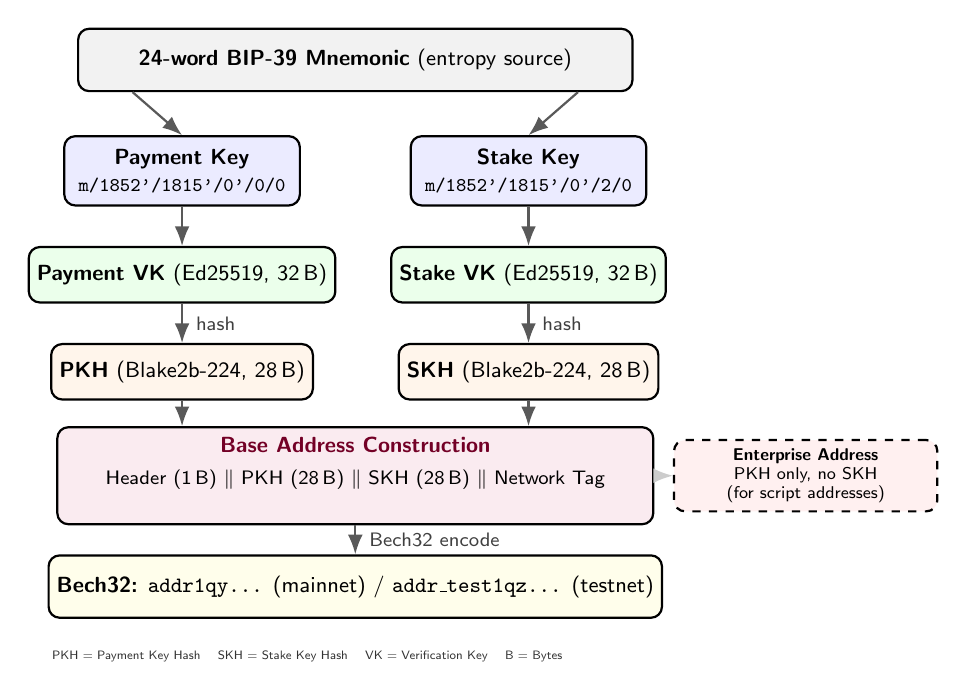
\begin{tikzpicture}[
  scale=0.88,
  every node/.style={transform shape},
]
  % ── Mnemonic at top ────────────────────────────────────────────
  \node[guidebox, fill=gray!10, minimum width=8cm, minimum height=0.9cm]
    (mnemonic) at (0, 5.2)
    {\textbf{24-word BIP-39 Mnemonic} (entropy source)};

  % ── HD Derivation ──────────────────────────────────────────────
  \node[guidebox, fill=blue!8, minimum width=3.4cm, minimum height=1.0cm]
    (paypath) at (-2.5, 3.6)
    {\textbf{Payment Key}\\
     \footnotesize\texttt{m/1852'/1815'/0'/0/0}};
  \node[guidebox, fill=blue!8, minimum width=3.4cm, minimum height=1.0cm]
    (stakepath) at (2.5, 3.6)
    {\textbf{Stake Key}\\
     \footnotesize\texttt{m/1852'/1815'/0'/2/0}};

  \draw[guidearrow] (mnemonic.south west) ++(0.8,0) -- (paypath.north);
  \draw[guidearrow] (mnemonic.south east) ++(-0.8,0) -- (stakepath.north);

  % ── Verification Keys ──────────────────────────────────────────
  \node[guidebox, fill=green!8, minimum width=3.4cm, minimum height=0.8cm]
    (payvk) at (-2.5, 2.1)
    {\textbf{Payment VK} (Ed25519, 32\,B)};
  \node[guidebox, fill=green!8, minimum width=3.4cm, minimum height=0.8cm]
    (stakevk) at (2.5, 2.1)
    {\textbf{Stake VK} (Ed25519, 32\,B)};

  \draw[guidearrow] (paypath.south) -- (payvk.north);
  \draw[guidearrow] (stakepath.south) -- (stakevk.north);

  % ── Hashing ────────────────────────────────────────────────────
  \node[guidebox, fill=orange!8, minimum width=3.4cm, minimum height=0.8cm]
    (pkh) at (-2.5, 0.7)
    {\textbf{PKH} (Blake2b-224, 28\,B)};
  \node[guidebox, fill=orange!8, minimum width=3.4cm, minimum height=0.8cm]
    (skh) at (2.5, 0.7)
    {\textbf{SKH} (Blake2b-224, 28\,B)};

  \draw[guidearrow] (payvk.south) --
    node[right=2pt, guidelabel] {hash} (pkh.north);
  \draw[guidearrow] (stakevk.south) --
    node[right=2pt, guidelabel] {hash} (skh.north);

  % ── Address Assembly ───────────────────────────────────────────
  \node[guidebox, fill=purple!8, minimum width=8.6cm, minimum height=1.4cm]
    (addr) at (0, -0.8) {};
  \node[font=\sffamily\small\bfseries, text=purple!60!black]
    at (0, -0.35) {Base Address Construction};
  \node[font=\sffamily\footnotesize] at (0, -0.85)
    {Header (1\,B) $\|$ PKH (28\,B) $\|$ SKH (28\,B)
     $\|$ Network Tag};

  \draw[guidearrow] (pkh.south) -- (addr.north -| pkh);
  \draw[guidearrow] (skh.south) -- (addr.north -| skh);

  % ── Bech32 Encoding ───────────────────────────────────────────
  \node[guidebox, fill=yellow!8, minimum width=8.6cm, minimum height=0.9cm]
    (bech32) at (0, -2.4)
    {\textbf{Bech32:} \texttt{addr1qy...} (mainnet) /
     \texttt{addr\_test1qz...} (testnet)};

  \draw[guidearrow] (addr.south) --
    node[right=2pt, guidelabel] {Bech32 encode} (bech32.north);

  % ── Enterprise address (side note) ────────────────────────────
  \node[guidebox, fill=red!6, minimum width=3.8cm, minimum height=1.0cm,
        dashed, font=\sffamily\scriptsize]
    (enterprise) at (6.5, -0.8)
    {\textbf{Enterprise Address}\\PKH only, no SKH\\(for script addresses)};

  \draw[guidearrow, dashed, gray!40]
    (addr.east) -- (enterprise.west);

  % ── Legend ─────────────────────────────────────────────────────
  \node[font=\sffamily\tiny, text=gray!40!black, anchor=north west]
    at (-4.5, -3.2)
    {PKH = Payment Key Hash \quad SKH = Stake Key Hash \quad
     VK = Verification Key \quad B = Bytes};
\end{tikzpicture}
\caption{Cardano address construction from mnemonic to Bech32-encoded
address. A 24-word mnemonic seeds HD key derivation (CIP-1852), producing
payment and stake verification keys. Each is hashed with Blake2b-224 to
produce 28-byte key hashes. A base address combines both hashes with a
network tag; an enterprise address uses only the payment key hash.}
\label{fig:address-construction}
\end{figure}


% ============================================================================
\section{UTxO Selection Strategies}
\label{sec:utxo-selection}
% ============================================================================

\subsection{The UTxO Selection Problem}

When building a transaction, you must select which UTxOs to consume as
inputs. This is a non-trivial optimization problem. Consider a licensee
who has received signature tokens in 20 separate transactions, each
creating a separate UTxO. To sign a document (requiring 1 signature
token and 1 validity token), the transaction builder must choose which
UTxO(s) to consume. The choice affects:

\begin{enumerate}[nosep]
  \item \textbf{Transaction size.} Each input adds \textasciitilde40--60
    bytes to the transaction. More inputs mean a larger transaction and
    a higher fee.
  \item \textbf{Change outputs.} If a UTxO contains more value than
    needed, the excess must be returned as a change output, which itself
    requires a minUTxO deposit.
  \item \textbf{UTxO set health.} Poor selection strategies can
    fragment the UTxO set into many tiny outputs, each locking a minUTxO
    deposit, gradually eroding the wallet's effective balance.
  \item \textbf{Transaction size limit.} Cardano enforces a maximum
    transaction size of \textbf{16,384 bytes (16~KB)}. A transaction
    that consumes too many inputs may exceed this limit and fail to
    build.
\end{enumerate}

\subsection{LargestFirstSelector}

The \texttt{LargestFirstSelector} strategy sorts all available UTxOs by
value (largest first) and greedily selects UTxOs until the required
value is covered. This is the default strategy in PyCardano and the one
used by the credential system.

\textbf{Advantages:}
\begin{itemize}[nosep]
  \item Minimizes the number of inputs (and therefore transaction size)
    by preferring large UTxOs.
  \item Produces fewer, larger change outputs, reducing UTxO
    fragmentation over time.
  \item Simple and predictable---the same inputs produce the same
    selection.
\end{itemize}

\textbf{Disadvantages:}
\begin{itemize}[nosep]
  \item Large UTxOs are consumed first, potentially leaving a ``long
    tail'' of small UTxOs that are individually too small to cover
    transaction fees.
  \item Deterministic selection can lead to repeated use of the same
    UTxOs, causing temporary contention in high-throughput scenarios.
\end{itemize}

\subsection{RandomImproveSelector}

The \texttt{RandomImproveSelector} takes a different approach. It first
makes a random initial selection that covers the required value, then
iteratively attempts to improve the selection by swapping UTxOs to
minimize the change output. The goal is to produce a change output as
close to zero as possible, reducing the number of dust UTxOs over time.

\textbf{Advantages:}
\begin{itemize}[nosep]
  \item Distributes UTxO consumption more evenly across the wallet's
    UTxO set, reducing fragmentation over time.
  \item The randomness reduces contention in scenarios where multiple
    transactions are built concurrently (relevant for high-volume
    minting operations).
  \item Tends to produce a healthier UTxO distribution in the long run.
\end{itemize}

\textbf{Disadvantages:}
\begin{itemize}[nosep]
  \item Non-deterministic: building the same transaction twice may
    select different inputs, complicating testing and debugging.
  \item May select more inputs than \texttt{LargestFirstSelector} for a
    given transaction, increasing fees slightly.
\end{itemize}

\subsection{Practical Implications}

For the credential system, UTxO selection strategy matters most during
two operations:

\begin{enumerate}[nosep]
  \item \textbf{Batch minting.} When minting 100 signature tokens for a
    new licensee, the authority wallet must have a UTxO with enough ADA
    to cover fees and the minUTxO deposit. If the authority's ADA is
    fragmented across dozens of small UTxOs, the transaction builder may
    need to consume many inputs, potentially exceeding the 16~KB limit.
  \item \textbf{Token consolidation.} A licensee who has signed many
    documents will have accumulated change UTxOs. Periodic consolidation
    (sending all UTxOs back to oneself in a single transaction) reduces
    the UTxO count and recovers locked minUTxO deposits.
\end{enumerate}

The credential system uses \texttt{LargestFirstSelector} by default
with a 200,000~lovelace fee buffer, switching to
\texttt{RandomImproveSelector} for high-volume operations where
concurrent transaction building might cause contention on the same
large UTxOs.


% ============================================================================
\section{Chapter Summary}
\label{sec:ch2-summary}
% ============================================================================

This chapter has covered the seven architectural pillars of Cardano that
underpin the credential verification system:

\begin{enumerate}[nosep]
  \item \textbf{The eUTxO Model} extends Bitcoin's UTxO with datums
    (data on UTxOs), redeemers (spending arguments), and script context
    (full transaction visibility), enabling deterministic smart contract
    execution.
  \item \textbf{Native Multi-Assets} allow tokens to exist at the
    ledger level without smart contracts, providing the same security
    guarantees as ADA at lower cost.
  \item \textbf{The minUTxO Deposit} prevents ledger bloat by requiring
    a recoverable ADA deposit proportional to UTxO size---a cost that
    must be budgeted but is not consumed.
  \item \textbf{Slots, Epochs, and Time} provide the discrete time
    model that enables slot-based token expiry and time-bounded
    transaction validity.
  \item \textbf{Deterministic Fees} ensure that transaction costs are
    known exactly before submission, enabling precise cost forecasting
    for credential operations.
  \item \textbf{Address Construction} from HD-derived key hashes
    provides the identity primitives (PKH, SKH) used throughout the
    system for access control and credential binding.
  \item \textbf{UTxO Selection Strategies} balance transaction
    efficiency against UTxO set health, with implications for
    high-volume minting and long-term wallet management.
\end{enumerate}

With this architectural foundation in place, Chapter~3 will introduce
the specific token types, minting policies, and smart contracts that
implement the credential verification system on top of these primitives.


% ============================================================================
% CHAPTER 3: Cardano Improvement Proposals (CIPs)
% ============================================================================
% ============================================================================
% Chapter 3: Cardano Improvement Proposals (CIPs)
% Study Guide — Blockchain-Based Credential Verification
% ============================================================================

\chapter{Cardano Improvement Proposals (CIPs)}
\label{ch:cips}

% --- Shared TikZ styles for this chapter ------------------------------------
\tikzset{
  guidebox/.style={draw, rounded corners=4pt, thick, align=center,
    font=\sffamily\small, fill=white, minimum height=1cm},
  guidearrow/.style={-{Latex[length=2.5mm]}, thick, color=gray!70!black},
  guidelabel/.style={font=\sffamily\footnotesize, text=gray!50!black},
}

Cardano's technical evolution is governed by a structured, community-driven
process called the \emph{Cardano Improvement Proposal} (CIP) system.  Every
significant feature---from how wallets derive keys to how smart contracts
reference on-chain data---begins life as a numbered CIP, undergoes public
review, and is either accepted, modified, or rejected before implementation.
Understanding the CIP landscape is essential for anyone building on Cardano
because CIPs define the \emph{interface contracts} that all tools, wallets,
and dApps must honour.

This chapter examines the eight CIPs most relevant to the credential
verification system described in this guide.  We begin with the governance
process itself, then walk through the token metadata standards (CIP-25 and
CIP-68), the wallet connectivity bridge (CIP-30), the Plutus~V2 trio that
made advanced datum handling possible (CIPs~31, 32, and~33), and the
hierarchical deterministic wallet derivation standard (CIP-1852).  For each
CIP we explain \emph{what problem it solves}, \emph{how it works
technically}, and \emph{how the credential system uses it}.


% ============================================================================
\section{What Are CIPs?}
\label{sec:cips-overview}
% ============================================================================

A Cardano Improvement Proposal is a formal design document that describes a
new feature, process, or informational guideline for the Cardano ecosystem.
The CIP process is modelled directly on the Internet Engineering Task Force's
\emph{Request for Comments} (RFC) system and Python's PEP process: anyone may
author a proposal, but acceptance requires community review, editor approval,
and---for protocol-level changes---implementation by the core development
teams at Input Output Global (IOG), the Cardano Foundation, or Emurgo.

CIPs are classified into three categories:

\begin{description}[leftmargin=1.5em, style=nextline]
  \item[Standards Track] Proposals that change the protocol, transaction
    format, validation rules, or networking layer.  Examples include CIP-31
    (Reference Inputs) and CIP-32 (Inline Datums).
  \item[Process] Proposals that change governance procedures, the CIP process
    itself, or tooling requirements.
  \item[Informational] Proposals that document conventions, best practices, or
    design rationale without mandating changes.  CIP-25 (NFT Metadata) began
    as an informational standard that the community adopted voluntarily.
\end{description}

The lifecycle of a CIP proceeds through several stages: \textbf{Draft} (initial
submission to the CIP repository on GitHub), \textbf{Proposed} (editors
confirm the proposal is well-formed), \textbf{Active} (the community has
reached rough consensus and implementations exist), and optionally
\textbf{Inactive} or \textbf{Superseded} if a newer CIP replaces it.

For the credential system, CIPs are not merely background reading---they are
the \emph{specifications} that the code implements.  The minting policy encodes
CIP-25 metadata structures.  The wallet module follows CIP-1852 derivation
paths.  The revocation mechanism depends on CIP-68 datum semantics.
Understanding each CIP at a technical level is prerequisite to understanding
why the system works the way it does.

\begin{figure}[ht]
\centering
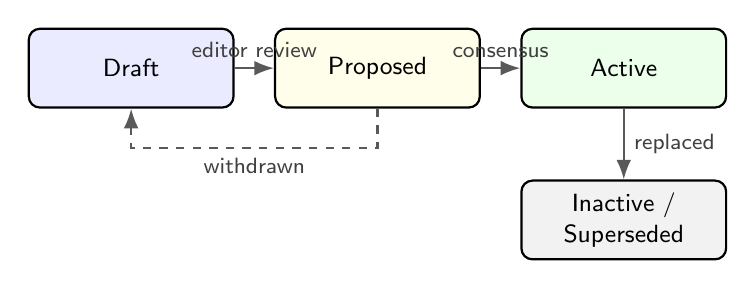
\begin{tikzpicture}[node distance=1.8cm and 0.5cm]
  \node[guidebox, fill=blue!8, minimum width=2.6cm] (draft) {Draft};
  \node[guidebox, fill=yellow!8, minimum width=2.6cm, right=of draft] (proposed) {Proposed};
  \node[guidebox, fill=green!8, minimum width=2.6cm, right=of proposed] (active) {Active};
  \node[guidebox, fill=gray!10, minimum width=2.6cm, below=0.9cm of active] (inactive) {Inactive /\\Superseded};

  \draw[guidearrow] (draft) -- node[above, guidelabel] {editor review} (proposed);
  \draw[guidearrow] (proposed) -- node[above, guidelabel] {consensus} (active);
  \draw[guidearrow] (active) -- node[right, guidelabel] {replaced} (inactive);
  \draw[guidearrow, dashed] (proposed.south) -- ++(0,-0.5) -| node[below, near start, guidelabel] {withdrawn} (draft.south);
\end{tikzpicture}
\caption{CIP lifecycle stages.  A proposal moves from Draft through Proposed
to Active once community consensus is reached and implementations exist.
Proposals may be withdrawn or eventually superseded by newer standards.}
\label{fig:cip-lifecycle}
\end{figure}


% ============================================================================
\section{CIP-25: NFT Metadata Standard}
\label{sec:cip25}
% ============================================================================

\subsection{The Problem}

Cardano's native multi-asset framework allows anyone to mint custom tokens,
but the ledger itself stores only three pieces of information about each
token: the \emph{policy ID} (a Blake2b-224 hash of the minting policy script),
the \emph{asset name} (an arbitrary byte string up to 32~bytes), and the
\emph{quantity}.  There is no built-in mechanism for attaching human-readable
names, images, descriptions, or any other metadata to a token.  Without a
standard, every marketplace, wallet, and explorer would need to negotiate
metadata formats bilaterally---an untenable situation for an open ecosystem.

\subsection{How It Works}

CIP-25 solves this by defining a JSON schema that is embedded in the
\textbf{transaction auxiliary data} (formerly called ``transaction metadata'')
at the time the token is minted.  The auxiliary data is a map keyed by
integer labels; CIP-25 reserves label~\texttt{721} for NFT metadata.

The schema is hierarchical: under label~721, the top-level key is the
\textbf{policy ID} (hex-encoded).  Under each policy ID, keys are
\textbf{asset names} (hex or UTF-8).  Under each asset name, the metadata
object contains at minimum:

\begin{itemize}[nosep]
  \item \texttt{name} --- a human-readable display name
  \item \texttt{image} --- a URI (typically IPFS) pointing to the token's
    image
  \item \texttt{description} --- free-text description
\end{itemize}

Additional fields are permitted and commonly used: \texttt{mediaType},
\texttt{files} (for multi-asset bundles), and arbitrary key-value pairs.
Wallets and marketplaces parse the minting transaction's auxiliary data to
display this information to users.

A critical property of CIP-25 metadata is that it is \textbf{immutable once
written}.  The metadata exists in the auxiliary data of a specific
transaction.  Transactions, once confirmed on-chain, cannot be altered.  This
means that whatever metadata is attached at mint time is the metadata
forever---there is no mechanism within CIP-25 to update, correct, or revoke
the metadata after minting.

For simple NFTs---artwork, collectibles, event tickets---immutability is a
feature.  For credentials that may need to reflect status changes
(revocation, suspension, renewal), immutability is a fundamental limitation.
This limitation is precisely what motivated CIP-68.

\subsection{How the Credential System Uses CIP-25}

In the credential system, CIP-25 metadata is attached to license NFTs at
mint time.  The metadata records the license type, jurisdiction, issue date,
license number, and the licensee's public key hash.  Because this
information is immutable, it serves as a permanent attestation: ``At this
point in time, this authority issued this credential to this individual.''

Verification of the attestation is straightforward: a verifier checks that
(1)~the token exists in the holder's wallet, (2)~the policy ID matches the
known authority, and (3)~the CIP-25 metadata in the minting transaction
matches the claimed credential details.

\begin{figure}[ht]
\centering
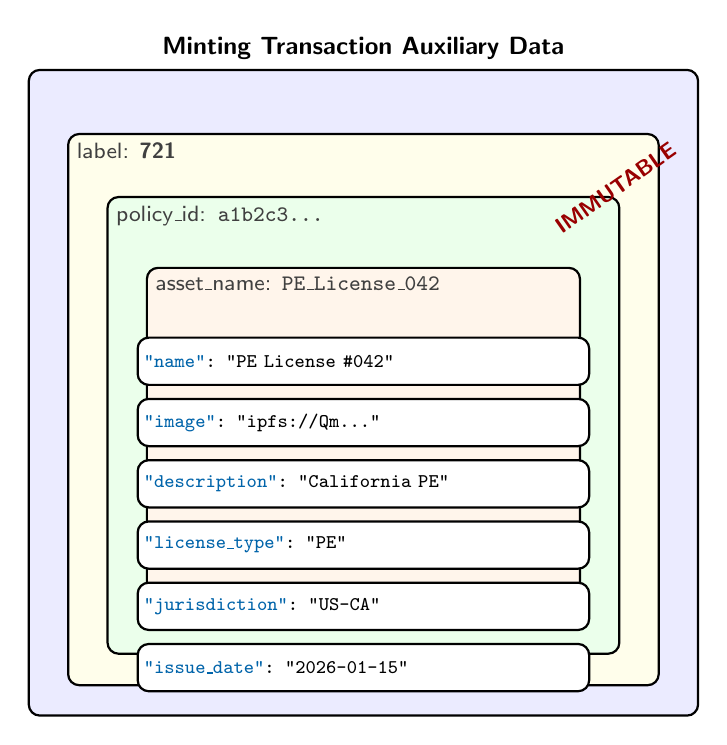
\begin{tikzpicture}[
  metabox/.style={guidebox, text width=5.5cm, align=left,
    font=\ttfamily\scriptsize, minimum height=0.6cm},
]
  % Outer transaction box
  \node[guidebox, fill=blue!8, minimum width=8.5cm, minimum height=8.2cm,
    label={[font=\sffamily\small\bfseries]above:Minting Transaction Auxiliary Data}] (txbox) at (0,0) {};

  % Label 721
  \node[guidebox, fill=yellow!8, minimum width=7.5cm, minimum height=7cm,
    anchor=north] (l721) at (0,3.3) {};
  \node[guidelabel, anchor=north west] at (l721.north west) {label: \textbf{721}};

  % Policy ID
  \node[guidebox, fill=green!8, minimum width=6.5cm, minimum height=5.8cm,
    anchor=north] (pid) at (0,2.5) {};
  \node[guidelabel, anchor=north west, text width=6cm] at (pid.north west)
    {policy\_id: \texttt{a1b2c3...}};

  % Asset name
  \node[guidebox, fill=orange!8, minimum width=5.5cm, minimum height=4.4cm,
    anchor=north] (aname) at (0,1.6) {};
  \node[guidelabel, anchor=north west] at (aname.north west)
    {asset\_name: \texttt{PE\_License\_042}};

  % Fields
  \node[metabox, fill=white] (f1) at (0,0.4)
    {\textcolor{keyword}{"name"}: "PE License \#042"};
  \node[metabox, fill=white, below=0.15cm of f1] (f2)
    {\textcolor{keyword}{"image"}: "ipfs://Qm..."};
  \node[metabox, fill=white, below=0.15cm of f2] (f3)
    {\textcolor{keyword}{"description"}: "California PE"};
  \node[metabox, fill=white, below=0.15cm of f3] (f4)
    {\textcolor{keyword}{"license\_type"}: "PE"};
  \node[metabox, fill=white, below=0.15cm of f4] (f5)
    {\textcolor{keyword}{"jurisdiction"}: "US-CA"};
  \node[metabox, fill=white, below=0.15cm of f5] (f6)
    {\textcolor{keyword}{"issue\_date"}: "2026-01-15"};

  % Immutable label
  \node[font=\sffamily\footnotesize\bfseries, text=red!60!black,
    rotate=35] at (3.2,2.6) {IMMUTABLE};
\end{tikzpicture}
\caption{CIP-25 metadata structure.  The JSON schema is nested under
label~721, then by policy ID and asset name.  Once written to the
transaction auxiliary data, the metadata cannot be changed.}
\label{fig:cip25-metadata}
\end{figure}


% ============================================================================
\section{CIP-68: Datum Metadata Standard}
\label{sec:cip68}
% ============================================================================

CIP-68 is the single most important CIP for the credential verification
system.  It solves the fundamental limitation of CIP-25---immutable
metadata---by introducing a \textbf{dual-token pattern} that separates
ownership from metadata, enabling authority-controlled updates without
requiring access to the token holder's private key.  This section is
intentionally the longest in the chapter because understanding CIP-68 is
prerequisite to understanding how credential revocation works.

\subsection{The Problem CIP-68 Solves}

Consider a professional engineering license issued as a CIP-25 NFT.  The
metadata at mint time includes \texttt{status: active}.  Two years later, the
licensing board discovers misconduct and needs to revoke the license.  Under
CIP-25, this is \emph{impossible on-chain}: the metadata is baked into the
minting transaction and cannot be altered.  The board's only options are:

\begin{enumerate}[nosep]
  \item \textbf{Burn and re-mint.}  The authority could burn the original
    token and mint a new one with \texttt{status: revoked}.  But burning
    requires consuming the UTxO that holds the token---which is in the
    \emph{licensee's} wallet.  Under the eUTxO model, spending a UTxO
    requires the holder's private key.  A revoked licensee has no incentive
    to cooperate, and the authority \emph{cannot} spend the licensee's UTxO
    without that key.
  \item \textbf{Off-chain revocation list.}  The authority maintains a
    database of revoked credentials, and verifiers must check both the
    on-chain token and the off-chain list.  This reintroduces centralized
    infrastructure, single points of failure, and availability dependencies
    ---exactly the problems blockchain was supposed to solve.
  \item \textbf{Accept that on-chain revocation is impossible.}  Many
    early Cardano credential projects reached this conclusion and treated
    the blockchain as a timestamping service only.
\end{enumerate}

CIP-68 provides a fourth option: \textbf{mutable on-chain metadata} through
a clever separation of concerns.

\subsection{The Dual-Token Pattern}

CIP-68 defines a naming convention using \textbf{asset name labels}---a
4-byte prefix prepended to the asset name that identifies the token's role.
The two most important labels are:

\begin{description}[leftmargin=2em, style=nextline, nosep]
  \item[Label 100 --- Reference Token]
    Held by the \textbf{issuing authority}.  This token sits at a script
    address (not a personal wallet) and carries an \textbf{inline datum}
    containing all mutable metadata: license type, jurisdiction, issue date,
    status, and any other fields the authority may need to update.  Because
    the Reference Token is at a script address controlled by the authority,
    the authority can spend and re-create this UTxO with an updated datum at
    any time, without any involvement from the token holder.

  \item[Label 222 --- User Token]
    Held by the \textbf{credential holder} (the licensee).  This token is
    a standard native asset that lives in the holder's personal wallet.  It
    is \emph{immutable} in the CIP-25 sense---the holder possesses it as
    proof of credential issuance.  The User Token contains no mutable
    metadata; its sole purpose is to attest that the holder was issued a
    credential under a specific policy.
\end{description}

The two tokens share the same policy ID and base asset name, differing only
in their 4-byte label prefix.  This creates a cryptographic link: given a
User Token with asset name \texttt{000de140} + \texttt{PE\_License\_042},
anyone can deterministically compute the corresponding Reference Token's
asset name as \texttt{000643b0} + \texttt{PE\_License\_042} and look up its
inline datum to read the current metadata.

\subsection{How Revocation Works}

The breakthrough insight of CIP-68 for credential systems is this: the
authority can \textbf{revoke a credential by updating the Reference Token's
datum} from \texttt{status: active} to \texttt{status: revoked}.  This
operation:

\begin{itemize}[nosep]
  \item Requires \textbf{only the authority's signature} (the Reference Token
    is at the authority's script address).
  \item Does \textbf{not touch the User Token} in the licensee's wallet---the
    authority never needs the licensee's private key.
  \item Propagates \textbf{globally within minutes} (Cardano's finality
    window).
  \item Is \textbf{verifiable by anyone}: read the Reference Token's inline
    datum, check the status field.
  \item Is \textbf{auditable}: the chain of datum updates (active $\to$
    suspended $\to$ revoked) is visible in the transaction history.
\end{itemize}

This is the mechanism that makes eUTxO-based credential revocation possible
without off-chain infrastructure, without the holder's cooperation, and
without burning the original token.

\subsection{Technical Details}

The Reference Token's inline datum follows a standard structure defined by
CIP-68:

\begin{lstlisting}[language={}, caption={CIP-68 datum structure (simplified)}]
{
  "constructor": 0,
  "fields": [
    {                          // metadata map
      "license_type": "PE",
      "jurisdiction": "US-CA",
      "license_number": "PE-2026-00042",
      "issue_date": "2026-01-15",
      "holder_pkh": "abc123...",
      "status": "active",      // <-- MUTABLE
      "last_updated": 12345678 // slot number
    },
    1                          // version number
  ]
}
\end{lstlisting}

The datum is encoded as CBOR (Concise Binary Object Representation) and
stored directly in the UTxO as an inline datum (CIP-32).  The \texttt{status}
field can hold any of: \texttt{active}, \texttt{suspended},
\texttt{revoked}, or \texttt{expired}.  Each status change creates a new
transaction on-chain, providing a complete audit trail.

The script address holding the Reference Token enforces that only the
authority's key can spend (and re-create) the UTxO.  This is typically
implemented as a simple \texttt{ScriptPubkey} validator or a Plutus V2
spending validator that checks for the authority's signature in the
transaction signatories.

\subsection{Verification Flow}

When a verifier wants to check a credential, the process is:

\begin{enumerate}[nosep]
  \item Observe the User Token (label~222) in the holder's wallet.
  \item Extract the policy ID and base asset name.
  \item Compute the Reference Token (label~100) asset name.
  \item Query the blockchain for the UTxO containing the Reference Token.
  \item Read the inline datum from that UTxO.
  \item Check the \texttt{status} field.
\end{enumerate}

This entire process requires only standard blockchain queries---no off-chain
service, no authority server, no API key.  The data is public, the datum is
inline (CIP-32), and the verification is purely mathematical.

\begin{figure}[ht]
\centering
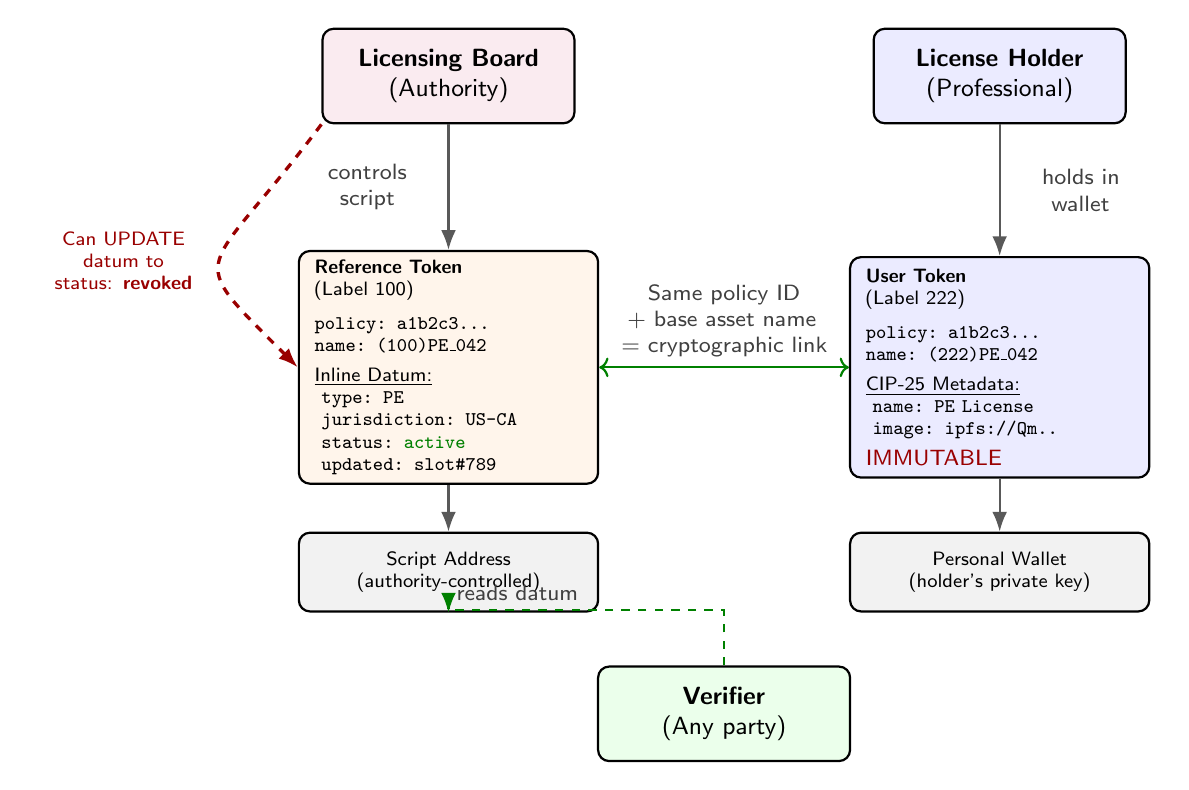
\begin{tikzpicture}[
  entity/.style={guidebox, minimum width=3.2cm, minimum height=1.2cm},
  token/.style={guidebox, minimum width=3.8cm, minimum height=2.8cm,
    text width=3.4cm, align=left, font=\sffamily\scriptsize},
  node distance=1.2cm and 2.8cm,
]
  % --- Entities ---
  \node[entity, fill=purple!8] (authority) at (-3.5, 5.5)
    {\textbf{Licensing Board}\\(Authority)};
  \node[entity, fill=blue!8] (holder) at (3.5, 5.5)
    {\textbf{License Holder}\\(Professional)};

  % --- Reference Token ---
  \node[token, fill=orange!8] (reftok) at (-3.5, 1.8)
    {\textbf{Reference Token}\\(Label 100)\\[4pt]
    \texttt{policy: a1b2c3...}\\
    \texttt{name: (100)PE\_042}\\[3pt]
    \underline{Inline Datum:}\\
    \texttt{\ type: PE}\\
    \texttt{\ jurisdiction: US-CA}\\
    \texttt{\ status: \textcolor{green!50!black}{active}}\\
    \texttt{\ updated: slot\#789}};

  % --- User Token ---
  \node[token, fill=blue!8] (usertok) at (3.5, 1.8)
    {\textbf{User Token}\\(Label 222)\\[4pt]
    \texttt{policy: a1b2c3...}\\
    \texttt{name: (222)PE\_042}\\[3pt]
    \underline{CIP-25 Metadata:}\\
    \texttt{\ name: PE License}\\
    \texttt{\ image: ipfs://Qm..}\\[3pt]
    \footnotesize\textcolor{red!60!black}{IMMUTABLE}};

  % --- Script address ---
  \node[guidebox, fill=gray!10, minimum width=3.8cm, font=\sffamily\scriptsize]
    (script) at (-3.5, -0.8) {Script Address\\(authority-controlled)};

  % --- Personal wallet ---
  \node[guidebox, fill=gray!10, minimum width=3.8cm, font=\sffamily\scriptsize]
    (wallet) at (3.5, -0.8) {Personal Wallet\\(holder's private key)};

  % --- Arrows: ownership ---
  \draw[guidearrow] (authority) -- node[left, guidelabel, text width=1.8cm, align=center]
    {controls\\script} (reftok);
  \draw[guidearrow] (holder) -- node[right, guidelabel, text width=1.8cm, align=center]
    {holds in\\wallet} (usertok);
  \draw[guidearrow] (reftok) -- (script);
  \draw[guidearrow] (usertok) -- (wallet);

  % --- Update arrow ---
  \draw[guidearrow, color=red!60!black, very thick, dashed]
    (authority.south west) .. controls +(-1.5,-2) and +(-1.5,1.5) ..
    node[left, font=\sffamily\scriptsize, text=red!60!black, text width=2.2cm, align=center]
      {Can UPDATE\\datum to\\status: \textbf{revoked}}
    (reftok.west);

  % --- Link arrow ---
  \draw[guidearrow, color=green!50!black, <->]
    (reftok.east) -- node[above, guidelabel, text width=2.8cm, align=center]
      {Same policy ID\\+ base asset name\\= cryptographic link}
    (usertok.west);

  % --- Verifier ---
  \node[entity, fill=green!8] (verifier) at (0, -2.6)
    {\textbf{Verifier}\\(Any party)};
  \draw[guidearrow, dashed, color=green!50!black]
    (verifier.north) -- ++(0,0.7) -- ++(-3.5,0)
    node[above, near end, guidelabel] {reads datum}
    -- (script.south);
\end{tikzpicture}
\caption{CIP-68 dual-token pattern for credential management.  The authority
controls the Reference Token (label~100) at a script address and can update
its inline datum---including the status field---at any time.  The holder
possesses the immutable User Token (label~222) in their personal wallet.
A verifier reads the Reference Token's datum to determine current credential
status.  The authority never needs the holder's private key to revoke.}
\label{fig:cip68-dual-token}
\end{figure}

\subsection{CIP-25 vs.\ CIP-68: Comparison}

Table~\ref{tab:cip25-vs-cip68} summarizes the key differences between the
two metadata standards.  For the credential system, CIP-68's mutable datum
is the enabling feature that makes on-chain revocation practical.

\begin{table}[ht]
\centering
\caption{Comparison of CIP-25 and CIP-68 metadata standards}
\label{tab:cip25-vs-cip68}
\small
\begin{tabular}{@{}p{3.2cm}p{4.8cm}p{4.8cm}@{}}
\toprule
\textbf{Property} & \textbf{CIP-25} & \textbf{CIP-68} \\
\midrule
Metadata location & Transaction auxiliary data (label~721) & Inline datum on Reference Token UTxO \\
Mutability & \textbf{Immutable} --- written once at mint & \textbf{Mutable} --- authority can update datum \\
Token count & 1 token per credential & 2 tokens: Reference (100) + User (222) \\
Who holds metadata & Embedded in minting tx (no custodian) & Reference Token at authority script address \\
Revocation & Not possible on-chain & Datum update: \texttt{status $\to$ revoked} \\
Authority key needed & Only at mint time & At mint \emph{and} for every datum update \\
Holder key needed & Only to transfer/burn the token & Only to transfer/burn the User Token \\
On-chain cost & $\sim$0.2~ADA (single token mint) & $\sim$0.4~ADA (two tokens + datum) \\
Reading metadata & Parse minting tx auxiliary data & Read inline datum from Reference UTxO \\
Audit trail & Single minting event & Full history of datum updates on-chain \\
Requires CIP-31 & No & Yes (reference inputs for reading datum) \\
Requires CIP-32 & No & Yes (inline datums for storing datum) \\
\bottomrule
\end{tabular}
\end{table}

\subsection{Why CIP-68 Matters for Credentials}

The importance of CIP-68 for the credential system cannot be overstated.
Before CIP-68, any Cardano-based credential project faced an impossible
trilemma: (1)~you could store metadata on-chain but it was immutable; (2)~you
could store metadata off-chain but that reintroduced centralization; or
(3)~you could accept that revocation was not truly decentralized.

CIP-68 breaks this trilemma by enabling \textbf{mutable on-chain metadata
under authority control}.  The result is a system where:

\begin{itemize}[nosep]
  \item Credential issuance is on-chain and cryptographically verifiable.
  \item Credential status is on-chain and always current.
  \item Revocation is unilateral by the authority---no holder cooperation
    required.
  \item Verification is fully decentralized---any node can read the datum.
  \item The audit trail is immutable---every status change is a new
    transaction.
\end{itemize}

The dual-token pattern also provides a natural separation between
\emph{proof of issuance} (the User Token in the holder's wallet says ``this
authority issued me a credential'') and \emph{current status} (the Reference
Token's datum says ``the credential is currently active/revoked/suspended'').
This separation mirrors real-world credential systems where a paper
certificate proves issuance but a database query confirms current status---
except that in the CIP-68 model, both proofs are on-chain.


% ============================================================================
\section{CIP-30: dApp--Wallet Web Bridge}
\label{sec:cip30}
% ============================================================================

\subsection{The Problem}

A web-based credential management application needs to interact with a
user's Cardano wallet: reading their address, checking token balances,
and---most critically---asking the wallet to sign transactions.  Without a
standard API, every wallet (Eternl, Nami, Lace, Flint, Typhon, etc.) would
expose its own proprietary JavaScript interface, forcing dApp developers to
write wallet-specific code and creating fragmentation across the ecosystem.

More importantly, the security model must be \textbf{non-custodial}: the
dApp must \emph{never} see the user's private keys.  If the application
server were compromised, an attacker with access to private keys could drain
wallets, forge signatures, or transfer credentials.  The wallet must sign
transactions locally and return only the signed transaction to the dApp.

\subsection{How It Works}

CIP-30 defines a JavaScript API that Cardano wallets inject into the
browser's \texttt{window.cardano} namespace.  The API follows a two-phase
pattern:

\begin{enumerate}[nosep]
  \item \textbf{Discovery and Connection.}  The dApp checks
    \texttt{window.cardano} for available wallets, then calls
    \texttt{cardano.<wallet>.enable()} to request user authorization.  The
    user sees a popup in their wallet extension asking whether to connect.
    If approved, the wallet returns an API handle.
  \item \textbf{Interaction.}  The dApp uses the API handle to call
    methods such as \texttt{getUsedAddresses()},
    \texttt{getUtxos()}, \texttt{getBalance()}, and---most
    importantly---\texttt{signTx(tx, partialSign)}.  The
    \texttt{signTx} method takes an unsigned transaction (CBOR-encoded),
    displays it to the user for approval, signs it with the wallet's private
    key, and returns the signature (or signed transaction).
\end{enumerate}

The critical security property is that the private key \emph{never leaves
the wallet extension}.  The dApp constructs the transaction, but the wallet
signs it.  This is analogous to how a hardware wallet works: the application
builds the transaction, the device signs it, and the application never sees
the signing key.

\subsection{How the Credential System Uses CIP-30}

In the credential system, licensees and signers connect their wallets via
CIP-30 to the web dashboard.  When a professional needs to sign a document
(depositing signature and validity tokens into the work product validator),
the application:

\begin{enumerate}[nosep]
  \item Builds the transaction off-chain using PyCardano (or a JavaScript
    library in the browser).
  \item Sends the unsigned transaction CBOR to the wallet via
    \texttt{signTx()}.
  \item The wallet displays the transaction details (tokens being sent,
    destination address, fee) and asks the user to confirm.
  \item The user approves; the wallet signs and returns the witness.
  \item The application attaches the witness and submits the transaction to
    the network.
\end{enumerate}

At no point does the application server have access to the user's signing
key.  Even if the server is compromised, the attacker cannot sign
transactions on behalf of users.  This non-custodial model is essential for
a credential system where users must maintain sovereign control over their
professional identities.

\begin{figure}[ht]
\centering
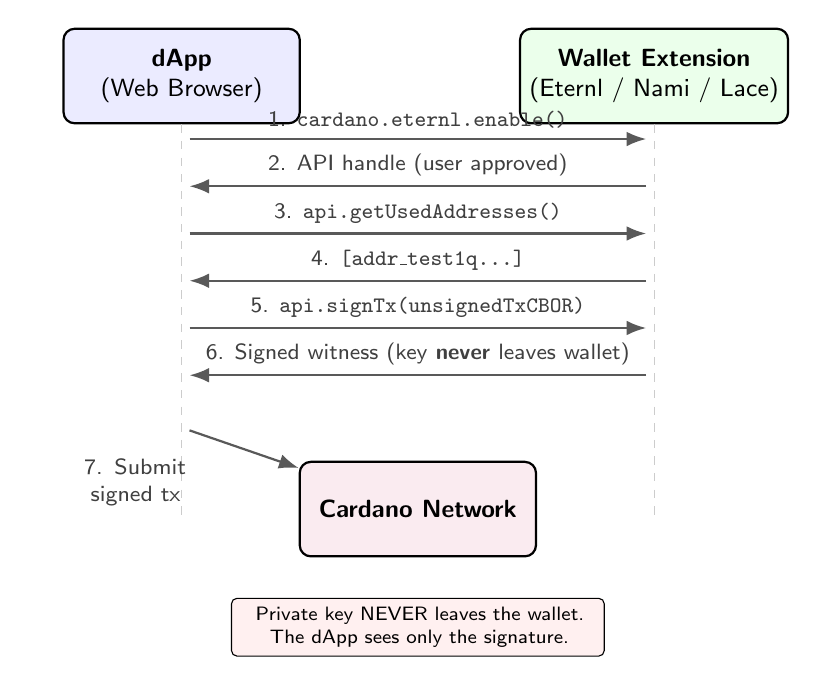
\begin{tikzpicture}[
  actor/.style={guidebox, minimum width=3cm, minimum height=1.2cm},
  node distance=1.5cm and 4.5cm,
]
  % Actors
  \node[actor, fill=blue!8] (dapp) at (0,0) {\textbf{dApp}\\(Web Browser)};
  \node[actor, fill=green!8] (wallet) at (6,0) {\textbf{Wallet Extension}\\(Eternl / Nami / Lace)};
  \node[actor, fill=purple!8] (chain) at (3,-5.5) {\textbf{Cardano Network}};

  % Lifelines
  \draw[dashed, gray!40] (dapp.south) -- ++(0,-5);
  \draw[dashed, gray!40] (wallet.south) -- ++(0,-5);

  % Interactions
  \draw[guidearrow] (0.1,-0.8) -- node[above, guidelabel]
    {1. \texttt{cardano.eternl.enable()}} (5.9,-0.8);
  \draw[guidearrow] (5.9,-1.4) -- node[above, guidelabel]
    {2. API handle (user approved)} (0.1,-1.4);
  \draw[guidearrow] (0.1,-2.0) -- node[above, guidelabel]
    {3. \texttt{api.getUsedAddresses()}} (5.9,-2.0);
  \draw[guidearrow] (5.9,-2.6) -- node[above, guidelabel]
    {4. \texttt{[addr\_test1q...]}} (0.1,-2.6);
  \draw[guidearrow] (0.1,-3.2) -- node[above, guidelabel]
    {5. \texttt{api.signTx(unsignedTxCBOR)}} (5.9,-3.2);
  \draw[guidearrow] (5.9,-3.8) -- node[above, guidelabel]
    {6. Signed witness (key \textbf{never} leaves wallet)} (0.1,-3.8);
  \draw[guidearrow] (0.1,-4.5) -- node[below left, guidelabel, text width=2.5cm, align=center]
    {7. Submit\\signed tx} (chain);

  % Security note
  \node[draw, rounded corners=2pt, fill=red!6, font=\sffamily\scriptsize,
    text width=4.5cm, align=center] at (3,-7)
    {Private key NEVER leaves the wallet.\\The dApp sees only the signature.};
\end{tikzpicture}
\caption{CIP-30 dApp--Wallet interaction flow.  The web application requests
connection, reads addresses and UTxOs, and sends unsigned transactions to the
wallet for signing.  The wallet extension holds the private key locally and
returns only the cryptographic witness.  The dApp never has access to the
signing key.}
\label{fig:cip30-flow}
\end{figure}


% ============================================================================
\section{CIP-31: Reference Inputs}
\label{sec:cip31}
% ============================================================================

\subsection{The Problem}

In the original eUTxO model, every UTxO referenced by a transaction is
\textbf{consumed} (spent).  If a transaction needs to read data from a UTxO
---for example, checking a CIP-68 Reference Token's datum to verify a
credential's status---it must spend that UTxO and recreate it in the same
transaction.  This creates three problems:

\begin{enumerate}[nosep]
  \item \textbf{Concurrency.}  If two transactions both need to read the
    same Reference Token datum, they both try to spend the same UTxO.  Only
    one can succeed; the other fails with a UTxO conflict.  For a credential
    that many parties may verify simultaneously, this is unacceptable.
  \item \textbf{Complexity.}  The spending transaction must include the
    script that guards the UTxO, a redeemer, and must recreate the UTxO with
    exactly the same value and datum---adding transaction size, fees, and
    potential for bugs.
  \item \textbf{Authorization.}  Spending a UTxO requires satisfying its
    spending conditions (e.g., the authority's signature).  A verifier who
    merely wants to \emph{read} the datum should not need the authority's
    key.
\end{enumerate}

\subsection{How It Works}

CIP-31 introduces \textbf{reference inputs}: a new transaction field that
allows a transaction to \emph{read} a UTxO without consuming it.  The UTxO
remains untouched on the ledger after the transaction is processed.  The
transaction's scripts can access the reference input's value, datum, and
address, but the UTxO is not spent.

This is a Plutus~V2 feature introduced in the Vasil hard fork.  In the
transaction body, reference inputs are listed in a separate field
(\texttt{reference\_inputs}) distinct from regular inputs (\texttt{inputs}).
The ledger validates that each referenced UTxO exists at the time the
transaction is processed but does not remove it from the UTxO set.

\subsection{How the Credential System Uses CIP-31}

CIP-31 is critical for the credential system's verification flow.  When a
verifier or a smart contract needs to check a license's current status, the
transaction includes the CIP-68 Reference Token UTxO as a \textbf{reference
input}.  The script reads the inline datum, checks the \texttt{status} field,
and proceeds---all without spending the Reference Token.

This means:
\begin{itemize}[nosep]
  \item Multiple verifications can happen simultaneously (no UTxO contention).
  \item The verifier does not need the authority's key.
  \item The Reference Token UTxO remains stable on-chain.
  \item Transaction size is smaller (no need to recreate the UTxO).
\end{itemize}

Without CIP-31, the CIP-68 pattern would be impractical for any credential
that is verified frequently, because each verification would compete to spend
the same Reference Token UTxO.

\begin{figure}[ht]
\centering
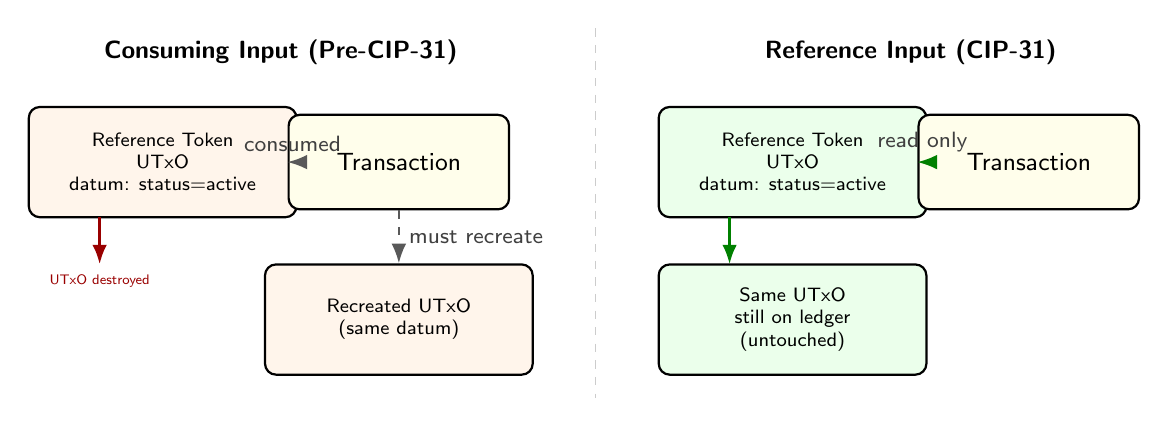
\begin{tikzpicture}[
  utxo/.style={guidebox, minimum width=3.4cm, minimum height=1.4cm,
    font=\sffamily\scriptsize},
  tx/.style={guidebox, fill=yellow!8, minimum width=2.8cm, minimum height=1.2cm},
  node distance=0.8cm and 2.2cm,
]
  % --- Consuming (old way) ---
  \node[font=\sffamily\small\bfseries] at (-4.5,4.2) {Consuming Input (Pre-CIP-31)};

  \node[utxo, fill=orange!8] (utxo1) at (-6,2.8) {Reference Token\\UTxO\\datum: status=active};
  \node[tx] (tx1) at (-3,2.8) {Transaction};
  \node[utxo, fill=orange!8] (utxo1b) at (-3,0.8) {Recreated UTxO\\(same datum)};

  \draw[guidearrow] (utxo1) -- node[above, guidelabel] {consumed} (tx1);
  \draw[guidearrow, dashed] (tx1) -- node[right, guidelabel] {must recreate} (utxo1b);
  \draw[-{Latex[length=2.5mm]}, very thick, red!60!black]
    (-6.8,2.1) -- (-6.8,1.5) node[below, font=\sffamily\tiny, text=red!60!black]
    {UTxO destroyed};

  % --- Reference Input (CIP-31) ---
  \node[font=\sffamily\small\bfseries] at (3.5,4.2) {Reference Input (CIP-31)};

  \node[utxo, fill=green!8] (utxo2) at (2,2.8) {Reference Token\\UTxO\\datum: status=active};
  \node[tx] (tx2) at (5,2.8) {Transaction};

  \draw[guidearrow, dashed, color=green!50!black] (utxo2) --
    node[above, guidelabel] {read only} (tx2);
  \draw[-{Latex[length=2.5mm]}, very thick, green!50!black]
    (1.2,2.1) -- (1.2,1.5) node[below, font=\sffamily\tiny, text=green!50!black]
    {UTxO survives};

  \node[utxo, fill=green!8] (utxo2b) at (2,0.8) {Same UTxO\\still on ledger\\(untouched)};

  % Divider
  \draw[dashed, gray!40] (-0.5,4.5) -- (-0.5,-0.2);
\end{tikzpicture}
\caption{CIP-31 reference inputs compared to consuming inputs.  On the left,
the pre-CIP-31 approach: reading a datum requires consuming the UTxO and
recreating it (expensive, causes contention).  On the right, CIP-31: the
transaction reads the UTxO without consuming it---the UTxO survives
untouched, enabling concurrent reads by multiple transactions.}
\label{fig:cip31-reference-inputs}
\end{figure}


% ============================================================================
\section{CIP-32: Inline Datums}
\label{sec:cip32}
% ============================================================================

\subsection{The Problem}

Before CIP-32, the eUTxO model supported attaching data to script-locked
UTxOs through \textbf{datum hashes}.  When creating a UTxO at a script
address, the transaction included only the \emph{hash} of the datum in the
UTxO itself.  The actual datum content had to be provided separately: either
embedded elsewhere in the transaction's witness set, or stored entirely
off-chain and supplied by whoever eventually spent the UTxO.

This design had two major consequences:

\begin{enumerate}[nosep]
  \item \textbf{Off-chain burden.}  The party spending the UTxO had to know
    the original datum and include it in their spending transaction.  This
    required off-chain coordination: the datum had to be stored somewhere
    (a database, IPFS, a centralized service) and communicated to the
    spender.  If the datum was lost, the UTxO became unspendable.
  \item \textbf{No public readability.}  A third party observing the chain
    could see that a UTxO had a datum hash, but could not determine the
    datum's contents without access to the original data.  This made on-chain
    data effectively opaque to verifiers who had not participated in the
    original transaction.
\end{enumerate}

For a credential system where \emph{any party} must be able to read a
credential's current status, datum hashes are fundamentally inadequate.  A
verifier cannot check \texttt{status: active} if they can only see
\texttt{datum\_hash: 0x3f7a...}.

\subsection{How It Works}

CIP-32 introduces \textbf{inline datums}: the full datum content is stored
\emph{directly in the UTxO} on the ledger.  Any node, wallet, or explorer
that can read the UTxO can also read the datum---no off-chain lookup
required, no special access, no coordination with the datum creator.

Technically, a UTxO's datum field now supports three states:
\begin{description}[nosep, leftmargin=1.5em]
  \item[None] No datum attached (standard ADA-only UTxO).
  \item[Datum Hash] Only the hash is stored on-chain (pre-CIP-32 behavior).
  \item[Inline Datum] The full datum is stored on-chain (CIP-32).
\end{description}

The trade-off is that inline datums increase the UTxO's size on the ledger
and therefore increase the minimum ADA required (minUTxO) to hold the UTxO.
For a credential datum containing license type, jurisdiction, status, and a
few additional fields, the size increase is modest (a few hundred bytes),
and the minUTxO impact is approximately 0.2--0.5~ADA additional.

\subsection{How the Credential System Uses CIP-32}

CIP-32 is what makes CIP-68 \emph{possible}.  The CIP-68 Reference Token
stores its metadata as an inline datum so that:

\begin{itemize}[nosep]
  \item Any verifier can read the credential status by querying the UTxO.
  \item No off-chain service is needed to resolve datum hashes.
  \item Smart contracts executing on-chain (e.g., the Signature Collection
    Validator) can read the Reference Token's datum via reference inputs
    (CIP-31) and make validation decisions based on the credential's current
    status.
\end{itemize}

Without inline datums, the dual-token pattern would require an off-chain
datum registry---reintroducing exactly the centralized infrastructure that
the blockchain architecture is designed to eliminate.  CIP-32, together with
CIP-31, forms the technical foundation upon which CIP-68's mutable on-chain
metadata is built.


% ============================================================================
\section{CIP-33: Reference Scripts}
\label{sec:cip33}
% ============================================================================

\subsection{The Problem}

Plutus scripts (smart contracts) can be large.  A compiled Plutus~V2 script
may be 5--15~KB of serialized CBOR.  Before CIP-33, every transaction that
invoked a Plutus script had to include the \emph{entire compiled script} in
its witness set.  For a credential system where every signing operation
invokes the Signature Collection Validator, this means attaching the same
multi-kilobyte script to every transaction---wasting block space, increasing
fees, and potentially pushing transactions over the 16,384-byte maximum
transaction size.

\subsection{How It Works}

CIP-33 allows a Plutus script to be \textbf{deployed once to a UTxO} and
then \textbf{referenced} by subsequent transactions.  The deployment
transaction creates a UTxO containing the script in a special
\texttt{reference\_script} field.  Future transactions that need to execute
the script include only a reference to this UTxO (its transaction hash and
output index), not the script itself.

The ledger resolves the reference at validation time: when processing a
transaction that references a script UTxO, the node fetches the script from
the referenced UTxO and uses it for validation.  The referenced UTxO is
\emph{not consumed}---like CIP-31 reference inputs, the script UTxO
persists on-chain and can be referenced by unlimited future transactions.

\subsection{How the Credential System Uses CIP-33}

The credential system deploys the Signature Collection Validator and the
Dues Enforcement Contract as reference scripts.  This provides three
benefits:

\begin{enumerate}[nosep]
  \item \textbf{Smaller transactions.}  Signing transactions include only a
    32-byte reference (transaction hash) plus an index, instead of a
    multi-kilobyte script.  This can reduce transaction size by 80--90\%.
  \item \textbf{Lower fees.}  Cardano transaction fees are proportional to
    transaction size.  Smaller transactions mean lower fees for every
    signing operation.
  \item \textbf{Auditability.}  The script is deployed once at a known UTxO.
    Anyone can inspect the exact validator code that governs the credential
    system by reading this single UTxO.
\end{enumerate}

\begin{figure}[ht]
\centering
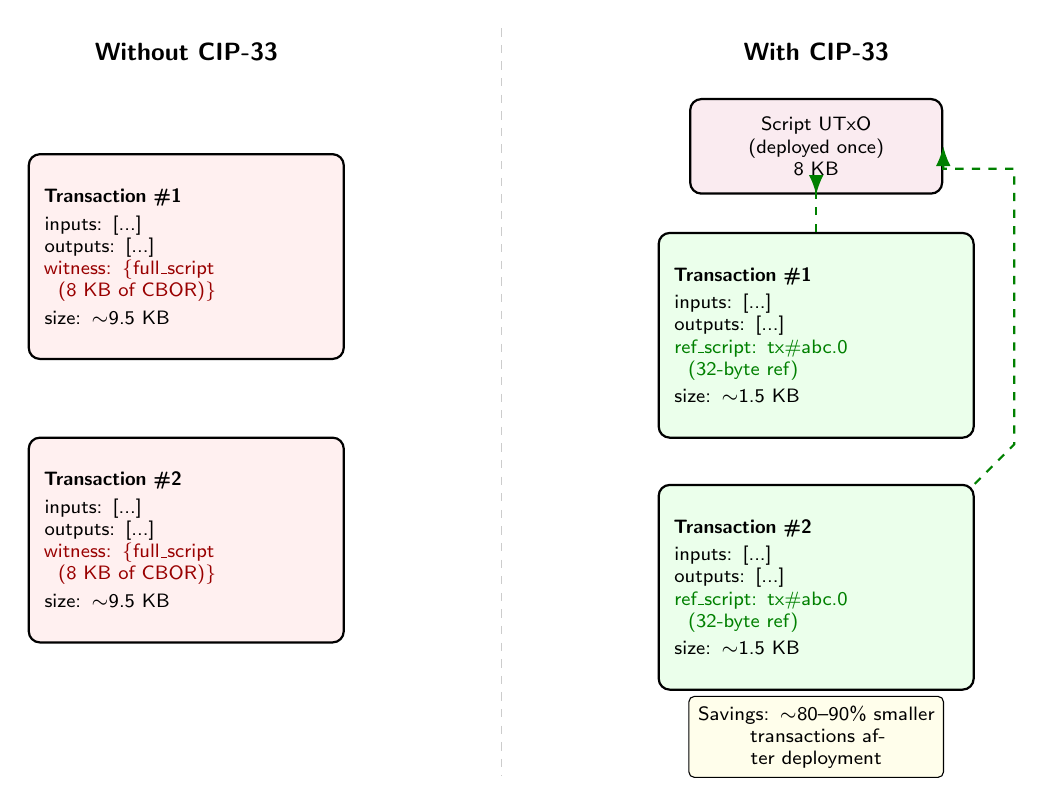
\begin{tikzpicture}[
  txbox/.style={guidebox, minimum width=4cm, minimum height=2.6cm,
    text width=3.6cm, align=left, font=\sffamily\scriptsize},
  scriptbox/.style={guidebox, fill=purple!8, minimum width=3.2cm,
    minimum height=1.2cm, font=\sffamily\scriptsize},
]
  % --- Without CIP-33 ---
  \node[font=\sffamily\small\bfseries] at (-4.5,4.2)
    {Without CIP-33};

  \node[txbox, fill=red!6] (tx1) at (-4.5,1.6)
    {\textbf{Transaction \#1}\\[2pt]
     inputs: [...]\\
     outputs: [...]\\
     \textcolor{red!60!black}{witness: \{full\_script}\\
     \textcolor{red!60!black}{\ \ (8 KB of CBOR)\}}\\[2pt]
     size: $\sim$9.5 KB};

  \node[txbox, fill=red!6] (tx2) at (-4.5,-2)
    {\textbf{Transaction \#2}\\[2pt]
     inputs: [...]\\
     outputs: [...]\\
     \textcolor{red!60!black}{witness: \{full\_script}\\
     \textcolor{red!60!black}{\ \ (8 KB of CBOR)\}}\\[2pt]
     size: $\sim$9.5 KB};

  % --- With CIP-33 ---
  \node[font=\sffamily\small\bfseries] at (3.5,4.2)
    {With CIP-33};

  \node[scriptbox] (deploy) at (3.5,3)
    {Script UTxO\\(deployed once)\\8 KB};

  \node[txbox, fill=green!8] (tx3) at (3.5,0.6)
    {\textbf{Transaction \#1}\\[2pt]
     inputs: [...]\\
     outputs: [...]\\
     \textcolor{green!50!black}{ref\_script: tx\#abc.0}\\
     \textcolor{green!50!black}{\ \ (32-byte ref)}\\[2pt]
     size: $\sim$1.5 KB};

  \node[txbox, fill=green!8] (tx4) at (3.5,-2.6)
    {\textbf{Transaction \#2}\\[2pt]
     inputs: [...]\\
     outputs: [...]\\
     \textcolor{green!50!black}{ref\_script: tx\#abc.0}\\
     \textcolor{green!50!black}{\ \ (32-byte ref)}\\[2pt]
     size: $\sim$1.5 KB};

  % Arrows
  \draw[guidearrow, dashed, color=green!50!black]
    (tx3.north) -- ++(0,0.5) -| (deploy.south);
  \draw[guidearrow, dashed, color=green!50!black]
    (tx4.north east) -- ++(0.5,0.5) -- ++(0,3.5) -| (deploy.east);

  % Savings annotation
  \node[draw, rounded corners=2pt, fill=yellow!8, font=\sffamily\scriptsize,
    text width=3cm, align=center] at (3.5,-4.5)
    {Savings: $\sim$80--90\% smaller\\transactions after deployment};

  % Divider
  \draw[dashed, gray!40] (-0.5,4.5) -- (-0.5,-5);
\end{tikzpicture}
\caption{CIP-33 reference scripts.  Without CIP-33 (left), every transaction
must include the full compiled Plutus script in its witness set, consuming
kilobytes of space per transaction.  With CIP-33 (right), the script is
deployed once to a UTxO, and subsequent transactions reference it with a
compact 32-byte pointer.  Transaction size drops by 80--90\%.}
\label{fig:cip33-reference-scripts}
\end{figure}


% ============================================================================
\section{CIP-1852 / BIP-44: HD Wallet Derivation}
\label{sec:cip1852}
% ============================================================================

\subsection{The Problem}

A naive approach to key management would generate a single random private
key and derive a single address from it.  This creates several problems:

\begin{enumerate}[nosep]
  \item \textbf{No backup recoverability.}  If the key file is lost, all
    funds and credentials are permanently inaccessible.  There is no way to
    regenerate the key.
  \item \textbf{Privacy.}  Using a single address for all transactions
    creates a complete, publicly visible transaction graph.  Every
    credential, every payment, every interaction is linked.
  \item \textbf{Key management complexity.}  If a user needs separate keys
    for different purposes (payment, staking, multiple credentials), they
    must manage multiple independent keys with independent backups.
  \item \textbf{No standard.}  Without a derivation convention, every wallet
    would generate keys differently, making wallet recovery across different
    software impossible.
\end{enumerate}

\subsection{How It Works}

CIP-1852 defines Cardano's \textbf{hierarchical deterministic (HD) wallet}
derivation scheme, building on the BIP-32 (key derivation), BIP-39
(mnemonic encoding), and BIP-44 (multi-account structure) standards from the
Bitcoin ecosystem.

The core idea is that a single \textbf{24-word mnemonic phrase} (BIP-39)
encodes a master seed from which an unlimited number of keys can be derived
deterministically.  Given the same mnemonic, any compliant wallet software
will derive exactly the same keys in exactly the same order.  This means:

\begin{itemize}[nosep]
  \item \textbf{Backup is trivial.}  Write down 24 words.  That is the
    complete backup for all current and future keys.
  \item \textbf{Recovery works across wallets.}  Import the mnemonic into
    Eternl, Nami, Lace, or any CIP-1852-compliant wallet, and all keys are
    regenerated identically.
  \item \textbf{Unlimited addresses.}  Increment the index in the derivation
    path to generate fresh addresses for privacy.
\end{itemize}

\subsubsection{The Derivation Path}

CIP-1852 defines the following derivation path structure:

\begin{center}
\texttt{m / purpose' / coin\_type' / account' / role / index}
\end{center}

\begin{description}[nosep, leftmargin=1.5em]
  \item[\texttt{m}] The master key derived from the BIP-39 mnemonic.
  \item[\texttt{purpose' = 1852'}] Identifies this as a Cardano Shelley-era
    derivation (named after Ada Lovelace's birth year).  The apostrophe
    denotes \emph{hardened derivation}.
  \item[\texttt{coin\_type' = 1815'}] Identifies the Cardano blockchain
    (named after Ada Lovelace's death year).  Registered in the SLIP-44
    coin type registry.
  \item[\texttt{account' = 0'}] Account index.  Most users use account~0;
    multiple accounts allow logical separation (e.g., personal vs.\
    professional credentials).
  \item[\texttt{role}] Distinguishes key purpose:
    \begin{itemize}[nosep]
      \item \texttt{0} = External payment keys (receiving addresses)
      \item \texttt{1} = Internal payment keys (change addresses)
      \item \texttt{2} = Staking keys
    \end{itemize}
  \item[\texttt{index}] Sequential index within the role.  Incrementing
    this generates additional keys.
\end{description}

The two most important paths for the credential system are:

\begin{center}
\begin{tabular}{ll}
  \texttt{m/1852'/1815'/0'/0/0} & First payment key (for receiving tokens) \\
  \texttt{m/1852'/1815'/0'/2/0} & First staking key (for delegation) \\
\end{tabular}
\end{center}

\subsubsection{Hardened vs.\ Unhardened Derivation}

The apostrophe (\texttt{'}) in the derivation path denotes \textbf{hardened
derivation}.  This is a critical security distinction:

\begin{description}[nosep, leftmargin=1.5em]
  \item[Unhardened (normal) derivation] uses the parent's \emph{public key}
    to derive child keys.  This means anyone with the parent public key can
    compute all child public keys.  Useful for generating receiving addresses
    without exposing the private key (e.g., a watch-only wallet or a payment
    server).
  \item[Hardened derivation] uses the parent's \emph{private key} to derive
    child keys.  Knowing the parent public key reveals \emph{nothing} about
    child keys.  This provides a security firewall: if a child private key
    is compromised, the attacker cannot compute sibling or parent keys.
\end{description}

CIP-1852 requires hardened derivation for purpose, coin type, and account
levels.  This ensures that compromise of a single payment key does not
allow an attacker to derive the staking key, other account keys, or the
master key.  The role and index levels use unhardened derivation, which
enables watch-only wallets to generate addresses for receiving payments
without access to private keys.

\subsection{How the Credential System Uses CIP-1852}

Every wallet in the credential system---authority, licensee, signer, and
observer---is generated from a 24-word BIP-39 mnemonic using CIP-1852
derivation.  The \texttt{generate\_wallet()} function:

\begin{enumerate}[nosep]
  \item Generates or accepts a BIP-39 mnemonic (24 words, 256 bits of
    entropy).
  \item Derives the master key using PBKDF2-HMAC-SHA512.
  \item Derives the payment key at \texttt{m/1852'/1815'/0'/0/0}.
  \item Derives the staking key at \texttt{m/1852'/1815'/0'/2/0}.
  \item Constructs the base address by combining the payment key hash (PKH,
    28~bytes) and staking key hash (SKH, 28~bytes) with the network
    identifier.
  \item Encodes the address in bech32 format (\texttt{addr\_test1...} for
    testnet, \texttt{addr1...} for mainnet).
\end{enumerate}

The mnemonic is the \textbf{single point of backup}: losing it means losing
all keys and all credentials.  In the production deployment, authority wallet
mnemonics are encrypted with AES-256-GCM and stored with strict access
controls.  Licensee and signer mnemonics are managed by their personal
wallets (Eternl, Nami, etc.) via CIP-30---the credential system never sees
or stores these mnemonics.

\begin{figure}[ht]
\centering
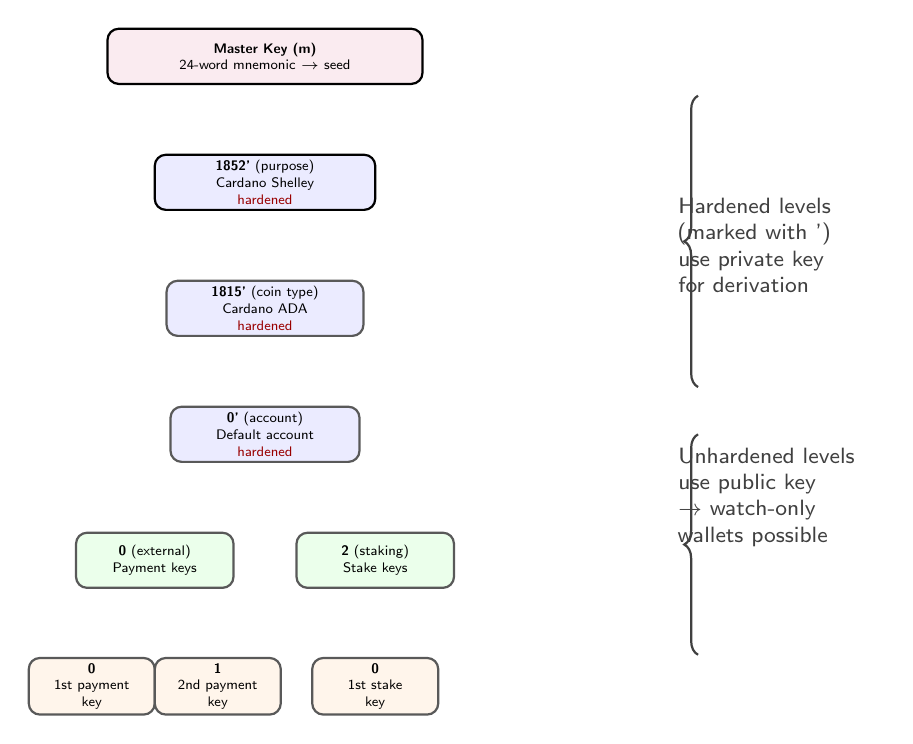
\begin{tikzpicture}[
  level 1/.style={sibling distance=5.5cm, level distance=1.6cm},
  level 2/.style={sibling distance=4cm, level distance=1.6cm},
  level 3/.style={sibling distance=5cm, level distance=1.6cm},
  level 4/.style={sibling distance=2.8cm, level distance=1.6cm},
  level 5/.style={sibling distance=1.6cm, level distance=1.6cm},
  treenode/.style={guidebox, minimum width=1.8cm, minimum height=0.7cm,
    font=\sffamily\tiny, inner sep=2pt},
  edge from parent/.style={guidearrow, thick},
  edge from parent path={(\tikzparentnode.south) -- (\tikzchildnode.north)},
]
  \node[treenode, fill=purple!8, minimum width=4cm]
    {\textbf{Master Key (m)}\\24-word mnemonic $\to$ seed}
    child {
      node[treenode, fill=blue!8, minimum width=2.8cm]
        {\textbf{1852'} (purpose)\\Cardano Shelley\\{\tiny\textcolor{red!60!black}{hardened}}}
      child {
        node[treenode, fill=blue!8, minimum width=2.5cm]
          {\textbf{1815'} (coin type)\\Cardano ADA\\{\tiny\textcolor{red!60!black}{hardened}}}
        child {
          node[treenode, fill=blue!8, minimum width=2.4cm]
            {\textbf{0'} (account)\\Default account\\{\tiny\textcolor{red!60!black}{hardened}}}
          child {
            node[treenode, fill=green!8, minimum width=2cm]
              {\textbf{0} (external)\\Payment keys}
            child {
              node[treenode, fill=orange!8, minimum width=1.6cm]
                {\textbf{0}\\1st payment\\key}
            }
            child {
              node[treenode, fill=orange!8, minimum width=1.6cm]
                {\textbf{1}\\2nd payment\\key}
            }
          }
          child {
            node[treenode, fill=green!8, minimum width=2cm]
              {\textbf{2} (staking)\\Stake keys}
            child {
              node[treenode, fill=orange!8, minimum width=1.6cm]
                {\textbf{0}\\1st stake\\key}
            }
          }
        }
      }
    };

  % Annotations
  \node[guidelabel, text width=2.5cm, align=left] at (6.5,-2.4)
    {Hardened levels\\(marked with ')\\use private key\\for derivation};
  \node[guidelabel, text width=2.5cm, align=left] at (6.5,-5.6)
    {Unhardened levels\\use public key\\$\to$ watch-only\\wallets possible};

  % Bracket for hardened
  \draw[decorate, decoration={brace, amplitude=5pt, mirror},
    thick, gray!50!black]
    (5.5,-0.5) -- (5.5,-4.2) node[midway, right=8pt] {};

  % Bracket for unhardened
  \draw[decorate, decoration={brace, amplitude=5pt, mirror},
    thick, gray!50!black]
    (5.5,-4.8) -- (5.5,-7.6) node[midway, right=8pt] {};
\end{tikzpicture}
\caption{CIP-1852 / BIP-44 hierarchical deterministic wallet derivation tree.
The master key is derived from a 24-word mnemonic.  Purpose (1852'),
coin type (1815'), and account (0') levels use hardened derivation (private
key required), providing a security firewall.  Role and index levels use
unhardened derivation, enabling watch-only wallets.  The credential system
uses \texttt{m/1852'/1815'/0'/0/0} for payment and
\texttt{m/1852'/1815'/0'/2/0} for staking.}
\label{fig:cip1852-derivation}
\end{figure}


% ============================================================================
\section{How the CIPs Work Together}
\label{sec:cips-together}
% ============================================================================

The CIPs described in this chapter are not isolated features---they form an
interlocking system where each standard enables or enhances the others.
Understanding their interactions is essential for understanding the
credential architecture as a whole.

\textbf{CIP-32 enables CIP-68.}  Without inline datums, the Reference
Token's metadata would be stored as a hash, requiring off-chain resolution.
Inline datums make the metadata directly readable on-chain.

\textbf{CIP-31 makes CIP-68 practical.}  Without reference inputs, every
credential verification would consume (and have to recreate) the Reference
Token UTxO, causing contention.  Reference inputs allow unlimited concurrent
reads.

\textbf{CIP-33 makes CIP-68 affordable.}  Without reference scripts, every
transaction interacting with the credential validator would include the full
Plutus script, inflating transaction size and fees.  Reference scripts reduce
per-transaction overhead to a 32-byte pointer.

\textbf{CIP-68 makes CIP-25 revocable.}  CIP-25 provides immutable
attestation (``this credential was issued'').  CIP-68 adds mutable status
(``the credential is currently active/revoked'').  Together, they provide
both historical provenance and current validity.

\textbf{CIP-30 connects users to the system.}  Without the dApp--wallet
bridge, every credential operation would require server-side key management,
creating custodial risk.  CIP-30 keeps private keys under user control.

\textbf{CIP-1852 makes wallets recoverable and interoperable.}  Without
HD derivation, losing a key file means losing all credentials.  With
CIP-1852, 24 words are sufficient to recover everything.

\begin{figure}[ht]
\centering
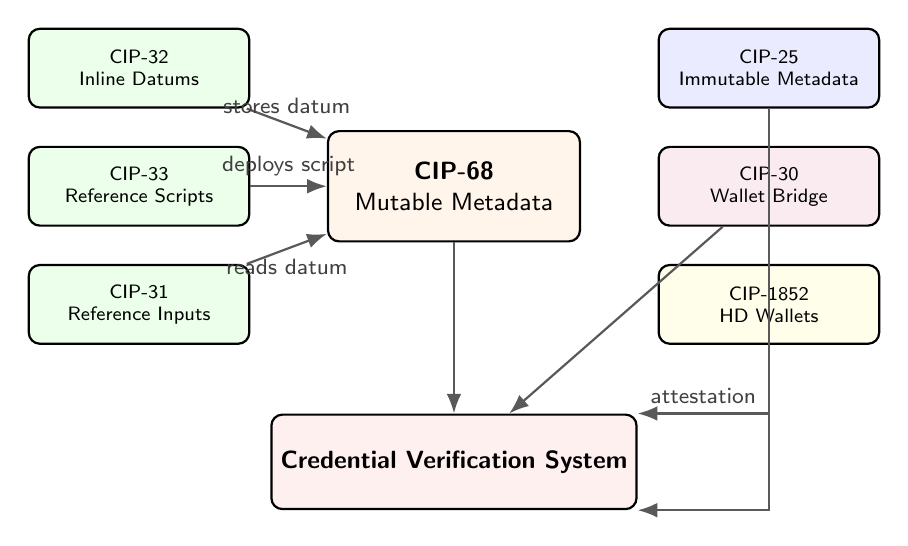
\begin{tikzpicture}[
  cipbox/.style={guidebox, minimum width=2.8cm, minimum height=1cm,
    font=\sffamily\scriptsize},
  node distance=0.6cm and 1.2cm,
]
  % Central: CIP-68
  \node[cipbox, fill=orange!8, minimum width=3.2cm, minimum height=1.4cm,
    font=\sffamily\small] (cip68) at (0,0)
    {\textbf{CIP-68}\\Mutable Metadata};

  % Dependencies feeding into CIP-68
  \node[cipbox, fill=green!8] (cip32) at (-4, 1.5) {CIP-32\\Inline Datums};
  \node[cipbox, fill=green!8] (cip31) at (-4,-1.5) {CIP-31\\Reference Inputs};
  \node[cipbox, fill=green!8] (cip33) at (-4, 0) {CIP-33\\Reference Scripts};

  % CIP-25 companion
  \node[cipbox, fill=blue!8] (cip25) at (4, 1.5) {CIP-25\\Immutable Metadata};

  % CIP-30 and CIP-1852
  \node[cipbox, fill=purple!8] (cip30) at (4, 0) {CIP-30\\Wallet Bridge};
  \node[cipbox, fill=yellow!8] (cip1852) at (4,-1.5) {CIP-1852\\HD Wallets};

  % Credential System
  \node[cipbox, fill=red!6, minimum width=4cm, minimum height=1.2cm,
    font=\sffamily\small] (system) at (0,-3.5)
    {\textbf{Credential Verification System}};

  % Arrows: dependencies
  \draw[guidearrow] (cip32) -- node[above, guidelabel] {stores datum} (cip68);
  \draw[guidearrow] (cip31) -- node[below, guidelabel] {reads datum} (cip68);
  \draw[guidearrow] (cip33) -- node[above, guidelabel] {deploys script} (cip68);

  % Arrows: to system
  \draw[guidearrow] (cip68) -- (system);
  \draw[guidearrow] (cip25) |- node[near end, above, guidelabel] {attestation} (system.north east);
  \draw[guidearrow] (cip30) -- (system);
  \draw[guidearrow] (cip1852) |- (system.south east);
\end{tikzpicture}
\caption{CIP dependency graph for the credential verification system.
CIPs~31, 32, and~33 (the Plutus~V2 trio) form the technical foundation that
makes CIP-68's mutable datum pattern practical and affordable.  CIP-25
provides immutable attestation.  CIP-30 and CIP-1852 handle wallet
connectivity and key management.  All six converge in the credential
verification system.}
\label{fig:cip-dependency}
\end{figure}


% ============================================================================
\section{Chapter Summary}
\label{sec:cips-summary}
% ============================================================================

This chapter examined the eight CIPs that form the technical foundation of
the credential verification system:

\begin{enumerate}[nosep]
  \item \textbf{CIP-25} provides immutable NFT metadata, establishing
    permanent on-chain attestation of credential issuance.
  \item \textbf{CIP-68} introduces the dual-token pattern with mutable
    inline datums, enabling authority-controlled revocation without requiring
    the holder's private key---the key innovation for on-chain credential
    management.
  \item \textbf{CIP-30} defines the non-custodial dApp--wallet bridge,
    keeping private keys under user control while enabling web-based
    credential operations.
  \item \textbf{CIP-31} introduces reference inputs, allowing transactions
    to read UTxO data without consuming it---essential for concurrent
    credential verification.
  \item \textbf{CIP-32} introduces inline datums, storing full data directly
    in UTxOs---the prerequisite for CIP-68's on-chain metadata.
  \item \textbf{CIP-33} introduces reference scripts, reducing transaction
    size and fees by deploying Plutus scripts once and referencing them.
  \item \textbf{CIP-1852} defines HD wallet derivation, providing
    recoverable, interoperable key management from a single mnemonic.
\end{enumerate}

The next chapter will examine how these CIPs are combined in the system
architecture: the smart contract layer, the token taxonomy, and the
transaction workflows that tie everything together.


% ============================================================================
% CHAPTER 4: Smart Contracts on Cardano
% ============================================================================
% ============================================================================
% Chapter 4: Smart Contracts on Cardano
% Part of the Cardano Credential Verification Study Guide
% ============================================================================

\chapter{Smart Contracts on Cardano}
\label{ch:smart-contracts}

% --- TikZ styles for this chapter -------------------------------------------
\tikzset{
  guidebox/.style={draw, rounded corners=4pt, thick, align=center,
    font=\sffamily\small, fill=white, minimum height=1cm},
  guidearrow/.style={-{Latex[length=2.5mm]}, thick, color=gray!70!black},
  guidelabel/.style={font=\sffamily\footnotesize, text=gray!50!black},
}

Smart contracts are the enforcement layer of any blockchain-based system.
They are the reason a credential issued on Cardano is not merely a
database entry with a fancy name---they are what makes the credential
\emph{trustlessly verifiable}. In this chapter we build a complete
mental model of how Cardano smart contracts work, from the simplest
native scripts through full Plutus V2 validators, and then show exactly
how the credential system uses each type. By the end you will understand
why the system can guarantee that \emph{only} a licensed authority can
mint credential tokens, how multiple professionals can sign a work
product concurrently without conflicting, and how license validity can
be automatically linked to periodic dues payments.


% ============================================================================
\section{What is a Smart Contract?}
\label{sec:what-is-smart-contract}
% ============================================================================

\subsection{The Core Idea}

A smart contract is a piece of code that lives on a blockchain and
enforces rules automatically. Think of a vending machine: you insert
the correct amount of money and press a button, and the machine
dispenses the product. No cashier, no negotiation, no trust required.
The rules are mechanical. A smart contract is the digital equivalent---it
encodes rules in software that the blockchain itself enforces, removing
the need for any human intermediary to verify compliance.

In everyday life, a traditional contract says ``Party A agrees to pay
Party B \$100 on January 1st in exchange for Service X.'' Enforcement
depends on good faith, or failing that, a court. A smart contract
encodes the same logic in executable code: when the conditions are met,
the action happens automatically. When the conditions are \emph{not}
met, the action is rejected. There is no appeals process, no
bureaucratic delay, and no possibility of selective enforcement. The
code runs the same way for everyone.

\subsection{Cardano Validators Are Not Ethereum Smart Contracts}

This distinction is critical and trips up nearly everyone coming from
Ethereum. On Ethereum, a smart contract is a long-lived program with
its own persistent storage. You \emph{call functions} on it, it
updates its internal state, and it can call other contracts. It is
like a microservice that lives on the blockchain.

Cardano does not work this way.

On Cardano, a smart contract is a \textbf{validator}---a function that
receives some data and returns \texttt{True} or \texttt{False}. That is
it. The validator does not store state. It does not call other
validators. It does not have methods you invoke. It simply answers one
question: \emph{``Is this transaction allowed to spend this UTxO?''}

The best analogy is a bouncer at a nightclub. The bouncer does not own
the club. The bouncer does not manage the bar inventory. The bouncer
has exactly one job: check IDs at the door and decide ``yes, you may
enter'' or ``no, you may not.'' A Cardano validator is the bouncer for
a UTxO. When someone builds a transaction that tries to spend a UTxO
locked at a script address, the validator examines the transaction and
says ``yes'' or ``no.''

This design has profound consequences. Because validators are stateless
and pure---they examine inputs and produce a boolean---they are
\emph{deterministic}. The same inputs always produce the same output.
You can run the validator locally before submitting the transaction and
know with certainty whether it will succeed. There are no surprises
from concurrent state changes, no front-running attacks that alter the
execution path, and no gas estimation failures from state that changed
between simulation and execution.

\begin{figure}[H]
\centering
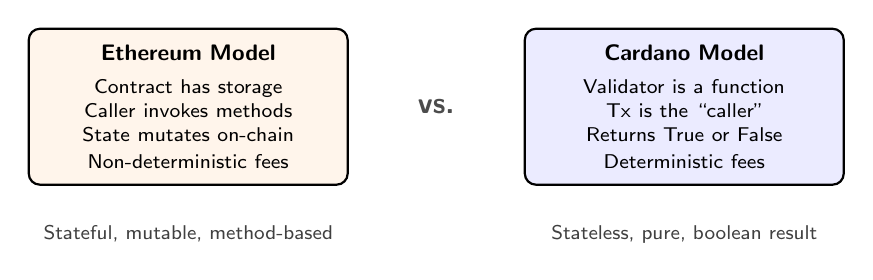
\begin{tikzpicture}[scale=0.9, every node/.style={transform shape}]
  % Ethereum side
  \node[guidebox, fill=orange!8, minimum width=4.5cm, minimum height=2.2cm,
    text width=4cm] (eth) at (-3.5,0) {
    \textbf{Ethereum Model}\\[4pt]
    \footnotesize Contract has storage\\
    \footnotesize Caller invokes methods\\
    \footnotesize State mutates on-chain\\
    \footnotesize Non-deterministic fees
  };
  % Cardano side
  \node[guidebox, fill=blue!8, minimum width=4.5cm, minimum height=2.2cm,
    text width=4cm] (ada) at (3.5,0) {
    \textbf{Cardano Model}\\[4pt]
    \footnotesize Validator is a function\\
    \footnotesize Tx is the ``caller''\\
    \footnotesize Returns True or False\\
    \footnotesize Deterministic fees
  };
  % VS
  \node[font=\sffamily\large\bfseries, text=gray!60!black] at (0,0) {vs.};
  % Labels
  \node[guidelabel] at (-3.5,-1.8) {Stateful, mutable, method-based};
  \node[guidelabel] at (3.5,-1.8) {Stateless, pure, boolean result};
\end{tikzpicture}
\caption{Ethereum's stateful contract model versus Cardano's stateless validator model. Cardano validators are pure functions that approve or reject UTxO spending.}
\label{fig:eth-vs-cardano}
\end{figure}

\subsection{Why This Matters for Credentials}

In the credential system, this design means that the minting policy for
license tokens is a validator that answers: ``Does this transaction
include a signature from the authorized licensing board?'' If yes,
minting proceeds. If no, the transaction is rejected by every node on
the network. There is no admin backdoor, no override function, and no
way to ``call'' the policy and ask it to mint tokens on your behalf.
The only path to minting is constructing a valid transaction that
satisfies the validator's conditions.


% ============================================================================
\section{Native Scripts (Phase 1)}
\label{sec:native-scripts}
% ============================================================================

\subsection{Overview}

Native scripts are Cardano's simplest form of smart contract. They
were introduced in the Shelley era and require no Plutus execution
engine---the ledger evaluates them directly during Phase 1 validation.
This means they incur \textbf{zero execution fees}. The only cost is
the standard transaction fee (${\sim}$0.17~ADA), making them ideal for
operations that need to happen frequently and cheaply.

Native scripts are built from five primitive building blocks. Each
block performs a simple check, and they can be combined to express
sophisticated conditions. Think of them as logic gates: each gate
checks one thing, and you wire them together to build the overall
access policy.

\subsection{The Five Script Types}

\subsubsection{ScriptPubkey: Single Key Requirement}

The simplest native script. It requires that the transaction includes a
signature from a specific verification key hash (public key hash). If
Alice's key hash is embedded in the script, then only a transaction
signed by Alice satisfies the script. This is the script type used for
the credential system's minting policies.

In the credential system, every authority wallet has a unique Ed25519
public key hash (PKH). The minting policy is a \texttt{ScriptPubkey}
containing that PKH. Any transaction that mints or burns tokens under
this policy must be signed by the authority's key. No one else on the
planet can produce a valid signature for that key, so no one else can
create or destroy credential tokens.

\subsubsection{ScriptAll: AND Logic}

Requires that \emph{all} listed conditions are satisfied. If the script
contains three sub-scripts, all three must pass. This is logical AND.

A practical example: a corporate account that requires signatures from
both the CEO and CFO. Neither can act alone. In the credential system,
\texttt{ScriptAll} is used when time-lock constraints are combined with
a key requirement---the authority's key \emph{and} the time constraint
must both be satisfied.

\subsubsection{ScriptAny: OR Logic}

Requires that \emph{at least one} listed condition is satisfied. If the
script contains three sub-scripts, any single one passing is sufficient.
This is logical OR.

A practical example: a recovery mechanism where either the primary key
or a backup key can authorize a transaction. If you lose your primary
key, the backup still works.

\subsubsection{ScriptNofK: Threshold (N-of-K)}

Requires that at least $N$ out of $K$ listed conditions are satisfied.
This generalizes both \texttt{ScriptAll} ($N = K$) and \texttt{ScriptAny}
($N = 1$). A 3-of-5 multi-signature governance scheme uses
\texttt{ScriptNofK} with $N = 3$ and $K = 5$.

This is particularly relevant for the credential system's future
governance upgrade path. Instead of a single authority key controlling
minting, a \texttt{ScriptNofK} policy could require signatures from
3~of~5 board members, distributing trust and eliminating single-key
centralization risk.

\subsubsection{TimeLock: Temporal Constraints}

Two time-lock primitives restrict \emph{when} a script is valid:
\begin{itemize}[nosep]
  \item \textbf{InvalidBefore} (also called \texttt{TimelockStart}):
    the transaction is invalid before a specified slot number. The
    script cannot be satisfied until that slot has passed.
  \item \textbf{InvalidHereAfter} (also called \texttt{TimelockExpiry}):
    the transaction is invalid at or after a specified slot number. The
    script can only be satisfied before that slot.
\end{itemize}

Time locks are used in the credential system to create minting policies
that expire. For example, an authority might create a policy that can
only mint tokens during a specific fiscal year. After the expiry slot,
no new tokens can be minted under that policy, even by the authority.
This provides a cryptographic guarantee that the token supply is frozen
after a certain point.

\begin{figure}[H]
\centering
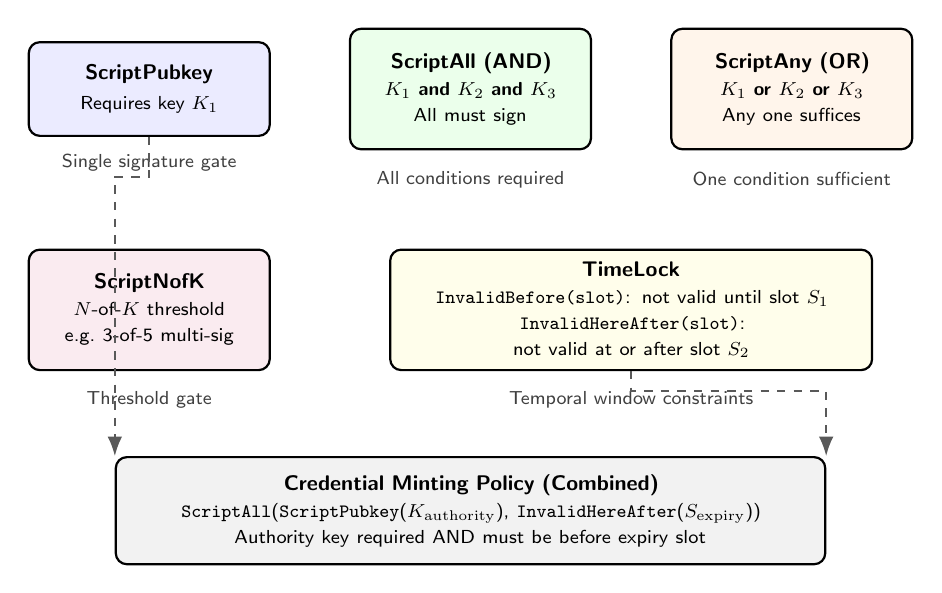
\begin{tikzpicture}[scale=0.85, every node/.style={transform shape}]
  % ScriptPubkey
  \node[guidebox, fill=blue!8, minimum width=3.6cm, minimum height=1.4cm]
    (pk) at (-3.8,4.5)
    {\textbf{ScriptPubkey}\\[2pt]\footnotesize Requires key $K_1$};
  \node[guidelabel] at (-3.8,3.4) {Single signature gate};

  % ScriptAll
  \node[guidebox, fill=green!8, minimum width=3.6cm, minimum height=1.8cm,
    text width=3.2cm] (all) at (1,4.5) {
    \textbf{ScriptAll (AND)}\\[2pt]
    \footnotesize $K_1$ \textbf{and} $K_2$ \textbf{and} $K_3$\\
    \footnotesize All must sign
  };
  \node[guidelabel] at (1,3.15) {All conditions required};

  % ScriptAny
  \node[guidebox, fill=orange!8, minimum width=3.6cm, minimum height=1.8cm,
    text width=3.2cm] (any) at (5.8,4.5) {
    \textbf{ScriptAny (OR)}\\[2pt]
    \footnotesize $K_1$ \textbf{or} $K_2$ \textbf{or} $K_3$\\
    \footnotesize Any one suffices
  };
  \node[guidelabel] at (5.8,3.15) {One condition sufficient};

  % ScriptNofK
  \node[guidebox, fill=purple!8, minimum width=3.6cm, minimum height=1.8cm,
    text width=3.2cm] (nofk) at (-3.8,1.2) {
    \textbf{ScriptNofK}\\[2pt]
    \footnotesize $N$-of-$K$ threshold\\
    \footnotesize e.g.\ 3-of-5 multi-sig
  };
  \node[guidelabel] at (-3.8,-0.15) {Threshold gate};

  % TimeLock
  \node[guidebox, fill=yellow!8, minimum width=7.2cm, minimum height=1.8cm,
    text width=6.8cm] (time) at (3.4,1.2) {
    \textbf{TimeLock}\\[2pt]
    \footnotesize \texttt{InvalidBefore(slot)}: not valid until slot $S_1$\\
    \footnotesize \texttt{InvalidHereAfter(slot)}: not valid at or after slot $S_2$
  };
  \node[guidelabel] at (3.4,-0.15) {Temporal window constraints};

  % Composition example
  \node[guidebox, fill=gray!10, minimum width=10.6cm, minimum height=1.6cm,
    text width=10cm] (combo) at (1,-1.8) {
    \textbf{Credential Minting Policy (Combined)}\\[2pt]
    \footnotesize \texttt{ScriptAll}(\texttt{ScriptPubkey}($K_{\mathrm{authority}}$),
    \texttt{InvalidHereAfter}($S_{\mathrm{expiry}}$))\\
    \footnotesize Authority key required AND must be before expiry slot
  };

  % Arrows to combo
  \draw[guidearrow, dashed] (pk.south) -- ++(0,-0.6) -| (combo.north west);
  \draw[guidearrow, dashed] (time.south) -- ++(0,-0.3) -| (combo.north east);
\end{tikzpicture}
\caption{The five native script types and how they compose. The credential system's minting policy typically combines a \texttt{ScriptPubkey} (authority key) with an optional \texttt{InvalidHereAfter} (time lock) inside a \texttt{ScriptAll} wrapper.}
\label{fig:native-scripts}
\end{figure}

\subsection{Why Native Scripts for Minting Policies?}

The credential system deliberately uses native scripts---not Plutus
validators---for its minting policies. The reason is economics. A
native script minting transaction costs approximately 0.17~ADA with
zero execution fees. A Plutus V2 minting transaction costs 0.3--0.5~ADA
because the Plutus execution engine must evaluate the script, consuming
CPU steps and memory units that are priced into the fee.

For a system that might mint thousands of credential tokens (one license
NFT per professional, plus signature tokens and validity tokens), the
difference compounds. At 10,000 licenses with associated tokens, native
scripts save approximately 1,300--3,300~ADA compared to Plutus-based
minting policies. The trade-off is expressiveness: native scripts can
only check keys and time constraints, while Plutus scripts can examine
the full transaction. For minting policies where the rule is simply
``the authority must sign,'' native scripts provide the same security
guarantee at a fraction of the cost.


% ============================================================================
\section{Plutus V2 Validators (Phase 2)}
\label{sec:plutus-v2}
% ============================================================================

\subsection{Beyond Simple Scripts}

Native scripts answer simple questions: ``Is this key present?'' ``Is
it before slot X?'' But many operations require examining the
\emph{content} of a transaction---which tokens are being moved, what
data is attached, how much ADA is being paid to whom. For these
operations, Cardano provides Plutus validators: full-powered smart
contracts written in Haskell (compiled to Plutus Core, which runs on
the Untyped Plutus Lambda Calculus---UPLC) and evaluated during
Phase~2 validation.

Plutus V2, introduced in the Vasil hard fork (September 2022), added
three features critical for the credential system:
\begin{itemize}[nosep]
  \item \textbf{Reference Inputs (CIP-31)}: read a UTxO without
    consuming it. This lets verifiers inspect credential metadata
    without spending the token.
  \item \textbf{Inline Datums (CIP-32)}: attach data directly to a
    UTxO output instead of storing only a datum hash. This eliminates
    the need to look up datums separately.
  \item \textbf{Reference Scripts (CIP-33)}: reference a script stored
    in a UTxO rather than including the script in every transaction.
    This reduces transaction sizes significantly.
\end{itemize}

\subsection{The Three Inputs to a Validator}

Every Plutus V2 validator receives exactly three pieces of information
when evaluating whether a UTxO can be spent. Understanding these three
inputs is the key to understanding all Cardano smart contracts.

\subsubsection{Datum: The State}

The \textbf{datum} is data attached to the UTxO being spent. Think of
it as a note taped to a locked box. When someone created the UTxO and
sent tokens to the script address, they included this datum to record
the state or context of that particular UTxO.

In the credential system, the \texttt{SignerDatum} is attached to each
signer's deposit UTxO. It records the signer's public key hash, the
SHA-256 hash of the document being signed, the slot at which the
deposit was made, the policy IDs of the signature and validity tokens,
and the validity token's expiry slot. This datum is the ``evidence
packet'' that proves who signed, what they signed, and when.

\subsubsection{Redeemer: The Action}

The \textbf{redeemer} is data provided by the transaction that wants to
spend the UTxO. Think of it as the instruction or request. The datum
says ``here is what was stored.'' The redeemer says ``here is what I
want to do with it.''

In the credential system, the redeemer is an integer discriminator that
tells the validator which action is being performed: \texttt{COLLECT}
(redeemer~0), \texttt{FINALIZE} (redeemer~1), or \texttt{RECLAIM}
(redeemer~2). Each action triggers different validation logic inside the
validator.

\subsubsection{Script Context: The Transaction}

The \textbf{script context} is the full transaction being validated---all
inputs, all outputs, all signatures, all minted tokens, all time
constraints, everything. The validator can inspect any part of the
transaction to make its decision.

This is what gives Plutus validators their power compared to native
scripts. A native script can only check ``is this key present?'' A
Plutus validator can check ``does this transaction include an output
paying exactly 50~ADA to the authority's address?'' or ``does this
transaction mint exactly one token under policy XYZ?''

The validator examines all three inputs---datum, redeemer, and script
context---and returns \texttt{True} (the UTxO may be spent, the
transaction is valid) or \texttt{False} (the spending is rejected, the
transaction fails).

\begin{figure}[H]
\centering
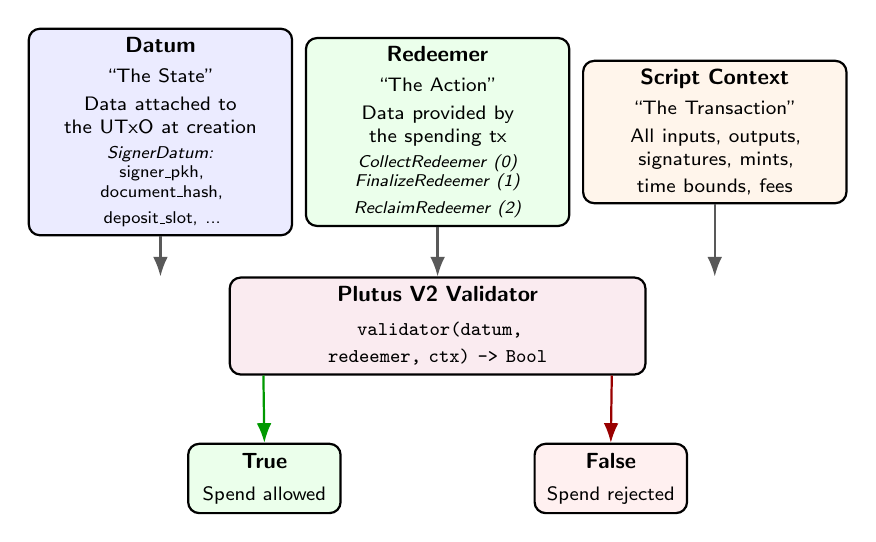
\begin{tikzpicture}[scale=0.88, every node/.style={transform shape}]
  % Datum box
  \node[guidebox, fill=blue!8, minimum width=3.8cm, minimum height=2.0cm,
    text width=3.4cm] (datum) at (-4,2.5) {
    \textbf{Datum}\\[3pt]
    \footnotesize ``The State''\\[2pt]
    \footnotesize Data attached to\\the UTxO at creation\\[2pt]
    \scriptsize\textit{SignerDatum:}\\
    \scriptsize signer\_pkh,\\
    \scriptsize document\_hash,\\
    \scriptsize deposit\_slot, ...
  };

  % Redeemer box
  \node[guidebox, fill=green!8, minimum width=3.8cm, minimum height=2.0cm,
    text width=3.4cm] (redeemer) at (0,2.5) {
    \textbf{Redeemer}\\[3pt]
    \footnotesize ``The Action''\\[2pt]
    \footnotesize Data provided by\\the spending tx\\[2pt]
    \scriptsize\textit{CollectRedeemer (0)}\\
    \scriptsize\textit{FinalizeRedeemer (1)}\\
    \scriptsize\textit{ReclaimRedeemer (2)}
  };

  % ScriptContext box
  \node[guidebox, fill=orange!8, minimum width=3.8cm, minimum height=2.0cm,
    text width=3.4cm] (ctx) at (4,2.5) {
    \textbf{Script Context}\\[3pt]
    \footnotesize ``The Transaction''\\[2pt]
    \footnotesize All inputs, outputs,\\signatures, mints,\\time bounds, fees
  };

  % Validator
  \node[guidebox, fill=purple!8, minimum width=6cm, minimum height=1.4cm,
    text width=5.5cm] (val) at (0,-0.3) {
    \textbf{Plutus V2 Validator}\\[3pt]
    \footnotesize \texttt{validator(datum, redeemer, ctx) -> Bool}
  };

  % Result
  \node[guidebox, fill=green!8, minimum width=2.2cm] (yes) at (-2.5,-2.5) {
    \textbf{True}\\[2pt]\footnotesize Spend allowed
  };
  \node[guidebox, fill=red!6, minimum width=2.2cm] (no) at (2.5,-2.5) {
    \textbf{False}\\[2pt]\footnotesize Spend rejected
  };

  % Arrows in
  \draw[guidearrow] (datum.south) -- (val.north -| datum.south);
  \draw[guidearrow] (redeemer.south) -- (val.north);
  \draw[guidearrow] (ctx.south) -- (val.north -| ctx.south);

  % Arrows out
  \draw[guidearrow, color=green!60!black] (val.south west) ++(0.5,0)
    -- (yes.north);
  \draw[guidearrow, color=red!60!black] (val.south east) ++(-0.5,0)
    -- (no.north);
\end{tikzpicture}
\caption{The three inputs to a Plutus V2 validator. The validator function receives the datum (state stored with the UTxO), the redeemer (action requested by the spending transaction), and the script context (the full transaction), and returns a boolean.}
\label{fig:plutus-validator}
\end{figure}

\subsection{Deterministic Execution}

One of Cardano's most important properties is that Plutus execution is
\textbf{deterministic}. Because the validator is a pure function of its
three inputs, and because the eUTxO model means the inputs are known
before the transaction is submitted, you can run the validator locally
and know \emph{exactly} what will happen on-chain. The fee is
calculable in advance. The result is predictable. There are no
surprises.

This stands in stark contrast to Ethereum, where a transaction can fail
at execution time because another transaction altered the contract's
state between when you simulated it and when it was included in a
block. On Cardano, if the validator succeeds locally, it will succeed
on-chain (assuming the UTxOs have not been spent by another transaction
in the interim---but that is a concurrency issue the eUTxO model makes
explicit, not a hidden state-mutation surprise).


% ============================================================================
\section{Execution Units (exUnits)}
\label{sec:exunits}
% ============================================================================

\subsection{CPU Steps and Memory Units}

Every Plutus script execution consumes two budgeted resources:
\textbf{CPU steps} and \textbf{memory units}. CPU steps measure
computational complexity---how many operations the validator performs.
Memory units measure how much memory the validator allocates during
execution. Both are metered precisely by the UPLC evaluator.

Each transaction has a maximum execution budget, currently set at
10~billion CPU steps and 10~million memory units per transaction (with
per-script limits as well). If a validator exceeds either limit, the
transaction fails. The transaction builder calculates the exact
execution cost before submission, so you know whether you will exceed
the budget before spending any ADA.

\subsection{How exUnits Affect Fees}

Transaction fees on Cardano follow a linear formula:
\[
  \mathrm{fee} = a \times \mathrm{size\_bytes} + b + c_{\mathrm{cpu}} \times \mathrm{cpu\_steps} + c_{\mathrm{mem}} \times \mathrm{mem\_units}
\]
where $a$ and $b$ are the base fee parameters (currently $a = 44$
lovelace per byte, $b = 155{,}381$ lovelace), and $c_{\mathrm{cpu}}$
and $c_{\mathrm{mem}}$ are the execution fee coefficients.

For native scripts, the execution terms ($c_{\mathrm{cpu}}$ and
$c_{\mathrm{mem}}$) are zero---native scripts are evaluated by the
ledger rules themselves, not by the Plutus execution engine. This is
why native script transactions cost ${\sim}$0.17~ADA: only the
size-based fee applies.

For Plutus V2 transactions, the execution terms add 0.1--0.3~ADA
depending on script complexity, bringing the total to ${\sim}$0.3--0.5~ADA.
This is still dramatically cheaper than Ethereum (where gas costs can
reach \$1--\$15+ for contract interactions), but it is a measurable
difference when multiplied across thousands of transactions.

\subsection{Deterministic Cost Estimation}

Because Plutus execution is deterministic, the cost is known
\emph{before} the transaction is submitted to the network. The
transaction builder runs the validator against the exact inputs,
records the CPU and memory consumption, embeds the exUnits in the
transaction, and calculates the precise fee. If the fee changes between
estimation and submission, it is because a UTxO was spent (a
concurrency event), not because the validator behaved differently.

\begin{figure}[H]
\centering
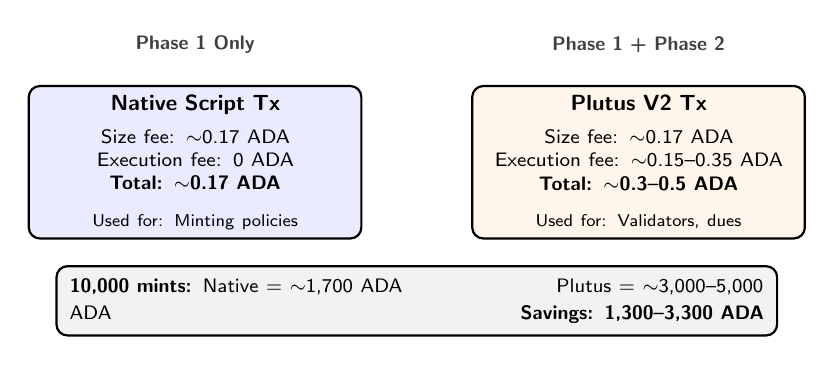
\begin{tikzpicture}[scale=0.88, every node/.style={transform shape}]
  % Native Script
  \node[guidebox, fill=blue!8, minimum width=4.8cm, minimum height=2.2cm,
    text width=4.4cm] (native) at (-3.2,0) {
    \textbf{Native Script Tx}\\[4pt]
    \footnotesize Size fee: ${\sim}$0.17 ADA\\
    \footnotesize Execution fee: 0 ADA\\
    \footnotesize \textbf{Total: ${\sim}$0.17 ADA}\\[4pt]
    \scriptsize Used for: Minting policies
  };

  % Plutus V2
  \node[guidebox, fill=orange!8, minimum width=4.8cm, minimum height=2.2cm,
    text width=4.4cm] (plutus) at (3.2,0) {
    \textbf{Plutus V2 Tx}\\[4pt]
    \footnotesize Size fee: ${\sim}$0.17 ADA\\
    \footnotesize Execution fee: ${\sim}$0.15--0.35 ADA\\
    \footnotesize \textbf{Total: ${\sim}$0.3--0.5 ADA}\\[4pt]
    \scriptsize Used for: Validators, dues
  };

  % Labels
  \node[guidelabel, font=\sffamily\footnotesize\bfseries]
    at (-3.2,1.7) {Phase 1 Only};
  \node[guidelabel, font=\sffamily\footnotesize\bfseries]
    at (3.2,1.7) {Phase 1 + Phase 2};

  % Cost comparison bar
  \node[guidebox, fill=gray!10, minimum width=10.4cm, minimum height=1.0cm,
    text width=10cm] at (0,-2.0) {
    \footnotesize \textbf{10,000 mints:} Native = ${\sim}$1,700 ADA
    \hfill Plutus = ${\sim}$3,000--5,000 ADA
    \hfill \textbf{Savings: 1,300--3,300 ADA}
  };
\end{tikzpicture}
\caption{Fee comparison between native script and Plutus V2 transactions. Native scripts avoid Phase~2 execution costs entirely, making them the economical choice for simple minting policies.}
\label{fig:exunits}
\end{figure}


% ============================================================================
\section{Minting Policies}
\label{sec:minting-policies}
% ============================================================================

\subsection{What is a Minting Policy?}

A minting policy is a special type of validator that controls the
creation (minting) and destruction (burning) of native tokens. On
Cardano, every native token belongs to a \textbf{policy ID}, which is
the Blake2b-224 hash of the minting policy script. The policy ID is
the token's identity---it tells you \emph{which rules govern this
token's existence}.

This is fundamentally different from Ethereum, where token contracts
are long-lived programs that maintain a balance mapping. On Cardano,
tokens are ledger-level assets. The minting policy only runs when
tokens are created or destroyed. Transfers between wallets require no
script execution at all---they are plain UTxO transactions, just like
sending ADA.

\subsection{Policy ID = Script Hash}

The policy ID is computed deterministically:
\[
  \mathrm{PolicyID} = \mathrm{Blake2b}_{224}(\mathrm{CBOR}(\mathrm{script}))
\]
Because the hash is deterministic, anyone can independently verify that
a given policy ID corresponds to a specific script. If the script says
``only Alice's key can mint,'' and you verify the script hash matches
the policy ID, then you know with mathematical certainty that only
Alice can have minted those tokens. No trust required. No authority to
query. Just hash verification.

\subsection{The Credential System's Minting Policy}

In the credential system, the minting policy is a \texttt{ScriptPubkey}
native script containing the authority's public key hash. The
\texttt{PlutusV2MintingPolicy} class (despite its name, it uses native
scripts for economic efficiency) constructs this policy:

\begin{enumerate}[nosep]
  \item The authority's 28-byte Ed25519 verification key hash is
    embedded in a \texttt{ScriptPubkey} native script.
  \item Optionally, time-lock constraints are added via
    \texttt{ScriptAll} (combining the key requirement with
    \texttt{InvalidBefore}/\texttt{InvalidHereAfter}).
  \item The policy ID is the Blake2b-224 hash of the CBOR-serialized
    script.
  \item The policy is saved as both a JSON metadata file and a CBOR
    binary for transaction building.
\end{enumerate}

This means \textbf{only the authority can mint or burn credential
tokens}. A transaction attempting to mint tokens under this policy must
include a valid Ed25519 signature from the authority's private key.
Without that key, no entity---not even Cardano node operators or stake
pool operators---can create tokens under that policy.

\begin{figure}[H]
\centering
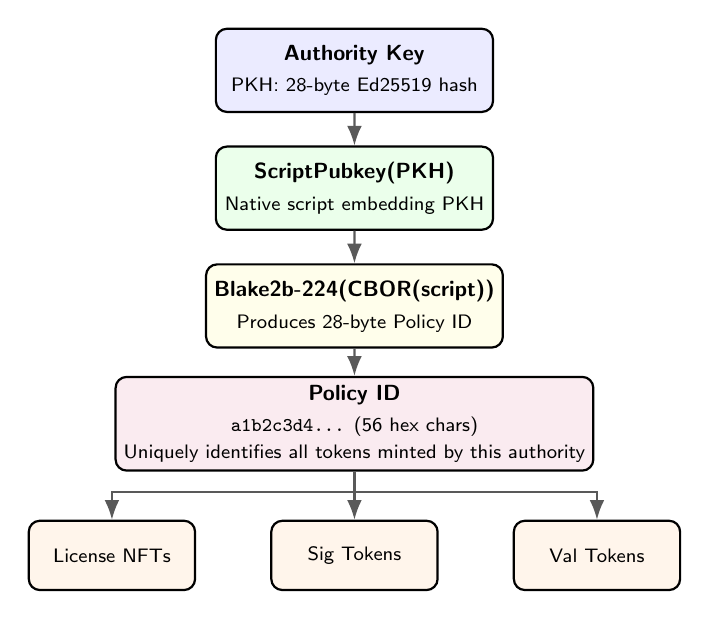
\begin{tikzpicture}[scale=0.88, every node/.style={transform shape}]
  % Authority key
  \node[guidebox, fill=blue!8, minimum width=4cm, minimum height=1.2cm]
    (key) at (0,3.5) {
    \textbf{Authority Key}\\[2pt]
    \footnotesize PKH: 28-byte Ed25519 hash
  };

  % ScriptPubkey
  \node[guidebox, fill=green!8, minimum width=4cm, minimum height=1.2cm]
    (script) at (0,1.8) {
    \textbf{ScriptPubkey(PKH)}\\[2pt]
    \footnotesize Native script embedding PKH
  };

  % CBOR + Hash
  \node[guidebox, fill=yellow!8, minimum width=4cm, minimum height=1.2cm]
    (hash) at (0,0.1) {
    \textbf{Blake2b-224(CBOR(script))}\\[2pt]
    \footnotesize Produces 28-byte Policy ID
  };

  % Policy ID
  \node[guidebox, fill=purple!8, minimum width=6cm, minimum height=1.2cm]
    (pid) at (0,-1.6) {
    \textbf{Policy ID}\\[2pt]
    \footnotesize \texttt{a1b2c3d4...} (56 hex chars)\\
    \footnotesize Uniquely identifies all tokens minted by this authority
  };

  % Tokens
  \node[guidebox, fill=orange!8, minimum width=2.4cm] (t1) at (-3.5,-3.5)
    {\footnotesize License NFTs};
  \node[guidebox, fill=orange!8, minimum width=2.4cm] (t2) at (0,-3.5)
    {\footnotesize Sig Tokens};
  \node[guidebox, fill=orange!8, minimum width=2.4cm] (t3) at (3.5,-3.5)
    {\footnotesize Val Tokens};

  % Arrows
  \draw[guidearrow] (key) -- (script);
  \draw[guidearrow] (script) -- (hash);
  \draw[guidearrow] (hash) -- (pid);
  \draw[guidearrow] (pid.south) -- ++(0,-0.3) -| (t1.north);
  \draw[guidearrow] (pid.south) -- (t2.north);
  \draw[guidearrow] (pid.south) -- ++(0,-0.3) -| (t3.north);
\end{tikzpicture}
\caption{Minting policy derivation: the authority's key hash is embedded in a native script, which is hashed to produce the deterministic Policy ID that governs all credential tokens.}
\label{fig:minting-policy}
\end{figure}

\subsection{Verification Without Trust}

A verifier who wants to confirm that a credential token is legitimate
performs these steps:
\begin{enumerate}[nosep]
  \item Look up the token's policy ID on-chain.
  \item Check that the policy ID is in the registry of known
    authorities (e.g., ``Policy ID \texttt{abc123...} belongs to the
    California Board of Professional Engineers'').
  \item The mathematical relationship between the policy ID and the
    authority's key guarantees that only the authority could have minted
    that token.
\end{enumerate}

No API call to the licensing board. No database query. No waiting for
business hours. The verification is a deterministic mathematical
operation that takes milliseconds.


% ============================================================================
\section{The SignatureCollectionValidator}
\label{sec:signature-collection-validator}
% ============================================================================

\subsection{The Problem: Multi-Party Signing on eUTxO}

The Signature Collection Validator is the most complex and most
important smart contract in the credential system. It solves a problem
that is conceptually simple---collect signatures from multiple
professionals on a single document---but technically challenging on
Cardano's eUTxO model.

The challenge is \textbf{concurrency}. On Ethereum, multiple users can
call the same contract simultaneously because the contract maintains
internal state (a mapping of who has signed). The EVM serializes these
calls and updates the state sequentially. On Cardano's eUTxO model,
there is no shared mutable state. A UTxO can only be spent once. If
two signers try to spend the same UTxO at the same time, one
transaction succeeds and the other fails.

Consider a naive design: a single UTxO at the script address holds the
``work product state'' (which signers have signed so far). Signer~A
builds a transaction that spends this UTxO and creates a new one with
their signature added. Signer~B, working simultaneously, builds a
transaction that also spends the \emph{same original UTxO}. Both
transactions cannot succeed---the first one to be included in a block
wins, and the second fails because the UTxO it references no longer
exists. This is the eUTxO concurrency bottleneck.

\subsection{The Solution: Independent Per-Signer UTxOs}

The credential system's \texttt{SignatureCollectionValidator} solves
this elegantly: instead of maintaining a single shared-state UTxO,
\textbf{each signer creates their own independent UTxO} at the script
address. There is no shared state to contend over. Signer~A deposits
their tokens into one UTxO. Signer~B deposits their tokens into a
different UTxO. Both UTxOs sit at the same script address but are
completely independent. They can be created in the same block, in
different blocks, or even simultaneously---there is zero contention.

Think of it like a suggestion box with individual envelopes. Instead of
everyone writing on the same sheet of paper (which creates a queue),
each person drops their own sealed envelope into the box. The envelopes
do not interfere with each other. When the authority is ready to
finalize, they open all the envelopes at once.

\subsection{The Three Redeemer Actions}

The validator supports three actions, identified by their
\texttt{CONSTR\_ID} discriminator:

\subsubsection{COLLECT (Redeemer 0)}

The \texttt{CollectRedeemer} (constructor ID~0) is used when a signer
deposits their tokens. Any required signer can submit a transaction
that:
\begin{enumerate}[nosep]
  \item Creates a new UTxO at the validator's script address.
  \item Attaches a \texttt{SignerDatum} containing their PKH, the
    document hash, the deposit slot, the policy IDs of their signature
    and validity tokens, and the validity expiry slot.
  \item Includes at least one signature token and one validity token in
    the UTxO's value.
  \item Is signed by the signer's private key (proving ownership of the
    PKH in the datum).
\end{enumerate}

The validator checks that:
\begin{itemize}[nosep]
  \item The signer's PKH is in the list of required signers.
  \item The signer has not already deposited (no duplicate deposits).
  \item The validity token has not expired (expiry slot is in the
    future relative to the current slot).
  \item If a validity deadline is set, the expiry slot does not exceed
    it.
  \item The required tokens (signature token + validity token) are
    present in the UTxO value.
\end{itemize}

This is the critical concurrency-safe operation. Because each
\texttt{COLLECT} creates a \emph{new, independent} UTxO rather than
modifying an existing one, multiple signers can deposit simultaneously
without any risk of transaction collision. Signer~1 in New York and
Signer~2 in Los Angeles can submit their deposit transactions at the
exact same second, and both will succeed because they are creating
different UTxOs, not competing to spend the same one.

\subsubsection{FINALIZE (Redeemer 1)}

The \texttt{FinalizeRedeemer} (constructor ID~1) is used by the
authority to complete the signing process. When all required signers
have deposited their tokens, the authority builds a single transaction
that:
\begin{enumerate}[nosep]
  \item Consumes \emph{all} per-signer UTxOs at the script address as
    inputs (one input per signer).
  \item Creates a single output containing all collected tokens.
  \item Must be signed by the authority's key.
  \item Includes the \texttt{FinalizeRedeemer} for each script input.
\end{enumerate}

This is an \textbf{atomic sweep}: all per-signer deposits are consumed
in a single transaction. Either the finalization succeeds entirely (all
UTxOs are spent and the work product is complete) or it fails entirely
(no UTxOs are spent). There is no partial finalization.

The validator checks that:
\begin{itemize}[nosep]
  \item The transaction is signed by the authority's PKH.
  \item All required signers have deposits present among the inputs.
  \item The document hash in each \texttt{SignerDatum} matches the work
    product's document hash.
\end{itemize}

\subsubsection{RECLAIM (Redeemer 2)}

The \texttt{ReclaimRedeemer} (constructor ID~2) is the escape hatch. If
a work product is cancelled before finalization, signers need a way to
recover their deposited tokens. A signer can submit a reclaim
transaction that:
\begin{enumerate}[nosep]
  \item Consumes their specific UTxO at the script address.
  \item Returns their signature token and validity token to their wallet.
  \item Must be signed by the same key that made the original deposit
    (the signer's PKH in the \texttt{SignerDatum}).
\end{enumerate}

The validator checks that the transaction signer matches the
\texttt{signer\_pkh} in the datum. Only the original depositor can
reclaim their tokens---no one else, not even the authority, can spend a
signer's deposit UTxO via the \texttt{RECLAIM} action.

\subsection{The SignerDatum}

Each deposit UTxO carries a \texttt{SignerDatum}, which is a Plutus
data type (\texttt{PlutusData} subclass with \texttt{CONSTR\_ID = 0})
containing six fields:

\begin{table}[H]
\centering
\small
\begin{tabular}{@{}llp{6.5cm}@{}}
\toprule
\textbf{Field} & \textbf{Type} & \textbf{Description} \\
\midrule
\texttt{signer\_pkh} & \texttt{bytes} & 28-byte public key hash of the signer \\
\texttt{document\_hash} & \texttt{bytes} & SHA-256 hash of the document being signed \\
\texttt{deposit\_slot} & \texttt{int} & Cardano slot number at deposit time \\
\texttt{sig\_token\_policy} & \texttt{bytes} & Policy ID of the signature token \\
\texttt{val\_token\_policy} & \texttt{bytes} & Policy ID of the validity token \\
\texttt{validity\_expiry\_slot} & \texttt{int} & Slot at which the validity token expires \\
\bottomrule
\end{tabular}
\caption{SignerDatum fields. Each deposit UTxO at the validator address carries this datum, creating a complete evidence record for each signer.}
\label{tab:signer-datum}
\end{table}

This datum serves as the on-chain evidence record. After finalization,
anyone can read the datum from the consumed UTxOs (via transaction
history) and independently verify: \emph{who} signed (signer\_pkh),
\emph{what} they signed (document\_hash), \emph{when} they signed
(deposit\_slot), \emph{under what authority} (token policy IDs), and
\emph{whether their credential was valid} at signing time
(validity\_expiry\_slot $>$ deposit\_slot).

\subsection{Concurrency in Detail: The COLLECT $\rightarrow$ FINALIZE Flow}

Let us trace through a concrete example with three signers---Alice
(a structural engineer), Bob (a geotechnical engineer), and Carol
(the project manager)---signing off on a seismic retrofit design.

\begin{figure}[H]
\centering
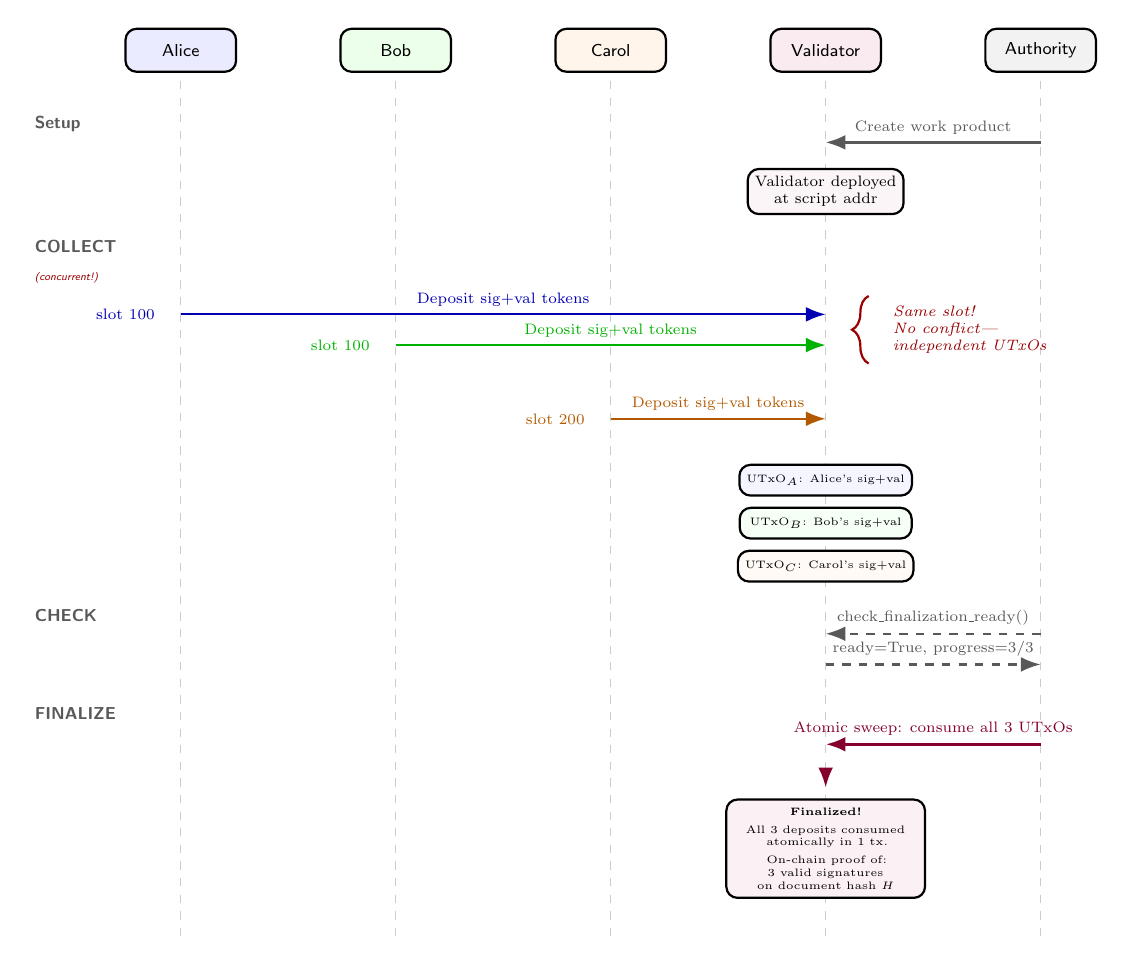
\begin{tikzpicture}[scale=0.78, every node/.style={transform shape}]
  % Actors
  \node[guidebox, fill=blue!8, minimum width=1.8cm, minimum height=0.7cm,
    font=\sffamily\footnotesize] (alice) at (0,0) {Alice};
  \node[guidebox, fill=green!8, minimum width=1.8cm, minimum height=0.7cm,
    font=\sffamily\footnotesize] (bob) at (3.5,0) {Bob};
  \node[guidebox, fill=orange!8, minimum width=1.8cm, minimum height=0.7cm,
    font=\sffamily\footnotesize] (carol) at (7,0) {Carol};
  \node[guidebox, fill=purple!8, minimum width=1.8cm, minimum height=0.7cm,
    font=\sffamily\footnotesize] (val) at (10.5,0) {Validator};
  \node[guidebox, fill=gray!10, minimum width=1.8cm, minimum height=0.7cm,
    font=\sffamily\footnotesize] (auth) at (14,0) {Authority};

  % Lifelines
  \draw[dashed, gray!40] (0,-0.5) -- (0,-14.5);
  \draw[dashed, gray!40] (3.5,-0.5) -- (3.5,-14.5);
  \draw[dashed, gray!40] (7,-0.5) -- (7,-14.5);
  \draw[dashed, gray!40] (10.5,-0.5) -- (10.5,-14.5);
  \draw[dashed, gray!40] (14,-0.5) -- (14,-14.5);

  % Phase 1: Setup
  \node[guidelabel, font=\sffamily\footnotesize\bfseries, text=gray!70!black,
    anchor=west] at (-2.5,-1.2) {Setup};
  \draw[guidearrow] (14,-1.5) -- node[above, font=\scriptsize]
    {Create work product} (10.5,-1.5);
  \node[guidebox, fill=purple!4, minimum width=2.2cm, minimum height=0.6cm,
    font=\scriptsize] at (10.5,-2.3) {Validator deployed\\at script addr};

  % Phase 2: COLLECT (concurrent!)
  \node[guidelabel, font=\sffamily\footnotesize\bfseries, text=gray!70!black,
    anchor=west] at (-2.5,-3.2) {COLLECT};
  \node[guidelabel, font=\sffamily\tiny\itshape, text=red!60!black,
    anchor=west] at (-2.5,-3.7) {(concurrent!)};

  % Alice deposits (slot 100)
  \draw[guidearrow, color=blue!70!black] (0,-4.3) --
    node[above, font=\scriptsize, text=blue!70!black]
    {Deposit sig+val tokens} (10.5,-4.3);
  \node[font=\scriptsize, text=blue!70!black, anchor=east] at (-0.3,-4.3)
    {slot 100};

  % Bob deposits (slot 100 - SAME SLOT!)
  \draw[guidearrow, color=green!70!black] (3.5,-4.8) --
    node[above, font=\scriptsize, text=green!70!black]
    {Deposit sig+val tokens} (10.5,-4.8);
  \node[font=\scriptsize, text=green!70!black, anchor=east] at (3.2,-4.8)
    {slot 100};

  % Highlight: same slot, no conflict!
  \draw[decorate, decoration={brace, amplitude=6pt, mirror},
    thick, red!60!black]
    (11.2,-4.0) -- (11.2,-5.1)
    node[midway, right=8pt, font=\scriptsize\itshape, text=red!60!black,
      text width=2.6cm]
    {Same slot! No conflict---independent UTxOs};

  % Carol deposits (slot 200)
  \draw[guidearrow, color=orange!70!black] (7,-6.0) --
    node[above, font=\scriptsize, text=orange!70!black]
    {Deposit sig+val tokens} (10.5,-6.0);
  \node[font=\scriptsize, text=orange!70!black, anchor=east] at (6.7,-6.0)
    {slot 200};

  % Show UTxOs at validator
  \node[guidebox, fill=blue!4, minimum width=2.8cm, minimum height=0.5cm,
    font=\tiny] at (10.5,-7.0) {UTxO$_A$: Alice's sig+val};
  \node[guidebox, fill=green!4, minimum width=2.8cm, minimum height=0.5cm,
    font=\tiny] at (10.5,-7.7) {UTxO$_B$: Bob's sig+val};
  \node[guidebox, fill=orange!4, minimum width=2.8cm, minimum height=0.5cm,
    font=\tiny] at (10.5,-8.4) {UTxO$_C$: Carol's sig+val};

  % Check readiness
  \node[guidelabel, font=\sffamily\footnotesize\bfseries, text=gray!70!black,
    anchor=west] at (-2.5,-9.2) {CHECK};
  \draw[guidearrow, dashed] (14,-9.5) --
    node[above, font=\scriptsize] {check\_finalization\_ready()} (10.5,-9.5);
  \draw[guidearrow, dashed] (10.5,-10.0) --
    node[above, font=\scriptsize] {ready=True, progress=3/3} (14,-10.0);

  % Phase 3: FINALIZE
  \node[guidelabel, font=\sffamily\footnotesize\bfseries, text=gray!70!black,
    anchor=west] at (-2.5,-10.8) {FINALIZE};
  \draw[guidearrow, color=purple!70!black, line width=1.2pt]
    (14,-11.3) --
    node[above, font=\scriptsize, text=purple!70!black]
    {Atomic sweep: consume all 3 UTxOs} (10.5,-11.3);

  % Show atomic consumption
  \node[guidebox, fill=purple!6, minimum width=3.2cm, minimum height=1.6cm,
    text width=3cm, font=\tiny] at (10.5,-13.0) {
    \textbf{Finalized!}\\[2pt]
    All 3 deposits consumed\\atomically in 1 tx.\\[2pt]
    On-chain proof of:\\3 valid signatures\\on document hash $H$
  };

  \draw[guidearrow, color=purple!70!black]
    (10.5,-11.7) -- (10.5,-12.0);
\end{tikzpicture}
\caption{Sequence diagram showing the COLLECT $\rightarrow$ FINALIZE flow with three signers. Alice and Bob deposit in the same slot without conflict because each creates an independent UTxO. Carol deposits later. The authority then atomically sweeps all three UTxOs in a single finalization transaction.}
\label{fig:collect-finalize}
\end{figure}

\textbf{Step 1: Setup.} The authority creates a
\texttt{SignatureCollectionValidator} parameterized with the three
signers' PKHs, the document hash, and optionally a validity deadline
slot. The validator is deployed (its script hash determines a unique
script address on-chain).

\textbf{Step 2: Alice deposits (slot 100).} Alice builds a transaction
that creates a new UTxO at the validator address containing:
1~signature token, 1~validity token, a \texttt{SignerDatum} with her
PKH and the document hash, and the minimum ADA (${\sim}$2~ADA). The
transaction includes the \texttt{CollectRedeemer}. She signs it with
her private key. The validator approves because her PKH is in
\texttt{required\_signers}, her validity token has not expired, and she
has not already deposited. A new UTxO$_A$ now sits at the script
address.

\textbf{Step 3: Bob deposits (slot 100---same slot!).} Bob does exactly
the same thing at the same time. His transaction creates a \emph{different}
UTxO$_B$ at the same script address. Because UTxO$_A$ and UTxO$_B$ are
separate UTxOs, there is no contention. Both transactions can be
included in the same block. This is the concurrency solution in
action---if this were a shared-state design, one of them would fail.

\textbf{Step 4: Carol deposits (slot 200).} Carol deposits a day later.
She creates UTxO$_C$. The validator now holds three independent UTxOs,
one per signer.

\textbf{Step 5: Authority checks readiness.} The authority calls
\texttt{check\_finalization\_ready()}, which compares
\texttt{\_collected\_signers} against \texttt{required\_signers} and
returns \texttt{ready=True, progress=``3/3''}.

\textbf{Step 6: Authority finalizes.} The authority builds a single
transaction that consumes UTxO$_A$, UTxO$_B$, and UTxO$_C$ as inputs
(each with a \texttt{FinalizeRedeemer}), and creates an output
containing all collected tokens. The authority signs the transaction
with their key. The validator runs once per input, checking that the
authority's signature is present and that all required signers have
deposits. The transaction is submitted atomically---all three UTxOs are
consumed in one block, creating an immutable on-chain record that all
three professionals signed the seismic retrofit design with valid
credentials.

\subsection{What if Something Goes Wrong?}

If the work product is cancelled before all signers have deposited, each
signer who has already deposited can reclaim their tokens using the
\texttt{RECLAIM} redeemer. The validator verifies that the reclaim
transaction is signed by the same key recorded in the
\texttt{SignerDatum}, ensuring that only the original depositor can
recover their tokens. The authority cannot steal deposited tokens, and
neither can other signers.

If a signer's validity token expires between deposit and finalization,
the deposit remains valid---the validator checked validity at deposit
time and recorded the expiry slot in the datum. However, the authority
may choose to reject the finalization and require the signer to renew
their validity token and re-deposit. This policy decision is made
off-chain; the on-chain validator records the facts and lets the
authority act accordingly.


% ============================================================================
\section{The DuesEnforcementContract}
\label{sec:dues-enforcement}
% ============================================================================

\subsection{Linking License Validity to Payments}

Many professional licenses require periodic dues or renewal fees. A
medical license might require annual renewal with continuing education
verification. A PE license might require periodic dues to the state
board. The \texttt{DuesEnforcementContract} automates this link between
payment and validity, ensuring that a professional's license validity
token can only be renewed when dues are paid.

Think of it like a subscription service with a grace period. As long as
you pay, your subscription (validity token) remains active. If you miss
a payment, there is a grace period during which you can still renew by
paying. If the grace period expires, the authority can revoke your
validity entirely, and you must go through a reinstatement process.

\subsection{Contract Parameters}

The contract is parameterized at deployment time with four values:

\begin{table}[H]
\centering
\small
\begin{tabular}{@{}llp{6cm}@{}}
\toprule
\textbf{Parameter} & \textbf{Type} & \textbf{Description} \\
\midrule
\texttt{annual\_dues\_lovelace} & \texttt{int} & Annual dues in lovelace (1~ADA = 1,000,000 lovelace). Must be between 1~ADA and 10,000~ADA. \\
\texttt{grace\_period\_slots} & \texttt{int} & Number of slots after expiry during which renewal is still allowed. Default: 86,400 (${\sim}$1~day). \\
\texttt{license\_ref} & \texttt{int} & Database reference to the license this contract governs. \\
\texttt{authority\_pkh} & \texttt{bytes} & 28-byte PKH of the authority who can revoke. \\
\bottomrule
\end{tabular}
\caption{DuesEnforcementContract parameters.}
\label{tab:dues-params}
\end{table}

\subsection{Two Redeemer Actions}

\subsubsection{PayDues (Redeemer 0)}

The \texttt{PayDuesRedeemer} (constructor ID~0) is used when a licensee
pays their annual dues. The validator checks:
\begin{itemize}[nosep]
  \item The payment amount is at least \texttt{annual\_dues\_lovelace}.
    Overpayment is allowed; underpayment is rejected.
  \item The payment is directed to the authority's address.
  \item If the current validity has expired, the current slot must be
    within the grace period (current slot $\leq$ expiry slot $+$
    grace period).
\end{itemize}

Upon successful validation, the off-chain system mints a new validity
token with an updated expiry slot (current slot + one year's worth of
slots) and delivers it to the licensee's wallet.

\subsubsection{RevokeValidity (Redeemer 1)}

The \texttt{RevokeValidityRedeemer} (constructor ID~1) is used by the
authority to revoke a license's validity when dues remain unpaid past
the grace period. The validator checks that the transaction is signed
by the authority's key. Upon successful revocation, the licensee can no
longer sign documents---the \texttt{check\_validity\_for\_signing()}
function will return \texttt{False} for any expired validity token,
and even the grace period does not extend signing rights (it only
extends the \emph{renewal} window).

\subsection{Grace Period Mechanics}

The grace period is a carefully designed buffer between ``your validity
expired'' and ``your license is revoked.'' During the grace period:

\begin{itemize}[nosep]
  \item \textbf{Signing is blocked.} An expired validity token prevents
    document signing, even during the grace period. This protects the
    public---an engineer with expired credentials should not be
    stamping designs.
  \item \textbf{Renewal is allowed.} The licensee can pay dues and
    receive a new validity token. This prevents harsh penalties for
    minor payment delays.
  \item \textbf{Revocation is deferred.} The authority cannot revoke
    until the grace period has passed, giving the licensee fair notice
    and opportunity to cure.
\end{itemize}

After the grace period expires without payment, the authority can submit
a revocation transaction. At that point, the licensee must go through a
full reinstatement process (which may involve re-application, additional
fees, and board review).

\begin{figure}[H]
\centering
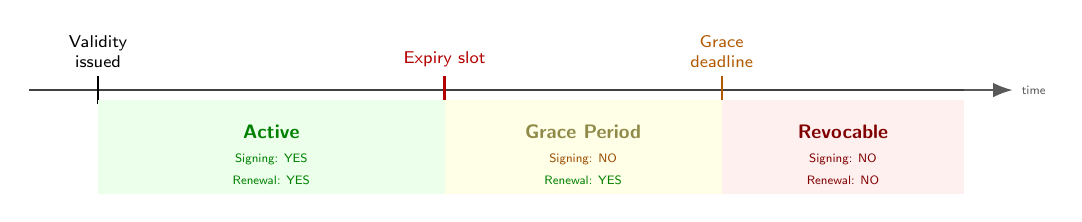
\begin{tikzpicture}[scale=0.88, every node/.style={transform shape}]
  % Timeline
  \draw[thick, gray!50!black] (-1,0) -- (13,0);
  \draw[thick] (0,-0.2) -- (0,0.2) node[above, font=\sffamily\scriptsize, text width=1.5cm, align=center]
    {Validity issued};
  \draw[thick, red!70!black] (5,-0.2) -- (5,0.2)
    node[above, font=\sffamily\scriptsize, text=red!70!black, text width=1.5cm, align=center]
    {Expiry slot};
  \draw[thick, orange!70!black] (9,-0.2) -- (9,0.2)
    node[above, font=\sffamily\scriptsize, text=orange!70!black, text width=1.5cm, align=center]
    {Grace deadline};

  % Zones
  \fill[green!8] (0,-0.15) rectangle (5,-1.5);
  \fill[yellow!10] (5,-0.15) rectangle (9,-1.5);
  \fill[red!6] (9,-0.15) rectangle (12.5,-1.5);

  % Zone labels
  \node[font=\sffamily\footnotesize, text=green!50!black]
    at (2.5,-0.6) {\textbf{Active}};
  \node[font=\sffamily\tiny, text=green!50!black]
    at (2.5,-1.0) {Signing: YES};
  \node[font=\sffamily\tiny, text=green!50!black]
    at (2.5,-1.3) {Renewal: YES};

  \node[font=\sffamily\footnotesize, text=yellow!50!black]
    at (7,-0.6) {\textbf{Grace Period}};
  \node[font=\sffamily\tiny, text=orange!60!black]
    at (7,-1.0) {Signing: NO};
  \node[font=\sffamily\tiny, text=green!50!black]
    at (7,-1.3) {Renewal: YES};

  \node[font=\sffamily\footnotesize, text=red!50!black]
    at (10.75,-0.6) {\textbf{Revocable}};
  \node[font=\sffamily\tiny, text=red!50!black]
    at (10.75,-1.0) {Signing: NO};
  \node[font=\sffamily\tiny, text=red!50!black]
    at (10.75,-1.3) {Renewal: NO};

  % Time arrow
  \draw[guidearrow] (12.5,0) -- (13.2,0)
    node[right, font=\sffamily\tiny] {time};
\end{tikzpicture}
\caption{Dues enforcement timeline. The active period allows both signing and renewal. The grace period blocks signing but allows dues payment. After the grace deadline, the authority can revoke.}
\label{fig:dues-timeline}
\end{figure}

\subsection{The DuesContractDatum}

The on-chain datum for the dues contract is a \texttt{PlutusData}
subclass with \texttt{CONSTR\_ID = 0}, containing four fields:
\texttt{authority\_pkh} (bytes), \texttt{annual\_dues} (int),
\texttt{license\_ref} (int), and \texttt{grace\_period\_slots} (int).
This datum is attached to the contract's UTxO and can be read by any
verifier to understand the dues terms for a given license.

The contract's native script is a \texttt{ScriptPubkey} requiring the
authority's key, ensuring that only the authority can deploy and manage
dues enforcement terms. The contract address is derived from the script
hash, just as with the signature collection validator.


% ============================================================================
\section{Aiken: The Future}
\label{sec:aiken}
% ============================================================================

\subsection{The Problem with PlutusTx}

PlutusTx, the current standard for writing Plutus validators, compiles
Haskell code to Plutus Core (UPLC). While Haskell is a powerful
language well-suited to formal verification, it has practical drawbacks
for smart contract development:

\begin{itemize}[nosep]
  \item \textbf{Large compiled output.} PlutusTx scripts compile to
    relatively large UPLC bytecode. Larger scripts mean larger
    transactions, higher fees, and a tighter budget against the 16~KB
    maximum transaction size.
  \item \textbf{High exUnits.} The compiled UPLC tends to be verbose,
    consuming more CPU steps and memory units than hand-optimized code.
  \item \textbf{Steep learning curve.} Haskell is notoriously difficult
    for developers accustomed to Python, JavaScript, or Rust. This
    limits the pool of potential contributors and auditors.
  \item \textbf{Complex toolchain.} Setting up a PlutusTx development
    environment requires GHC, Cabal, and numerous Haskell dependencies
    that can be challenging to configure.
\end{itemize}

\subsection{Enter Aiken}

Aiken is a modern smart contract language designed specifically for
Cardano. It compiles directly to UPLC without going through Haskell,
producing smaller, more efficient bytecode. Key advantages:

\begin{itemize}[nosep]
  \item \textbf{Smaller compiled scripts.} Aiken-compiled validators
    are typically 40--60\% smaller than equivalent PlutusTx output.
    Smaller scripts mean lower fees and more headroom within the 16~KB
    transaction limit.
  \item \textbf{Lower exUnits.} The tighter UPLC output consumes fewer
    CPU steps and memory units, directly reducing execution fees.
  \item \textbf{Rust-like syntax.} Aiken's syntax is inspired by Rust
    and Gleam, making it accessible to a much broader developer
    community than Haskell.
  \item \textbf{Fast compilation.} Aiken compiles in seconds, compared
    to minutes for a full PlutusTx build. This dramatically improves
    the development feedback loop.
  \item \textbf{Built-in testing.} Aiken includes a native test
    framework with property-based testing support, making it easier to
    write comprehensive validator tests.
\end{itemize}

\subsection{Migration Roadmap (v4.0)}

The credential system's v4.0 roadmap includes migrating the
\texttt{SignatureCollectionValidator} and \texttt{DuesEnforcementContract}
from their current PyCardano-based Plutus V2 implementation to
Aiken-compiled validators. The expected benefits are:

\begin{enumerate}[nosep]
  \item \textbf{Fee reduction:} 20--40\% lower execution fees due to
    smaller, more efficient UPLC bytecode.
  \item \textbf{Audit accessibility:} Aiken's readable syntax makes
    third-party security audits more practical and less expensive.
  \item \textbf{Plutus V3 features:} Aiken supports Plutus V3 natively,
    enabling the use of new built-in functions and cryptographic
    primitives (including BLS12-381 for future zero-knowledge proof
    integration).
  \item \textbf{Community contribution:} A lower barrier to entry means
    more developers can review, test, and contribute to the validator
    logic.
\end{enumerate}

The migration does not change the system's architecture or token model.
The same \texttt{SignerDatum} structure, the same three-redeemer
validator pattern, and the same native-script minting policies will be
preserved. Only the validator implementation language changes---from
Haskell/PlutusTx to Aiken---producing the same logical behavior with
better performance characteristics.

\begin{figure}[H]
\centering
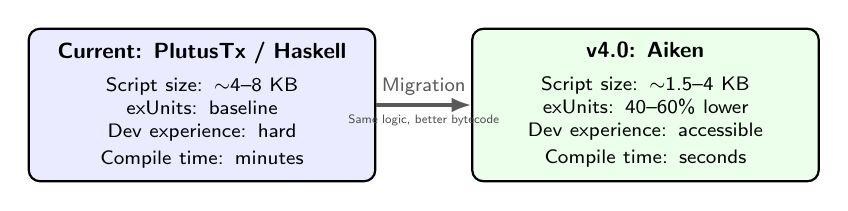
\begin{tikzpicture}[scale=0.88, every node/.style={transform shape}]
  % Current
  \node[guidebox, fill=blue!8, minimum width=5cm, minimum height=2.2cm,
    text width=4.5cm] (current) at (-3.2,0) {
    \textbf{Current: PlutusTx / Haskell}\\[4pt]
    \footnotesize Script size: ${\sim}$4--8 KB\\
    \footnotesize exUnits: baseline\\
    \footnotesize Dev experience: hard\\
    \footnotesize Compile time: minutes
  };

  % Future
  \node[guidebox, fill=green!8, minimum width=5cm, minimum height=2.2cm,
    text width=4.5cm] (future) at (3.2,0) {
    \textbf{v4.0: Aiken}\\[4pt]
    \footnotesize Script size: ${\sim}$1.5--4 KB\\
    \footnotesize exUnits: 40--60\% lower\\
    \footnotesize Dev experience: accessible\\
    \footnotesize Compile time: seconds
  };

  % Arrow
  \draw[guidearrow, line width=1.2pt] (current.east) --
    node[above, font=\sffamily\footnotesize] {Migration}
    node[below, font=\sffamily\tiny, text=gray!60!black]
    {Same logic, better bytecode} (future.west);
\end{tikzpicture}
\caption{Planned migration from PlutusTx/Haskell to Aiken. The validator logic and system architecture remain identical; only the implementation language changes, yielding smaller scripts and lower fees.}
\label{fig:aiken-migration}
\end{figure}

\vspace{1em}
\begin{center}
\rule{0.6\textwidth}{0.4pt}
\end{center}
\vspace{0.5em}

\noindent\textbf{Chapter Summary.} Cardano smart contracts are
validators---pure functions that return \texttt{True} or \texttt{False}
when a transaction attempts to spend a UTxO. Native scripts provide
simple, zero-fee key and time checks ideal for minting policies. Plutus
V2 validators provide full transaction inspection for complex logic like
signature collection and dues enforcement. The credential system uses
native scripts for minting (keeping costs at ${\sim}$0.17~ADA) and
Plutus V2 validators for multi-party signing and payment enforcement
(${\sim}$0.3--0.5~ADA). The \texttt{SignatureCollectionValidator}
solves eUTxO concurrency through independent per-signer UTxOs, and the
\texttt{DuesEnforcementContract} links license validity to periodic
payments with a configurable grace period. Future migration to Aiken
will reduce script sizes and fees while preserving identical logic.


% ============================================================================
% CHAPTER 5: The Credential Verification System
% ============================================================================
% ============================================================================
% Chapter 5: The Credential Verification System
% Study Guide — Blockchain-Based Professional Credential Verification
% ============================================================================

\chapter{The Credential Verification System}
\label{ch:credential-system}

\begin{quote}
\textit{``The preceding chapters established what a blockchain is, how Cardano works, what eUTxO means, and how native tokens and smart contracts operate. This chapter puts all of those pieces together into a single, working application: a credential verification system built on Cardano.''}
\end{quote}

\bigskip

This chapter describes the actual system---every layer, every token, every role, every lifecycle step, and every cost. By the end, you should be able to trace a professional license from its creation on-chain through signing, renewal, revocation, and third-party verification, and explain exactly why each architectural decision was made.

% ============================================================================
\section{System Overview}
\label{sec:ch5-overview}

The credential verification system is organized into three distinct layers, each with a clearly defined responsibility. No single layer can operate in isolation; together they form a complete pipeline from user interaction to immutable on-chain settlement. Understanding this layered separation is essential because it explains why certain operations are fast (local database queries), why others are slow but final (blockchain transactions), and why the middle layer exists at all (to bridge the gap between the two).

\subsection{Layer 1: Cardano Blockchain}

The bottom layer is the Cardano blockchain itself. It provides three critical services that no other layer can replicate: \textbf{token custody} (who holds which tokens is determined by the UTxO set on-chain, not by any off-chain record), \textbf{policy enforcement} (minting policies are evaluated by every node in the network---no single party can bypass them), and \textbf{transaction finality} (once a transaction is confirmed in a block and buried under subsequent blocks, it is irreversible for all practical purposes). The blockchain does not store personal information, does not render dashboards, and does not manage workflow state. It is a settlement layer: slow, expensive relative to a database query, but absolutely authoritative.

Every credential in the system ultimately exists as a Cardano native token. A license is an NFT under a specific minting policy. Signature capacity is a fungible token under the same policy. Validity is a time-bounded token. The blockchain knows nothing about ``licenses'' or ``signatures'' in a semantic sense---it knows only that certain tokens exist at certain addresses under certain policies, and that those policies were satisfied at minting time. All semantic meaning is encoded in metadata and interpreted by the layers above.

\subsection{Layer 2: Off-Chain Application Layer}

The middle layer is a Python application (built on PyCardano v0.19.1) that handles everything the blockchain cannot do efficiently: \textbf{wallet management} (generating HD wallets from mnemonics, deriving keys, encrypting private keys at rest), \textbf{metadata validation} (ensuring CIP-68 metadata conforms to the expected schema before a transaction is built), and \textbf{workflow orchestration} (coordinating multi-step processes like ``mint a license, then mint signature tokens, then mint a validity token, then transfer all three to the licensee''). This layer speaks to the blockchain exclusively through the Blockfrost API, an indexed read/write interface that eliminates the need to run a full Cardano node.

The application layer is where business logic lives. It knows what a ``license'' means, what fields a ``credential'' should have, which wallets are ``authorities'' versus ``licensees,'' and what sequence of transactions constitutes a ``signing ceremony.'' It translates human intent into Cardano transactions and translates on-chain state back into human-readable status.

\subsection{Layer 3: Local SQLite Database}

The top layer is a local SQLite database with nine tables that cache and extend the on-chain state. It exists for three reasons: \textbf{state tracking} (the blockchain is append-only and has no concept of ``current status''---the database maintains derived state like ``this license is active'' by interpreting the chain of transactions), \textbf{caching} (querying the blockchain for every dashboard refresh would be slow and rate-limited; the database provides sub-5ms responses for common queries), and \textbf{dashboard queries} (the web dashboard and CLI tools query the database, not the blockchain, for all read operations). The database is never the source of truth for token ownership---that is always the blockchain. If the database and the chain disagree, the chain wins, and periodic reconciliation corrects the database.

\subsection{Communication: The Blockfrost API}

All communication between the application layer and the Cardano blockchain flows through Blockfrost, a hosted API service that indexes the entire Cardano ledger and exposes it through RESTful endpoints. Blockfrost provides UTxO queries (``what tokens does this address hold?''), transaction submission (``submit this signed transaction to the network''), and chain tip queries (``what is the current slot number?''). The system does not run a full Cardano node. This is a deliberate trade-off: reduced infrastructure cost and complexity in exchange for a dependency on an external service. The risk is mitigated by the existence of multiple Blockfrost alternatives (Koios, Ogmios, self-hosted Blockfrost) and the fact that Blockfrost is a read/write \emph{interface} to the chain, not the chain itself---switching providers does not affect any on-chain state.

\begin{figure}[htbp]
\centering
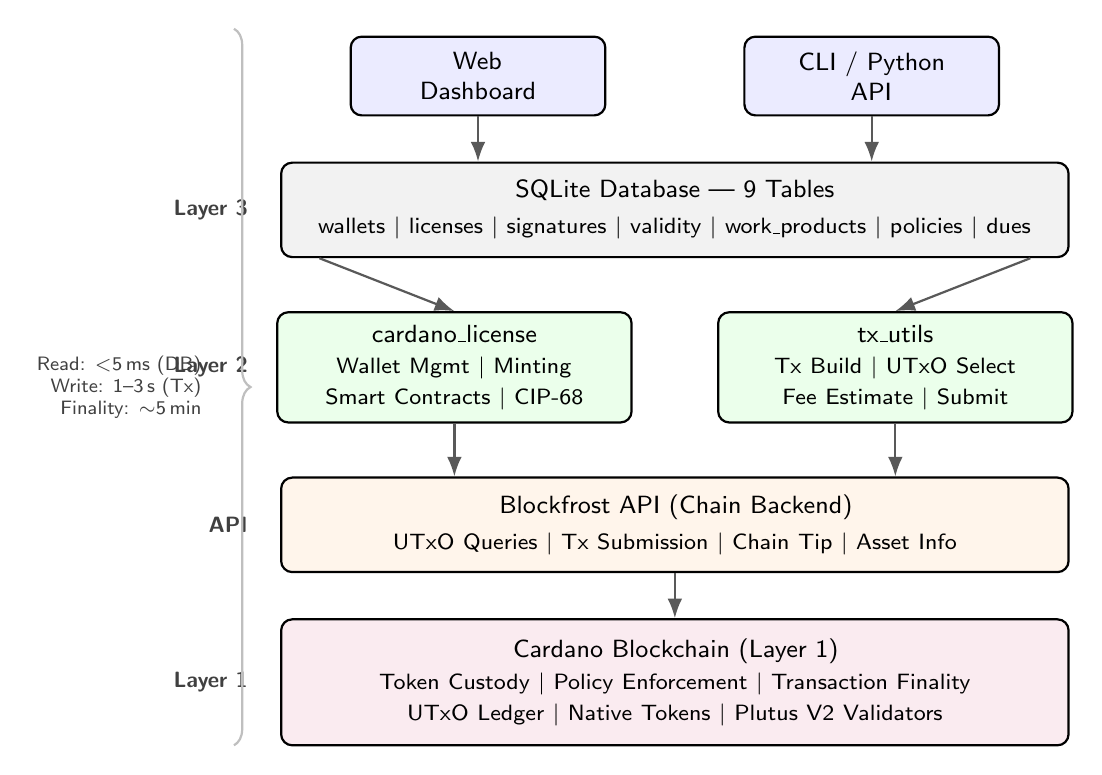
\begin{tikzpicture}[
  guidebox/.style={draw, rounded corners=4pt, thick, align=center, font=\sffamily\small, fill=white, minimum height=1cm},
  guidearrow/.style={-{Latex[length=2.5mm]}, thick, color=gray!70!black},
  guidelabel/.style={font=\sffamily\footnotesize, text=gray!50!black},
]
  % --- Layer 3: Local Database ---
  \node[guidebox, fill=blue!8, minimum width=3.2cm, text width=3cm] (dash) at (-2.5, 8.5) {Web\\Dashboard};
  \node[guidebox, fill=blue!8, minimum width=3.2cm, text width=3cm] (cli) at (2.5, 8.5) {CLI / Python\\API};

  \node[guidebox, fill=gray!10, minimum width=10cm, minimum height=1.2cm, text width=9.5cm] (db) at (0, 6.8)
    {SQLite Database --- 9 Tables\\[2pt]
    \footnotesize wallets $|$ licenses $|$ signatures $|$ validity $|$ work\_products $|$ policies $|$ dues};
  \node[guidelabel, anchor=east] at (-5.3, 6.8) {\textbf{Layer 3}};

  % --- Layer 2: Application ---
  \node[guidebox, fill=green!8, minimum width=4.5cm, minimum height=1.4cm, text width=4cm] (app1) at (-2.8, 4.8)
    {cardano\_license\\[2pt]\footnotesize Wallet Mgmt $|$ Minting\\Smart Contracts $|$ CIP-68};
  \node[guidebox, fill=green!8, minimum width=4.5cm, minimum height=1.4cm, text width=4cm] (app2) at (2.8, 4.8)
    {tx\_utils\\[2pt]\footnotesize Tx Build $|$ UTxO Select\\Fee Estimate $|$ Submit};
  \node[guidelabel, anchor=east] at (-5.3, 4.8) {\textbf{Layer 2}};

  % --- Blockfrost ---
  \node[guidebox, fill=orange!8, minimum width=10cm, minimum height=1.2cm, text width=9.5cm] (bf) at (0, 2.8)
    {Blockfrost API (Chain Backend)\\[2pt]
    \footnotesize UTxO Queries $|$ Tx Submission $|$ Chain Tip $|$ Asset Info};
  \node[guidelabel, anchor=east] at (-5.3, 2.8) {\textbf{API}};

  % --- Layer 1: Blockchain ---
  \node[guidebox, fill=purple!8, minimum width=10cm, minimum height=1.6cm, text width=9.5cm] (chain) at (0, 0.8)
    {Cardano Blockchain (Layer 1)\\[2pt]
    \footnotesize Token Custody $|$ Policy Enforcement $|$ Transaction Finality\\
    \footnotesize UTxO Ledger $|$ Native Tokens $|$ Plutus V2 Validators};
  \node[guidelabel, anchor=east] at (-5.3, 0.8) {\textbf{Layer 1}};

  % --- Arrows ---
  \draw[guidearrow] (dash.south) -- (db.north -| dash);
  \draw[guidearrow] (cli.south) -- (db.north -| cli);
  \draw[guidearrow] (db.south west) ++(0.5,0) -- (app1.north);
  \draw[guidearrow] (db.south east) ++(-0.5,0) -- (app2.north);
  \draw[guidearrow] (app1.south) -- (bf.north -| app1);
  \draw[guidearrow] (app2.south) -- (bf.north -| app2);
  \draw[guidearrow] (bf.south) -- (chain.north);

  % --- Side annotations ---
  \draw[decorate, decoration={brace, amplitude=6pt, mirror}, thick, gray!50]
    (-5.6, 0) -- (-5.6, 9.1) node[midway, left=8pt, align=right, font=\sffamily\scriptsize, text=gray!50!black]
    {Read: $<$5\,ms (DB)\\Write: 1--3\,s (Tx)\\Finality: $\sim$5\,min};

\end{tikzpicture}
\caption{Three-layer architecture of the credential verification system. Layer~1 (Cardano blockchain) provides settlement finality. Layer~2 (off-chain application) handles business logic and transaction construction. Layer~3 (SQLite) provides fast reads and state caching. All chain communication flows through the Blockfrost API.}
\label{fig:ch5-architecture}
\end{figure}


% ============================================================================
\section{Token Taxonomy}
\label{sec:ch5-tokens}

The system defines four distinct token types, all minted under authority-controlled native script policies. Each token serves a specific purpose in the credential lifecycle, and understanding what each token represents---and who holds it---is fundamental to understanding how the system works. These are not abstract concepts; each token is a real Cardano native asset that occupies a UTxO on-chain, carries a minimum ADA deposit, and can be independently verified by anyone with access to the blockchain.

\subsection{Token 1: License NFT (CIP-68)}

The License NFT is the core credential token. It is \textbf{non-fungible}---each one is unique, representing a specific license held by a specific individual. Unlike simple CIP-25 NFTs (which store metadata in the minting transaction's auxiliary data and are immutable thereafter), the License NFT uses the \textbf{CIP-68 datum metadata standard}, which splits the token into a dual-token pair:

\begin{itemize}[nosep]
  \item \textbf{User Token (label 222):} Held in the licensee's personal wallet. This token is \emph{immutable}---its asset name is fixed at minting time and cannot be changed. It serves as a ``badge'' that the licensee can present to prove they were issued a credential. However, the User Token alone does not prove the credential is \emph{currently valid}---it only proves it was once issued.
  \item \textbf{Reference Token (label 100):} Held at the authority's UTxO (or at a known script address). This token carries an \textbf{inline datum} containing the credential's mutable metadata: license type, jurisdiction, issue date, licensee identity, and---critically---a \texttt{status} field. Because the authority controls the UTxO holding the Reference Token, the authority can update the datum at any time (by spending the UTxO and creating a new one with updated datum) without requiring the licensee's cooperation.
\end{itemize}

The CIP-68 pattern is the architectural foundation of the entire revocation mechanism (detailed in Section~\ref{sec:ch5-revocation}). The key insight is that verification always checks the Reference Token's datum, not the User Token. The User Token in the licensee's wallet is a pointer; the Reference Token at the authority's address is the source of truth.

\subsection{Token 2: Signature Token (Fungible)}

Signature tokens represent \textbf{signing capacity}. They are fungible---one signature token is identical to another under the same policy. When the authority issues a license, it also mints a quantity \texttt{N} of signature tokens and transfers them to the licensee's wallet. Each time the licensee signs a document (or, more precisely, participates in a signing ceremony), one signature token is consumed: it is \textbf{deposited into a validator script address} as part of a transaction. The token is not burned; it is locked at the validator, creating a permanent on-chain record that the signing event occurred.

The quantity \texttt{N} determines how many documents the licensee can sign before needing additional tokens. This creates a natural metering mechanism: a professional engineering board might issue 100 signature tokens per year, corresponding to the expected number of documents a PE would stamp. Running out of signature tokens requires requesting more from the authority, which can impose whatever verification it deems appropriate before minting additional tokens.

\subsection{Token 3: Validity Token (Time-Bounded)}

The validity token represents \textbf{current good standing}. It is a native token with a \textbf{slot-based expiry} encoded in its datum or asset name. The validator script that accepts signature deposits also requires a validity token to accompany each deposit. The validator checks that the validity token's expiry slot is in the future at the time of the transaction. If the validity token has expired, the transaction fails---the licensee cannot sign documents until they obtain a new validity token.

Validity tokens are linked to the dues enforcement contract. When a licensee pays their annual dues (or satisfies whatever renewal criteria the authority requires), the authority mints a new validity token with an expiry slot set to the appropriate future date. This creates a direct, enforceable link between license renewal and signing capacity: if you do not renew, your validity token expires, and you cannot deposit signatures into any validator.

\subsection{Token 4: Work Product (Logical Composite)}

A work product is not a single token but a \textbf{logical composite} tracked in the local SQLite database and coordinated by the \texttt{SignatureCollectionValidator} script. A work product represents a document or project that requires signatures from multiple parties---for example, a set of engineering drawings that need stamps from both the designing engineer and the reviewing engineer.

The validator script address accumulates deposits: each required signer creates a separate UTxO at the script address containing their signature token, their validity token, and a datum identifying the work product (by document hash). When all required signers have deposited, the authority submits a \texttt{Finalize} transaction that consumes all deposit UTxOs atomically. The finalized work product is recorded on-chain as a set of consumed UTxOs under the validator script, with each UTxO containing the signer's public key hash, the document hash, and the deposit slot.

\begin{figure}[htbp]
\centering
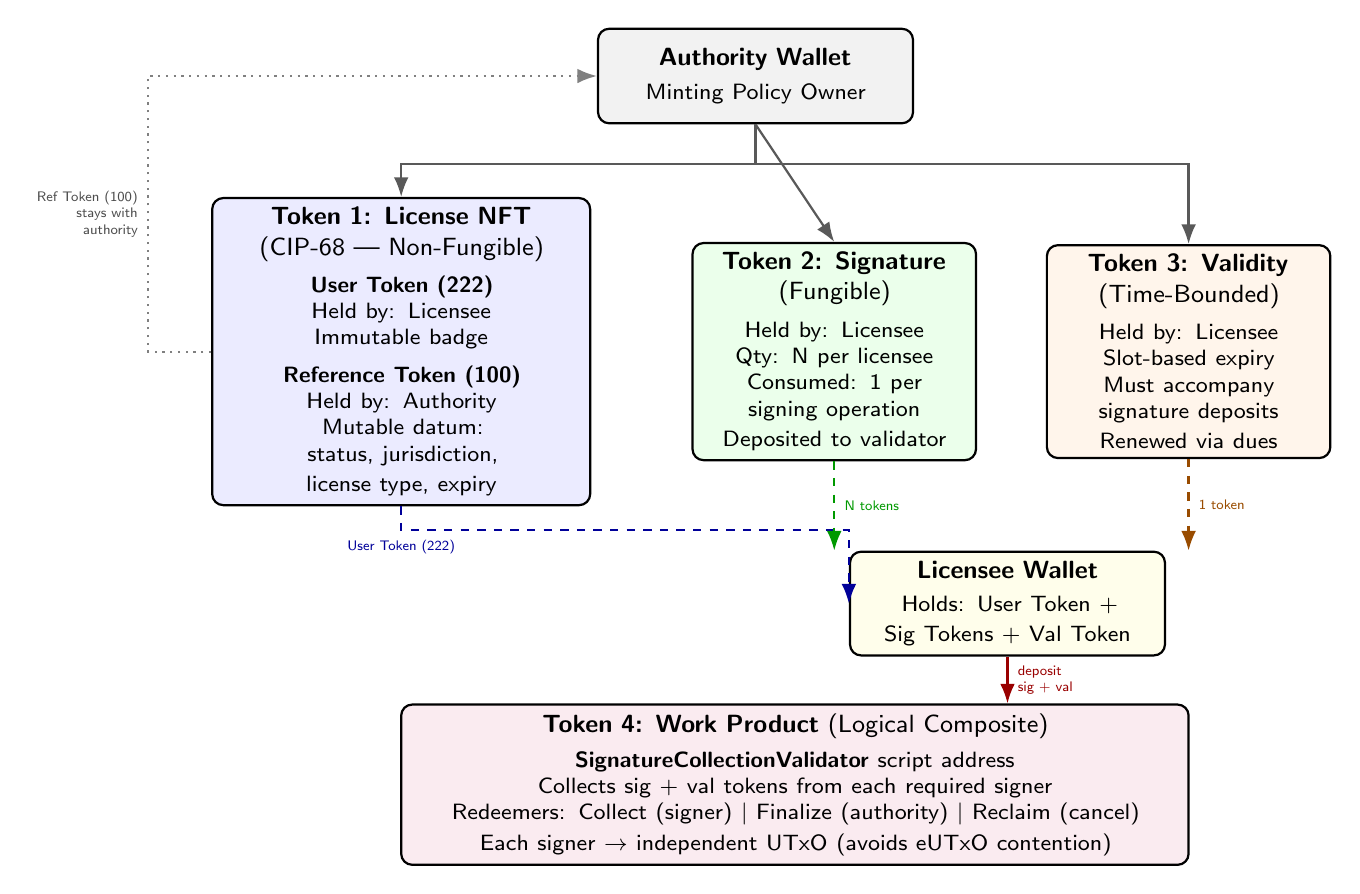
\begin{tikzpicture}[
  guidebox/.style={draw, rounded corners=4pt, thick, align=center, font=\sffamily\small, fill=white, minimum height=1cm},
  guidearrow/.style={-{Latex[length=2.5mm]}, thick, color=gray!70!black},
  guidelabel/.style={font=\sffamily\footnotesize, text=gray!50!black},
]
  % === Authority ===
  \node[guidebox, fill=gray!10, minimum width=4cm, minimum height=1.2cm, text width=3.6cm] (auth) at (0, 9.5)
    {\textbf{Authority Wallet}\\[1pt]\footnotesize Minting Policy Owner};

  % === Token 1: License NFT ===
  \node[guidebox, fill=blue!8, minimum width=4.8cm, minimum height=2.8cm, text width=4.4cm] (licnft) at (-4.5, 6)
    {\textbf{Token 1: License NFT}\\(CIP-68 --- Non-Fungible)\\[4pt]
    \footnotesize \textbf{User Token (222)}\\Held by: Licensee\\Immutable badge\\[4pt]
    \textbf{Reference Token (100)}\\Held by: Authority\\Mutable datum:\\status, jurisdiction,\\license type, expiry};

  % === Token 2: Signature Token ===
  \node[guidebox, fill=green!8, minimum width=3.6cm, minimum height=2.2cm, text width=3.2cm] (sigtok) at (1, 6)
    {\textbf{Token 2: Signature}\\(Fungible)\\[4pt]
    \footnotesize Held by: Licensee\\Qty: N per licensee\\Consumed: 1 per\\signing operation\\Deposited to validator};

  % === Token 3: Validity Token ===
  \node[guidebox, fill=orange!8, minimum width=3.6cm, minimum height=2.2cm, text width=3.2cm] (valtok) at (5.5, 6)
    {\textbf{Token 3: Validity}\\(Time-Bounded)\\[4pt]
    \footnotesize Held by: Licensee\\Slot-based expiry\\Must accompany\\signature deposits\\Renewed via dues};

  % === Licensee Wallet ===
  \node[guidebox, fill=yellow!8, minimum width=4cm, minimum height=1cm, text width=3.6cm] (licensee) at (3.2, 2.8)
    {\textbf{Licensee Wallet}\\[1pt]\footnotesize Holds: User Token + Sig Tokens + Val Token};

  % === Token 4: Work Product / Validator ===
  \node[guidebox, fill=purple!8, minimum width=10cm, minimum height=1.8cm, text width=9.5cm] (wp) at (0.5, 0.5)
    {\textbf{Token 4: Work Product} (Logical Composite)\\[3pt]
    \footnotesize \textbf{SignatureCollectionValidator} script address\\
    Collects sig + val tokens from each required signer\\
    Redeemers: Collect (signer) $|$ Finalize (authority) $|$ Reclaim (cancel)\\
    Each signer $\to$ independent UTxO (avoids eUTxO contention)};

  % === Arrows: Authority mints ===
  \draw[guidearrow] (auth.south) -- ++(0,-0.5) -| (licnft.north);
  \draw[guidearrow] (auth.south) -- (sigtok.north);
  \draw[guidearrow] (auth.south) -- ++(0,-0.5) -| (valtok.north);

  % === Arrows: Tokens to licensee ===
  \draw[guidearrow, dashed, blue!60!black] (licnft.south) -- ++(0,-0.3)
    node[below, font=\sffamily\tiny, text=blue!60!black] {User Token (222)} -| (licensee.west);
  \draw[guidearrow, dashed, green!60!black] (sigtok.south) --
    node[right, font=\sffamily\tiny, text=green!60!black] {N tokens} (licensee.north -| sigtok);
  \draw[guidearrow, dashed, orange!60!black] (valtok.south) --
    node[right, font=\sffamily\tiny, text=orange!60!black] {1 token} (licensee.north -| valtok);

  % === Arrows: Licensee deposits to validator ===
  \draw[guidearrow, thick, red!60!black] (licensee.south) -- node[right, font=\sffamily\tiny, text=red!60!black, align=left] {deposit\\sig + val} (wp.north -| licensee);

  % === Note: Ref Token stays with authority ===
  \draw[guidearrow, dotted, gray] (licnft.west) -- ++(-0.8, 0) |- (auth.west)
    node[pos=0.25, left, font=\sffamily\tiny, text=gray!60!black, align=right] {Ref Token (100)\\stays with\\authority};

\end{tikzpicture}
\caption{Token taxonomy showing all four token types, their holders, and their flow through the system. The authority mints all tokens. The licensee receives the User Token (222), signature tokens, and validity tokens. Signing deposits sig+val tokens into the SignatureCollectionValidator. The Reference Token (100) remains with the authority for status updates.}
\label{fig:ch5-tokens}
\end{figure}


% ============================================================================
\section{Wallet Roles}
\label{sec:ch5-wallets}

The system defines four wallet roles, each with distinct permissions and key storage requirements. This role separation is not merely organizational---it is enforced on-chain by minting policies (which check for the authority's key) and by validator scripts (which check for specific signer public key hashes). A wallet's role determines what transactions it can construct and sign.

\subsection{Authority}

The authority wallet belongs to the licensing board, professional association, or credentialing body. It is the most privileged role in the system. The authority can \textbf{mint and burn all token types} (license NFTs, signature tokens, validity tokens), \textbf{create minting policies} (the native scripts that restrict minting to the authority's key), and \textbf{deploy validator scripts} (the Plutus V2 scripts that manage signature collection and dues enforcement). The authority also controls the Reference Token (label 100) of every CIP-68 license NFT it has issued, giving it unilateral revocation power.

Because the authority key can mint tokens that represent professional credentials, its compromise would be catastrophic: an attacker could issue fraudulent licenses. For this reason, authority keys are stored \textbf{server-side with AES-256-GCM encryption}, protected by restrictive file permissions, and ideally backed by hardware security modules in production. The migration path to multi-signature governance (3-of-5 \texttt{ScriptNofK} or KERI AID delegation) distributes this trust across multiple key holders, but the single-key model is the current implementation.

\subsection{Licensee}

The licensee is the professional---the engineer, physician, attorney, or other credentialed individual. The licensee \textbf{holds the license NFT User Token (222)} in their personal wallet, \textbf{receives and deposits signature and validity tokens} during signing ceremonies, and \textbf{pays dues} to the authority's dues enforcement contract.

Critically, the licensee wallet uses a \textbf{CIP-30 non-custodial model}. The system never has access to the licensee's private keys. Instead, the licensee connects a standard Cardano browser wallet (Eternl, Nami, or Lace) to the system's web interface. When a transaction requires the licensee's signature---for example, depositing tokens into a validator---the application constructs the transaction and sends it to the CIP-30 wallet for signing. The licensee reviews and approves the transaction in their wallet extension. This is the same pattern used by all Cardano DeFi applications and means that the system cannot spend the licensee's tokens without their explicit consent.

\subsection{Signer}

The signer role is functionally similar to the licensee role but is used specifically in the context of multi-party signing ceremonies. A signer \textbf{deposits signature and validity tokens} into the \texttt{SignatureCollectionValidator} to attest to a work product. Like the licensee, the signer uses a \textbf{CIP-30 non-custodial wallet} and retains full control of their private keys.

In many cases, the licensee and signer are the same entity---a PE signing their own drawings is both licensee (they hold the license) and signer (they deposit tokens into the validator). The role distinction matters primarily in multi-party scenarios where different individuals contribute signatures to the same work product, each with their own license NFT and token balances.

\subsection{Observer}

The observer is any third party that needs to verify a credential but does not need to create, hold, or transfer tokens. Observers have \textbf{read-only access}: they can query the blockchain (via Blockfrost or any other chain indexer) to check whether a license NFT exists, whether its Reference Token datum shows \texttt{status: active}, and whether the policy ID matches a registered authority. Observers need only a \textbf{public key}---no private key, no wallet software, no account.

The observer role is what makes the system publicly verifiable. A hospital verifying a physician's license, a building department checking an engineer's credentials, or a client confirming an attorney's bar membership all act as observers. The verification is permissionless: no registration, no API key, no bilateral agreement with the issuing authority is required.

\begin{figure}[htbp]
\centering
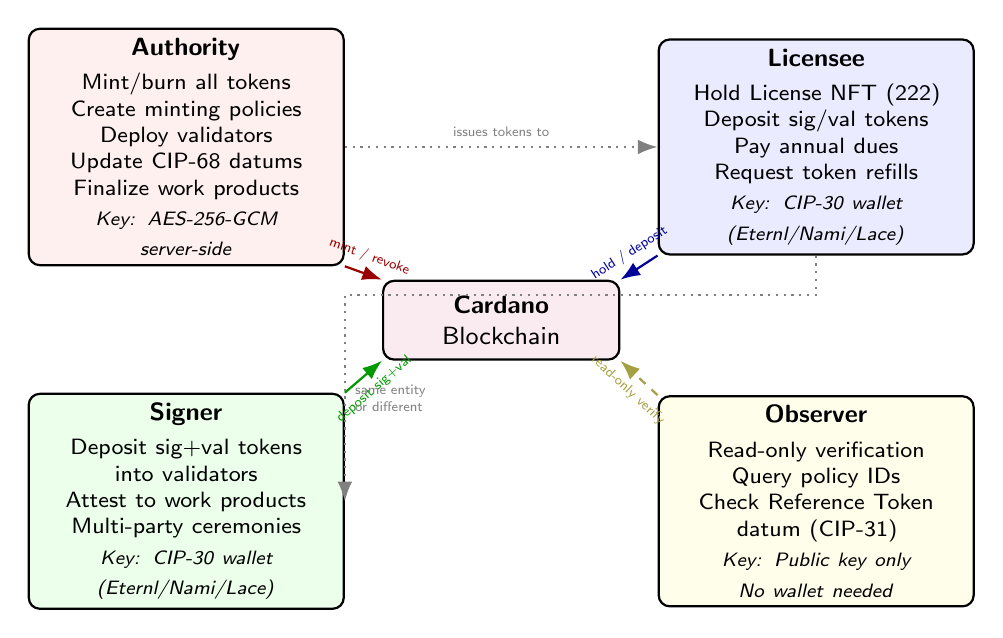
\begin{tikzpicture}[
  guidebox/.style={draw, rounded corners=4pt, thick, align=center, font=\sffamily\small, fill=white, minimum height=1cm},
  guidearrow/.style={-{Latex[length=2.5mm]}, thick, color=gray!70!black},
  guidelabel/.style={font=\sffamily\footnotesize, text=gray!50!black},
]
  % === Four Roles ===
  \node[guidebox, fill=red!6, minimum width=4cm, minimum height=2.4cm, text width=3.6cm] (authority) at (-4, 4)
    {\textbf{Authority}\\[3pt]
    \footnotesize Mint/burn all tokens\\Create minting policies\\Deploy validators\\Update CIP-68 datums\\Finalize work products\\[3pt]
    \scriptsize \textit{Key: AES-256-GCM\\server-side}};

  \node[guidebox, fill=blue!8, minimum width=4cm, minimum height=2.4cm, text width=3.6cm] (licensee) at (4, 4)
    {\textbf{Licensee}\\[3pt]
    \footnotesize Hold License NFT (222)\\Deposit sig/val tokens\\Pay annual dues\\Request token refills\\[3pt]
    \scriptsize \textit{Key: CIP-30 wallet\\(Eternl/Nami/Lace)}};

  \node[guidebox, fill=green!8, minimum width=4cm, minimum height=2.4cm, text width=3.6cm] (signer) at (-4, -0.5)
    {\textbf{Signer}\\[3pt]
    \footnotesize Deposit sig+val tokens\\into validators\\Attest to work products\\Multi-party ceremonies\\[3pt]
    \scriptsize \textit{Key: CIP-30 wallet\\(Eternl/Nami/Lace)}};

  \node[guidebox, fill=yellow!8, minimum width=4cm, minimum height=2.4cm, text width=3.6cm] (observer) at (4, -0.5)
    {\textbf{Observer}\\[3pt]
    \footnotesize Read-only verification\\Query policy IDs\\Check Reference Token\\datum (CIP-31)\\[3pt]
    \scriptsize \textit{Key: Public key only\\No wallet needed}};

  % === Central: Blockchain ===
  \node[guidebox, fill=purple!8, minimum width=3cm, minimum height=1cm, text width=2.6cm] (chain) at (0, 1.8)
    {\textbf{Cardano}\\Blockchain};

  % === Arrows ===
  \draw[guidearrow, red!60!black] (authority.south east) -- node[above, font=\sffamily\tiny, sloped] {mint / revoke} (chain.north west);
  \draw[guidearrow, blue!60!black] (licensee.south west) -- node[above, font=\sffamily\tiny, sloped] {hold / deposit} (chain.north east);
  \draw[guidearrow, green!60!black] (signer.north east) -- node[below, font=\sffamily\tiny, sloped] {deposit sig+val} (chain.south west);
  \draw[guidearrow, dashed, yellow!60!black] (observer.north west) -- node[below, font=\sffamily\tiny, sloped] {read-only verify} (chain.south east);

  % === Inter-role arrows ===
  \draw[guidearrow, dotted, gray] (authority.east) -- node[above, font=\sffamily\tiny] {issues tokens to} (licensee.west);
  \draw[guidearrow, dotted, gray] (licensee.south) -- ++(0,-0.5) -| node[near end, right, font=\sffamily\tiny, align=left] {same entity\\or different} (signer.east);

\end{tikzpicture}
\caption{Four wallet roles and their interactions with the Cardano blockchain. The authority has full mint/burn privileges with server-side key storage. Licensees and signers use non-custodial CIP-30 wallets. Observers perform read-only verification with no wallet required.}
\label{fig:ch5-roles}
\end{figure}


% ============================================================================
\section{Credential Lifecycle}
\label{sec:ch5-lifecycle}

A credential moves through eight distinct steps from creation to verification (and potentially revocation). Each step involves specific participants, specific transactions, and specific on-chain effects. This section traces the full journey in detail.

\subsection{Step (a): Policy Creation}

Before any tokens can be minted, the authority creates a \textbf{minting policy}. In this system, the minting policy is a \textbf{native script}---specifically, a \texttt{ScriptPubkey} that requires the authority's payment verification key hash. The policy script is serialized, and its Blake2b-224 hash becomes the \textbf{Policy ID}, a 28-byte identifier that uniquely and deterministically identifies all tokens minted under this policy.

The Policy ID is critical for verification. When a third party sees a license NFT in someone's wallet, the first thing they check is the Policy ID. If the Policy ID matches one registered to a known licensing board, the token is legitimate (it could only have been minted by someone who controls the authority's private key). If the Policy ID is unknown, the token is either fraudulent or from an unrecognized authority. This is analogous to checking the seal on a physical certificate---except that forging a Policy ID requires forging an Ed25519 private key, which is computationally infeasible.

The policy creation step is a one-time operation per authority. The resulting Policy ID is published, registered, and used for all subsequent minting operations. No on-chain transaction is required to create the policy itself---the policy exists as a serialized script that is included in minting transactions.

\subsection{Step (b): License NFT Minting (CIP-68)}

The authority constructs a minting transaction that creates two tokens simultaneously under the same Policy ID:

\begin{enumerate}[nosep]
  \item The \textbf{Reference Token (label 100)} is sent to the authority's own UTxO. Its inline datum contains the credential metadata:
  \begin{itemize}[nosep]
    \item \texttt{license\_type}: ``PE'', ``MD'', ``JD'', etc.
    \item \texttt{jurisdiction}: ``US-CA'', ``US-NY'', etc.
    \item \texttt{issue\_date}: ISO 8601 date string
    \item \texttt{licensee\_identity}: public key hash of the licensee
    \item \texttt{status}: ``active'' (initial value)
  \end{itemize}
  \item The \textbf{User Token (label 222)} is sent to the licensee's wallet address. This token has the same Policy ID and base asset name as the Reference Token, differing only in the CIP-68 label prefix.
\end{enumerate}

The transaction includes the native script as a witness and is signed by the authority's payment signing key. Upon confirmation, the licensee's wallet shows the User Token, and the authority's address holds the Reference Token with its inline datum. The total cost is approximately 2.2 ADA (0.2 ADA transaction fee + 2.0 ADA minimum UTxO deposit for the Reference Token).

\subsection{Step (c): Signature and Validity Token Minting}

In a separate transaction (or batched into the same transaction for efficiency), the authority mints \textbf{signature tokens} and a \textbf{validity token} for the licensee. Signature tokens are minted in a batch---typically 100 at a time---under the same Policy ID. The validity token is minted with an asset name or datum encoding its expiry slot. Both are sent to the licensee's wallet address. The cost is approximately 2.2 ADA per batch.

\subsection{Step (d): Token Holding}

The licensee now holds three types of tokens in their CIP-30 wallet: the User Token (222), a balance of signature tokens, and a validity token. These tokens are visible in any Cardano wallet that supports native assets. The licensee can see their token balances, verify the Policy ID, and confirm that the tokens are genuine. No further action is required until the licensee needs to sign a document or renew their validity.

\subsection{Step (e): Signing (Token Deposit)}

When the licensee (acting as a signer) needs to sign a document, they deposit one signature token and one validity token into the \texttt{SignatureCollectionValidator} script address. The transaction includes a \texttt{SignerDatum} containing:

\begin{itemize}[nosep]
  \item The signer's public key hash (PKH)
  \item The SHA-256 hash of the document being signed
  \item The Policy ID of the signer's license
  \item The validity token's expiry slot
  \item The current slot (deposit timestamp)
\end{itemize}

The validator script checks that: (1) the signature token has the correct Policy ID, (2) the validity token has the correct Policy ID and its expiry slot is in the future, and (3) the transaction is signed by the signer whose PKH is in the datum. If all checks pass, the transaction is accepted, and the tokens are locked at the script address. Each signer creates an \textbf{independent UTxO} at the script address, avoiding the eUTxO contention problem that would arise if all signers tried to spend the same UTxO.

\subsection{Step (f): Verification}

Any observer can verify the signing event by querying the validator script address and checking the UTxOs. The verification process (detailed in Section~\ref{sec:ch5-verification}) confirms that tokens with the correct Policy ID are present at the validator address, that the Policy ID maps to a registered authority, that the Reference Token datum shows \texttt{status: active}, and that the validity token had not expired at the time of deposit. This verification can be performed by anyone, at any time, without permission from any party.

\subsection{Step (g): Renewal}

When the validity token approaches expiry, the licensee pays dues to the authority's \textbf{dues enforcement contract}. This Plutus V2 contract verifies that the correct ADA amount was paid and that the payment is within the grace period. Upon successful payment, the authority mints a new validity token with an updated expiry slot and sends it to the licensee's wallet. The old validity token is either burned or simply becomes useless (its expiry slot is in the past, so no validator will accept it).

The renewal process creates a direct economic link between professional standing and signing capacity. If a licensee fails to pay dues, their validity token expires, and they cannot sign documents---even though they still hold the User Token (222) and may have remaining signature tokens. This mirrors real-world licensing: a PE whose license lapses due to unpaid dues cannot legally stamp drawings, even though they once held a valid license.

\subsection{Step (h): Revocation}

If the authority needs to revoke a credential (due to disciplinary action, fraud, or other cause), it updates the Reference Token's inline datum to \texttt{status: revoked}. This is a simple transaction: the authority spends the UTxO holding the Reference Token and creates a new UTxO at the same address with the same token but an updated datum. The transaction costs approximately 0.3 ADA and requires only the authority's signature.

The revocation is effective immediately upon confirmation (within approximately 20 seconds for the first block, with practical finality in approximately 5 minutes). Any subsequent verification will read the Reference Token's datum and find \texttt{status: revoked}. The User Token (222) remains in the licensee's wallet, but it is now meaningless---a verified credential requires both the User Token \emph{and} an active Reference Token datum. This mechanism is detailed in Section~\ref{sec:ch5-revocation}.

\begin{figure}[p]
\centering
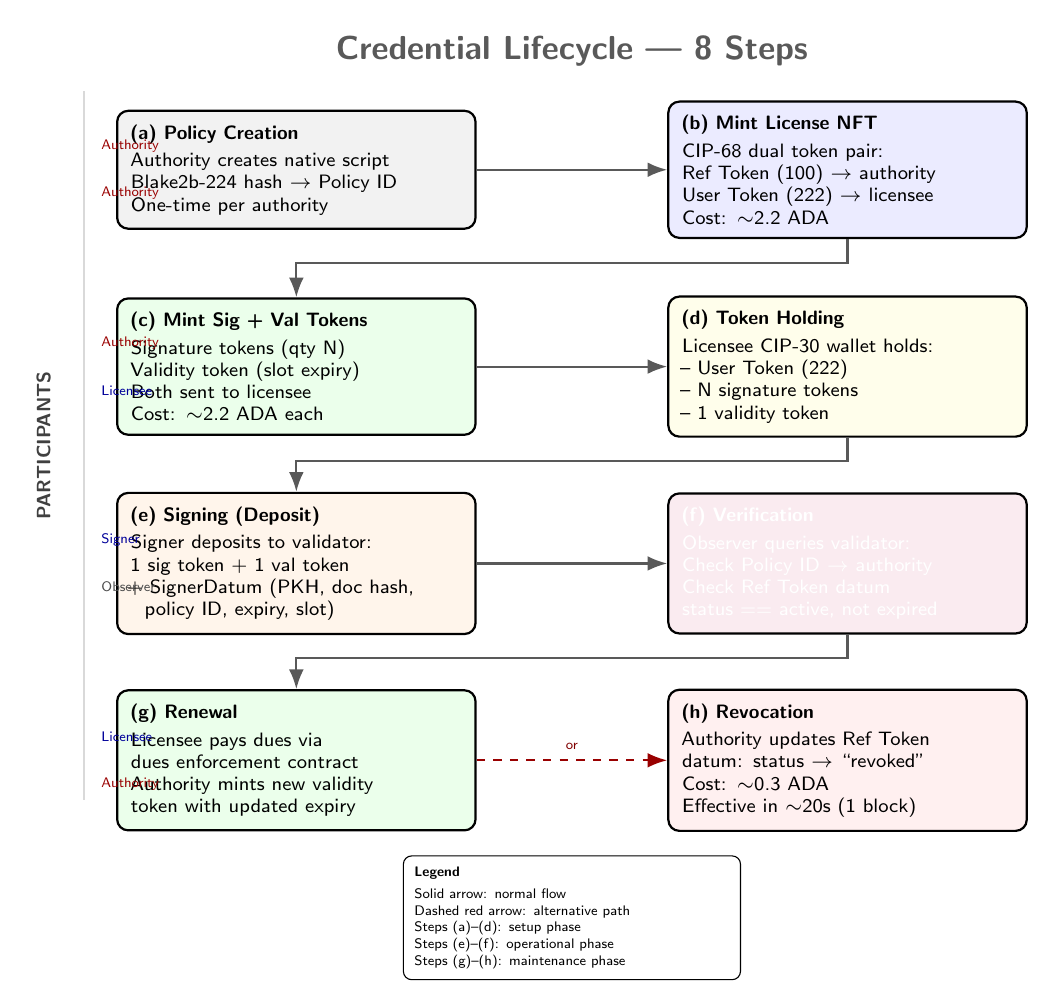
\begin{tikzpicture}[
  guidebox/.style={draw, rounded corners=4pt, thick, align=center, font=\sffamily\small, fill=white, minimum height=1cm},
  guidearrow/.style={-{Latex[length=2.5mm]}, thick, color=gray!70!black},
  guidelabel/.style={font=\sffamily\footnotesize, text=gray!50!black},
  stepbox/.style={draw, rounded corners=4pt, thick, align=left, font=\sffamily\scriptsize, fill=white, minimum height=1.4cm, text width=4.2cm, inner sep=5pt},
]
  % Title
  \node[font=\sffamily\large\bfseries, text=gray!70!black] at (0, 15.5) {Credential Lifecycle --- 8 Steps};

  % === Step (a) ===
  \node[stepbox, fill=gray!10] (stepa) at (-3.5, 14)
    {\textbf{(a) Policy Creation}\\[2pt]
    Authority creates native script\\
    Blake2b-224 hash $\to$ Policy ID\\
    One-time per authority};

  % === Step (b) ===
  \node[stepbox, fill=blue!8] (stepb) at (3.5, 14)
    {\textbf{(b) Mint License NFT}\\[2pt]
    CIP-68 dual token pair:\\
    Ref Token (100) $\to$ authority\\
    User Token (222) $\to$ licensee\\
    Cost: $\sim$2.2 ADA};

  % === Step (c) ===
  \node[stepbox, fill=green!8] (stepc) at (-3.5, 11.5)
    {\textbf{(c) Mint Sig + Val Tokens}\\[2pt]
    Signature tokens (qty N)\\
    Validity token (slot expiry)\\
    Both sent to licensee\\
    Cost: $\sim$2.2 ADA each};

  % === Step (d) ===
  \node[stepbox, fill=yellow!8] (stepd) at (3.5, 11.5)
    {\textbf{(d) Token Holding}\\[2pt]
    Licensee CIP-30 wallet holds:\\
    -- User Token (222)\\
    -- N signature tokens\\
    -- 1 validity token};

  % === Step (e) ===
  \node[stepbox, fill=orange!8] (stepe) at (-3.5, 9)
    {\textbf{(e) Signing (Deposit)}\\[2pt]
    Signer deposits to validator:\\
    1 sig token + 1 val token\\
    + SignerDatum (PKH, doc hash,\\
    \ \ policy ID, expiry, slot)};

  % === Step (f) ===
  \node[stepbox, fill=purple!8, text=white] (stepf) at (3.5, 9)
    {\textbf{(f) Verification}\\[2pt]
    Observer queries validator:\\
    Check Policy ID $\to$ authority\\
    Check Ref Token datum\\
    status == active, not expired};

  % === Step (g) ===
  \node[stepbox, fill=green!8] (stepg) at (-3.5, 6.5)
    {\textbf{(g) Renewal}\\[2pt]
    Licensee pays dues via\\
    dues enforcement contract\\
    Authority mints new validity\\
    token with updated expiry};

  % === Step (h) ===
  \node[stepbox, fill=red!6] (steph) at (3.5, 6.5)
    {\textbf{(h) Revocation}\\[2pt]
    Authority updates Ref Token\\
    datum: status $\to$ ``revoked''\\
    Cost: $\sim$0.3 ADA\\
    Effective in $\sim$20s (1 block)};

  % === Arrows ===
  \draw[guidearrow] (stepa.east) -- (stepb.west);
  \draw[guidearrow] (stepb.south) -- ++(0, -0.3) -| (stepc.north);
  \draw[guidearrow] (stepc.east) -- (stepd.west);
  \draw[guidearrow] (stepd.south) -- ++(0, -0.3) -| (stepe.north);
  \draw[guidearrow] (stepe.east) -- (stepf.west);
  \draw[guidearrow] (stepf.south) -- ++(0, -0.3) -| (stepg.north);
  \draw[guidearrow, dashed, red!60!black] (stepg.east) -- node[above, font=\sffamily\tiny, text=red!50!black] {or} (steph.west);

  % === Participants sidebar ===
  \node[font=\sffamily\scriptsize\bfseries, text=gray!50!black, rotate=90, anchor=south] at (-6.5, 10.5) {PARTICIPANTS};
  \draw[thick, gray!30] (-6.2, 6) -- (-6.2, 15);

  \node[font=\sffamily\tiny, text=red!60!black, anchor=west] at (-6.1, 14.3) {Authority};
  \node[font=\sffamily\tiny, text=red!60!black, anchor=west] at (-6.1, 13.7) {Authority};
  \node[font=\sffamily\tiny, text=red!60!black, anchor=west] at (-6.1, 11.8) {Authority};
  \node[font=\sffamily\tiny, text=blue!60!black, anchor=west] at (-6.1, 11.2) {Licensee};
  \node[font=\sffamily\tiny, text=blue!60!black, anchor=west] at (-6.1, 9.3) {Signer};
  \node[font=\sffamily\tiny, text=gray!60!black, anchor=west] at (-6.1, 8.7) {Observer};
  \node[font=\sffamily\tiny, text=blue!60!black, anchor=west] at (-6.1, 6.8) {Licensee};
  \node[font=\sffamily\tiny, text=red!60!black, anchor=west] at (-6.1, 6.2) {Authority};

  % === Legend ===
  \node[draw, rounded corners=3pt, fill=white, inner sep=4pt, font=\sffamily\tiny, text width=4cm, align=left]
    at (0, 4.5) {
    \textbf{Legend}\\[2pt]
    Solid arrow: normal flow\\
    Dashed red arrow: alternative path\\
    Steps (a)--(d): setup phase\\
    Steps (e)--(f): operational phase\\
    Steps (g)--(h): maintenance phase
    };

\end{tikzpicture}
\caption{Complete credential lifecycle showing all eight steps from policy creation through revocation. The setup phase (a--d) is performed once per credential. The operational phase (e--f) repeats for each signing event. The maintenance phase (g--h) occurs periodically or as needed.}
\label{fig:ch5-lifecycle}
\end{figure}


% ============================================================================
\section{Revocation Mechanism}
\label{sec:ch5-revocation}

This is the most important architectural decision in the entire system. Revocation---the ability for an authority to invalidate a previously issued credential---is the feature that separates a useful credential system from a toy. If a physician loses their license, if an engineer commits fraud, if an attorney is disbarred, the credential must become invalid \emph{immediately and globally}. This section explains why revocation is hard on Cardano, why the naive approach fails, and how the CIP-68 pattern solves the problem.

\subsection{The Problem: eUTxO Ownership}

In Cardano's extended UTxO model, every token sits inside a UTxO, and every UTxO is controlled by either an address (requiring the owner's private key to spend) or a script (requiring satisfaction of the script's conditions to spend). This is a feature, not a bug---it is what makes eUTxO secure. But it creates a specific problem for revocation:

\textbf{You cannot spend (or burn) someone else's UTxO without their private key.}

This is an absolute, non-negotiable property of the ledger. The authority cannot construct a transaction that spends the licensee's UTxO because the ledger requires the licensee's signature for that UTxO. The authority does not have the licensee's private key (and should never have it, by the non-custodial design). This means the authority \emph{cannot forcibly remove a token from the licensee's wallet}.

\subsection{The Broken Approach: Direct Token Burn}

The naive approach to revocation is: ``when the authority wants to revoke a license, burn the licensee's NFT.'' This approach fails completely in eUTxO. To burn a token, you must spend the UTxO that contains it. To spend that UTxO, you need the private key that controls the address where it sits. The licensee's token sits at the licensee's address. The authority does not have the licensee's key. Therefore, the authority cannot burn the licensee's token. Period.

One might suggest requiring the licensee to send the token to the authority upon revocation, but this requires the licensee's cooperation---which is precisely what you cannot count on when revoking someone's license for cause. A physician whose license is being revoked for malpractice is unlikely to voluntarily return their credential token.

Another approach might be to hold the token at a script address controlled by the authority rather than at the licensee's personal address. But this defeats the purpose of the credential: the licensee should be able to prove they hold the token, which requires the token to be in their wallet. If the token is at a script address, the licensee does not ``hold'' it in any meaningful sense.

\subsection{The CIP-68 Solution: Datum-Based Revocation}

The CIP-68 standard resolves this tension elegantly by splitting the credential into two tokens with different custody:

\begin{enumerate}[nosep]
  \item The \textbf{User Token (222)} goes to the licensee's wallet. The authority \emph{cannot} touch it. The licensee holds it forever (or until they voluntarily send it somewhere). This is fine because \textbf{the User Token is not the source of truth}.
  \item The \textbf{Reference Token (100)} stays at the authority's UTxO. The authority \emph{can} spend this UTxO at any time because the authority controls the private key for that address. The Reference Token carries an \textbf{inline datum} with a \texttt{status} field.
\end{enumerate}

Revocation is performed by the authority spending the UTxO that holds the Reference Token and creating a new UTxO at the same address with the same Reference Token but an updated datum: \texttt{status: ``revoked''}. This transaction:

\begin{itemize}[nosep]
  \item Requires \textbf{only the authority's signature}---no interaction with the licensee.
  \item Costs approximately \textbf{0.3 ADA} (a simple transaction fee; no Plutus execution needed for a native script policy).
  \item Takes effect within approximately \textbf{20 seconds} (one block confirmation).
  \item Is \textbf{globally visible}---any observer who reads the Reference Token's inline datum will see \texttt{status: revoked}.
\end{itemize}

The User Token (222) in the licensee's wallet is now meaningless. It still exists---the licensee still ``holds'' it---but any verifier performing a proper verification will check the Reference Token's datum and find \texttt{status: revoked}. The User Token without an active Reference Token is like a physical certificate after the issuing board has published a revocation notice: the paper exists, but the credential it represents has been invalidated.

\subsection{The minUTxO Economics}

Every UTxO on Cardano must carry a minimum ADA deposit (approximately 2.0 ADA for a UTxO carrying a native token with an inline datum). This ADA is not ``spent''---it is locked and can be recovered when the UTxO is consumed. When the authority mints the Reference Token, approximately 2.0 ADA is locked at the UTxO. When the authority performs a revocation (spending and re-creating the UTxO with updated datum), the 2.0 ADA remains locked at the new UTxO. If the authority later decides to \textbf{burn the Reference Token entirely} (removing it from the ledger), the locked ADA is returned to the authority's wallet, minus the transaction fee of approximately 0.3 ADA. The net recovery is approximately 1.7 ADA per burned Reference Token.

For a licensing board managing 10,000 licenses, the total locked ADA at Reference Token UTxOs is approximately 20,000 ADA (approximately \$6,000 at \$0.30/ADA). This is the economic cost of maintaining revocable credentials---a modest amount compared to the annual operating budgets of professional licensing boards.

\begin{figure}[htbp]
\centering
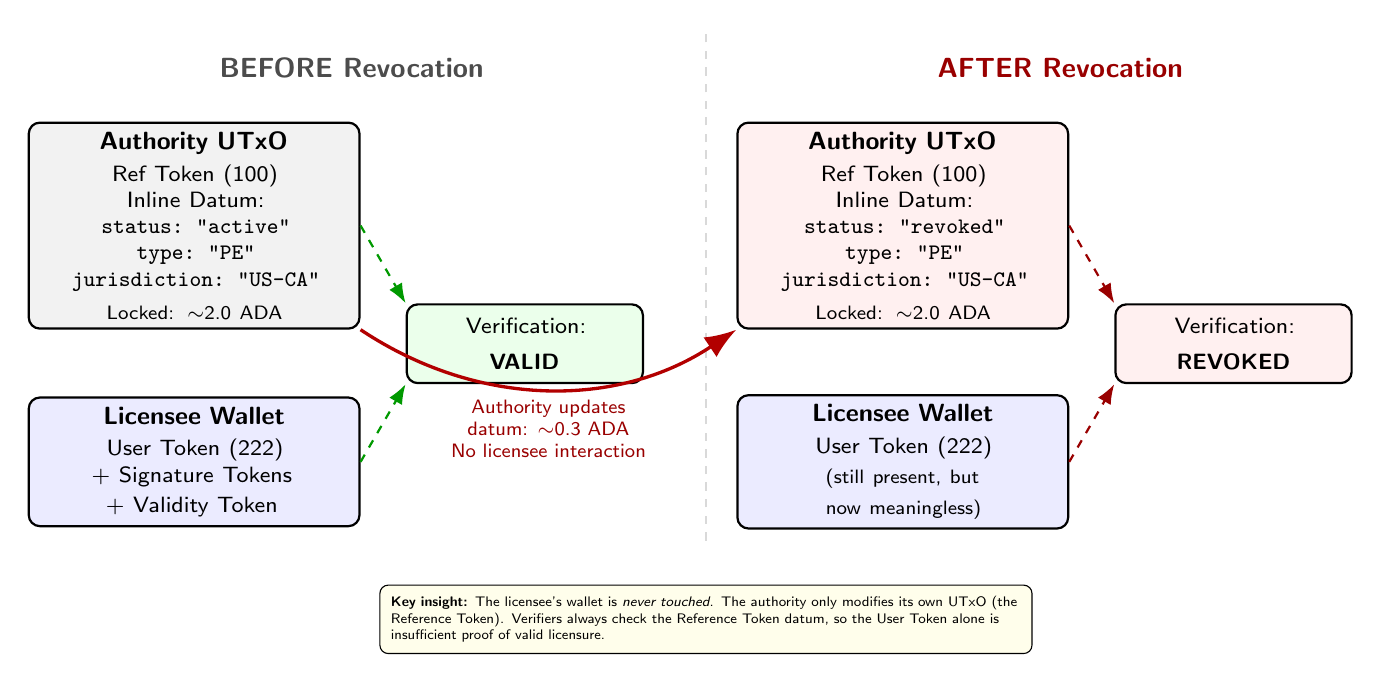
\begin{tikzpicture}[
  guidebox/.style={draw, rounded corners=4pt, thick, align=center, font=\sffamily\small, fill=white, minimum height=1cm},
  guidearrow/.style={-{Latex[length=2.5mm]}, thick, color=gray!70!black},
  guidelabel/.style={font=\sffamily\footnotesize, text=gray!50!black},
]
  % === BEFORE REVOCATION ===
  \node[font=\sffamily\bfseries, text=gray!60!black] at (-4.5, 7.5) {BEFORE Revocation};

  % Authority side - before
  \node[guidebox, fill=gray!10, minimum width=4.2cm, minimum height=1.8cm, text width=3.8cm] (auth_before) at (-6.5, 5.5)
    {\textbf{Authority UTxO}\\[2pt]
    \footnotesize Ref Token (100)\\
    Inline Datum:\\
    \texttt{status: "active"}\\
    \texttt{type: "PE"}\\
    \texttt{jurisdiction: "US-CA"}\\[1pt]
    \scriptsize Locked: $\sim$2.0 ADA};

  % Licensee side - before
  \node[guidebox, fill=blue!8, minimum width=4.2cm, minimum height=1.4cm, text width=3.8cm] (lic_before) at (-6.5, 2.5)
    {\textbf{Licensee Wallet}\\[2pt]
    \footnotesize User Token (222)\\
    + Signature Tokens\\
    + Validity Token};

  % Verification result - before
  \node[guidebox, fill=green!8, minimum width=3cm, text width=2.6cm] (verify_before) at (-2.3, 4)
    {\footnotesize Verification:\\[2pt] \textbf{VALID}};

  \draw[guidearrow, dashed, green!60!black] (auth_before.east) -- (verify_before.north west);
  \draw[guidearrow, dashed, green!60!black] (lic_before.east) -- (verify_before.south west);

  % === Divider ===
  \draw[thick, gray!30, dashed] (0, 1.5) -- (0, 8);

  % === AFTER REVOCATION ===
  \node[font=\sffamily\bfseries, text=red!60!black] at (4.5, 7.5) {AFTER Revocation};

  % Authority side - after
  \node[guidebox, fill=red!6, minimum width=4.2cm, minimum height=1.8cm, text width=3.8cm] (auth_after) at (2.5, 5.5)
    {\textbf{Authority UTxO}\\[2pt]
    \footnotesize Ref Token (100)\\
    Inline Datum:\\
    \texttt{status: "revoked"}\\
    \texttt{type: "PE"}\\
    \texttt{jurisdiction: "US-CA"}\\[1pt]
    \scriptsize Locked: $\sim$2.0 ADA};

  % Licensee side - after (unchanged!)
  \node[guidebox, fill=blue!8, minimum width=4.2cm, minimum height=1.4cm, text width=3.8cm] (lic_after) at (2.5, 2.5)
    {\textbf{Licensee Wallet}\\[2pt]
    \footnotesize User Token (222)\\
    \scriptsize (still present, but now meaningless)};

  % Verification result - after
  \node[guidebox, fill=red!6, minimum width=3cm, text width=2.6cm] (verify_after) at (6.7, 4)
    {\footnotesize Verification:\\[2pt] \textbf{REVOKED}};

  \draw[guidearrow, dashed, red!60!black] (auth_after.east) -- (verify_after.north west);
  \draw[guidearrow, dashed, red!60!black] (lic_after.east) -- (verify_after.south west);

  % === Revocation arrow ===
  \draw[guidearrow, very thick, red!70!black, -{Latex[length=4mm]}]
    (auth_before.south east) .. controls +(1.5, -1) and +(-1.5, -1) ..
    node[below, font=\sffamily\scriptsize, text=red!60!black, align=center]
    {Authority updates\\datum: $\sim$0.3 ADA\\No licensee interaction} (auth_after.south west);

  % === Note ===
  \node[draw, rounded corners=3pt, fill=yellow!8, inner sep=4pt, font=\sffamily\tiny, text width=8cm, align=left]
    at (0, 0.5) {
    \textbf{Key insight:} The licensee's wallet is \emph{never touched}. The authority only modifies
    its own UTxO (the Reference Token). Verifiers always check the Reference Token datum,
    so the User Token alone is insufficient proof of valid licensure.
    };

\end{tikzpicture}
\caption{Before and after revocation. The authority updates only its own Reference Token datum from ``active'' to ``revoked.'' The licensee's User Token remains in their wallet but is now meaningless for verification purposes. No interaction with the licensee is required.}
\label{fig:ch5-revocation}
\end{figure}


% ============================================================================
\section{Verification Flow}
\label{sec:ch5-verification}

Verification is the operation that makes the entire system worthwhile. Everything else---minting, signing, renewal, revocation---exists to produce a state that can be verified. This section describes the exact sequence of steps a third-party observer follows to verify a credential, and explains why each step is necessary.

\subsection{Step-by-Step Verification}

The verification flow consists of seven steps, each building on the previous one. The entire process completes in under 5 seconds, dominated by Blockfrost API latency (200--500ms per query).

\textbf{Step 1: Identify the License NFT.} The verifier obtains the licensee's wallet address (or the licensee presents their wallet via CIP-30). The verifier queries the address's UTxO set and identifies the License NFT User Token (label 222). This step confirms that the licensee holds a token that \emph{claims} to be a license. It does not yet prove anything about the token's legitimacy.

\textbf{Step 2: Extract the Policy ID.} Every Cardano native token has a Policy ID---the Blake2b-224 hash of the minting policy script. The verifier extracts the Policy ID from the User Token. This is a deterministic operation; the Policy ID is part of the token's on-chain identity.

\textbf{Step 3: Verify the Policy ID against a registry.} The verifier checks whether the extracted Policy ID matches any registered authority. This is the step that distinguishes a legitimate credential from a fraudulent one. The registry could be a published list maintained by a standards body, a smart contract on-chain, or a well-known database. If the Policy ID is not recognized, verification fails---the token was minted by an unknown party and cannot be trusted.

\textbf{Step 4: Find the CIP-68 Reference Token.} The verifier constructs the Reference Token's asset name by replacing the User Token's label prefix (222) with the Reference Token's label prefix (100), keeping the same base asset name. The verifier then searches for this Reference Token on-chain. Under CIP-68, the Reference Token should be at a known address (the authority's address or a designated script address).

\textbf{Step 5: Read the inline datum (CIP-31 Reference Input).} Using CIP-31 reference inputs, the verifier reads the Reference Token's inline datum \emph{without spending the UTxO}. This is a read-only operation that does not require any private key and does not create a transaction. The datum contains the credential metadata, including the \texttt{status} field, license type, jurisdiction, issue date, and licensee identity.

\textbf{Step 6: Check status and expiration.} The verifier confirms two conditions: (1) \texttt{status == "active"} (if \texttt{status == "revoked"}, verification fails immediately), and (2) \texttt{expiration > current\_slot} (if the credential has expired, verification fails). The current slot is obtained from the Cardano chain tip.

\textbf{Step 7: Verification complete.} If all checks pass, the credential is verified. The verifier now has cryptographic proof that: the credential was issued by a recognized authority (Policy ID match), the credential is currently active (datum status check), the credential has not expired (slot comparison), and the licensee holds the corresponding User Token (UTxO query).

\begin{figure}[htbp]
\centering
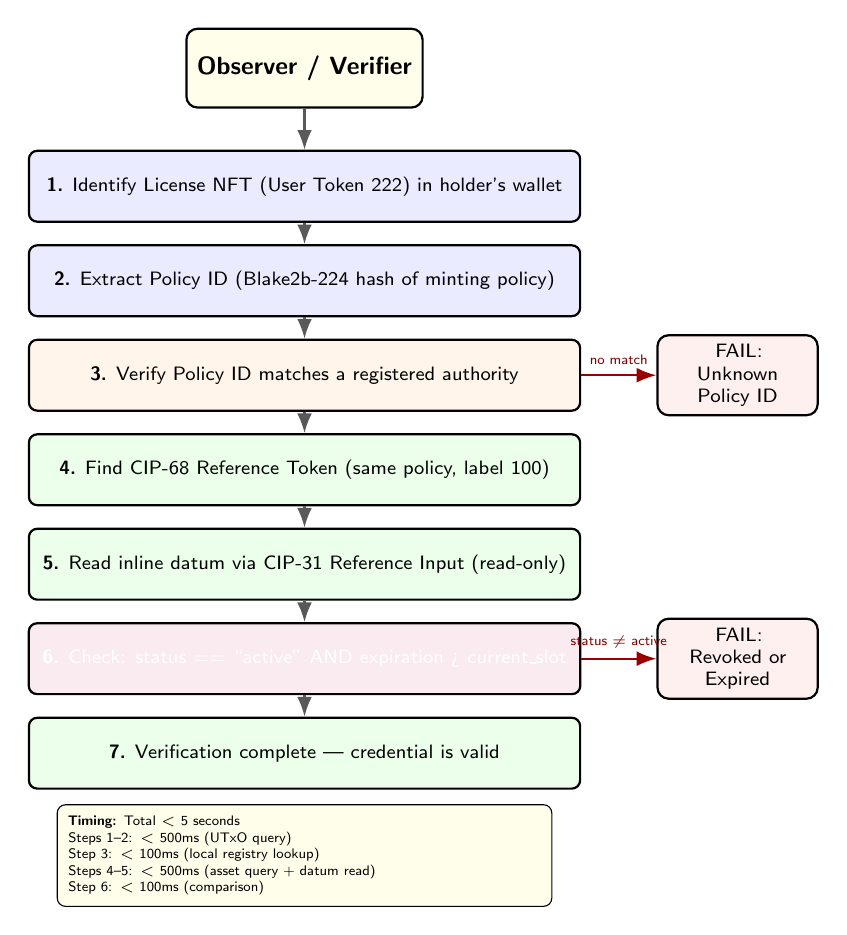
\begin{tikzpicture}[
  guidebox/.style={draw, rounded corners=4pt, thick, align=center, font=\sffamily\small, fill=white, minimum height=1cm},
  guidearrow/.style={-{Latex[length=2.5mm]}, thick, color=gray!70!black},
  guidelabel/.style={font=\sffamily\footnotesize, text=gray!50!black},
  vstep/.style={draw, rounded corners=3pt, thick, fill=white, font=\sffamily\scriptsize, minimum height=0.9cm, minimum width=7cm, align=left, inner sep=5pt},
]
  % === Observer start ===
  \node[guidebox, fill=yellow!8, minimum width=3cm] (observer) at (0, 11.5)
    {\textbf{Observer / Verifier}};

  % === Steps ===
  \node[vstep, fill=blue!8] (s1) at (0, 10)
    {\textbf{1.} Identify License NFT (User Token 222) in holder's wallet};

  \node[vstep, fill=blue!8] (s2) at (0, 8.8)
    {\textbf{2.} Extract Policy ID (Blake2b-224 hash of minting policy)};

  \node[vstep, fill=orange!8] (s3) at (0, 7.6)
    {\textbf{3.} Verify Policy ID matches a registered authority};

  \node[vstep, fill=green!8] (s4) at (0, 6.4)
    {\textbf{4.} Find CIP-68 Reference Token (same policy, label 100)};

  \node[vstep, fill=green!8] (s5) at (0, 5.2)
    {\textbf{5.} Read inline datum via CIP-31 Reference Input (read-only)};

  \node[vstep, fill=purple!8, text=white] (s6) at (0, 4.0)
    {\textbf{6.} Check: status == ``active'' AND expiration > current\_slot};

  \node[vstep, fill=green!8] (s7) at (0, 2.8)
    {\textbf{7.} Verification complete --- credential is valid};

  % === Arrows ===
  \draw[guidearrow] (observer.south) -- (s1.north);
  \draw[guidearrow] (s1.south) -- (s2.north);
  \draw[guidearrow] (s2.south) -- (s3.north);
  \draw[guidearrow] (s3.south) -- (s4.north);
  \draw[guidearrow] (s4.south) -- (s5.north);
  \draw[guidearrow] (s5.south) -- (s6.north);
  \draw[guidearrow] (s6.south) -- (s7.north);

  % === Failure paths ===
  \node[guidebox, fill=red!6, minimum width=2cm, text width=1.8cm, font=\sffamily\scriptsize] (fail1) at (5.5, 7.6)
    {FAIL:\\Unknown\\Policy ID};
  \draw[guidearrow, red!60!black] (s3.east) -- node[above, font=\sffamily\tiny, text=red!50!black] {no match} (fail1.west);

  \node[guidebox, fill=red!6, minimum width=2cm, text width=1.8cm, font=\sffamily\scriptsize] (fail2) at (5.5, 4.0)
    {FAIL:\\Revoked or\\Expired};
  \draw[guidearrow, red!60!black] (s6.east) -- node[above, font=\sffamily\tiny, text=red!50!black] {status $\neq$ active} (fail2.west);

  % === Timing ===
  \node[draw, rounded corners=3pt, fill=yellow!8, inner sep=4pt, font=\sffamily\tiny, text width=6cm, align=left]
    at (0, 1.5) {
    \textbf{Timing:} Total $<$ 5 seconds\\
    Steps 1--2: $<$ 500ms (UTxO query)\\
    Step 3: $<$ 100ms (local registry lookup)\\
    Steps 4--5: $<$ 500ms (asset query + datum read)\\
    Step 6: $<$ 100ms (comparison)
    };

\end{tikzpicture}
\caption{Seven-step verification flow. An observer can verify a credential in under 5 seconds with no permission required. Failure at Step 3 (unknown Policy ID) or Step 6 (revoked/expired status) immediately terminates verification with a negative result.}
\label{fig:ch5-verification}
\end{figure}

\subsection{Permissionless Verification}

A crucial property of this verification flow is that it is \textbf{permissionless}. The observer does not need:

\begin{itemize}[nosep]
  \item An account or API key with the issuing authority
  \item A bilateral trust agreement with any party
  \item Any special software beyond a Blockfrost API client (or any Cardano chain indexer)
  \item The licensee's cooperation (the on-chain state is public)
\end{itemize}

This is fundamentally different from current verification infrastructure, where a hospital must contact the specific state medical board, provide credentials, wait for a response, and trust that the board's database is accurate and current. In the blockchain-based system, the verification is mathematical: the Policy ID either matches or it does not, the datum either shows ``active'' or it does not, and the expiration either exceeds the current slot or it does not.

\subsection{Verification Without a Full Node}

The verification flow described above uses the Blockfrost API, which means the verifier trusts Blockfrost to return accurate chain data. For higher-assurance verification, the observer can run their own Cardano node and query the ledger directly, eliminating all third-party trust. For an intermediate assurance level, Mithril snapshot proofs (planned for 2026) will allow light clients to verify chain state with cryptographic proofs without running a full node.


% ============================================================================
\section{Cost Economics}
\label{sec:ch5-costs}

Understanding the on-chain costs is essential for evaluating the system's economic viability. Every Cardano transaction has two cost components: the \textbf{transaction fee} (paid to stake pool operators, approximately 0.17--0.30 ADA depending on transaction size and Plutus execution) and the \textbf{minimum UTxO deposit} (ADA locked at the output UTxO, recoverable when the UTxO is consumed, approximately 1.5--2.0 ADA depending on the datum and token payload). The table below summarizes costs for each operation.

\begin{table}[htbp]
\centering
\caption{On-chain cost breakdown for credential operations}
\label{tab:ch5-costs}
\small
\begin{tabular}{@{}p{4.5cm}ccc@{}}
\toprule
\textbf{Operation} & \textbf{Tx Fee (ADA)} & \textbf{minUTxO (ADA)} & \textbf{Total (ADA)} \\
\midrule
Mint License NFT (CIP-68 pair) & $\sim$0.2 & $\sim$2.0 & $\sim$2.2 \\
Mint Signature Tokens (batch of 100) & $\sim$0.2 & $\sim$2.0 & $\sim$2.2 \\
Mint Validity Token & $\sim$0.2 & $\sim$2.0 & $\sim$2.2 \\
Sign Document (deposit to validator) & $\sim$0.2 & $\sim$2.0 & $\sim$2.2 \\
Finalize Work Product (Plutus V2) & $\sim$0.3 & $\sim$2.0 & $\sim$2.3 \\
Revoke License (datum update) & $\sim$0.3 & 0\textsuperscript{$\dagger$} & $\sim$0.3 \\
Renew Validity (new token mint) & $\sim$0.2 & $\sim$2.0 & $\sim$2.2 + dues \\
Burn Reference Token (cleanup) & $\sim$0.3 & $-$2.0\textsuperscript{$\ddagger$} & net $\sim$$-$1.7 \\
\bottomrule
\end{tabular}

\vspace{4pt}
\footnotesize
\textsuperscript{$\dagger$}Revocation modifies the existing Reference Token UTxO in place; the $\sim$2.0 ADA deposit remains locked.\\
\textsuperscript{$\ddagger$}Burning the Reference Token releases the locked minUTxO, yielding a net refund of $\sim$1.7 ADA after fees.
\end{table}

\subsection{Comparison to Ethereum}

The same operations on Ethereum would cost significantly more due to the ERC-721 contract execution model. Minting an NFT on Ethereum requires deploying or interacting with a smart contract, with gas costs that vary dramatically based on network congestion. During periods of high activity, gas prices have exceeded 500 gwei, pushing a single NFT mint above \$100. Even at moderate gas prices, a typical ERC-721 mint costs \$1--15, and complex operations like multi-party signature collection (requiring multiple contract calls and state updates) can cost \$5--50 per operation. Cardano's deterministic fee model eliminates this variability entirely: the cost of a transaction is known before submission and does not change based on network load.

Solana offers lower absolute costs (sub-\$0.01 per transaction) but with a different risk profile: multiple network outages, a proof-of-history consensus mechanism with less formal verification than Ouroboros, and a programming model (Rust-based programs) less suited to formal verification of credential logic.

\subsection{Annual Cost Projection}

For a deployment managing 10,000 professional licenses with standard operational assumptions (one license mint per licensee, 100 signature tokens per licensee per year, one validity renewal per year, 10 signing operations per licensee per year), the annual on-chain costs at current ADA prices (\$0.30/ADA) are:

\begin{table}[htbp]
\centering
\caption{Annual cost projection for 10,000 licenses at \$0.30/ADA}
\label{tab:ch5-annual}
\small
\begin{tabular}{@{}p{5cm}cc@{}}
\toprule
\textbf{Category} & \textbf{ADA} & \textbf{USD} \\
\midrule
Initial license minting (one-time, year 1) & 22,000 & \$6,600 \\
Signature token minting (annual batch) & 22,000 & \$6,600 \\
Validity token renewal (annual) & 22,000 & \$6,600 \\
Signing operations (100,000/year) & 220,000 & \$66,000 \\
Revocations (est. 2\% = 200/year) & 60 & \$18 \\
\midrule
\textbf{Year 1 Total} & \textbf{286,060} & \textbf{\$85,818} \\
\textbf{Recurring Annual} & \textbf{264,060} & \textbf{\$79,218} \\
\bottomrule
\end{tabular}

\vspace{4pt}
\footnotesize
Note: The bulk of the cost is signing operations. If each licensee performs only 1 signing per year (as in annual license renewal), the recurring cost drops to approximately \$6,300--8,400 annually. Verification queries are free (read-only Blockfrost API calls). Hydra state-channel batching (2026 roadmap) could reduce signing costs by 90\%+.
\end{table}

The key economic insight is that \textbf{verification is free}. Reading on-chain state through Blockfrost or any chain indexer does not require a transaction and incurs no ADA cost. The current verification infrastructure charges \$5--25 per query (FSMB, Nursys, NCEES verification services). For an organization performing thousands of verifications annually, the savings from free verification alone can offset the entire on-chain transaction cost.

\subsection{Locked ADA and Capital Efficiency}

The minUTxO requirement means that ADA is locked at token-carrying UTxOs. For 10,000 licenses, approximately 20,000 ADA ($\sim$\$6,000) is locked at Reference Token UTxOs, plus additional ADA locked at signature and validity token UTxOs held by licensees. This locked ADA is not lost---it can be recovered by consuming the UTxOs---but it represents an opportunity cost. CIP-68 datum patterns and potential future Hydra state channels could reduce locked ADA requirements by over 90\% through token bundling and off-chain settlement.


% ============================================================================
\section{Chapter Summary}
\label{sec:ch5-summary}

This chapter has presented the complete credential verification system built on Cardano. The key takeaways are:

\begin{enumerate}[leftmargin=*]
  \item \textbf{Three-layer architecture:} The blockchain provides settlement finality, the application layer provides business logic, and the SQLite database provides fast queries. Blockfrost bridges the application to the chain.

  \item \textbf{Four token types:} License NFTs (CIP-68 dual-token pair), signature tokens (fungible, consumed during signing), validity tokens (time-bounded, linked to dues), and work products (logical composites coordinated by validators).

  \item \textbf{Four wallet roles:} Authority (full minting privileges, server-side keys), licensee (non-custodial CIP-30 wallet), signer (non-custodial CIP-30 wallet), and observer (read-only, public key only).

  \item \textbf{Eight lifecycle steps:} Policy creation, license minting, token minting, token holding, signing, verification, renewal, and revocation---each with specific participants, costs, and on-chain effects.

  \item \textbf{CIP-68 revocation:} The authority controls the Reference Token (100) and can update its datum to \texttt{status: revoked} unilaterally, without touching the licensee's wallet. This is the core architectural innovation that makes on-chain revocation possible in eUTxO.

  \item \textbf{Permissionless verification:} Any observer can verify a credential in under 5 seconds by checking the Policy ID against a registry and reading the Reference Token's inline datum. No account, no API key, no bilateral agreement required.

  \item \textbf{Economically viable:} Annual on-chain costs for 10,000 licenses range from \$6,300 (minimal signing) to \$85,000 (heavy signing), with verification queries free. This compares favorably to current verification service fees of \$5--25 per query.
\end{enumerate}

The next chapter examines the smart contract layer in detail, including the Plutus V2 validator logic, redeemer patterns, and the security properties that make the system resistant to the six attack surfaces identified in the threat model.


% ============================================================================
% CHAPTER 6: Signing, Privacy, and Legal Compliance
% ============================================================================
% ============================================================================
% Chapter 6: Multi-Party Document Signing, Privacy, and Legal Compliance
% Study Guide for Cardano Credential Verification
% ============================================================================

\chapter{Multi-Party Document Signing, Privacy, and Legal Compliance}
\label{ch:signing-privacy-legal}

The preceding chapters established how a single professional obtains a license
NFT, holds signature and validity tokens, and participates in the credential
ecosystem.  This chapter confronts three harder questions that arise the moment
the system moves from individual credentials to real-world workflows:
\emph{How do multiple professionals sign a single document while proving their
credentials?}  \emph{How does a public blockchain protect private information?}
\emph{Does any of this hold up in court?}

These three concerns---multi-party signing, privacy architecture, and legal
compliance---are deeply intertwined.  A signing workflow that leaks personal
data violates GDPR.  A privacy scheme that prevents verification defeats the
legal admissibility of the signature.  A legally compliant system that cannot
handle concurrent signers is useless for the building-design reviews,
multi-attorney closings, and medical peer-review panels that constitute the
system's primary use cases.  This chapter addresses all three in sequence and
then shows how they compose into a coherent whole.

% Load TikZ libraries needed for this chapter
\tikzset{
  guidebox/.style={draw, rounded corners=4pt, thick, align=center,
    font=\sffamily\small, fill=white, minimum height=1cm},
  guidearrow/.style={-{Latex[length=2.5mm]}, thick, color=gray!70!black},
  guidelabel/.style={font=\sffamily\footnotesize, text=gray!50!black},
}


% ============================================================================
% PART A: MULTI-PARTY DOCUMENT SIGNING
% ============================================================================

\vspace{0.5cm}
\noindent\rule{\textwidth}{1.2pt}
\begin{center}
  {\Large\sffamily\bfseries Part A: Multi-Party Document Signing}
\end{center}
\noindent\rule{\textwidth}{1.2pt}
\vspace{0.3cm}


% ----------------------------------------------------------------------------
\section{The Signing Problem}
\label{sec:signing-problem}

Consider a concrete scenario.  A seismic retrofit design for a hospital in
Nevada requires signatures from two licensed Professional Engineers (one
structural, one geotechnical) and one licensed notary public.  Each
professional must \emph{prove} that they hold a valid credential \emph{at the
exact moment} they sign.  If either engineer's license was suspended yesterday,
the signature is worthless---and potentially fraudulent.

Under current practice, this verification happens through one of three
mechanisms, all of which are inadequate:

\begin{itemize}[leftmargin=*, nosep, itemsep=4pt]
  \item \textbf{Wet signatures with manual verification.}  Each professional
    signs a physical document.  The reviewing authority then contacts each
    licensing board---potentially across multiple states---to confirm that each
    license was active on the date of signing.  This process takes days to
    weeks and produces no machine-verifiable audit trail.
  \item \textbf{Disconnected e-signature tools.}  Services like DocuSign or
    Adobe Sign capture digital signatures, but they verify \emph{identity}
    (``this email address clicked `sign'\,''), not \emph{credentials} (``this
    person held an active PE license in California at 14:32 UTC on February
    19, 2026'').  The credential verification step is still a separate,
    manual process.
  \item \textbf{PDF digital signatures with PKI.}  X.509 certificate-based
    PDF signatures provide cryptographic proof of identity, but the
    certificate's validity period is coarse (typically one year), the
    revocation check depends on the issuing CA's CRL or OCSP responder
    being online, and there is no standard mechanism for binding the
    signature to a \emph{professional license} rather than a \emph{personal
    identity}.
\end{itemize}

The fundamental gap is that no existing commercial signing tool answers the
question: ``Was this signer a licensed professional in good standing at the
moment of signing?''  The credential verification system described in this
guide closes that gap by making credential status an \emph{on-chain,
machine-verifiable precondition} of the signing act itself.

The multi-party dimension compounds the difficulty.  It is not enough for one
signer to prove credentials; every required signer must do so, and the final
work product must atomically record that \emph{all} required signatures were
collected with \emph{all} credentials verified.  Partial completion---two of
three signatures---must not be treated as final.  Yet the system must also
handle the practical reality that three professionals in different time zones
will not sign simultaneously.


% ----------------------------------------------------------------------------
\section{The Six-Phase Signing Workflow}
\label{sec:six-phases}

The multi-party signing workflow proceeds through six distinct phases, each
with specific on-chain and off-chain operations.  Understanding this workflow
in detail is essential because it is the mechanism by which the credential
system transforms from a \emph{credential registry} into a \emph{document
signing infrastructure} with built-in credential verification.

\subsection{Phase 1: Setup}

The process begins when an authority (or an authorized coordinator) creates a
\textbf{work product entry} in the system.  This entry records three pieces of
information:

\begin{enumerate}[nosep]
  \item \textbf{Document hash.}  The SHA-256 hash of the document to be
    signed.  This 32-byte value uniquely identifies the document and ensures
    that any modification---even changing a single bit---produces a
    completely different hash.  The document itself is never stored on-chain;
    only its fingerprint is.
  \item \textbf{Required signers.}  A list of public key hashes (PKHs)
    identifying the professionals who must sign.  Each PKH corresponds to
    a Cardano wallet address derived from the signer's CIP-1852 HD wallet.
  \item \textbf{Work product metadata.}  A human-readable description,
    project identifier, and creation timestamp.  This metadata is stored in
    the off-chain database and referenced by the on-chain records.
\end{enumerate}

At this stage, nothing is written to the blockchain.  The work product entry
exists only in the local SQLite database.  The purpose of Phase~1 is to
establish the \emph{requirements}---what document, which signers---before
any on-chain resources are committed.

\subsection{Phase 2: Credential Verification}

Before any signer can deposit tokens, the system verifies that each required
signer holds the necessary credentials.  For each signer, three checks are
performed:

\begin{enumerate}[nosep]
  \item \textbf{License NFT (CIP-68).}  The system queries the Cardano
    blockchain to confirm that the signer's wallet contains a license NFT
    minted under a recognized authority's policy ID.  Critically, it also
    reads the CIP-68 \emph{Reference Token} (asset label 100) held by the
    authority to confirm that the inline datum field \texttt{status} is set
    to \texttt{active}---not \texttt{revoked} or \texttt{suspended}.  This
    is the mechanism by which real-time credential status is verified: even
    if the signer possesses the User Token (asset label 222), the authority
    can unilaterally revoke the credential by updating the Reference Token's
    datum.
  \item \textbf{Signature tokens.}  The signer must hold at least one
    signature token (a fungible native token) minted under the same
    authority's policy.  Each signing act consumes one signature token, so
    the system checks the signer's wallet balance.
  \item \textbf{Validity token.}  The signer must hold a validity token
    whose expiry slot is in the \emph{future}.  The validity token represents
    current good standing---it may be linked to dues payments, continuing
    education, or periodic reauthorization.  If the validity token has
    expired, the signer must renew it (typically by paying dues through the
    Dues Enforcement Contract) before proceeding.
\end{enumerate}

If any signer fails any check, the system halts and reports which signer
failed which requirement.  This prevents wasted on-chain transactions and
provides clear feedback for remediation.

\subsection{Phase 3: Signing (Token Deposit)}

This is the critical on-chain phase.  Each signer constructs and submits a
transaction that deposits \textbf{one signature token} and \textbf{one
validity token} to the \texttt{SignatureCollectionValidator} script address.
The transaction also attaches a \texttt{SignerDatum} (detailed in
Section~\ref{sec:signer-datum}) recording the signer's identity, the
document hash, and temporal information.

The crucial design decision is that \textbf{each signer creates an
independent UTxO} at the script address.  This means that if three signers
deposit, there are three separate UTxOs sitting at the validator address,
each containing one signer's tokens and datum.  This is not an incidental
implementation choice---it is the solution to the eUTxO concurrency
problem (Section~\ref{sec:eutxo-concurrency}).

Each signer's deposit transaction uses the \textsc{Collect} redeemer
(redeemer index 0), which tells the validator: ``I am a required signer,
and I am depositing my tokens for this work product.''  The validator script
checks that the deposited tokens come from a recognized policy ID and that
the datum fields are well-formed.

\subsection{Phase 4: Collection}

As deposits arrive, the system tracks the state of the work product: which
signers have deposited and which have not.  This tracking occurs both
off-chain (in the SQLite database, for dashboard display and status queries)
and on-chain (by querying the validator address for UTxOs whose datums
reference the work product's document hash).

The collection phase is inherently asynchronous.  Signer~A might deposit at
9:00~AM EST, Signer~B at 2:00~PM EST, and Signer~C at 11:00~PM EST the
following day.  The system accommodates this by not requiring any ordering
or timing constraints on deposits---only that all required deposits are
present before finalization.

During this phase, any signer who has already deposited may invoke the
\textsc{Reclaim} redeemer (redeemer index 2) to cancel their participation
and recover their tokens.  This is important for practical workflow
management: if a project is cancelled or a signer needs to be replaced,
deposited tokens are not permanently locked.

\subsection{Phase 5: Finalization}

Once all required signers have deposited, the authority submits a
\textsc{Finalize} transaction (redeemer index 1).  This is the most
consequential on-chain operation in the entire workflow because it
\textbf{atomically consumes ALL per-signer UTxOs} in a single transaction.

The atomicity guarantee is critical.  Either \emph{all} deposits are
consumed and the work product is finalized, or \emph{none} are---there is
no intermediate state where some signatures are finalized and others are
not.  This is a natural property of Cardano's transaction model: a
transaction either succeeds completely or fails completely.

The finalize transaction:
\begin{itemize}[nosep]
  \item Consumes each signer's deposit UTxO (one input per signer)
  \item Verifies that the authority's signature is present on the transaction
  \item Confirms that the set of consumed UTxOs covers all required signers
  \item Records the finalization on-chain as a completed transaction with
    all signer datums preserved in the transaction metadata
\end{itemize}

After finalization, the signature tokens and validity tokens are consumed
(effectively burned from the signers' perspective, as they now reside in
the spent transaction history rather than in any wallet).

\subsection{Phase 6: Verification}

After finalization, \emph{any party}---a building inspector, a court, a
regulatory body, a counterparty---can verify the signed work product by
querying the blockchain.  The verification process confirms:

\begin{itemize}[nosep]
  \item \textbf{Who signed:}  Each signer's PKH is recorded in the
    \texttt{SignerDatum} attached to their deposit UTxO.
  \item \textbf{When they signed:}  The deposit slot timestamp records
    when each signer's deposit transaction was included in a block.
  \item \textbf{What they signed:}  The SHA-256 document hash in each
    datum binds the signature to a specific document version.
  \item \textbf{Credential status at signing time:}  The validity token's
    expiry slot, combined with the deposit slot, proves that the signer's
    credentials were valid at the moment of signing.
  \item \textbf{Finalization:}  The finalize transaction's existence proves
    that the authority confirmed all signatures were collected and valid.
\end{itemize}

This verification requires only a Cardano blockchain query---no contact with
any licensing board, no reliance on any centralized server, no trust in any
single party's attestation.

\vspace{0.5cm}
\begin{figure}[H]
\centering
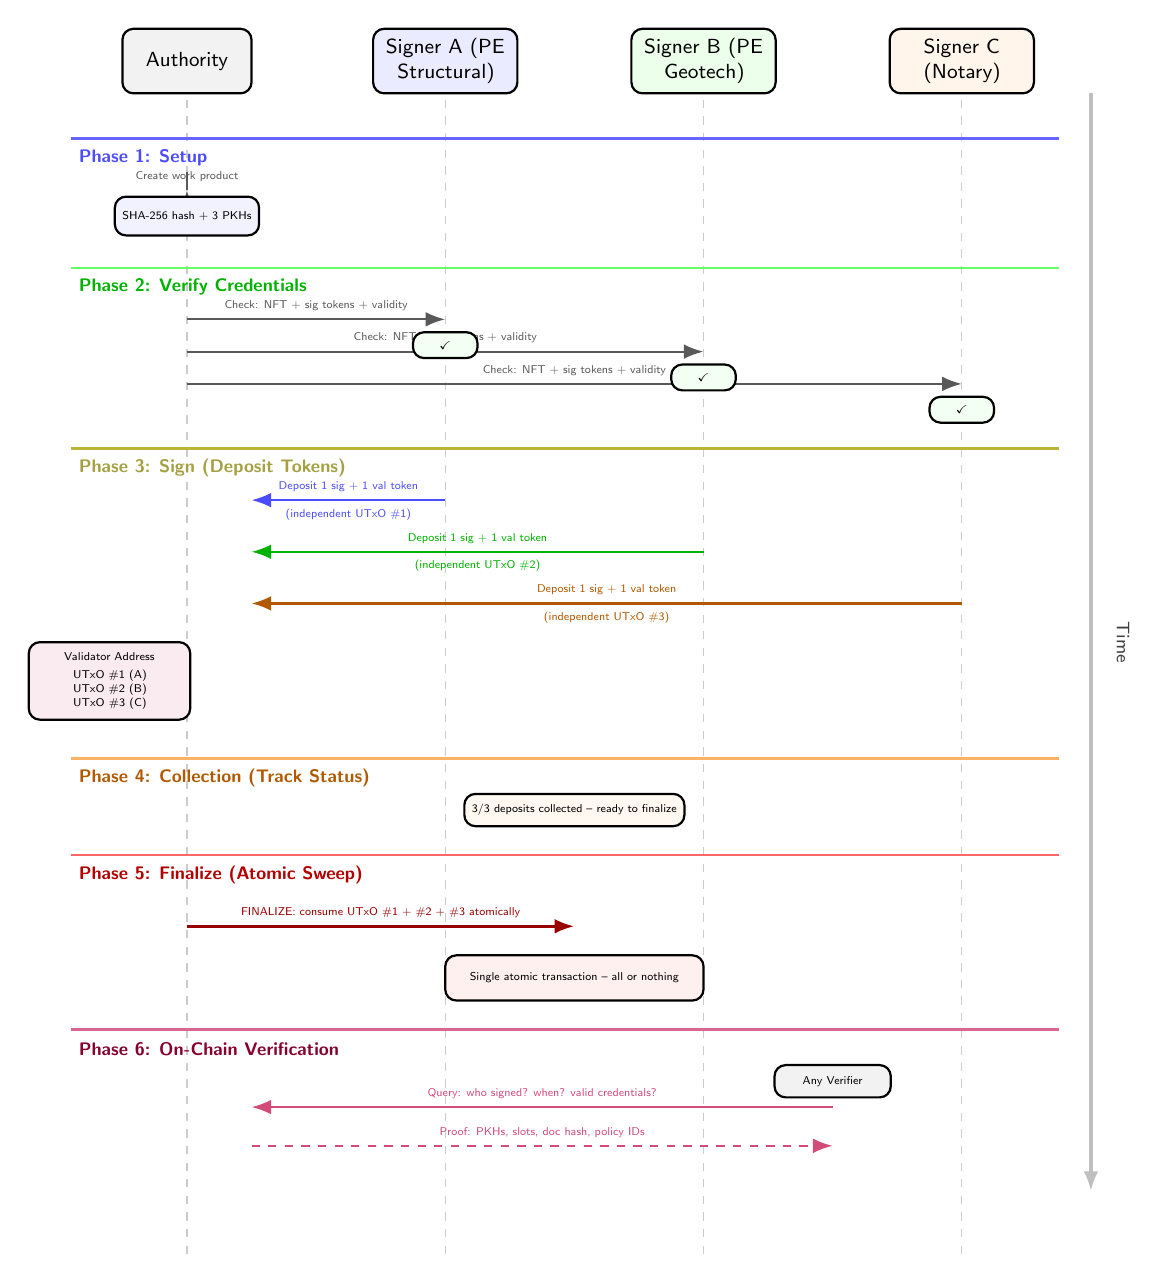
\begin{tikzpicture}[scale=0.82, every node/.style={transform shape}]
  % Actors
  \node[guidebox, fill=gray!10, minimum width=2cm] (authority) at (0,0)
    {Authority};
  \node[guidebox, fill=blue!8, minimum width=2cm, text width=2cm] (signerA) at (4,0)
    {Signer A (PE Structural)};
  \node[guidebox, fill=green!8, minimum width=2cm, text width=2cm] (signerB) at (8,0)
    {Signer B (PE Geotech)};
  \node[guidebox, fill=orange!8, minimum width=2cm, text width=2cm] (signerC) at (12,0)
    {Signer C (Notary)};

  % Lifelines
  \draw[dashed, gray!40] (0,-0.6) -- (0,-18.5);
  \draw[dashed, gray!40] (4,-0.6) -- (4,-18.5);
  \draw[dashed, gray!40] (8,-0.6) -- (8,-18.5);
  \draw[dashed, gray!40] (12,-0.6) -- (12,-18.5);

  % Phase 1: Setup
  \draw[thick, blue!60] (-1.8,-1.2) -- (13.5,-1.2);
  \node[guidelabel, anchor=west, font=\sffamily\footnotesize\bfseries,
    text=blue!70] at (-1.8,-1.5) {Phase 1: Setup};
  \draw[guidearrow] (0,-2) -- node[above, font=\sffamily\tiny]
    {Create work product} node[below, font=\sffamily\tiny]
    {(doc hash + signer list)} (0,-2);
  \node[guidebox, fill=blue!5, minimum width=2.2cm, minimum height=0.6cm,
    font=\sffamily\tiny, text width=2cm] at (0,-2.4) {SHA-256 hash + 3 PKHs};

  % Phase 2: Verify
  \draw[thick, green!60] (-1.8,-3.2) -- (13.5,-3.2);
  \node[guidelabel, anchor=west, font=\sffamily\footnotesize\bfseries,
    text=green!70!black] at (-1.8,-3.5) {Phase 2: Verify Credentials};
  \draw[guidearrow] (0,-4) -- node[above, font=\sffamily\tiny]
    {Check: NFT + sig tokens + validity} (4,-4);
  \draw[guidearrow] (0,-4.5) -- node[above, font=\sffamily\tiny]
    {Check: NFT + sig tokens + validity} (8,-4.5);
  \draw[guidearrow] (0,-5) -- node[above, font=\sffamily\tiny]
    {Check: NFT + sig tokens + validity} (12,-5);
  \node[guidebox, fill=green!5, minimum width=1cm, minimum height=0.4cm,
    font=\sffamily\tiny] at (4,-4.4) {\checkmark};
  \node[guidebox, fill=green!5, minimum width=1cm, minimum height=0.4cm,
    font=\sffamily\tiny] at (8,-4.9) {\checkmark};
  \node[guidebox, fill=green!5, minimum width=1cm, minimum height=0.4cm,
    font=\sffamily\tiny] at (12,-5.4) {\checkmark};

  % Phase 3: Sign
  \draw[thick, yellow!70!black] (-1.8,-6.0) -- (13.5,-6.0);
  \node[guidelabel, anchor=west, font=\sffamily\footnotesize\bfseries,
    text=yellow!60!black] at (-1.8,-6.3) {Phase 3: Sign (Deposit Tokens)};
  \draw[guidearrow, blue!70] (4,-6.8) -- node[above, font=\sffamily\tiny]
    {Deposit 1 sig + 1 val token} node[below, font=\sffamily\tiny]
    {(independent UTxO \#1)} (1,-6.8);
  \draw[guidearrow, green!70!black] (8,-7.6) -- node[above, font=\sffamily\tiny]
    {Deposit 1 sig + 1 val token} node[below, font=\sffamily\tiny]
    {(independent UTxO \#2)} (1,-7.6);
  \draw[guidearrow, orange!70!black] (12,-8.4) -- node[above, font=\sffamily\tiny]
    {Deposit 1 sig + 1 val token} node[below, font=\sffamily\tiny]
    {(independent UTxO \#3)} (1,-8.4);

  % Validator box
  \node[guidebox, fill=purple!8, minimum width=2.5cm, minimum height=1.2cm,
    font=\sffamily\tiny, text width=2.2cm] (valbox) at (-1.2,-9.6)
    {Validator Address\\[2pt]UTxO \#1 (A)\\UTxO \#2 (B)\\UTxO \#3 (C)};

  % Phase 4: Collect
  \draw[thick, orange!60] (-1.8,-10.8) -- (13.5,-10.8);
  \node[guidelabel, anchor=west, font=\sffamily\footnotesize\bfseries,
    text=orange!70!black] at (-1.8,-11.1) {Phase 4: Collection (Track Status)};
  \node[guidebox, fill=orange!5, minimum width=3cm, minimum height=0.5cm,
    font=\sffamily\tiny] at (6,-11.6) {3/3 deposits collected -- ready to finalize};

  % Phase 5: Finalize
  \draw[thick, red!60] (-1.8,-12.3) -- (13.5,-12.3);
  \node[guidelabel, anchor=west, font=\sffamily\footnotesize\bfseries,
    text=red!70!black] at (-1.8,-12.6) {Phase 5: Finalize (Atomic Sweep)};
  \draw[guidearrow, red!60!black, very thick] (0,-13.4) --
    node[above, font=\sffamily\tiny, text=red!60!black]
    {FINALIZE: consume UTxO \#1 + \#2 + \#3 atomically} (6,-13.4);
  \node[guidebox, fill=red!6, minimum width=4cm, minimum height=0.7cm,
    font=\sffamily\tiny] at (6,-14.2)
    {Single atomic transaction -- all or nothing};

  % Phase 6: Verify
  \draw[thick, purple!60] (-1.8,-15.0) -- (13.5,-15.0);
  \node[guidelabel, anchor=west, font=\sffamily\footnotesize\bfseries,
    text=purple!70!black] at (-1.8,-15.3) {Phase 6: On-Chain Verification};
  \node[guidebox, fill=gray!10, minimum width=1.8cm, minimum height=0.5cm,
    font=\sffamily\tiny] at (10,-15.8) {Any Verifier};
  \draw[guidearrow, purple!70] (10,-16.2) --
    node[above, font=\sffamily\tiny] {Query: who signed? when? valid credentials?}
    (1,-16.2);
  \draw[guidearrow, purple!70, dashed] (1,-16.8) --
    node[above, font=\sffamily\tiny] {Proof: PKHs, slots, doc hash, policy IDs}
    (10,-16.8);

  % Time arrow
  \draw[guidearrow, gray!50, very thick] (14,-0.5) -- (14,-17.5);
  \node[guidelabel, rotate=-90] at (14.5,-9) {Time};
\end{tikzpicture}
\caption{Complete six-phase multi-party signing sequence with three signers.
  Each signer creates an independent UTxO at the validator address (Phase~3),
  avoiding eUTxO concurrency conflicts.  The authority's finalize transaction
  (Phase~5) atomically consumes all deposits.}
\label{fig:six-phase-sequence}
\end{figure}


% ----------------------------------------------------------------------------
\section{The eUTxO Concurrency Solution}
\label{sec:eutxo-concurrency}

\subsection{Understanding the Problem}

Cardano uses the \textbf{extended UTxO (eUTxO) model}, which is
fundamentally different from Ethereum's account model.  In the account model,
a smart contract has a single ``account'' whose state is updated by
transactions.  Multiple transactions can modify the same account in the same
block (the EVM processes them sequentially within the block).  In the eUTxO
model, each UTxO is a discrete, one-time-use object: a transaction
\emph{consumes} one or more UTxOs and \emph{produces} new ones.  A UTxO can
be consumed exactly once---it is destroyed in the process.

This creates a concurrency challenge.  Suppose the system used a naive design
where all signers deposit into the \emph{same} UTxO at the validator address.
Signer~A sees UTxO~X (containing zero deposits) and builds a transaction that
consumes UTxO~X and produces UTxO~X$'$ (containing A's deposit).  Meanwhile,
Signer~B also sees UTxO~X and builds a transaction consuming it to produce
UTxO~X$''$ (containing B's deposit).  Both transactions reference UTxO~X as
an input.  But UTxO~X can only be consumed once.

When both transactions are submitted to the network, only one will succeed.
The other will fail with an error indicating that its input UTxO has already
been consumed.  This is the \textbf{eUTxO contention problem}: concurrent
transactions competing to spend the same UTxO cause all but one to fail.

In high-throughput DeFi applications on Cardano, this problem is well-known
and has motivated various batching and order-book designs.  For a credential
signing system, however, the problem is especially acute because signers are
\emph{expected} to act concurrently---telling three professionals ``please
sign one at a time and wait for on-chain confirmation between each'' is
operationally unacceptable.

\subsection{The Independent UTxO Solution}

The solution is elegant in its simplicity: \textbf{each signer creates their
own independent UTxO at the script address}.  There is no shared UTxO to
contend over.  Signer~A creates UTxO$_A$, Signer~B creates UTxO$_B$, and
Signer~C creates UTxO$_C$---all at the same validator address, but as
separate, non-conflicting UTxOs.  Since no two transactions reference the
same input, they can all succeed in the same block if submitted
simultaneously.

The authority then ``sweeps'' all per-signer UTxOs in a single finalization
transaction.  This finalize transaction has multiple inputs (one per signer
UTxO) and the authority's signature, and it is the only transaction that
needs to consume multiple UTxOs atomically.  Since only the authority submits
the finalize transaction, there is no concurrency conflict---only one party
is building this transaction.

\vspace{0.5cm}
\begin{figure}[H]
\centering
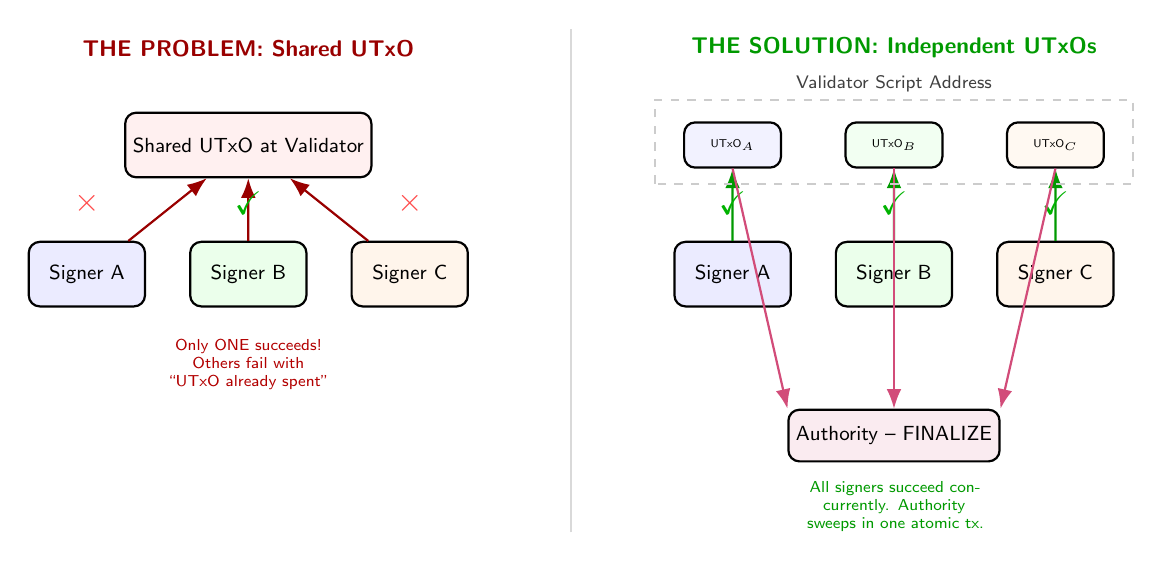
\begin{tikzpicture}[scale=0.82, every node/.style={transform shape}]
  % ---- LEFT SIDE: THE PROBLEM ----
  \node[font=\sffamily\bfseries, text=red!60!black] at (-4.5, 5.5)
    {THE PROBLEM: Shared UTxO};

  % Shared UTxO
  \node[guidebox, fill=red!6, minimum width=2.5cm, minimum height=1cm]
    (shared) at (-4.5, 4) {Shared UTxO at Validator};

  % Three signers trying to spend it
  \node[guidebox, fill=blue!8, minimum width=1.8cm] (sa) at (-7, 2) {Signer A};
  \node[guidebox, fill=green!8, minimum width=1.8cm] (sb) at (-4.5, 2) {Signer B};
  \node[guidebox, fill=orange!8, minimum width=1.8cm] (sc) at (-2, 2) {Signer C};

  \draw[guidearrow, red!60!black] (sa) -- (shared);
  \draw[guidearrow, red!60!black] (sb) -- (shared);
  \draw[guidearrow, red!60!black] (sc) -- (shared);

  % Conflict marker
  \node[font=\sffamily\scriptsize, text=red!70!black, text width=3cm,
    align=center] at (-4.5, 0.6)
    {Only ONE succeeds!\\Others fail with\\``UTxO already spent''};

  % X marks
  \node[font=\bfseries\Large, text=red!70] at (-7, 3.1) {$\times$};
  \node[font=\bfseries\Large, text=green!70!black] at (-4.5, 3.1) {\checkmark};
  \node[font=\bfseries\Large, text=red!70] at (-2, 3.1) {$\times$};

  % ---- RIGHT SIDE: THE SOLUTION ----
  \node[font=\sffamily\bfseries, text=green!60!black] at (5.5, 5.5)
    {THE SOLUTION: Independent UTxOs};

  % Three independent UTxOs
  \node[guidebox, fill=blue!8, minimum width=1.8cm] (sa2) at (3, 2)
    {Signer A};
  \node[guidebox, fill=green!8, minimum width=1.8cm] (sb2) at (5.5, 2)
    {Signer B};
  \node[guidebox, fill=orange!8, minimum width=1.8cm] (sc2) at (8, 2)
    {Signer C};

  % Independent UTxOs at validator
  \node[guidebox, fill=blue!5, minimum width=1.5cm, minimum height=0.7cm,
    font=\sffamily\tiny] (ua) at (3, 4) {UTxO$_A$};
  \node[guidebox, fill=green!5, minimum width=1.5cm, minimum height=0.7cm,
    font=\sffamily\tiny] (ub) at (5.5, 4) {UTxO$_B$};
  \node[guidebox, fill=orange!5, minimum width=1.5cm, minimum height=0.7cm,
    font=\sffamily\tiny] (uc) at (8, 4) {UTxO$_C$};

  \draw[guidearrow, green!60!black] (sa2) -- (ua);
  \draw[guidearrow, green!60!black] (sb2) -- (ub);
  \draw[guidearrow, green!60!black] (sc2) -- (uc);

  % All succeed
  \node[font=\bfseries\Large, text=green!70!black] at (3, 3.1) {\checkmark};
  \node[font=\bfseries\Large, text=green!70!black] at (5.5, 3.1) {\checkmark};
  \node[font=\bfseries\Large, text=green!70!black] at (8, 3.1) {\checkmark};

  % Authority sweep
  \node[guidebox, fill=purple!8, minimum width=3cm, minimum height=0.8cm]
    (auth) at (5.5, -0.5) {Authority -- FINALIZE};
  \draw[guidearrow, purple!70, thick] (ua.south) -- (auth.north west);
  \draw[guidearrow, purple!70, thick] (ub.south) -- (auth.north);
  \draw[guidearrow, purple!70, thick] (uc.south) -- (auth.north east);

  \node[font=\sffamily\scriptsize, text=green!60!black, text width=3.2cm,
    align=center] at (5.5, -1.6)
    {All signers succeed concurrently. Authority sweeps in one atomic tx.};

  % Validator address label
  \draw[dashed, gray!40, thick] (1.8, 3.4) rectangle (9.2, 4.7);
  \node[guidelabel, anchor=south] at (5.5, 4.7)
    {Validator Script Address};

  % Divider
  \draw[thick, gray!30] (0.5, -2) -- (0.5, 5.8);
\end{tikzpicture}
\caption{eUTxO concurrency: the shared-UTxO problem (left) versus the
  independent-UTxO solution (right).  When multiple signers target the same
  UTxO, only one transaction succeeds.  With independent UTxOs, all signers
  can deposit concurrently, and the authority sweeps all deposits in a single
  finalize transaction.}
\label{fig:eutxo-concurrency}
\end{figure}

\subsection{Why This Works in Cardano's Model}

The independent-UTxO pattern works because Cardano's eUTxO model treats each
UTxO as a separate object.  A validator script is identified by its script
hash, which determines the script address.  \emph{Any number of UTxOs} can
sit at the same script address, each with its own datum, its own tokens, and
its own spending conditions.  The validator script is invoked separately for
each UTxO being consumed, receiving the datum attached to \emph{that
specific UTxO} and the redeemer provided by the transaction.

This means the validator can enforce per-signer rules (``the datum's PKH
matches a required signer'') without needing to manage a shared state.
The ``global'' view---``have all required signers deposited?''---is checked
only in the finalize transaction, where the authority provides all UTxOs as
inputs and the script can verify completeness across the full input set.

This design pattern---per-user UTxOs at a shared script address, with a
privileged party performing the aggregation step---is a general solution
to eUTxO concurrency and is used in Cardano DEX order books, lending
protocols, and governance systems.  In the credential context, it maps
naturally to the real-world workflow: professionals act independently,
and an authority aggregates their actions into a final result.


% ----------------------------------------------------------------------------
\section{SignerDatum Structure}
\label{sec:signer-datum}

Each deposit UTxO at the validator address carries a \texttt{SignerDatum}---a
structured piece of data (a Plutus \texttt{PlutusData} type serialized as
CBOR) that creates an immutable record of the signing act.  The datum
contains five fields:

\begin{table}[H]
\centering
\caption{SignerDatum fields}
\label{tab:signer-datum}
\small
\begin{tabular}{@{}l l p{7cm}@{}}
\toprule
\textbf{Field} & \textbf{Type} & \textbf{Description} \\
\midrule
\texttt{signer\_pkh} & \texttt{PubKeyHash} (28 bytes) &
  The public key hash of the signer.  This is derived from the signer's
  Ed25519 verification key and serves as the on-chain identity binding.
  Combined with the transaction signature, it proves that the holder of
  the corresponding private key authorized this deposit. \\
\texttt{document\_hash} & \texttt{ByteString} (32 bytes) &
  The SHA-256 hash of the document being signed.  This binds the signature
  to a specific, unalterable document version.  Any party with the original
  document can recompute the hash and verify it matches. \\
\texttt{policy\_id} & \texttt{MintingPolicyHash} (28 bytes) &
  The policy ID under which the signer's credential tokens were minted.
  This allows verifiers to confirm which authority issued the signer's
  credentials, establishing provenance. \\
\texttt{validity\_expiry} & \texttt{POSIXTime} (slot number) &
  The expiry slot of the validity token deposited alongside this datum.
  Combined with \texttt{deposit\_slot}, this field proves that the signer's
  credentials were valid (not expired) at the time of signing. \\
\texttt{deposit\_slot} & \texttt{POSIXTime} (slot number) &
  The slot at which this deposit transaction was included in a block.
  This provides a precise timestamp of the signing act, anchored to
  Cardano's consensus-verified slot timeline. \\
\bottomrule
\end{tabular}
\end{table}

The combination of these five fields creates a self-contained proof of
credential-verified signing.  A verifier needs nothing beyond the Cardano
blockchain to confirm:  (1)~\texttt{signer\_pkh} identifies who signed;
(2)~\texttt{document\_hash} identifies what was signed;
(3)~\texttt{policy\_id} identifies which authority vouches for the signer;
(4)~\texttt{validity\_expiry} $>$ \texttt{deposit\_slot} proves the
credential was valid at signing time.

The datum is attached to the UTxO when it is created (Phase~3) and becomes
part of the blockchain's permanent record when the UTxO is consumed (Phase~5).
Because Cardano stores spent transaction data in the immutable ledger history,
the \texttt{SignerDatum} is preserved indefinitely---even after the UTxO
itself has been spent.  This is the mechanism by which the system provides
permanent, tamper-proof signing records.


% ============================================================================
% PART B: PRIVACY AND COMPLIANCE
% ============================================================================

\vspace{0.5cm}
\noindent\rule{\textwidth}{1.2pt}
\begin{center}
  {\Large\sffamily\bfseries Part B: Privacy and Compliance}
\end{center}
\noindent\rule{\textwidth}{1.2pt}
\vspace{0.3cm}


% ----------------------------------------------------------------------------
\section{The Privacy Architecture}
\label{sec:privacy-architecture}

A blockchain is, by design, a public, transparent, and immutable ledger.
Every transaction, every token transfer, every datum is visible to anyone
running a node or querying an explorer.  This transparency is precisely
what makes blockchain valuable for credential verification---but it creates
an immediate tension with data privacy requirements.  You cannot put a
person's name, license number, home address, and date of birth on a public
blockchain and simultaneously comply with data protection laws.

The system resolves this tension through a strict \textbf{architectural
separation} between on-chain and off-chain data.  The principle is simple
but rigorously applied: \emph{anything that touches the blockchain must be
incapable of identifying a natural person without access to a separate,
private mapping.}

\subsection{On-Chain Data (Public, Immutable)}

The following data elements exist on the Cardano blockchain and are visible
to any observer:

\begin{itemize}[leftmargin=*, nosep, itemsep=4pt]
  \item \textbf{Policy IDs.}  These are Blake2b-224 hashes of minting
    scripts.  A policy ID like \texttt{a1b2c3...f4e5} reveals nothing about
    the authority that created it unless the observer already knows the
    mapping between policy IDs and authorities.
  \item \textbf{Token asset names.}  Names like \texttt{LIC\_PE\_001} or
    \texttt{SIG\_TOKEN} are visible on-chain but contain no personal data.
    The naming convention uses role-based prefixes, not personal identifiers.
  \item \textbf{Transaction signatures (PKHs).}  Public key hashes are
    28-byte values derived from Ed25519 verification keys.  A PKH like
    \texttt{8a3f...c7d2} is a pseudonym---it identifies a \emph{key pair},
    not a \emph{person}.  Without the off-chain mapping, an observer cannot
    determine whose key it is.
  \item \textbf{CIP-25/68 metadata fields.}  The on-chain metadata attached
    to license NFTs includes credential type, jurisdiction code, issue date,
    status, and policy-specific fields.  These are designed to be
    \emph{functionally useful} (a verifier can confirm ``this is a PE
    license issued in California that is currently active'') without being
    \emph{personally identifying} (the metadata does not include the
    licensee's name or license number).
  \item \textbf{Slot timestamps.}  Cardano's slot numbers provide temporal
    ordering and can be converted to UTC timestamps.  These record
    \emph{when} events occurred but not \emph{who} was involved (beyond
    the pseudonymous PKH).
\end{itemize}

\subsection{Off-Chain Data (Private, Erasable)}

Personal data that connects blockchain pseudonyms to real-world identities
is stored exclusively in an off-chain database:

\begin{itemize}[leftmargin=*, nosep, itemsep=4pt]
  \item \textbf{Full names} of licensees, signers, and authority contacts
  \item \textbf{License numbers} as assigned by the issuing jurisdiction
  \item \textbf{Physical addresses} and contact information
  \item \textbf{Email addresses} and phone numbers
  \item \textbf{PKH-to-identity mappings} that link on-chain pseudonyms
    to real people
\end{itemize}

This data is stored in an \textbf{AES-256-GCM encrypted SQLite database}.
The encryption ensures that even if an attacker gains access to the database
file, the contents are unreadable without the encryption key.

\vspace{0.5cm}
\begin{figure}[H]
\centering
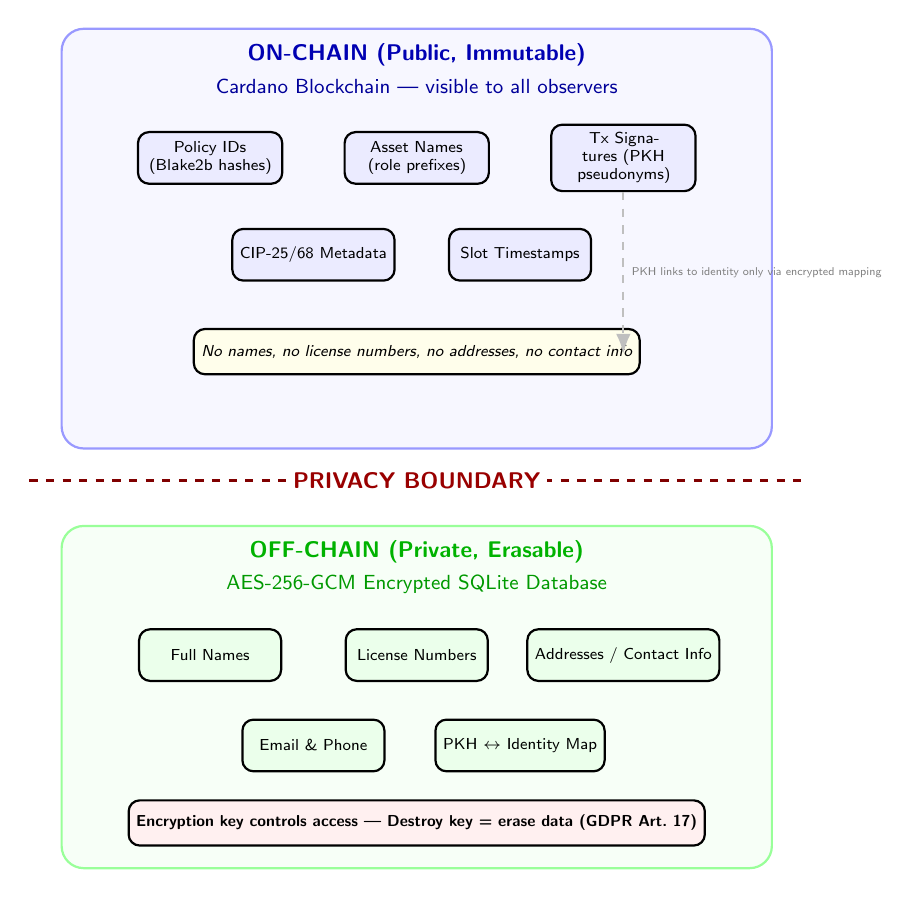
\begin{tikzpicture}[scale=0.82, every node/.style={transform shape}]
  % On-chain section
  \draw[thick, blue!40, rounded corners=8pt, fill=blue!3]
    (-5.5, 0) rectangle (5.5, 6.5);
  \node[font=\sffamily\bfseries, text=blue!70!black] at (0, 6.1)
    {ON-CHAIN (Public, Immutable)};
  \node[font=\sffamily\small, text=blue!60!black] at (0, 5.6)
    {Cardano Blockchain --- visible to all observers};

  \node[guidebox, fill=blue!8, minimum width=2.2cm, minimum height=0.8cm,
    font=\sffamily\scriptsize, text width=2cm] (pid) at (-3.2, 4.5) {Policy IDs (Blake2b hashes)};
  \node[guidebox, fill=blue!8, minimum width=2.2cm, minimum height=0.8cm,
    font=\sffamily\scriptsize, text width=2cm] (asset) at (0, 4.5) {Asset Names (role prefixes)};
  \node[guidebox, fill=blue!8, minimum width=2.2cm, minimum height=0.8cm,
    font=\sffamily\scriptsize, text width=2cm] (txsig) at (3.2, 4.5) {Tx Signatures (PKH pseudonyms)};

  \node[guidebox, fill=blue!8, minimum width=2.2cm, minimum height=0.8cm,
    font=\sffamily\scriptsize] (meta) at (-1.6, 3) {CIP-25/68 Metadata};
  \node[guidebox, fill=blue!8, minimum width=2.2cm, minimum height=0.8cm,
    font=\sffamily\scriptsize] (slots) at (1.6, 3) {Slot Timestamps};

  \node[guidebox, fill=yellow!8, minimum width=4cm, minimum height=0.7cm,
    font=\sffamily\scriptsize\itshape] at (0, 1.5)
    {No names, no license numbers, no addresses, no contact info};

  % Separator
  \draw[very thick, red!50!black, dashed] (-6, -0.5) -- (6, -0.5);
  \node[font=\sffamily\bfseries, text=red!60!black,
    fill=white, inner sep=3pt] at (0, -0.5)
    {PRIVACY BOUNDARY};

  % Off-chain section
  \draw[thick, green!40, rounded corners=8pt, fill=green!3]
    (-5.5, -6.5) rectangle (5.5, -1.2);
  \node[font=\sffamily\bfseries, text=green!70!black] at (0, -1.6)
    {OFF-CHAIN (Private, Erasable)};
  \node[font=\sffamily\small, text=green!60!black] at (0, -2.1)
    {AES-256-GCM Encrypted SQLite Database};

  \node[guidebox, fill=green!8, minimum width=2.2cm, minimum height=0.8cm,
    font=\sffamily\scriptsize] (names) at (-3.2, -3.2) {Full Names};
  \node[guidebox, fill=green!8, minimum width=2.2cm, minimum height=0.8cm,
    font=\sffamily\scriptsize] (licnum) at (0, -3.2) {License Numbers};
  \node[guidebox, fill=green!8, minimum width=2.2cm, minimum height=0.8cm,
    font=\sffamily\scriptsize] (addr) at (3.2, -3.2) {Addresses / Contact Info};

  \node[guidebox, fill=green!8, minimum width=2.2cm, minimum height=0.8cm,
    font=\sffamily\scriptsize] (email) at (-1.6, -4.6) {Email \& Phone};
  \node[guidebox, fill=green!8, minimum width=2.2cm, minimum height=0.8cm,
    font=\sffamily\scriptsize] (mapping) at (1.6, -4.6) {PKH $\leftrightarrow$ Identity Map};

  % Lock icon area
  \node[guidebox, fill=red!6, minimum width=4cm, minimum height=0.7cm,
    font=\sffamily\scriptsize\bfseries] at (0, -5.8)
    {Encryption key controls access --- Destroy key = erase data (GDPR Art.\ 17)};

  % Connection arrows
  \draw[guidearrow, dashed, gray!50] (txsig.south) -- ++(0,-2.5)
    node[midway, right, font=\sffamily\tiny, text=gray]
    {PKH links to identity only via encrypted mapping};
\end{tikzpicture}
\caption{Privacy architecture: strict separation between public on-chain data
  (policy IDs, asset names, PKHs, metadata, timestamps) and private off-chain
  data (names, license numbers, addresses, contact information).  The PKH-to-identity
  mapping exists only in the encrypted off-chain database.}
\label{fig:privacy-split}
\end{figure}


% ----------------------------------------------------------------------------
\section{AES-256-GCM Encryption}
\label{sec:aes256gcm}

The off-chain database and the authority's wallet keys at rest are protected
by \textbf{AES-256-GCM} encryption.  Understanding what this means requires
unpacking the acronym:

\textbf{AES} stands for \emph{Advanced Encryption Standard}, a symmetric-key
encryption algorithm adopted by NIST in 2001 (FIPS~197).  ``Symmetric-key''
means the same key is used for both encryption and decryption.  AES operates
on 128-bit blocks of data, transforming plaintext into ciphertext through a
series of substitution, permutation, and mixing operations.

\textbf{256} refers to the key length in bits.  A 256-bit key provides
$2^{256}$ possible key values---a number so large ($\approx 1.16 \times
10^{77}$) that brute-force enumeration is considered computationally
infeasible for the foreseeable future, including against quantum computers
using Grover's algorithm (which reduces the effective security to 128 bits,
still considered sufficient).

\textbf{GCM} stands for \emph{Galois/Counter Mode}, an authenticated
encryption mode that provides two guarantees simultaneously:

\begin{enumerate}[nosep]
  \item \textbf{Confidentiality.}  The ciphertext reveals nothing about the
    plaintext to anyone who does not possess the key.  GCM achieves this
    using CTR (Counter) mode, which turns AES into a stream cipher by
    encrypting sequential counter values and XOR-ing the result with the
    plaintext.
  \item \textbf{Integrity and Authentication.}  GCM produces an
    authentication tag (typically 128 bits) alongside the ciphertext.  This
    tag is computed using Galois field multiplication over the ciphertext
    blocks.  When decrypting, the recipient recomputes the tag and compares
    it with the stored tag.  If even a single bit of the ciphertext has been
    tampered with, the tags will not match, and the decryption is rejected.
\end{enumerate}

The combination of confidentiality and integrity is critical for the
credential system.  Without integrity protection, an attacker who gains
access to the encrypted database could modify ciphertext bytes (even
without knowing the key) and potentially cause the decrypted data to
contain corrupted-but-accepted values.  GCM prevents this: any modification
to the ciphertext is detected and rejected.

In the credential system, AES-256-GCM is used in two contexts:

\begin{itemize}[nosep]
  \item \textbf{Authority wallet keys at rest.}  The authority's Ed25519
    signing key is encrypted before being stored in the SQLite database.
    The encryption key is derived from a passphrase or stored in a separate
    key management system.  This ensures that database compromise alone
    does not expose the authority's signing capability.
  \item \textbf{Off-chain PII database.}  Personal data (names, license
    numbers, addresses) is encrypted at the field level or database level.
    Per-credential encryption keys enable granular erasure: destroying one
    key renders one person's data permanently inaccessible without affecting
    other records.
\end{itemize}


% ----------------------------------------------------------------------------
\section{GDPR and Crypto-Shredding}
\label{sec:gdpr-crypto-shredding}

\subsection{The GDPR Dilemma}

The General Data Protection Regulation (GDPR), enforced across the European
Union since May 2018, establishes a comprehensive framework for personal data
protection.  Article~17 is the provision most directly in tension with
blockchain technology:

\begin{quote}
\textit{``The data subject shall have the right to obtain from the controller
the erasure of personal data concerning him or her without undue delay, and
the controller shall have the obligation to erase personal data without
undue delay\ldots''}  --- GDPR Article 17(1)
\end{quote}

This is the \textbf{right to erasure}, commonly called the ``right to be
forgotten.''  It requires that upon request, a data controller must delete
all personal data associated with the requesting individual.

Blockchain, however, is \emph{immutable by design}.  Once a transaction is
confirmed and finalized, it cannot be altered or deleted.  This is not a
bug---it is the core value proposition.  Credential verification depends on
the guarantee that a licensing board's attestation, once published, cannot
be retroactively modified or erased.

The tension is stark: GDPR says ``delete it,'' and blockchain says ``it
cannot be deleted.''  The European Data Protection Board (EDPB) has made
clear in its April 2025 guidelines that technical impossibility is not an
acceptable excuse for non-compliance, with penalties reaching up to 20
million EUR or 4\% of global annual turnover, whichever is higher.

\subsection{The Solution: Crypto-Shredding}

The credential system resolves this dilemma through a technique called
\textbf{crypto-shredding} (also known as cryptographic erasure).  The
approach is architecturally simple but legally significant:

\begin{enumerate}[nosep]
  \item \textbf{Personal data is never stored on-chain.}  As described in
    Section~\ref{sec:privacy-architecture}, names, license numbers,
    addresses, and other personally identifiable information (PII) exist
    only in the encrypted off-chain database.
  \item \textbf{Each credential's PII is encrypted with a per-credential
    key.}  Rather than encrypting the entire database with a single key,
    the system uses individual encryption keys for each person's data.
    This enables selective erasure without affecting other records.
  \item \textbf{To ``erase'' data, destroy the encryption key.}  When a
    data subject exercises their Article~17 right, the system destroys the
    encryption key associated with their data.  The encrypted ciphertext
    remains in the database, but without the key, it is computationally
    indistinguishable from random noise.  The data is effectively and
    permanently erased.
  \item \textbf{On-chain hashes become meaningless.}  The on-chain data
    consists of cryptographic hashes (policy IDs, PKHs, asset names) and
    metadata that does not contain PII.  A PKH like \texttt{8a3f...c7d2}
    cannot be reversed to recover the original public key (hash functions
    are one-way), and even if it could, the public key does not reveal
    the person's identity without the destroyed off-chain mapping.
\end{enumerate}

This approach aligns with guidance from two regulatory bodies:

\begin{itemize}[nosep]
  \item \textbf{French CNIL (2018).}  The Commission Nationale de
    l'Informatique et des Libert\'{e}s published guidelines recognizing
    that storing only hashed or encrypted data on-chain, combined with
    off-chain key management and destruction capabilities, constitutes
    a GDPR-compliant architecture.
  \item \textbf{EDPB Framework (2025).}  The European Data Protection Board's
    updated guidelines acknowledge crypto-shredding as a valid technical
    measure for blockchain systems, provided that the on-chain data cannot
    be used to re-identify individuals after key destruction.
\end{itemize}

\vspace{0.5cm}
\begin{figure}[H]
\centering
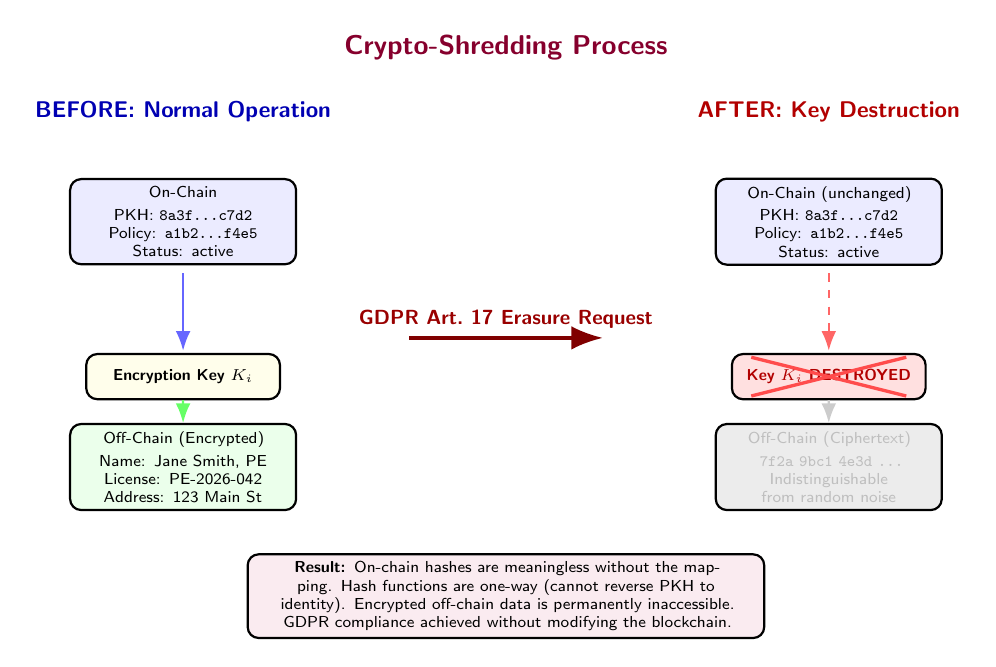
\begin{tikzpicture}[scale=0.82, every node/.style={transform shape}]
  % Title
  \node[font=\sffamily\bfseries\large, text=purple!70!black] at (0, 8.5)
    {Crypto-Shredding Process};

  % ---- BEFORE: Normal Operation ----
  \node[font=\sffamily\bfseries, text=blue!70!black] at (-5, 7.5)
    {BEFORE: Normal Operation};

  % On-chain
  \node[guidebox, fill=blue!8, minimum width=3.5cm, minimum height=1.2cm,
    font=\sffamily\scriptsize, text width=3cm] (onchain1) at (-5, 5.8)
    {On-Chain\\[2pt]PKH: \texttt{8a3f...c7d2}\\Policy: \texttt{a1b2...f4e5}\\Status: active};

  % Mapping arrow
  \draw[guidearrow, thick, blue!60] (-5, 5) -- (-5, 3.8);
  \node[guidebox, fill=yellow!8, minimum width=3cm, minimum height=0.7cm,
    font=\sffamily\scriptsize\bfseries] (key1) at (-5, 3.4)
    {Encryption Key $K_i$};

  % Off-chain
  \node[guidebox, fill=green!8, minimum width=3.5cm, minimum height=1.2cm,
    font=\sffamily\scriptsize, text width=3cm] (offchain1) at (-5, 2)
    {Off-Chain (Encrypted)\\[2pt]Name: Jane Smith, PE\\License: PE-2026-042\\Address: 123 Main St};

  \draw[guidearrow, thick, green!60] (key1) -- (offchain1.north);

  % ---- AFTER: Crypto-Shredding ----
  \node[font=\sffamily\bfseries, text=red!70!black] at (5, 7.5)
    {AFTER: Key Destruction};

  % On-chain (unchanged)
  \node[guidebox, fill=blue!8, minimum width=3.5cm, minimum height=1.2cm,
    font=\sffamily\scriptsize, text width=3cm] (onchain2) at (5, 5.8)
    {On-Chain (unchanged)\\[2pt]PKH: \texttt{8a3f...c7d2}\\Policy: \texttt{a1b2...f4e5}\\Status: active};

  % Key destroyed
  \draw[guidearrow, thick, red!60, dashed] (5, 5) -- (5, 3.8);
  \node[guidebox, fill=red!12, minimum width=3cm, minimum height=0.7cm,
    font=\sffamily\scriptsize\bfseries, text=red!70!black] (key2) at (5, 3.4)
    {Key $K_i$ DESTROYED};

  % Draw X over key
  \draw[very thick, red!70] (3.8, 3.1) -- (6.2, 3.7);
  \draw[very thick, red!70] (3.8, 3.7) -- (6.2, 3.1);

  % Off-chain (unreadable)
  \node[guidebox, fill=gray!15, minimum width=3.5cm, minimum height=1.2cm,
    font=\sffamily\scriptsize, text width=3cm, text=gray!50] (offchain2) at (5, 2)
    {Off-Chain (Ciphertext)\\[2pt]\texttt{7f2a 9bc1 4e3d ...}\\Indistinguishable\\from random noise};

  \draw[guidearrow, thick, gray!40, dashed] (key2) -- (offchain2.north);

  % Arrow from before to after
  \draw[-{Latex[length=4mm]}, very thick, red!50!black]
    (-1.5, 4) -- node[above, font=\sffamily\small\bfseries, text=red!60!black]
    {GDPR Art.\ 17 Erasure Request} (1.5, 4);

  % Result annotation
  \node[guidebox, fill=purple!8, minimum width=8cm, minimum height=1cm,
    font=\sffamily\scriptsize, text width=7.5cm] at (0, 0)
    {\textbf{Result:} On-chain hashes are meaningless without the mapping.
     Hash functions are one-way (cannot reverse PKH to identity).
     Encrypted off-chain data is permanently inaccessible.
     GDPR compliance achieved without modifying the blockchain.};
\end{tikzpicture}
\caption{Crypto-shredding process.  Left: during normal operation, the
  encryption key $K_i$ connects on-chain pseudonyms to off-chain personal
  data.  Right: after a GDPR erasure request, destroying $K_i$ renders the
  off-chain data permanently unreadable while on-chain hashes remain but
  become unlinkable to any natural person.}
\label{fig:crypto-shredding}
\end{figure}

\subsection{Why Hashes Cannot Be Reversed}

A common concern is: ``If the PKH is derived from a public key, can't
someone reverse the hash to recover the public key, and then use the public
key to identify the person?''  The answer is no, for two reasons:

First, Blake2b-224 (the hash function used for Cardano PKHs) is a
cryptographic hash function with preimage resistance.  Given a hash output
$h$, finding any input $x$ such that $\text{Blake2b-224}(x) = h$ requires
approximately $2^{224}$ operations---a number vastly exceeding the
computational capacity of all computers ever built.

Second, even if an attacker could somehow recover the public key from the
PKH, the public key is a 32-byte Ed25519 verification key.  This key does
not inherently contain any personal information.  The mapping from public
key to person exists only in the off-chain database---which has been
crypto-shredded.

The combination of one-way hash functions and off-chain key destruction
creates what privacy engineers call \textbf{unlinkability}: the on-chain
data points cannot be linked to a natural person after crypto-shredding,
satisfying the GDPR's erasure requirement in substance.


% ============================================================================
% PART C: LEGAL FRAMEWORK
% ============================================================================

\vspace{0.5cm}
\noindent\rule{\textwidth}{1.2pt}
\begin{center}
  {\Large\sffamily\bfseries Part C: Legal Framework}
\end{center}
\noindent\rule{\textwidth}{1.2pt}
\vspace{0.3cm}


% ----------------------------------------------------------------------------
\section{ESIGN Act (US Federal)}
\label{sec:esign}

The Electronic Signatures in Global and National Commerce Act (15~U.S.C.
\S\S~7001--7031), enacted in 2000, is the foundational US federal law
governing electronic signatures.  Its central provision is deceptively
simple: \emph{an electronic signature cannot be denied legal effect solely
because it is in electronic form}.  The Act is deliberately
technology-neutral---it does not prescribe \emph{how} an electronic
signature must be implemented, only that it must satisfy four requirements.

\subsection{Requirement 1: Intent to Sign}

The signer must demonstrate a deliberate intent to sign the document.  In
traditional e-signature tools, this is typically satisfied by clicking an
``I agree'' button.  In the credential system, intent is demonstrated by
the deliberate invocation of the \texttt{sign\_document()} function, which
requires the signer to:

\begin{itemize}[nosep]
  \item Identify the specific document (by hash) they are signing
  \item Decrypt their private signing key (requiring passphrase entry
    or hardware wallet interaction)
  \item Construct and submit an on-chain transaction that deposits tokens
    to the validator address
\end{itemize}

This multi-step process---far more deliberate than clicking a button---provides
strong evidence of intent.  A signer cannot accidentally deposit tokens to
a validator address; the process requires explicit, informed action at
multiple stages.

\subsection{Requirement 2: Consent to Conduct Business Electronically}

The signer must have consented to conducting business electronically.  The
credential system satisfies this through the onboarding process: when a
professional registers for the system and receives their wallet, credential
tokens, and access credentials, they explicitly accept terms of service that
include consent to electronic transactions.  This consent is recorded in the
off-chain database with a timestamp and is presented to the signer before
any wallet generation or token minting occurs.

\subsection{Requirement 3: Association of Signature with Record}

The electronic signature must be logically associated with the record being
signed.  The credential system achieves this through cryptographic binding
at three levels:

\begin{enumerate}[nosep]
  \item \textbf{SHA-256 hash binding.}  The \texttt{SignerDatum} includes
    the SHA-256 hash of the document, creating a mathematical link between
    the signature and the exact document version.
  \item \textbf{Transaction binding.}  The deposit transaction is signed
    with the signer's Ed25519 private key, cryptographically proving that
    the holder of that key authorized this specific transaction.
  \item \textbf{UTxO binding.}  The deposited tokens (signature token +
    validity token) are locked at the validator address with the
    \texttt{SignerDatum}, creating an inseparable on-chain association
    between the signer's identity, the document, and the signing act.
\end{enumerate}

This triple binding is significantly stronger than the ``email address
clicked a link'' association provided by most commercial e-signature tools.

\subsection{Requirement 4: Record Retention}

The signed record must be retained and reproducible.  The credential system
satisfies this through blockchain immutability: once the finalize transaction
is confirmed, the complete signing record---who signed, what they signed,
when they signed, and what credentials they held---is stored across
thousands of Cardano nodes worldwide.  The data cannot be altered, deleted,
or lost (short of a catastrophic failure of the entire Cardano network).
This level of retention surpasses any centralized storage system in both
durability and tamper-resistance.


% ----------------------------------------------------------------------------
\section{UETA (US State Law)}
\label{sec:ueta}

The Uniform Electronic Transactions Act (UETA) was drafted by the Uniform
Law Commission in 1999 and has been adopted by \textbf{49 states plus the
District of Columbia} (New York is the sole non-adopter, though it has its
own Electronic Signatures and Records Act).  UETA provides the state-level
legal foundation for electronic signatures, complementing the federal ESIGN
Act.

UETA's key contribution is Section~9, which establishes that an electronic
signature is ``attributable to a person'' if it can be shown by a
``preponderance of the evidence'' that the person performed the act.
Cardano's Ed25519 cryptography provides exceptionally strong attribution:
possessing the private key corresponding to a PKH is, in practice,
conclusive evidence of authorship.  The probability of forging an Ed25519
signature without the private key is approximately $2^{-128}$---effectively
zero.

\subsection{Blockchain-Specific State Amendments}

Nine states have gone beyond basic UETA adoption to enact
\textbf{blockchain-specific amendments} that explicitly recognize blockchain
signatures and smart contracts.  Two are particularly significant for the
credential system:

\textbf{Arizona HB 2417 (2017).}  Arizona was the first state to explicitly
recognize blockchain signatures.  A.R.S.~\S44-7061 provides that
``a signature that is secured through blockchain technology is considered
to be in an electronic form and to be an electronic signature'' and that
``a record or contract that is secured through blockchain technology is
considered to be in an electronic form and to be an electronic record.''
This statute directly validates the credential system's on-chain signing
mechanism: token deposits at a validator address, secured by Ed25519
cryptography on the Cardano blockchain, are electronic signatures under
Arizona law.

\textbf{Vermont 12 V.S.A. \S1913 (2016).}  Vermont's statute creates a
\textbf{rebuttable presumption of authenticity} for blockchain records.
Specifically, a ``digital record electronically registered in a blockchain''
is ``self-authenticating'' under the Vermont Rules of Evidence, provided that
the record is accompanied by a ``written declaration of a qualified person''
stating that the record is accurate.  This is an evidentiary advantage:
in court, the party introducing a blockchain-verified credential does not
bear the initial burden of proving its authenticity---the opposing party must
affirmatively rebut the presumption.  For the credential system, this means
that a finalized work product with on-chain signing records carries
automatic evidentiary weight in Vermont courts.

The remaining seven states with blockchain-specific provisions---Nevada,
Tennessee, South Dakota, Wyoming, Illinois, Colorado, and others---provide
varying degrees of explicit recognition for blockchain records and smart
contracts.  While the specific language differs, the trend is clear:
US state law is moving toward explicit statutory recognition of blockchain
as a valid medium for legally binding records and signatures.


% ----------------------------------------------------------------------------
\section{eIDAS 2.0 (European Union)}
\label{sec:eidas}

The European Union's electronic identification and trust services regulation,
known as eIDAS, is the most comprehensive legal framework for electronic
signatures globally.  The revised regulation, eIDAS~2.0 (Regulation (EU)
2024/1183), entered into force in 2024 and introduces provisions
specifically relevant to blockchain-based systems.

\subsection{Three Signature Tiers}

eIDAS~2.0 defines three tiers of electronic signatures, each with increasing
legal weight and technical requirements:

\textbf{Tier 1: Simple Electronic Signature (SES).}  The broadest category,
encompassing any ``data in electronic form which is attached to or logically
associated with other data in electronic form and which is used by the
signatory to sign.''  A typed name at the bottom of an email qualifies.
There are no technical requirements beyond basic logical association.  SES
signatures are admissible as evidence but carry no presumption of validity.

\textbf{Tier 2: Advanced Electronic Signature (AES).}  An AES must satisfy
four requirements defined in Article~26:

\begin{enumerate}[nosep]
  \item \textbf{Uniquely linked to the signatory.}  Each signer's Ed25519
    key pair is unique---no two signers share the same key.  The PKH
    derived from the verification key is a unique 28-byte identifier.
  \item \textbf{Capable of identifying the signatory.}  The PKH-to-identity
    mapping in the off-chain database links the cryptographic identity to
    a natural person.  The CIP-68 Reference Token's metadata provides
    additional identification context.
  \item \textbf{Created using data under the signatory's sole control.}
    The Ed25519 private key, stored encrypted in the signer's wallet
    (or in a hardware wallet via CIP-30), is under the signer's exclusive
    control.  No other party---including the authority---possesses the
    signer's private key.
  \item \textbf{Linked to the data signed in such a way that any
    subsequent change is detectable.}  The SHA-256 document hash in the
    \texttt{SignerDatum}, combined with the transaction signature, ensures
    that any modification to the signed document would produce a different
    hash, immediately detectable by any verifier.
\end{enumerate}

The credential system natively satisfies \textbf{all four AES requirements}
without requiring any modifications or additional infrastructure.  This is
a significant legal result: AES signatures carry a presumption of validity
across all EU member states and are admissible as evidence with enhanced
legal weight.

\textbf{Tier 3: Qualified Electronic Signature (QES).}  A QES is an AES
that is additionally:
\begin{itemize}[nosep]
  \item Created by a \textbf{Qualified Electronic Signature Creation
    Device (QSCD)}---a certified hardware device that protects the
    signing key
  \item Based on a \textbf{Qualified Certificate} issued by a
    \textbf{Qualified Trust Service Provider (QTSP)} that has been
    audited and approved by an EU member state's supervisory body
\end{itemize}

QES signatures have the \emph{legal equivalent of handwritten signatures}
across all EU member states.  The credential system does not natively
achieve QES status because it does not use a certified QSCD or a
QTSP-issued certificate.  However, a QTSP could integrate the credential
system's on-chain verification with its own qualified certificate
infrastructure to provide QES-level signatures.

\subsection{Qualified Electronic Ledger (Article 45l)}

eIDAS~2.0 introduces a new trust service category: the \textbf{Qualified
Electronic Ledger}.  Article~45l defines this as a distributed ledger
operated by a QTSP that provides ``proof of the existence and integrity of
electronic data recorded therein.''  This provision was specifically designed
to accommodate blockchain technology within the EU trust services framework.

For the credential system, Article~45l provides a clear pathway: if the
Cardano blockchain (or a specific Cardano-based service) obtains QTSP
status for ledger operation, then credentials recorded on it would carry
the full legal weight of a qualified trust service.  Cardano's formally
verified Ouroboros consensus protocol, with its published security proofs
in peer-reviewed venues, provides a strong technical foundation for such
qualification.

\vspace{0.5cm}
\begin{figure}[H]
\centering
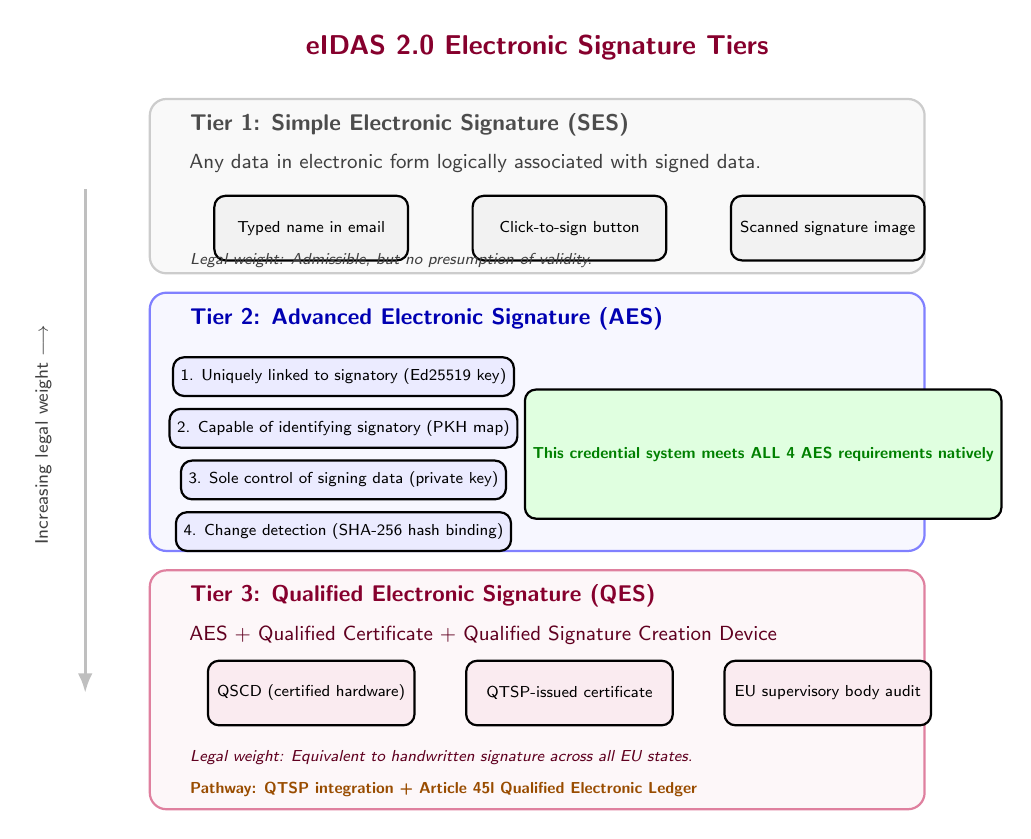
\begin{tikzpicture}[scale=0.82, every node/.style={transform shape}]
  % Title
  \node[font=\sffamily\bfseries\large, text=purple!70!black] at (0, 9)
    {eIDAS 2.0 Electronic Signature Tiers};

  % Tier 1: SES
  \draw[thick, gray!40, rounded corners=6pt, fill=gray!5]
    (-6, 5.5) rectangle (6, 8.2);
  \node[font=\sffamily\bfseries, text=gray!60!black, anchor=west]
    at (-5.5, 7.8) {Tier 1: Simple Electronic Signature (SES)};
  \node[font=\sffamily\small, text=gray!50!black, text width=10cm,
    anchor=west] at (-5.5, 7.2)
    {Any data in electronic form logically associated with signed data.};
  \node[guidebox, fill=gray!10, minimum width=3cm, font=\sffamily\scriptsize]
    at (-3.5, 6.2) {Typed name in email};
  \node[guidebox, fill=gray!10, minimum width=3cm, font=\sffamily\scriptsize]
    at (0.5, 6.2) {Click-to-sign button};
  \node[guidebox, fill=gray!10, minimum width=3cm, font=\sffamily\scriptsize]
    at (4.5, 6.2) {Scanned signature image};
  \node[font=\sffamily\scriptsize\itshape, text=gray!50!black, anchor=west]
    at (-5.5, 5.7) {Legal weight: Admissible, but no presumption of validity.};

  % Tier 2: AES
  \draw[thick, blue!50, rounded corners=6pt, fill=blue!3]
    (-6, 1.2) rectangle (6, 5.2);
  \node[font=\sffamily\bfseries, text=blue!70!black, anchor=west]
    at (-5.5, 4.8) {Tier 2: Advanced Electronic Signature (AES)};

  \node[guidebox, fill=blue!8, minimum width=4.8cm, minimum height=0.6cm,
    font=\sffamily\scriptsize] at (-3, 3.9)
    {1. Uniquely linked to signatory (Ed25519 key)};
  \node[guidebox, fill=blue!8, minimum width=4.8cm, minimum height=0.6cm,
    font=\sffamily\scriptsize] at (-3, 3.1)
    {2. Capable of identifying signatory (PKH map)};
  \node[guidebox, fill=blue!8, minimum width=4.8cm, minimum height=0.6cm,
    font=\sffamily\scriptsize] at (-3, 2.3)
    {3. Sole control of signing data (private key)};
  \node[guidebox, fill=blue!8, minimum width=4.8cm, minimum height=0.6cm,
    font=\sffamily\scriptsize] at (-3, 1.5)
    {4. Change detection (SHA-256 hash binding)};

  \node[guidebox, fill=green!12, minimum width=3.8cm, minimum height=2cm,
    font=\sffamily\scriptsize\bfseries, text=green!50!black] at (3.5, 2.7)
    {This credential system meets ALL 4 AES requirements natively};

  % Tier 3: QES
  \draw[thick, purple!50, rounded corners=6pt, fill=purple!3]
    (-6, -2.8) rectangle (6, 0.9);
  \node[font=\sffamily\bfseries, text=purple!70!black, anchor=west]
    at (-5.5, 0.5) {Tier 3: Qualified Electronic Signature (QES)};
  \node[font=\sffamily\small, text=purple!50!black, text width=10cm,
    anchor=west] at (-5.5, -0.1)
    {AES + Qualified Certificate + Qualified Signature Creation Device};

  \node[guidebox, fill=purple!8, minimum width=3.2cm, font=\sffamily\scriptsize]
    at (-3.5, -1) {QSCD (certified hardware)};
  \node[guidebox, fill=purple!8, minimum width=3.2cm, font=\sffamily\scriptsize]
    at (0.5, -1) {QTSP-issued certificate};
  \node[guidebox, fill=purple!8, minimum width=3.2cm, font=\sffamily\scriptsize]
    at (4.5, -1) {EU supervisory body audit};

  \node[font=\sffamily\scriptsize\itshape, text=purple!50!black, anchor=west]
    at (-5.5, -2)
    {Legal weight: Equivalent to handwritten signature across all EU states.};
  \node[font=\sffamily\scriptsize\bfseries, text=orange!60!black, anchor=west]
    at (-5.5, -2.5)
    {Pathway: QTSP integration + Article 45l Qualified Electronic Ledger};

  % Arrow showing progression
  \draw[guidearrow, very thick, gray!50] (-7, 6.8) -- (-7, 3.2)
    -- (-7, -1);
  \node[guidelabel, rotate=90, anchor=south] at (-7.4, 3)
    {Increasing legal weight $\longrightarrow$};
\end{tikzpicture}
\caption{eIDAS~2.0 electronic signature tiers.  The credential system
  natively meets all four Advanced Electronic Signature (AES) requirements.
  Qualified Electronic Signature (QES) status requires additional QTSP
  certification and hardware security modules, providing a clear upgrade
  pathway via Article~45l.}
\label{fig:eidas-tiers}
\end{figure}


% ----------------------------------------------------------------------------
\section{Putting It All Together: Compliance Summary}
\label{sec:compliance-summary}

The multi-party signing workflow, privacy architecture, and legal framework
are not independent concerns---they are three facets of a single design
problem.  The signing workflow must produce legally admissible records.
The privacy architecture must not undermine the evidentiary value of those
records.  The legal framework must be satisfied without compromising the
technical integrity of the system.

Table~\ref{tab:compliance-matrix} summarizes how each component of the system
maps to specific legal requirements across all three major frameworks.

\begin{table}[H]
\centering
\caption{Compliance matrix: system components mapped to legal requirements}
\label{tab:compliance-matrix}
\small
\begin{tabular}{@{}p{3cm} p{3.5cm} p{3.5cm} p{3.5cm}@{}}
\toprule
\textbf{System Component} & \textbf{ESIGN Act} & \textbf{UETA / State Law} & \textbf{eIDAS 2.0} \\
\midrule
Ed25519 key pair &
  Association (Req.~3) &
  Attribution (Sec.~9) &
  AES Reqs.~1, 3 \\
\texttt{sign\_document()} invocation &
  Intent (Req.~1) &
  Intent to sign &
  Signatory action \\
Onboarding consent &
  Consent (Req.~2) &
  Agreement to e-records &
  N/A \\
SHA-256 hash in datum &
  Association (Req.~3) &
  Record integrity &
  AES Req.~4 \\
Blockchain immutability &
  Retention (Req.~4) &
  Record preservation &
  Art.~45l ledger \\
CIP-68 credential status &
  N/A &
  Real-time verification &
  Trust service \\
Crypto-shredding &
  N/A &
  N/A &
  GDPR Art.~17 \\
PKH-to-identity mapping &
  N/A &
  N/A &
  AES Req.~2 \\
\bottomrule
\end{tabular}
\end{table}

The credential system achieves a rare balance: it provides stronger
cryptographic guarantees than traditional e-signature tools (SHA-256 hash
binding, Ed25519 signatures, immutable on-chain records), stronger credential
verification than any existing signing platform (real-time on-chain license
status), and GDPR compliance through architectural separation and
crypto-shredding---all while satisfying the requirements of three major
legal frameworks governing electronic signatures.

This compliance is not incidental; it is the result of architectural
decisions made at the system's foundation.  The separation of on-chain and
off-chain data, the use of PKHs as pseudonyms, the per-credential
encryption keys, and the independent-UTxO signing pattern were all
designed with legal requirements as first-class constraints alongside
technical requirements.

\section*{Chapter Summary}

\begin{itemize}[leftmargin=*, itemsep=4pt]
  \item Multi-party document signing uses a six-phase workflow: Setup,
    Verify, Sign, Collect, Finalize, Verify.  Each signer deposits tokens
    independently, and the authority finalizes atomically.
  \item The eUTxO concurrency problem---where multiple signers competing for
    the same UTxO causes all but one to fail---is solved by having each
    signer create an independent UTxO at the validator address.
  \item The \texttt{SignerDatum} structure records five fields (signer PKH,
    document hash, policy ID, validity expiry, deposit slot) that together
    prove who signed, what they signed, when, and with what credentials.
  \item Privacy is achieved through strict architectural separation: only
    pseudonymous hashes and policy IDs go on-chain; all personal data stays
    in an AES-256-GCM encrypted off-chain database.
  \item GDPR compliance is achieved through crypto-shredding: destroying
    per-credential encryption keys renders off-chain personal data
    permanently inaccessible while on-chain hashes remain meaningless
    without the mapping.
  \item The ESIGN Act requires intent, consent, association, and retention---all
    satisfied by the system's deliberate signing process, onboarding flow,
    hash binding, and blockchain immutability.
  \item UETA, adopted by 49 states plus DC, provides the state-level legal
    foundation; nine states have blockchain-specific amendments with Arizona
    and Vermont being the most significant.
  \item eIDAS~2.0 defines three signature tiers (SES, AES, QES).  The
    credential system natively meets all four AES requirements.  Article~45l
    provides a pathway to qualified trust service status through the new
    ``Qualified Electronic Ledger'' category.
\end{itemize}


% ============================================================================
% CHAPTER 7: Software & v4.0 Roadmap
% ============================================================================
% ============================================================================
% Chapter 7: The Software and the v4.0 Roadmap
% Study Guide — Cardano Credential Verification
% ============================================================================

\chapter{The Software and the v4.0 Roadmap}
\label{ch:software-roadmap}

This chapter is divided into three parts.  Part~A describes the
\texttt{cardano-license} Python package---its architecture, API surface,
database schema, and testing infrastructure.  Part~B presents the v4.0
roadmap: Aiken smart contracts, CIP-33 reference scripts, validity-token
consolidation, HSM key storage, and KERI/multi-sig governance.  Part~C
collects a comprehensive glossary of every technical term used throughout the
study guide.

% ── TikZ style definitions for this chapter ──────────────────────────────────
\tikzset{
  guidebox/.style={draw, rounded corners=4pt, thick, align=center,
    font=\sffamily\small, fill=white, minimum height=1cm},
  guidearrow/.style={-{Latex[length=2.5mm]}, thick, color=gray!70!black},
  guidelabel/.style={font=\sffamily\footnotesize, text=gray!50!black},
}


% ============================================================================
%  PART A — THE SOFTWARE
% ============================================================================

\vspace{0.5em}
\noindent\rule{\textwidth}{0.8pt}
\begin{center}
  {\Large\sffamily\bfseries Part A --- The Software}
\end{center}
\noindent\rule{\textwidth}{0.4pt}
\vspace{0.5em}


% ----------------------------------------------------------------------------
\section{Package Overview}
\label{sec:pkg-overview}

The \texttt{cardano-license} package is an open-source Python library
released under the MIT license.  As of this writing, the current release is
version~2.1.0.  The package provides a complete toolkit for professional
credential management on the Cardano blockchain, encompassing wallet
generation, license NFT minting, signature-token operations, validity
management, CIP-68 reference-token revocation, Plutus~V2 smart-contract
deployment, and dues enforcement.

Installation is straightforward via the Python Package Index:

\begin{lstlisting}[language=bash, caption={Installing cardano-license}]
pip install cardano-license
\end{lstlisting}

The package requires Python~3.10 or later and depends on four core
libraries.  \textbf{PyCardano} serves as the Cardano SDK, providing
HD~wallet generation, transaction building, Plutus~V2 script support, and
address derivation.  \textbf{Blockfrost} provides the chain-query API,
enabling the package to interact with the Cardano blockchain without running
a full node.  \textbf{aiosqlite} provides asynchronous SQLite database
access, allowing the package to maintain local state (wallets, licenses,
signatures, contracts) without blocking the event loop.
\textbf{cryptography} provides AES-256-GCM authenticated encryption for
wallet key files, using PBKDF2-HMAC-SHA256 key derivation with 100\,000
iterations.

\begin{table}[htbp]
\centering
\caption{Core dependencies of the \texttt{cardano-license} package.}
\label{tab:dependencies}
\begin{tabular}{@{}llp{6.5cm}@{}}
\toprule
\textbf{Library} & \textbf{Role} & \textbf{Usage} \\
\midrule
PyCardano        & Cardano SDK   & HD wallets, transaction building, Plutus~V2 scripts, CIP-1852 derivation \\
Blockfrost       & Chain API     & UTxO queries, transaction submission, balance lookups \\
aiosqlite        & Async DB      & Local persistence of wallets, licenses, signatures, contracts \\
cryptography     & Encryption    & AES-256-GCM key-file encryption with PBKDF2 derivation \\
\bottomrule
\end{tabular}
\end{table}

The package follows a layered design philosophy: all on-chain interactions
flow through PyCardano and Blockfrost, all local state is managed through
aiosqlite, and all key material is protected by the cryptography module.
This separation of concerns means that swapping the chain backend (e.g.,
from Blockfrost to Ogmios) or the database engine (e.g., from SQLite to
PostgreSQL) would require changes to only one layer.


% ----------------------------------------------------------------------------
\section{Architecture}
\label{sec:architecture}

The package is organized into four Python modules, each with a clearly
defined responsibility.  Figure~\ref{fig:module-diagram} illustrates the
dependency relationships between modules and external libraries.

\begin{figure}[htbp]
\centering
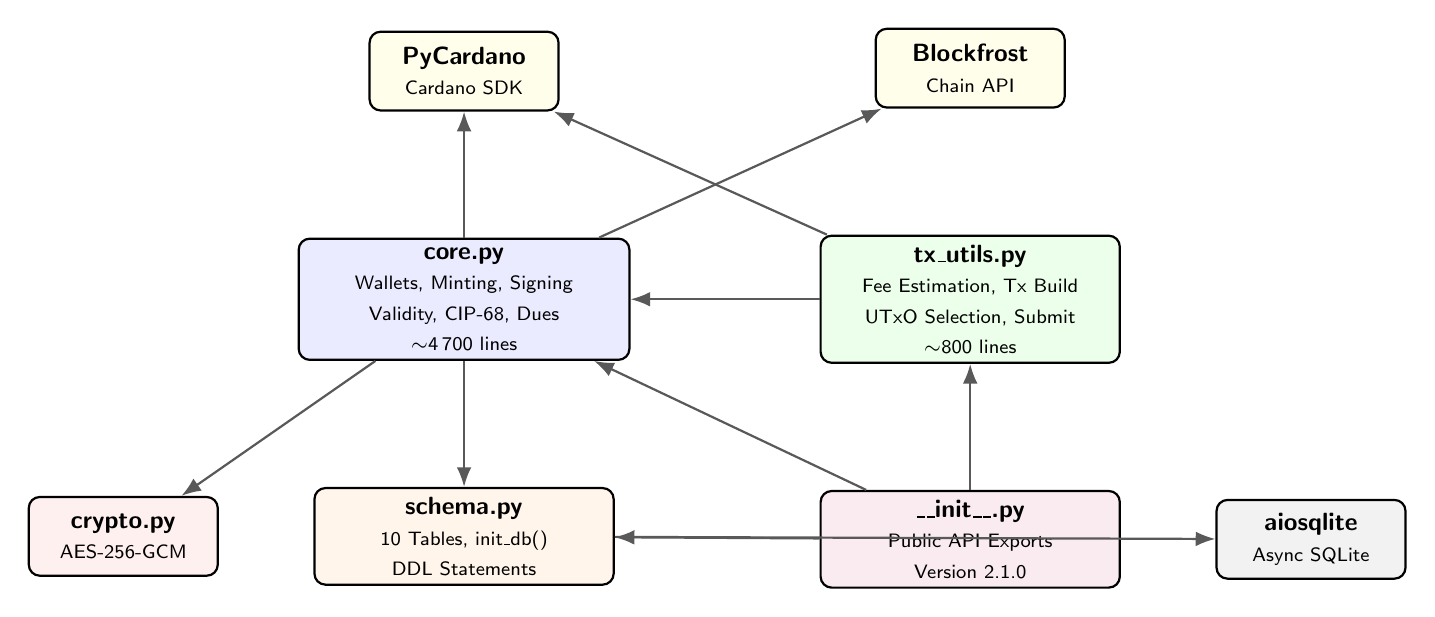
\begin{tikzpicture}[node distance=1.4cm and 2.2cm]
  % ── Internal modules ──
  \node[guidebox, fill=blue!8, minimum width=4.2cm]
    (core) {\textbf{core.py}\\{\scriptsize\textsf{Wallets, Minting, Signing}}\\{\scriptsize\textsf{Validity, CIP-68, Dues}}\\{\scriptsize\textsf{$\sim$4\,700 lines}}};

  \node[guidebox, fill=green!8, minimum width=3.8cm, right=2.4cm of core]
    (tx) {\textbf{tx\_utils.py}\\{\scriptsize\textsf{Fee Estimation, Tx Build}}\\{\scriptsize\textsf{UTxO Selection, Submit}}\\{\scriptsize\textsf{$\sim$800 lines}}};

  \node[guidebox, fill=orange!8, minimum width=3.8cm, below=1.6cm of core]
    (schema) {\textbf{schema.py}\\{\scriptsize\textsf{10 Tables, init\_db()}}\\{\scriptsize\textsf{DDL Statements}}};

  \node[guidebox, fill=purple!8, minimum width=3.8cm, below=1.6cm of tx]
    (init) {\textbf{\_\_init\_\_.py}\\{\scriptsize\textsf{Public API Exports}}\\{\scriptsize\textsf{Version 2.1.0}}};

  % ── External libraries ──
  \node[guidebox, fill=yellow!8, minimum width=2.4cm, above=1.6cm of core]
    (pycardano) {\textbf{PyCardano}\\{\scriptsize\textsf{Cardano SDK}}};

  \node[guidebox, fill=yellow!8, minimum width=2.4cm, above=1.6cm of tx]
    (blockfrost) {\textbf{Blockfrost}\\{\scriptsize\textsf{Chain API}}};

  \node[guidebox, fill=red!6, minimum width=2.4cm, left=1.2cm of schema]
    (crypto) {\textbf{crypto.py}\\{\scriptsize\textsf{AES-256-GCM}}};

  \node[guidebox, fill=gray!10, minimum width=2.4cm, right=1.2cm of init]
    (aiosqlite) {\textbf{aiosqlite}\\{\scriptsize\textsf{Async SQLite}}};

  % ── Arrows ──
  \draw[guidearrow] (core) -- (pycardano);
  \draw[guidearrow] (core) -- (blockfrost);
  \draw[guidearrow] (tx)   -- (pycardano);
  \draw[guidearrow] (tx)   -- (core);
  \draw[guidearrow] (core) -- (schema);
  \draw[guidearrow] (core) -- (crypto);
  \draw[guidearrow] (schema) -- (aiosqlite);
  \draw[guidearrow] (init) -- (core);
  \draw[guidearrow] (init) -- (tx);
  \draw[guidearrow] (init) -- (schema);
\end{tikzpicture}
\caption{Module dependency diagram for \texttt{cardano-license}.  Arrows
  point from the dependent module to the dependency.  Yellow boxes are
  external libraries; colored boxes are internal modules.}
\label{fig:module-diagram}
\end{figure}

\subsection{core.py --- The Main Module}

The \texttt{core.py} module is the heart of the package, weighing in at
approximately 4\,700~lines of Python.  It implements every domain operation
in the credential lifecycle: HD~wallet generation following the CIP-1852
derivation standard, authority-restricted minting-policy creation,
CIP-25--compliant license NFT minting, CIP-68 reference-token management
for authority-controlled revocation, signature-token minting and transfer,
validity-token minting and renewal, document signing with on-chain metadata,
multi-signer work-product coordination, Plutus~V2 signature-collection
validators with atomic finalization, and dues-enforcement contracts with
grace-period logic.

The module is organized into logical sections, each corresponding to a phase
of the credential lifecycle.  Wallet operations come first, followed by
chain-context helpers, minting-policy management, license NFT operations,
signature-token operations, validity-token operations, CIP-68 revocation,
document signing and verification, work-product management, Plutus~V2
validators, and dues enforcement.  All database-touching functions are
\texttt{async} and use \texttt{aiosqlite} for non-blocking I/O.

\subsection{tx\_utils.py --- Transaction Utilities}

The \texttt{tx\_utils.py} module contains approximately 800~lines of
transaction-building utilities that abstract away the lower-level details of
Cardano transaction construction.  Its primary exports include fee
estimation (\texttt{estimate\_fee}, \texttt{estimate\_fee\_from\_context}),
UTxO selection (\texttt{select\_utxos}), and high-level transaction builders
(\texttt{build\_mint\_tx}, \texttt{build\_transfer\_tx},
\texttt{build\_multisig\_tx}).  It also provides
\texttt{submit\_tx} for transaction submission and
\texttt{wait\_for\_confirmation} for polling until a transaction appears
on-chain.

The module defines two important data classes.  \texttt{TxResult} captures
the outcome of any transaction operation---hash, fee, input/output counts,
minted assets, confirmation status, and any error.  \texttt{UTxOSelection}
encapsulates the result of UTxO selection, including the selected inputs,
total value, and change amount.

\subsection{schema.py --- Database Schema}

The \texttt{schema.py} module defines the SQLite schema for the package's
local state.  It contains ten \texttt{CREATE TABLE IF NOT EXISTS} statements
and exposes a single public function, \texttt{init\_db()}, which ensures all
tables exist.  The ten tables are described in detail in
Section~\ref{sec:db-schema}.

\subsection{\_\_init\_\_.py --- Package Exports}

The \texttt{\_\_init\_\_.py} module re-exports the public API from
\texttt{core.py}, \texttt{tx\_utils.py}, and \texttt{schema.py}.  It also
defines the package version (\texttt{\_\_version\_\_ = "2.1.0"}) and the
\texttt{\_\_all\_\_} list, which enumerates every public symbol.  This
module serves as the single entry point for consumers:
\texttt{from cardano\_license import generate\_wallet, mint\_license\_nft}.


% ----------------------------------------------------------------------------
\section{Key API Functions}
\label{sec:api-functions}

This section presents the six most important functions in the
\texttt{cardano-license} API, with usage examples.  Every function is
\texttt{async} and must be called within an asyncio event loop.

\subsection{generate\_wallet}

The \texttt{generate\_wallet} function creates a new HD~wallet following the
CIP-1852 derivation standard.  It generates a 24-word BIP-39 mnemonic,
derives payment and stake key pairs using hardened derivation paths
(\texttt{m/1852'/1815'/0'/0/0} for payment, \texttt{m/1852'/1815'/0'/2/0}
for stake), constructs a base address that combines both keys, encrypts the
private keys with AES-256-GCM, saves them to disk, and records the wallet
metadata in the \texttt{blockchain\_wallets} table.

The function accepts a \texttt{wallet\_type} parameter that must be one of
\texttt{authority}, \texttt{licensee}, \texttt{signer}, or
\texttt{observer}.  This type determines the wallet's role in the credential
system and is enforced by a CHECK constraint in the database schema.

\begin{lstlisting}[language=Python,
  caption={Generating an authority wallet.}]
import asyncio
from cardano_license import generate_wallet

async def main():
    wallet = await generate_wallet(
        wallet_type="authority",
        label="state_board_of_engineers",
    )
    print(f"Address:  {wallet['address']}")
    print(f"Mnemonic: {wallet['mnemonic']}")
    # Mnemonic: 24-word BIP-39 phrase (store securely!)
    # Keys saved to ~/.cardano-license/wallets/

asyncio.run(main())
\end{lstlisting}

\subsection{mint\_license\_nft}

The \texttt{mint\_license\_nft} function mints a CIP-25--compliant license
NFT and sends it to a licensee's address.  Under the hood, it loads the
authority wallet's keys from encrypted storage, creates a
\texttt{ScriptPubkey} minting policy restricted to the authority's
verification key hash, builds CIP-25 metadata containing the license
fields, constructs and signs a minting transaction, submits it to the
network via Blockfrost, and records the mint in the
\texttt{blockchain\_licenses} table.

The function validates all required metadata fields before performing any
on-chain operation, failing fast with a \texttt{ValueError} if any field is
missing.  The minting policy ensures that only the authority's signing key
can authorize the creation (or destruction) of tokens under that policy.

\begin{lstlisting}[language=Python,
  caption={Minting a license NFT for a professional engineer.}]
import asyncio
from cardano_license import mint_license_nft

async def main():
    result = await mint_license_nft(
        authority_wallet_label="state_board_of_engineers",
        licensee_address="addr_test1qz...",
        license_metadata={
            "name": "PE License - Jane Smith",
            "license_type": "Professional Engineer",
            "license_number": "PE-2026-00142",
            "jurisdiction": "New York",
            "issued_date": "2026-01-15",
            "expiry_date": "2028-01-15",
            "holder_name": "Jane Smith",
        },
    )
    print(f"Policy ID:  {result['policy_id']}")
    print(f"Token Name: {result['token_name']}")
    print(f"Tx Hash:    {result['tx_hash']}")

asyncio.run(main())
\end{lstlisting}

\subsection{update\_license\_status}

The \texttt{update\_license\_status} function implements CIP-68
authority-controlled revocation.  In the CIP-68 model, the authority holds a
Reference Token (label~100) whose inline datum contains the license status.
To revoke a license, the authority updates this datum to
\texttt{status='revoked'}, requiring only the authority's signature and
\emph{zero interaction} with the licensee's wallet.

This is a critical design property: the licensee's User Token (label~222)
remains in their wallet, but any verifier who checks the Reference Token's
datum will see the revoked status.  The authority retains unilateral control
over credential status without needing to burn or recall tokens from the
licensee.

\begin{lstlisting}[language=Python,
  caption={Revoking a license via CIP-68 datum update.}]
import asyncio
from cardano_license import update_license_status

async def main():
    result = await update_license_status(
        license_id=42,
        new_status="revoked",
        authority_wallet_label="state_board_of_engineers",
    )
    print(f"Old status: {result['old_status']}")
    print(f"New status: {result['new_status']}")
    print(f"Tx Hash:    {result['tx_hash']}")

asyncio.run(main())
\end{lstlisting}

\subsection{sign\_document}

The \texttt{sign\_document} function records a professional's signature on a
document by transferring signature and validity tokens to a contract wallet
address.  The function builds a transaction that transfers one signature
token and one validity token to the specified contract address, attaches the
document's SHA-256 hash as transaction metadata (label~367), and records the
timestamp in the \texttt{blockchain\_signatures} table.

Each signer deposits tokens to an independent UTxO at the contract address,
avoiding the eUTxO concurrency bottleneck that would arise if all signers
tried to spend the same UTxO simultaneously.  This design enables true
parallel signing.

\begin{lstlisting}[language=Python,
  caption={Signing a document with credential tokens.}]
import asyncio
from cardano_license import sign_document

async def main():
    result = await sign_document(
        signer_wallet_label="jane_smith_pe",
        document_hash="a1b2c3d4e5f6...64-char-sha256-hex",
        contract_address="addr_test1qr...",
        license_ref=42,
    )
    print(f"Signature ID: {result['signature_id']}")
    print(f"Tx Hash:      {result['tx_hash']}")
    print(f"Timestamp:    {result['timestamp']}")

asyncio.run(main())
\end{lstlisting}

\subsection{verify\_signature}

The \texttt{verify\_signature} function checks whether a document has been
signed by querying the local signature records and verifying each signer's
validity-token status.  It returns a comprehensive result including the
verification status, a list of all signatures, the signature count, and
work-product information if the document is part of a multi-signer work
product.

The verification process cross-references the
\texttt{blockchain\_signatures} table against the
\texttt{blockchain\_validity\_tokens} table to ensure that each signer held
a valid (unexpired, unrevoked) validity token at the time of signing.

\begin{lstlisting}[language=Python,
  caption={Verifying a document's signatures.}]
import asyncio
from cardano_license import verify_signature

async def main():
    result = await verify_signature(
        contract_address="addr_test1qr...",
        document_hash="a1b2c3d4e5f6...64-char-sha256-hex",
    )
    print(f"Verified:         {result['is_verified']}")
    print(f"Signature count:  {result['signature_count']}")
    for sig in result["signatures"]:
        print(f"  Signer: {sig['signer_address']}")
        print(f"  Time:   {sig['timestamp']}")

asyncio.run(main())
\end{lstlisting}

\subsection{pay\_dues}

The \texttt{pay\_dues} function records a dues payment against a
dues-enforcement contract and renews the associated validity token.  It
validates the payment amount against the contract's
\texttt{annual\_dues\_lovelace} requirement, records the payment in the
\texttt{dues\_payments} table, and updates the validity expiry.

The dues-enforcement system links credential validity to ongoing financial
obligations.  If a licensee fails to pay annual dues within the grace
period, the authority can invoke the \texttt{RevokeValidityRedeemer} to
revoke the validity token on-chain, effectively disabling the credential.

\begin{lstlisting}[language=Python,
  caption={Paying annual dues to maintain credential validity.}]
import asyncio
from cardano_license import pay_dues

async def main():
    result = await pay_dues(
        contract_id=7,
        payer_address="addr_test1qz...",
        payment_lovelace=50_000_000,   # 50 ADA
        new_expiry="2027-03-01T00:00:00Z",
    )
    print(f"Payment ID:  {result['payment_id']}")
    print(f"New Expiry:  {result['new_expiry']}")

asyncio.run(main())
\end{lstlisting}


% ----------------------------------------------------------------------------
\section{Database Schema}
\label{sec:db-schema}

The \texttt{cardano-license} package maintains local state in a SQLite
database with ten tables.  This database is \emph{not} a replacement for the
blockchain---it serves as a local index and cache that enables fast queries
without hitting the Blockfrost API for every operation.  The on-chain state
remains the authoritative source of truth for all token ownership,
transaction finality, and datum values.

Table~\ref{tab:db-schema} summarizes all ten tables.  The
entity-relationship diagram in Figure~\ref{fig:er-diagram} shows the key
foreign-key relationships.

\begin{table}[htbp]
\centering
\caption{Database schema: all ten tables in \texttt{cardano-license}.}
\label{tab:db-schema}
\small
\begin{tabular}{@{}p{3.8cm}p{3.2cm}p{5.5cm}@{}}
\toprule
\textbf{Table} & \textbf{Key Columns} & \textbf{Purpose} \\
\midrule
\texttt{blockchain\_wallets}
  & id, wallet\_type, address, public\_key\_hash, network, label
  & Stores wallet metadata for all four roles (authority, licensee, signer, observer) \\
\addlinespace
\texttt{blockchain\_licenses}
  & id, token\_name, policy\_id, licensee\_address, authority\_address, status
  & Tracks minted license NFTs with metadata, status, and validity dates \\
\addlinespace
\texttt{blockchain\_reference\_tokens}
  & id, license\_id, policy\_id, user\_token\_name, ref\_token\_name, datum\_json, status
  & CIP-68 reference tokens with mutable datum for authority-controlled revocation \\
\addlinespace
\texttt{blockchain\_signature\_tokens}
  & id, policy\_id, token\_name, licensee\_address, quantity, status
  & Signature token inventory per licensee \\
\addlinespace
\texttt{blockchain\_validity\_tokens}
  & id, policy\_id, token\_name, licensee\_address, valid\_until, status
  & Time-bounded validity tokens linked to licenses \\
\addlinespace
\texttt{blockchain\_signatures}
  & id, document\_hash, signer\_address, signature\_tx\_hash, signature\_datum
  & Individual signature records with document hash and timestamp \\
\addlinespace
\texttt{blockchain\_work\_products}
  & id, title, wp\_address, document\_hash, required\_signers\_json, status
  & Multi-signer work products with signature collection tracking \\
\addlinespace
\texttt{blockchain\_minting\_policies}
  & policy\_id, authority\_address, policy\_cbor\_hex, script\_type
  & Minting policy registry (native script and Plutus~V2) \\
\addlinespace
\texttt{dues\_contracts}
  & id, authority\_address, license\_ref, annual\_dues\_lovelace, grace\_period\_slots, status
  & Dues-enforcement contracts linking credential validity to financial obligations \\
\addlinespace
\texttt{dues\_payments}
  & id, contract\_id, payer\_address, amount\_lovelace, new\_expiry, status
  & Payment records against dues contracts with confirmation tracking \\
\bottomrule
\end{tabular}
\end{table}

\begin{figure}[htbp]
\centering
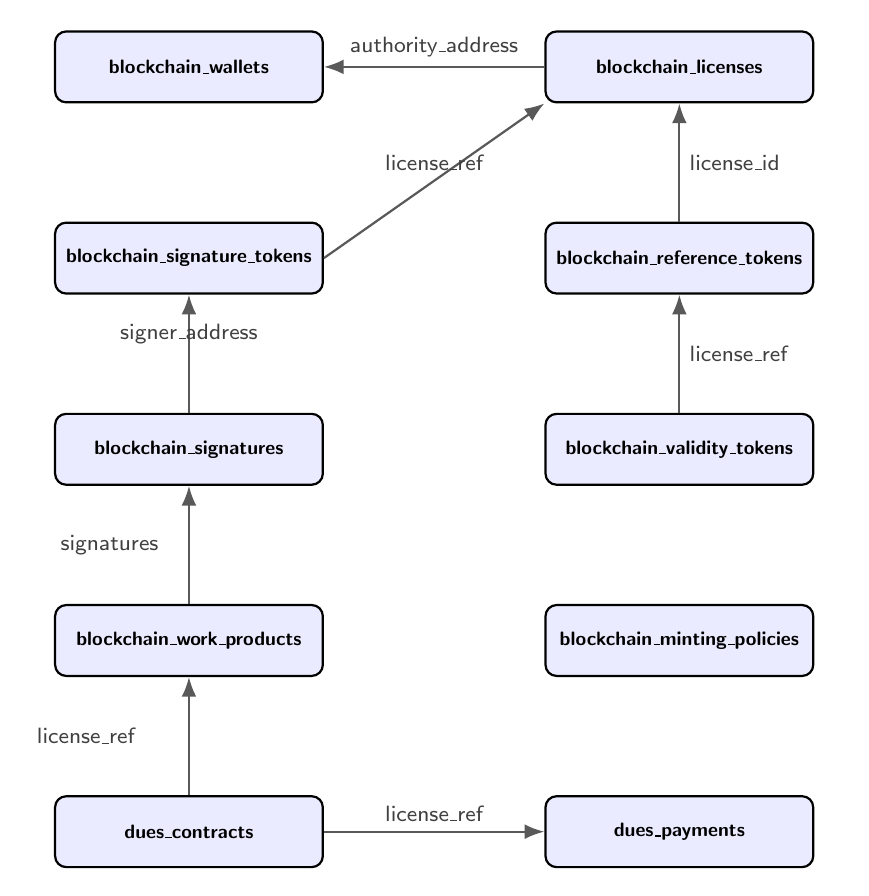
\begin{tikzpicture}[
  entity/.style={guidebox, fill=blue!8, minimum width=3.4cm, minimum height=0.9cm,
    font=\sffamily\scriptsize\bfseries},
  node distance=1.3cm and 2.6cm
]
  % ── Entities ──
  \node[entity] (wallets) {blockchain\_wallets};
  \node[entity, right=2.8cm of wallets] (licenses) {blockchain\_licenses};
  \node[entity, below=1.5cm of licenses] (reftokens) {blockchain\_reference\_tokens};
  \node[entity, below=1.5cm of wallets] (sigtokens) {blockchain\_signature\_tokens};
  \node[entity, below=1.5cm of reftokens] (valtokens) {blockchain\_validity\_tokens};
  \node[entity, below=1.5cm of sigtokens] (signatures) {blockchain\_signatures};
  \node[entity, below=1.5cm of signatures] (workproducts) {blockchain\_work\_products};
  \node[entity, below=1.5cm of valtokens] (policies) {blockchain\_minting\_policies};
  \node[entity, below=1.5cm of workproducts] (contracts) {dues\_contracts};
  \node[entity, below=1.5cm of policies] (payments) {dues\_payments};

  % ── Relationships ──
  \draw[guidearrow] (licenses) -- node[guidelabel, above] {authority\_address} (wallets);
  \draw[guidearrow] (reftokens) -- node[guidelabel, right, text width=1.8cm] {license\_id} (licenses);
  \draw[guidearrow] (sigtokens.east) -- node[guidelabel, above] {license\_ref} (licenses.south west);
  \draw[guidearrow] (valtokens) -- node[guidelabel, right, text width=1.8cm] {license\_ref} (reftokens);
  \draw[guidearrow] (signatures) -- node[guidelabel, above] {signer\_address} (sigtokens);
  \draw[guidearrow] (workproducts) -- node[guidelabel, left, text width=1.5cm] {signatures} (signatures);
  \draw[guidearrow] (contracts.east) -- node[guidelabel, above] {license\_ref} (payments.west);
  \draw[guidearrow] (contracts) -- node[guidelabel, left, text width=1.8cm] {license\_ref} (workproducts);
\end{tikzpicture}
\caption{Entity-relationship diagram for the \texttt{cardano-license} database.
  Arrows indicate referential relationships between tables.}
\label{fig:er-diagram}
\end{figure}

The schema enforces data integrity through CHECK constraints on enumerated
columns.  For example, the \texttt{blockchain\_wallets.wallet\_type} column
is constrained to \texttt{('authority', 'licensee', 'signer', 'observer')},
and the \texttt{blockchain\_licenses.status} column is constrained to
\texttt{('pending', 'active', 'revoked', 'expired', 'burned')}.  These
constraints prevent invalid state transitions at the database level,
providing a safety net independent of application-level validation.


% ----------------------------------------------------------------------------
\section{Configuration}
\label{sec:configuration}

The \texttt{cardano-license} package is configured entirely through
environment variables, following the twelve-factor app methodology.  This
design enables the same codebase to target mainnet, preprod, or preview
networks without code changes.

\begin{table}[htbp]
\centering
\caption{Environment variables for \texttt{cardano-license} configuration.}
\label{tab:env-vars}
\begin{tabular}{@{}p{4.6cm}p{2.8cm}p{5cm}@{}}
\toprule
\textbf{Variable} & \textbf{Default} & \textbf{Purpose} \\
\midrule
\texttt{CARDANO\_NETWORK}
  & \texttt{testnet}
  & Target network: \texttt{mainnet}, \texttt{testnet} (preprod), or \texttt{preview} \\
\addlinespace
\texttt{BLOCKFROST\_PROJECT\_ID}
  & (empty)
  & Blockfrost API key for chain queries and transaction submission \\
\addlinespace
\texttt{CARDANO\_LICENSE\_PASSWORD}
  & (empty)
  & Password for AES-256-GCM wallet key encryption; if empty, prompts interactively \\
\addlinespace
\texttt{CARDANO\_LICENSE\_DIR}
  & \texttt{\textasciitilde/.cardano-license}
  & Base directory for wallets, policies, and database \\
\addlinespace
\texttt{CARDANO\_LICENSE\_DB}
  & \texttt{<DIR>/license.db}
  & SQLite database file path \\
\bottomrule
\end{tabular}
\end{table}

The configuration module (\texttt{config.py}) automatically creates the
required directory structure on import: the base directory, the
\texttt{wallets/} subdirectory for encrypted key files, and the
\texttt{policies/} subdirectory for serialized minting-policy scripts.  This
means that a fresh installation requires no manual setup beyond setting the
environment variables.

For production deployments, the \texttt{CARDANO\_NETWORK} variable should be
set to \texttt{mainnet} and the \texttt{BLOCKFROST\_PROJECT\_ID} should
contain a mainnet API key obtained from the Blockfrost dashboard.  For
development and testing, the default \texttt{testnet} setting targets the
Cardano preprod network, where test ADA is freely available from faucets.


% ----------------------------------------------------------------------------
\section{Testing}
\label{sec:testing}

The \texttt{cardano-license} package includes a comprehensive test suite
with 660~passing tests.  The tests are organized into four test modules
covering the full spectrum of package functionality.

\texttt{test\_license.py} covers wallet management (generation, key
encryption/decryption, label lookup), license NFT operations (minting,
metadata validation, status queries), CIP-68 reference-token management
(store, update, revocation), signature-token operations (mint, balance,
transfer), validity-token operations (mint, check, renew, revoke), document
signing and verification, work-product lifecycle (create, sign, finalize),
and authority registration.

\texttt{test\_contracts.py} covers Plutus~V2 smart-contract operations:
signature-collection validator construction, datum and redeemer
serialization, dues-enforcement contract deployment, payment validation, and
grace-period logic.

\texttt{test\_tx\_utils.py} covers transaction-building utilities: fee
estimation, UTxO selection, mint/transfer/multisig transaction construction,
submission, and confirmation polling.

\texttt{test\_testnet.py} contains integration tests designed to run against
the Cardano preprod testnet with a live Blockfrost connection.  These tests
are marked with \texttt{@pytest.mark.testnet} and are skipped by default in
CI environments where testnet access is unavailable.

The test suite uses \texttt{pytest} with the \texttt{pytest-asyncio} plugin
for async test support.  All database-touching tests use isolated temporary
databases to prevent cross-test contamination.  Running the full suite
requires only:

\begin{lstlisting}[language=bash, caption={Running the test suite.}]
pytest tests/ -v
# 660 passed in ~45s (excluding testnet tests)
\end{lstlisting}


% ============================================================================
%  PART B — THE v4.0 ROADMAP
% ============================================================================

\vspace{1em}
\noindent\rule{\textwidth}{0.8pt}
\begin{center}
  {\Large\sffamily\bfseries Part B --- The v4.0 Roadmap}
\end{center}
\noindent\rule{\textwidth}{0.4pt}
\vspace{0.5em}


% ----------------------------------------------------------------------------
\section{Aiken Smart Contracts}
\label{sec:aiken}

The current implementation uses Plutus~V2 validators written as PyCardano
\texttt{PlutusV2Script} objects with serialized CBOR bytecode.  While
functional, this approach inherits the well-known limitations of the
PlutusTx/Haskell compilation pipeline: large compiled UPLC (Untyped Plutus
Lambda Calculus) output, high CPU and memory execution-unit (exUnit)
consumption, and a steep learning curve for developers unfamiliar with
Haskell.

Aiken is a modern smart-contract language designed specifically for Cardano.
It uses a Rust-like syntax that is far more accessible to the broader
developer community while maintaining the same security guarantees as
Haskell-compiled Plutus scripts.  The Aiken compiler produces significantly
smaller UPLC bytecode---often 5--10$\times$ smaller than equivalent PlutusTx
output---which directly translates to lower exUnit consumption and lower
transaction fees.

The v4.0 roadmap calls for rewriting all three of the credential system's
validators in Aiken: the signature-collection validator (which manages
multi-signer deposits, finalization sweeps, and reclaim operations), the
dues-enforcement validator (which links credential validity to payment
obligations), and the planned validity-consolidation validator (described in
Section~\ref{sec:validity-consolidation}).

The benefits of the Aiken migration are fourfold.  First, the compiled
script sizes will shrink dramatically, reducing the on-chain footprint.
Second, the smaller scripts consume fewer exUnits, lowering per-transaction
costs.  Third, the Rust-like syntax lowers the barrier to community
contributions and third-party auditing.  Fourth, the Aiken toolchain
includes built-in testing and property-based fuzzing, improving validator
correctness assurance.

\begin{figure}[htbp]
\centering
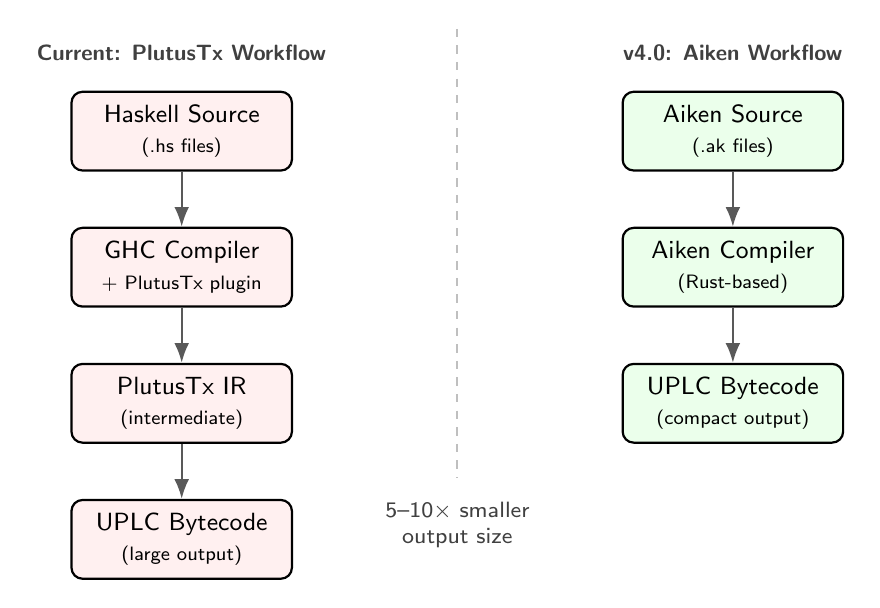
\begin{tikzpicture}[node distance=0.9cm and 1.2cm]
  % ── PlutusTx workflow (left) ──
  \node[guidelabel] at (-3.5, 3.2) {\textbf{Current: PlutusTx Workflow}};

  \node[guidebox, fill=red!6, minimum width=2.8cm] (haskell)
    at (-3.5, 2.2) {Haskell Source\\{\scriptsize\textsf{(.hs files)}}};
  \node[guidebox, fill=red!6, minimum width=2.8cm, below=0.7cm of haskell]
    (ghc) {GHC Compiler\\{\scriptsize\textsf{+ PlutusTx plugin}}};
  \node[guidebox, fill=red!6, minimum width=2.8cm, below=0.7cm of ghc]
    (plutustx) {PlutusTx IR\\{\scriptsize\textsf{(intermediate)}}};
  \node[guidebox, fill=red!6, minimum width=2.8cm, below=0.7cm of plutustx]
    (uplc1) {UPLC Bytecode\\{\scriptsize\textsf{(large output)}}};

  \draw[guidearrow] (haskell) -- (ghc);
  \draw[guidearrow] (ghc) -- (plutustx);
  \draw[guidearrow] (plutustx) -- (uplc1);

  % ── Aiken workflow (right) ──
  \node[guidelabel] at (3.5, 3.2) {\textbf{v4.0: Aiken Workflow}};

  \node[guidebox, fill=green!8, minimum width=2.8cm] (aiken)
    at (3.5, 2.2) {Aiken Source\\{\scriptsize\textsf{(.ak files)}}};
  \node[guidebox, fill=green!8, minimum width=2.8cm, below=0.7cm of aiken]
    (aikencc) {Aiken Compiler\\{\scriptsize\textsf{(Rust-based)}}};
  \node[guidebox, fill=green!8, minimum width=2.8cm, below=0.7cm of aikencc]
    (uplc2) {UPLC Bytecode\\{\scriptsize\textsf{(compact output)}}};

  \draw[guidearrow] (aiken) -- (aikencc);
  \draw[guidearrow] (aikencc) -- (uplc2);

  % ── Comparison annotation ──
  \draw[dashed, thick, gray!50] (0, 3.5) -- (0, -2.2);
  \node[guidelabel, text width=2.5cm, align=center] at (0, -2.8)
    {5--10$\times$ smaller\\output size};
\end{tikzpicture}
\caption{Compilation pipeline comparison: PlutusTx (left) requires three
  stages through the GHC/Haskell toolchain, producing large UPLC.  Aiken
  (right) compiles directly to compact UPLC in a single step.}
\label{fig:aiken-comparison}
\end{figure}


% ----------------------------------------------------------------------------
\section{CIP-33 Reference Scripts}
\label{sec:cip33}

In the current architecture, every transaction that invokes a Plutus
validator must attach the full compiled script bytecode.  For the
signature-collection validator, this adds several kilobytes to each signing
transaction.  For the dues-enforcement validator, it adds similar overhead
to every payment transaction.  This per-transaction overhead increases both
transaction size and fees.

CIP-33 (Reference Scripts) solves this problem by allowing validators to be
deployed to the blockchain \emph{once} as reference scripts.  The deploying
transaction creates a UTxO that carries the compiled script in its output.
Every subsequent transaction that needs to invoke that validator simply
references the UTxO containing the script, rather than attaching the full
bytecode.

The impact on transaction economics is substantial.  A typical
signature-deposit transaction currently weighs approximately 8--12~KB due to
the attached validator script.  With CIP-33 reference scripts, the same
transaction would weigh only 400--800~bytes---the script reference adds just
a 32-byte transaction hash and a UTxO index.  This reduction translates
directly to lower fees: roughly 80--90\% savings on script-bearing
transactions.

The v4.0 implementation plan is straightforward.  First, deploy each
validator (signature collection, dues enforcement, validity consolidation)
as a reference script in a dedicated UTxO.  Second, update the transaction
builders in \texttt{tx\_utils.py} to reference the script UTxO instead of
attaching the full bytecode.  Third, store the reference-script UTxO
identifiers in the \texttt{blockchain\_minting\_policies} table for
retrieval during transaction construction.

\begin{figure}[htbp]
\centering
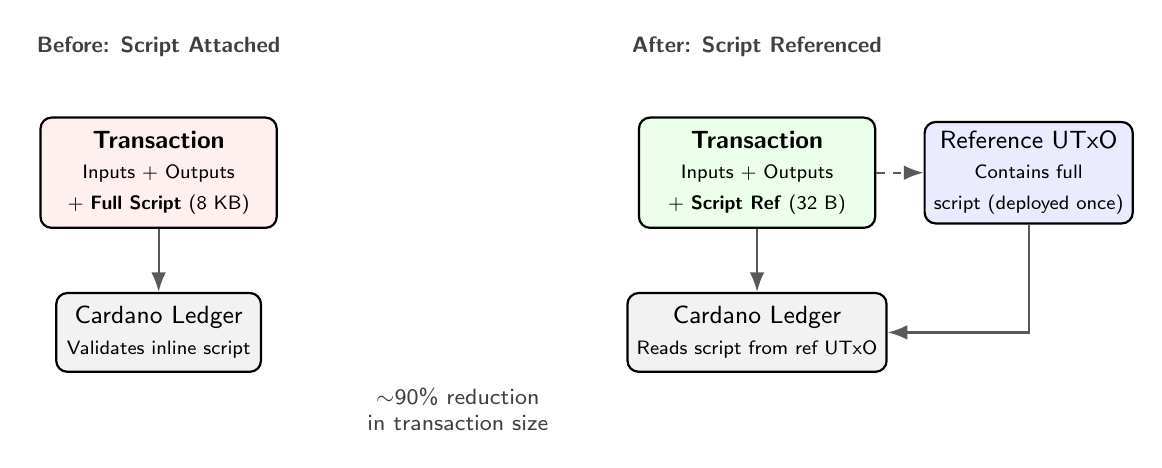
\begin{tikzpicture}[node distance=1cm and 1.5cm]
  % ── Before: Script Attached ──
  \node[guidelabel] at (-3.8, 2.8) {\textbf{Before: Script Attached}};

  \node[guidebox, fill=red!6, minimum width=3cm, minimum height=1.4cm]
    (txbefore) at (-3.8, 1.2)
    {\textbf{Transaction}\\{\scriptsize\textsf{Inputs + Outputs}}\\
     {\scriptsize\textsf{+ \textbf{Full Script} (8 KB)}}};

  \node[guidebox, fill=gray!10, minimum width=2.6cm, below=0.8cm of txbefore]
    (chain1) {Cardano Ledger\\{\scriptsize\textsf{Validates inline script}}};

  \draw[guidearrow] (txbefore) -- (chain1);

  % ── After: Script Referenced ──
  \node[guidelabel] at (3.8, 2.8) {\textbf{After: Script Referenced}};

  \node[guidebox, fill=green!8, minimum width=3cm, minimum height=1.4cm]
    (txafter) at (3.8, 1.2)
    {\textbf{Transaction}\\{\scriptsize\textsf{Inputs + Outputs}}\\
     {\scriptsize\textsf{+ \textbf{Script Ref} (32 B)}}};

  \node[guidebox, fill=blue!8, minimum width=2.6cm, right=0.6cm of txafter]
    (refutxo) {Reference UTxO\\{\scriptsize\textsf{Contains full}}\\
     {\scriptsize\textsf{script (deployed once)}}};

  \node[guidebox, fill=gray!10, minimum width=2.6cm, below=0.8cm of txafter]
    (chain2) {Cardano Ledger\\{\scriptsize\textsf{Reads script from ref UTxO}}};

  \draw[guidearrow] (txafter) -- (chain2);
  \draw[guidearrow, dashed] (txafter) -- (refutxo);
  \draw[guidearrow] (refutxo) |- (chain2);

  % ── Savings annotation ──
  \node[guidelabel, text width=3cm, align=center] at (0, -1.8)
    {$\sim$90\% reduction\\in transaction size};
\end{tikzpicture}
\caption{CIP-33 Reference Scripts: before (left), each transaction carries
  the full validator bytecode.  After (right), the script is deployed once
  and subsequent transactions reference it by UTxO, dramatically reducing
  size and fees.}
\label{fig:cip33-diagram}
\end{figure}


% ----------------------------------------------------------------------------
\section{Validity Token Consolidation}
\label{sec:validity-consolidation}

The current three-token architecture presents a dual-state consistency risk
that was identified during the v3.0 security audit (see
Section~\ref{sec:audit}).  The problem: the CIP-68 Reference Token's datum
may say ``revoked,'' but the licensee may still hold an unexpired Validity
Token (Token~3) in their wallet.  A na\"ive verifier that checks only the
Validity Token would incorrectly conclude that the credential is still
valid.  Although the system documentation specifies that verifiers must check
\emph{both} the Reference Token datum and the Validity Token, this dual-check
requirement introduces a class of verification errors that a simpler
architecture would eliminate.

The v4.0 solution is to deprecate Token~3 (the standalone Validity Token)
entirely.  Instead, validity information will be encoded directly into the
CIP-68 Reference Token's datum as a \texttt{valid\_until} field containing a
POSIX timestamp.  Any verifier---or any on-chain validator---can read this
datum via a CIP-31 Reference Input (a read-only input that does not consume
the UTxO) and determine both the credential's status and its validity
window from a \emph{single source of truth}.

This consolidation eliminates the dual-state risk entirely.  The authority
controls the Reference Token's datum, and the datum contains both the status
(\texttt{active}/\texttt{revoked}/\texttt{suspended}) and the validity
window (\texttt{valid\_until}).  There is no separate token whose state
could contradict the Reference Token.

The Plutus validator for the new consolidated design is straightforward: it
reads the Reference Token's datum via CIP-31 Reference Input, extracts the
\texttt{valid\_until} field, compares it against the current slot
(converted to POSIX time), and checks the \texttt{status} field---all in a
single on-chain read with no UTxO consumption.

\begin{figure}[htbp]
\centering
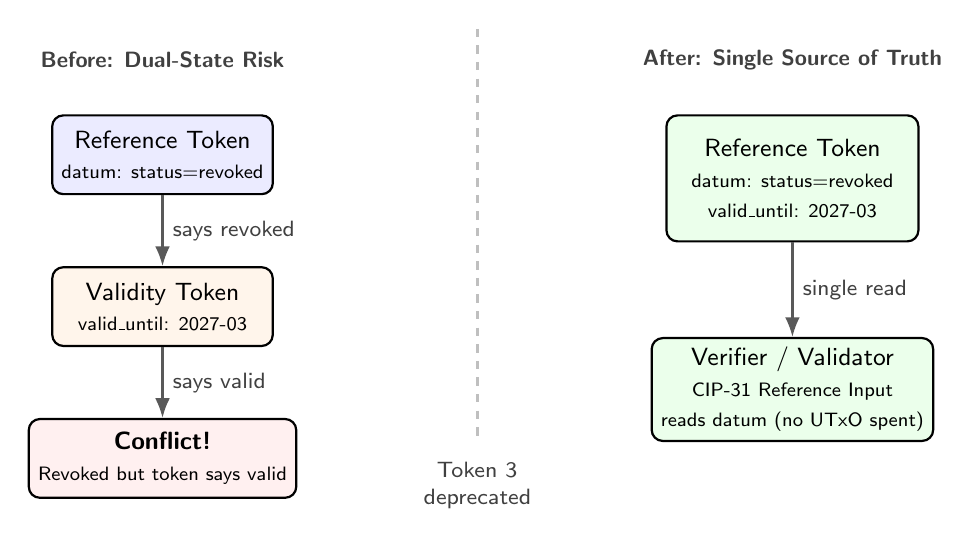
\begin{tikzpicture}[node distance=1.2cm and 1.8cm]
  % ── Before: Dual State ──
  \node[guidelabel] at (-4, 3.6) {\textbf{Before: Dual-State Risk}};

  \node[guidebox, fill=blue!8, minimum width=2.8cm] (refbefore)
    at (-4, 2.4) {Reference Token\\{\scriptsize\textsf{datum: status=revoked}}};

  \node[guidebox, fill=orange!8, minimum width=2.8cm, below=0.9cm of refbefore]
    (valtok) {Validity Token\\{\scriptsize\textsf{valid\_until: 2027-03}}};

  \node[guidebox, fill=red!6, minimum width=3cm, below=0.9cm of valtok]
    (conflict) {\textbf{Conflict!}\\{\scriptsize\textsf{Revoked but token says valid}}};

  \draw[guidearrow] (refbefore) -- node[guidelabel, right] {says revoked} (valtok);
  \draw[guidearrow] (valtok) -- node[guidelabel, right] {says valid} (conflict);

  % ── After: Single Source ──
  \node[guidelabel] at (4, 3.6) {\textbf{After: Single Source of Truth}};

  \node[guidebox, fill=green!8, minimum width=3.2cm, minimum height=1.6cm] (refafter)
    at (4, 2.1) {Reference Token\\{\scriptsize\textsf{datum: status=revoked}}\\
     {\scriptsize\textsf{valid\_until: 2027-03}}};

  \node[guidebox, fill=green!8, minimum width=3cm, below=1.2cm of refafter]
    (verifier) {Verifier / Validator\\{\scriptsize\textsf{CIP-31 Reference Input}}\\
     {\scriptsize\textsf{reads datum (no UTxO spent)}}};

  \draw[guidearrow] (refafter) -- node[guidelabel, right] {single read} (verifier);

  % ── Annotation ──
  \draw[dashed, thick, gray!50] (0, 4) -- (0, -1.2);
  \node[guidelabel, text width=2.5cm, align=center] at (0, -1.8)
    {Token~3\\deprecated};
\end{tikzpicture}
\caption{Validity token consolidation: before (left), the Reference Token and
  Validity Token can contradict each other.  After (right), all status and
  validity information resides in the Reference Token's datum, readable via
  CIP-31 Reference Input.}
\label{fig:validity-consolidation}
\end{figure}


% ----------------------------------------------------------------------------
\section{HSM Authority Keys}
\label{sec:hsm}

In the current implementation, authority wallet private keys are encrypted
with AES-256-GCM using a password-derived key (PBKDF2-HMAC-SHA256 with
100\,000 iterations) and stored as files on the server's filesystem.  While
this provides strong cryptographic protection against offline attacks, the
keys are still \emph{software-managed}: they are decrypted into process
memory during signing operations, and a sufficiently privileged attacker
with server access could potentially extract them.

Hardware Security Modules (HSMs) provide a fundamentally stronger security
model.  An HSM is a dedicated cryptographic processor that generates, stores,
and uses keys entirely within a tamper-resistant hardware enclave.  The
critical property is that private keys \emph{never leave the HSM}---not even
during signing.  When the application needs to sign a transaction, it sends
the transaction hash to the HSM, and the HSM returns the signature.  The
private key material is never exposed to the host operating system, the
application process, or any software layer.

For the credential verification system, HSM integration means that the
authority's signing key---the key that controls who can mint license NFTs,
revoke credentials, and deploy smart contracts---would be protected at the
hardware level.  Even if an attacker gained root access to the server, they
could not extract the authority key.  They could potentially \emph{use} the
HSM to sign transactions (if they gained access to the HSM's authentication
credentials), but they could not \emph{steal} the key for use elsewhere.

The v4.0 HSM integration plan targets PKCS\#11-compatible HSMs, which
include cloud-hosted options (AWS CloudHSM, Azure Dedicated HSM, Google
Cloud HSM) and on-premises devices (Thales Luna, Utimaco CryptoServer).
The \texttt{crypto.py} module will be extended with an HSM backend that
implements the same \texttt{encrypt\_key}/\texttt{decrypt\_key} interface,
allowing the rest of the codebase to use HSM-backed keys without
modification.


% ----------------------------------------------------------------------------
\section{KERI / Multi-Sig Upgrade}
\label{sec:keri-multisig}

The current system architecture concentrates all authority operations behind
a single signing key.  Whoever controls that key can mint credentials,
revoke licenses, deploy smart contracts, and collect dues payments.  This
single-key design was identified as finding AS-6 in the v3.0 security audit:
a single point of failure that, if compromised, could undermine the entire
credential system for that authority.

The v4.0 roadmap addresses this with two alternative approaches to
distributed governance, either of which eliminates the single-key risk.

\textbf{Option A: KERI (Key Event Receipt Infrastructure).}
KERI, standardized through the Veridian project, provides a decentralized
key-management framework where key authority is established through a
cryptographically linked sequence of key events (inception, rotation,
delegation) rather than through a single static key.  In a KERI-based
authority model, the credential-issuing authority would be identified by its
KERI Autonomic Identifier (AID), and key rotation events would allow the
authority to update its signing keys without invalidating previously issued
credentials.  This provides resilience against key compromise: if a key is
suspected of being compromised, the authority can rotate to a new key pair,
and all future operations use the new key while past operations remain
verifiable through the key-event log.

\textbf{Option B: Cardano ScriptNofK Multi-Signature.}
Cardano's native scripting system supports $N$-of-$K$ multi-signature
policies through the \texttt{ScriptNofK} constructor.  A 3-of-5
configuration, for example, would require any three out of five designated
board members to co-sign every authority operation.  This distributes trust
across multiple individuals and eliminates the single-key bottleneck.

In practical terms, a 3-of-5 multi-sig policy means that minting a new
license NFT requires three board members to independently sign the
transaction.  Revoking a credential requires three signatures.  Deploying a
new smart contract requires three signatures.  No single individual---and no
single compromised key---can perform any authority action alone.

The choice between KERI and multi-sig depends on the deploying
organization's requirements.  KERI provides more sophisticated key
management (rotation, delegation, recovery) but requires infrastructure for
maintaining the key-event log.  Multi-sig is simpler to implement using
Cardano's native scripting but does not support key rotation without
creating a new policy (and thus new policy ID).  Both approaches achieve the
primary goal: eliminating the single-key centralization risk identified in
AS-6.


% ----------------------------------------------------------------------------
\section{Security Audit Results}
\label{sec:audit}

The credential verification system underwent three rounds of architectural
security audit in February 2026, progressing from initial finding
identification through remediation verification to final clearance.

\subsection{v3.0 Audit: Initial Findings}

The first audit round examined the v3.0 architecture and identified five
findings across three severity levels:

\begin{itemize}[nosep]
  \item \textbf{2 Critical findings:}
    \begin{enumerate}[nosep]
      \item \emph{Single-key authority risk (AS-6):} All authority operations
        depend on a single signing key.  Compromise of this key would allow
        an attacker to mint fraudulent credentials, revoke legitimate ones,
        or deploy malicious smart contracts.
      \item \emph{Dual-state validity inconsistency:} The CIP-68 Reference
        Token datum and the standalone Validity Token can hold contradictory
        state, creating a class of verification errors.
    \end{enumerate}
  \item \textbf{1 High finding:}
    \begin{enumerate}[nosep]
      \item \emph{Software-managed authority keys:} Private keys decrypted
        into process memory during signing operations are vulnerable to
        memory-extraction attacks by privileged processes.
    \end{enumerate}
  \item \textbf{2 Medium findings:}
    \begin{enumerate}[nosep]
      \item \emph{Per-transaction script attachment overhead:} Attaching full
        validator bytecode to every transaction increases fees and exposes the
        compiled script to analysis.
      \item \emph{PlutusTx compilation inefficiency:} The Haskell-based
        compilation pipeline produces unnecessarily large UPLC output.
    \end{enumerate}
\end{itemize}

\subsection{v3.1 Audit: Remediation Verification}

The second audit round verified that all five findings from the v3.0 audit
had been addressed with concrete remediation plans:

\begin{itemize}[nosep]
  \item AS-6 (single-key risk): addressed by the KERI/multi-sig upgrade
    (Section~\ref{sec:keri-multisig})
  \item Dual-state inconsistency: addressed by validity-token consolidation
    (Section~\ref{sec:validity-consolidation})
  \item Software-managed keys: addressed by HSM integration
    (Section~\ref{sec:hsm})
  \item Script attachment overhead: addressed by CIP-33 reference scripts
    (Section~\ref{sec:cip33})
  \item PlutusTx inefficiency: addressed by Aiken migration
    (Section~\ref{sec:aiken})
\end{itemize}

\subsection{Final Audit: Testnet Clearance}

The third and final audit round confirmed that the remediation plans were
architecturally sound and that the v3.1 implementation (with the v4.0
roadmap items scheduled for implementation) was cleared for testnet
deployment.  All three audit reports are published in the project
repository.

The audit progression demonstrates a disciplined approach to security
engineering: identify weaknesses, design mitigations, verify the mitigations
address the root causes, and document everything.  The v4.0 roadmap items
described in this chapter are the direct result of this audit process.


% ============================================================================
%  PART C — GLOSSARY
% ============================================================================

\vspace{1em}
\noindent\rule{\textwidth}{0.8pt}
\begin{center}
  {\Large\sffamily\bfseries Part C --- Glossary}
\end{center}
\noindent\rule{\textwidth}{0.4pt}
\vspace{0.5em}

\section{Glossary of Terms}
\label{sec:glossary}

The following glossary defines every significant technical term used
throughout this study guide, organized alphabetically.

\begin{description}[style=nextline, leftmargin=2.5cm, labelwidth=2.3cm]

\item[ADA]
  The native cryptocurrency of the Cardano blockchain.  One ADA equals
  1\,000\,000 lovelace.  ADA is used to pay transaction fees, satisfy
  minimum UTxO requirements, and transfer value between addresses.

\item[AES-256-GCM]
  Advanced Encryption Standard with 256-bit keys in Galois/Counter Mode.
  An authenticated encryption algorithm that provides both confidentiality
  and integrity.  Used by \texttt{cardano-license} to encrypt wallet private
  keys at rest, with key derivation via PBKDF2-HMAC-SHA256 (100\,000
  iterations).

\item[Aiken]
  A modern smart-contract language for Cardano with Rust-like syntax.
  Compiles directly to UPLC bytecode, producing significantly smaller output
  than the PlutusTx/Haskell pipeline.  Planned for v4.0 to replace
  Haskell-compiled validators.

\item[Asset Name]
  The human-readable identifier for a native token within a minting policy.
  Combined with the Policy~ID to form a globally unique token identifier.
  In the credential system, asset names encode the license holder's
  identifier (e.g., \texttt{PE-2026-00142}).

\item[Base Address]
  A Cardano address that combines both a payment credential (derived from
  the payment key) and a staking credential (derived from the stake key).
  This is the standard address format used by the credential system, enabling
  both spending and staking from the same address.

\item[BIP-39]
  Bitcoin Improvement Proposal~39: a standard for generating deterministic
  wallet seeds from mnemonic word sequences.  The credential system uses
  24-word BIP-39 mnemonics as the root entropy for all wallet derivation.

\item[BIP-44]
  Bitcoin Improvement Proposal~44: a standard for hierarchical deterministic
  (HD) wallet derivation paths.  Superseded by CIP-1852 for Cardano-specific
  derivation, but the underlying multi-level derivation concept remains the
  same.

\item[Blake2b]
  A cryptographic hash function used extensively in Cardano for address
  derivation, script hashing, and transaction identification.  Cardano uses
  Blake2b-224 (28~bytes) for key hashes and Blake2b-256 (32~bytes) for
  transaction hashes.

\item[Blockfrost]
  A hosted API service that provides access to the Cardano blockchain without
  running a full node.  Supports UTxO queries, transaction submission,
  metadata retrieval, and block monitoring.  Used by \texttt{cardano-license}
  as the default chain backend.

\item[CIP-25]
  Cardano Improvement Proposal~25: the metadata standard for NFTs on
  Cardano.  Defines how token metadata (name, image, description, attributes)
  is attached to minting transactions under metadata label~721.  Used for
  license NFT metadata in the credential system.

\item[CIP-30]
  Cardano Improvement Proposal~30: the wallet connector standard that defines
  a JavaScript API for web applications to interact with Cardano wallets
  (e.g., Nami, Eternl).  Enables browser-based credential verification
  interfaces.

\item[CIP-31]
  Cardano Improvement Proposal~31: Reference Inputs.  Allows transactions to
  read the datum of a UTxO without consuming it.  Critical for the
  validity-token consolidation design, where verifiers read the Reference
  Token's datum without spending the authority's UTxO.

\item[CIP-32]
  Cardano Improvement Proposal~32: Inline Datums.  Allows datums to be
  stored directly in transaction outputs rather than as hashes.  Eliminates
  the need for datum witnesses in spending transactions and enables CIP-31
  reference-input reads.

\item[CIP-33]
  Cardano Improvement Proposal~33: Reference Scripts.  Allows Plutus
  scripts to be deployed once on-chain and referenced by subsequent
  transactions, eliminating the need to attach full script bytecode to every
  transaction.  See Section~\ref{sec:cip33}.

\item[CIP-68]
  Cardano Improvement Proposal~68: an NFT standard that splits each token
  into a Reference Token (label~100, held by the issuer, mutable datum) and a
  User Token (label~222, held by the recipient, immutable).  The credential
  system uses CIP-68 for authority-controlled revocation: the authority
  updates the Reference Token's datum without touching the licensee's wallet.

\item[CIP-1852]
  Cardano Improvement Proposal~1852: the HD wallet derivation standard for
  Cardano.  Defines derivation paths using purpose~1852, coin type~1815
  (Cardano), and separates payment keys (role~0) from stake keys (role~2).
  Path format: \texttt{m/1852'/1815'/0'/\{role\}/\{index\}}.

\item[Crypto-shredding]
  A data-destruction technique where encrypted data is rendered permanently
  inaccessible by destroying the encryption key rather than the ciphertext.
  Used in the credential system's GDPR compliance design: personal data
  stored off-chain under AES-256-GCM can be ``erased'' by deleting the
  encryption key, while the on-chain attestation hash remains.

\item[Datum]
  Data attached to a UTxO on the Cardano blockchain.  In the eUTxO model,
  datums serve as the state of smart contracts.  The credential system uses
  datums to store license status, validity windows, signer deposits, and
  dues-contract parameters.  See also: Inline Datum, CIP-32.

\item[DID]
  Decentralized Identifier: a W3C standard for self-sovereign digital
  identities.  DIDs are URI-formatted identifiers that can be resolved to
  DID Documents containing public keys, service endpoints, and
  authentication methods.  Related to KERI's approach to decentralized
  identity.

\item[eIDAS]
  Electronic Identification, Authentication and Trust Services: the European
  Union regulation establishing a legal framework for electronic signatures,
  seals, timestamps, and identification.  eIDAS~2.0 introduces the European
  Digital Identity Wallet.  The credential system's on-chain signatures align
  with eIDAS requirements for advanced electronic signatures.

\item[ESIGN Act]
  The Electronic Signatures in Global and National Commerce Act (2000): a
  United States federal law that grants electronic signatures the same legal
  standing as handwritten signatures.  Together with UETA, establishes the
  legal foundation for blockchain-based professional credential signatures.

\item[eUTxO]
  Extended Unspent Transaction Output: Cardano's transaction model that
  extends Bitcoin's UTxO model with datums (state), redeemers (actions), and
  script contexts (validators).  The eUTxO model provides deterministic
  transaction validation and enables the credential system's per-signer
  deposit design for concurrent signing.

\item[Epoch]
  A time period in the Cardano blockchain, lasting approximately 5~days
  (432\,000 slots on mainnet).  Epochs are relevant to the credential system
  for stake-reward distribution and protocol-parameter updates that affect
  transaction fees and minUTxO values.

\item[exUnits]
  Execution units: a two-dimensional measure of Plutus script resource
  consumption on Cardano, comprising CPU steps and memory units.  Each
  transaction has maximum exUnit budgets.  Smaller exUnit consumption (e.g.,
  from Aiken-compiled scripts) translates to lower fees and higher
  throughput.

\item[GDPR]
  General Data Protection Regulation: the European Union's data-privacy law
  that includes the ``right to erasure'' (Article~17).  The credential
  system's off-chain personal-data storage with crypto-shredding is designed
  to satisfy GDPR requirements while maintaining on-chain attestation
  immutability.

\item[Halo2]
  A zero-knowledge proof system based on polynomial commitments, developed by
  the Electric Coin Company.  Relevant to future privacy-preserving
  credential verification where a holder can prove possession of a valid
  credential without revealing the credential's details.

\item[HD Wallet]
  Hierarchical Deterministic wallet: a wallet architecture where a single
  seed (mnemonic) can derive an unlimited tree of key pairs using
  deterministic derivation paths (BIP-32/BIP-44/CIP-1852).  The credential
  system uses HD wallets for all participant roles.

\item[HSM]
  Hardware Security Module: a dedicated cryptographic processor that
  generates, stores, and uses keys within a tamper-resistant hardware
  enclave.  Private keys never leave the HSM.  Planned for v4.0 to protect
  authority signing keys.  See Section~\ref{sec:hsm}.

\item[Inline Datum]
  A datum stored directly in a transaction output (enabled by CIP-32),
  rather than as a hash that must be provided as a witness during spending.
  Inline datums enable CIP-31 reference-input reads, which are essential for
  the validity-token consolidation design.

\item[KERI]
  Key Event Receipt Infrastructure: a decentralized key-management protocol
  standardized through the Veridian project.  KERI establishes key authority
  through a cryptographically linked sequence of key events (inception,
  rotation, delegation, interaction).  Planned for v4.0 as one option for
  distributed authority governance.  See Section~\ref{sec:keri-multisig}.

\item[Lovelace]
  The smallest unit of ADA.  One ADA equals 1\,000\,000 lovelace.  Named
  after Ada Lovelace.  All on-chain amounts in the credential system are
  denominated in lovelace.

\item[minUTxO]
  The protocol-enforced minimum amount of ADA that must accompany any UTxO.
  The value depends on the UTxO's size (datum size, number of native tokens).
  The credential system uses a conservative default of 2~ADA
  (2\,000\,000~lovelace) for token-bearing outputs.

\item[Minting Policy]
  A script that governs the creation and destruction of native tokens on
  Cardano.  The credential system uses authority-key-restricted
  \texttt{ScriptPubkey} policies (Native Script) that permit only the
  authority's signing key to mint or burn tokens under that policy.

\item[Native Script]
  A simple scripting language on Cardano (predating Plutus) that supports
  key-signature requirements, time locks, and Boolean combinations
  (all-of, any-of, $N$-of-$K$).  The credential system uses Native Scripts
  for minting policies.  Multi-sig governance would use
  \texttt{ScriptNofK}.

\item[NFT]
  Non-Fungible Token: a unique token with quantity~1.  On Cardano, NFTs are
  native multi-asset tokens with an enforced quantity of one.  License NFTs
  in the credential system are NFTs carrying CIP-25 metadata that attests to
  a professional's credential.

\item[Ouroboros]
  The family of proof-of-stake consensus protocols used by Cardano.
  Ouroboros Praos (the current production variant) provides probabilistic
  finality and is formally verified for security properties.  Relevant to
  the credential system because consensus determines when minted credentials
  become final.

\item[PKH]
  Public Key Hash: the Blake2b-224 hash of a verification (public) key.  Used
  as the payment credential in Cardano addresses and as the identity
  parameter in minting policies.  The credential system's authority-restricted
  policies require the authority's PKH to authorize minting.

\item[Plutus]
  The smart-contract platform on Cardano, based on the eUTxO model.  Plutus
  scripts (validators) run on-chain to enforce spending conditions.  The
  credential system uses Plutus~V2 for the signature-collection validator and
  the dues-enforcement contract.

\item[Policy ID]
  The hash of a minting policy script.  Serves as the unique, immutable
  identifier for all tokens minted under that policy.  In the credential
  system, the Policy~ID cryptographically binds every license NFT,
  signature token, and validity token to the authority that created the
  minting policy.

\item[PyCardano]
  A Python library for building Cardano transactions, managing wallets, and
  interacting with the blockchain.  Provides HD~wallet generation, Plutus~V2
  script support, and CIP-1852 derivation.  The primary Cardano SDK used by
  \texttt{cardano-license}.

\item[Redeemer]
  Data provided by a transaction to a Plutus validator, specifying the
  intended action.  In the credential system, redeemers include
  \texttt{CollectRedeemer} (deposit a signature), \texttt{FinalizeRedeemer}
  (sweep all deposits), \texttt{ReclaimRedeemer} (reclaim a deposit),
  \texttt{PayDuesRedeemer} (pay dues), and \texttt{RevokeValidityRedeemer}
  (revoke for non-payment).

\item[Reference Input]
  A transaction input (enabled by CIP-31) that reads a UTxO's datum without
  consuming the UTxO.  Essential for the validity-consolidation design,
  where verifiers read the Reference Token's datum without spending the
  authority's UTxO.  See CIP-31.

\item[Reference Script]
  A Plutus script stored on-chain in a UTxO (enabled by CIP-33) that can be
  referenced by subsequent transactions instead of being attached inline.
  Reduces transaction size and fees.  See Section~\ref{sec:cip33}.

\item[Reference Token]
  In the CIP-68 standard, the token with label~100 that is held by the
  issuing authority and carries a mutable inline datum.  The credential
  system uses Reference Tokens for authority-controlled status management:
  the authority updates the datum to revoke or suspend a credential without
  interacting with the licensee's wallet.

\item[Script Context]
  The information available to a Plutus validator during execution: the
  transaction being validated (inputs, outputs, minting, fees, validity
  range, signatories), the script's own purpose (spending, minting,
  certifying), and the datum and redeemer.  Validators use the Script Context
  to enforce spending conditions.

\item[Slot]
  The fundamental time unit on the Cardano blockchain, lasting 1~second on
  mainnet.  Slots are used in validity ranges (\texttt{InvalidBefore},
  \texttt{InvalidHereAfter}) and in time-locked minting policies.  The
  credential system converts between POSIX timestamps and slot numbers for
  validity-window enforcement.

\item[Stake Key]
  The key pair used for staking operations in a Cardano HD~wallet.  Derived
  from path \texttt{m/1852'/1815'/0'/2/0}.  Combined with the payment key to
  form a base address.  The credential system derives stake keys for all
  wallet types but uses them primarily for address construction.

\item[UETA]
  Uniform Electronic Transactions Act (1999): a U.S. model law (adopted by
  47 states) that establishes the legal validity of electronic records and
  signatures.  Together with the ESIGN Act, provides the legal foundation
  for blockchain-based credential signatures.

\item[UPLC]
  Untyped Plutus Lambda Calculus: the low-level execution language for
  Plutus smart contracts on Cardano.  Both PlutusTx (Haskell) and Aiken
  compile down to UPLC bytecode.  Smaller UPLC output means lower exUnit
  consumption and lower fees.

\item[User Token]
  In the CIP-68 standard, the token with label~222 that is held by the
  recipient (licensee).  The User Token is immutable and serves as the
  holder's proof of credential issuance.  Its counterpart, the Reference
  Token (label~100), is held by the authority and carries the mutable status
  datum.

\item[UTxO]
  Unspent Transaction Output: the fundamental unit of value on the Cardano
  blockchain.  Each UTxO contains an address, a value (ADA and/or native
  tokens), and optionally a datum.  Spending a UTxO consumes it entirely and
  creates new UTxOs.  The credential system's per-signer deposit design
  creates independent UTxOs to avoid concurrency conflicts.

\item[Validator]
  A Plutus script that governs the conditions under which a UTxO can be
  spent.  The credential system uses two validators: the
  signature-collection validator (manages multi-signer deposits and
  finalization) and the dues-enforcement validator (links credential
  validity to payment obligations).

\item[Veridian]
  The open-source project (formerly under the Trust over IP Foundation) that
  develops the KERI protocol and ACDC (Authentic Chained Data Container)
  standards for decentralized identity and verifiable credentials.  The v4.0
  roadmap considers Veridian/KERI as one option for distributed authority
  governance.

\end{description}


% ============================================================================
\end{document}
